
%% $Id$

\documentclass[12pt]{report}
\usepackage{graphicx,a4,../iman,../extra,../proof,../rail,../pdfsetup}

\title{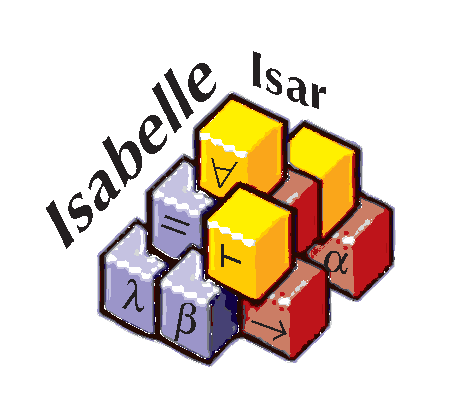
\includegraphics[scale=0.5]{isabelle_isar} \\[4ex] The Isabelle/Isar Reference Manual}

\author{\emph{Markus Wenzel} \\ TU M\"unchen}

\setcounter{secnumdepth}{2} \setcounter{tocdepth}{2}

\pagestyle{headings}
\sloppy
\binperiod     %%%treat . like a binary operator

\railalias{lbrace}{\ttlbrace}
\railalias{rbrace}{\ttrbrace}
\railterm{lbrace,rbrace}

\railterm{ident,longident,symident,var,textvar,typefree,typevar,nat,string,verbatim}


\begin{document}

\underscoreoff

\maketitle 

\begin{abstract}
  FIXME
\end{abstract}

\pagenumbering{roman} \tableofcontents \clearfirst

%FIXME
\nocite{Rudnicki:1992:MizarOverview}
\nocite{Harrison:1996:MizarHOL}
\nocite{Rudnicki:1992:MizarOverview}
\nocite{Trybulec:1993:MizarFeatures}
\nocite{Syme:1997:DECLARE}
\nocite{Syme:1998:thesis}
\nocite{Syme:1999:TPHOL}
\nocite{Wenzel:1999:TPHOL}


\chapter{Introduction}

\section{Quick start}

Isar is already part of Isabelle (as of version Isabelle99, or later).  The
\texttt{isabelle} binary provides option \texttt{-I} to run the Isar
interaction loop at startup, rather than the plain ML top-level.  Thus the
quickest way to do anything with Isabelle/Isar is as follows:
\begin{ttbox}
isabelle -I HOL\medskip
\out{> Welcome to Isabelle/HOL (Isabelle99)}\medskip
theory Foo = Main:
constdefs foo :: nat  "foo == 1";
lemma "0 < foo" by (simp add: foo_def);
end
\end{ttbox}
Note that any Isabelle/Isar command may be retracted by \texttt{undo}.

Plain TTY-based interaction like this used to be quite feasible with
traditional tactic based theorem proving, but developing Isar documents
demands some better user-interface support.  \emph{Proof~General}\index{Proof
  General} of LFCS Edinburgh \cite{proofgeneral} offers a generic Emacs-based
environment for interactive theorem provers that does all the cut-and-paste
and forward-backward walk through the document in a very neat way.  Note that
in Isabelle/Isar, the current position within a partial proof document is more
informative than the actual proof state.  Thus Proof~General provides the
canonical working environment for Isabelle/Isar, both for getting acquainted
(e.g.\ by replaying existing Isar documents) and serious production work.

\medskip

The easiest way to use Proof~General is to make it the default Isabelle user
interface.  Just say something like this in your Isabelle settings file (cf.\ 
\cite{isabelle-sys}):
\begin{ttbox}
ISABELLE_INTERFACE=\$ISABELLE_HOME/contrib/ProofGeneral/isar/interface
PROOFGENERAL_OPTIONS=""
\end{ttbox}
You may have to change \texttt{\$ISABELLE_HOME/contrib/ProofGeneral} to the
actual installation directory of Proof~General.  From now on, the capital
\texttt{Isabelle} executable refers to the \texttt{ProofGeneral/isar}
interface.  Its usage is as follows:
\begin{ttbox}
Usage: interface [OPTIONS] [FILES ...]

  Options are:
    -l NAME      logic image name (default $ISABELLE_LOGIC=HOL)
    -p NAME      Emacs program name (default xemacs)
    -u BOOL      use .emacs file (default true)
    -w BOOL      use window system (default true)

  Starts Proof General for Isabelle/Isar with proof documents FILES
  (default Scratch.thy).

  PROOFGENERAL_OPTIONS=
\end{ttbox}
Apart from the command line, the defaults for these options may be overridden
via the \texttt{PROOFGENERAL_OPTIONS} setting as well.  For example, plain GNU
Emacs may be configured as follows:
\begin{ttbox}
PROOFGENERAL_OPTIONS="-p emacs"
\end{ttbox}

With the proper Isabelle interface setup, Isar documents may now be edited by
visiting appropriate theory files, e.g.\ 
\begin{ttbox}
Isabelle \({\langle}isabellehome{\rangle}\)/src/HOL/Isar_examples/BasicLogic.thy
\end{ttbox}
Users of XEmacs may note the tool bar for navigating forward and backward
through the text.  Consult the Proof~General documentation \cite{proofgeneral}
for further basic commands, such as \texttt{c-c return} or \texttt{c-c u}.

\medskip

Occasionally, a user's \texttt{.emacs} contains material that is incompatible
with the version of (X)Emacs that Proof~General prefers.  Then proper startup
may be still achieved by using the \texttt{-u false} option.\footnote{Also
  note that the Emacs lisp files
  \texttt{\$ISABELLE_HOME/etc/proofgeneral-settings.el} and
  \texttt{\$ISABELLE_HOME_USER/etc/proofgeneral-settings.el} are automatically
  loaded by Proof~General if invoked via the interface wrapper script.}


\section{How to write Isar proofs anyway?}

This is one of the key questions, of course.  Isar offers a rather different
approach to formal proof documents than plain old tactic scripts.  Experienced
users of existing interactive theorem proving systems may have to learn
thinking different in order to make effective use of Isabelle/Isar.  On the
other hand, Isabelle/Isar comes much closer to existing mathematical practice
of formal proof, so users with less experience in old-style tactical proving,
but a good understanding of mathematical proof might cope with Isar even
better.

Unfortunately, there is no tutorial on Isabelle/Isar available yet.  This
document really is a \emph{reference manual}.  Nevertheless, we will give some
discussions of the general principles underlying Isar in
chapter~\ref{ch:basics}, and provide some clues of how these may be put into
practice.  Some more background information on Isar is given in
\cite{Wenzel:1999:TPHOL}.  Furthermore, there are several examples distributed
with Isabelle (see directory \texttt{HOL/Isar_examples}).


%%% Local Variables: 
%%% mode: latex
%%% TeX-master: "isar-ref"
%%% End: 

\chapter{The Basics}

\section{Introduction}

This book is a tutorial on how to use the theorem prover Isabelle/HOL as a
specification and verification system. Isabelle is a generic system for
implementing logical formalisms, and Isabelle/HOL is the specialization
of Isabelle for HOL, which abbreviates Higher-Order Logic. We introduce
HOL step by step following the equation
\[ \mbox{HOL} = \mbox{Functional Programming} + \mbox{Logic}. \]
We do not assume that you are familiar with mathematical logic. 
However, we do assume that
you are used to logical and set theoretic notation, as covered
in a good discrete mathematics course~\cite{Rosen-DMA}, and
that you are familiar with the basic concepts of functional
programming~\cite{Bird-Haskell,Hudak-Haskell,paulson-ml2,Thompson-Haskell}.
Although this tutorial initially concentrates on functional programming, do
not be misled: HOL can express most mathematical concepts, and functional
programming is just one particularly simple and ubiquitous instance.

Isabelle~\cite{paulson-isa-book} is implemented in ML~\cite{SML}.  This has
influenced some of Isabelle/HOL's concrete syntax but is otherwise irrelevant
for us: this tutorial is based on
Isabelle/Isar~\cite{isabelle-isar-ref}, an extension of Isabelle which hides
the implementation language almost completely.  Thus the full name of the
system should be Isabelle/Isar/HOL, but that is a bit of a mouthful.

There are other implementations of HOL, in particular the one by Mike Gordon
\index{Gordon, Mike}%
\emph{et al.}, which is usually referred to as ``the HOL system''
\cite{mgordon-hol}. For us, HOL refers to the logical system, and sometimes
its incarnation Isabelle/HOL\@.

A tutorial is by definition incomplete.  Currently the tutorial only
introduces the rudiments of Isar's proof language. To fully exploit the power
of Isar, in particular the ability to write readable and structured proofs,
you need to consult the Isabelle/Isar Reference
Manual~\cite{isabelle-isar-ref} and Wenzel's PhD thesis~\cite{Wenzel-PhD}
which discusses many proof patterns. If you want to use Isabelle's ML level
directly (for example for writing your own proof procedures) see the Isabelle
Reference Manual~\cite{isabelle-ref}; for details relating to HOL see the
Isabelle/HOL manual~\cite{isabelle-HOL}. All manuals have a comprehensive
index.

\section{Theories}
\label{sec:Basic:Theories}

\index{theories|(}%
Working with Isabelle means creating theories. Roughly speaking, a
\textbf{theory} is a named collection of types, functions, and theorems,
much like a module in a programming language or a specification in a
specification language. In fact, theories in HOL can be either. The general
format of a theory \texttt{T} is
\begin{ttbox}
theory T
imports B\(@1\) \(\ldots\) B\(@n\)
begin
{\rmfamily\textit{declarations, definitions, and proofs}}
end
\end{ttbox}\cmmdx{theory}\cmmdx{imports}
where \texttt{B}$@1$ \dots\ \texttt{B}$@n$ are the names of existing
theories that \texttt{T} is based on and \textit{declarations,
    definitions, and proofs} represents the newly introduced concepts
(types, functions etc.) and proofs about them. The \texttt{B}$@i$ are the
direct \textbf{parent theories}\indexbold{parent theories} of~\texttt{T}\@.
Everything defined in the parent theories (and their parents, recursively) is
automatically visible. To avoid name clashes, identifiers can be
\textbf{qualified}\indexbold{identifiers!qualified}
by theory names as in \texttt{T.f} and~\texttt{B.f}. 
Each theory \texttt{T} must
reside in a \textbf{theory file}\index{theory files} named \texttt{T.thy}.

This tutorial is concerned with introducing you to the different linguistic
constructs that can fill the \textit{declarations, definitions, and
    proofs} above.  A complete grammar of the basic
constructs is found in the Isabelle/Isar Reference
Manual~\cite{isabelle-isar-ref}.

HOL's theory collection is available online at
\begin{center}\small
    \url{http://isabelle.in.tum.de/library/HOL/}
\end{center}
and is recommended browsing. Note that most of the theories 
are based on classical Isabelle without the Isar extension. This means that
they look slightly different than the theories in this tutorial, and that all
proofs are in separate ML files.

\begin{warn}
  HOL contains a theory \thydx{Main}, the union of all the basic
  predefined theories like arithmetic, lists, sets, etc.  
  Unless you know what you are doing, always include \isa{Main}
  as a direct or indirect parent of all your theories.
\end{warn}
There is also a growing Library~\cite{HOL-Library}\index{Library}
of useful theories that are not part of \isa{Main} but can be included
among the parents of a theory and will then be loaded automatically.%
\index{theories|)}


\section{Types, Terms and Formulae}
\label{sec:TypesTermsForms}

Embedded in a theory are the types, terms and formulae of HOL\@. HOL is a typed
logic whose type system resembles that of functional programming languages
like ML or Haskell. Thus there are
\index{types|(}
\begin{description}
\item[base types,] 
in particular \tydx{bool}, the type of truth values,
and \tydx{nat}, the type of natural numbers.
\item[type constructors,]\index{type constructors}
 in particular \tydx{list}, the type of
lists, and \tydx{set}, the type of sets. Type constructors are written
postfix, e.g.\ \isa{(nat)list} is the type of lists whose elements are
natural numbers. Parentheses around single arguments can be dropped (as in
\isa{nat list}), multiple arguments are separated by commas (as in
\isa{(bool,nat)ty}).
\item[function types,]\index{function types}
denoted by \isasymFun\indexbold{$IsaFun@\isasymFun}.
  In HOL \isasymFun\ represents \emph{total} functions only. As is customary,
  \isa{$\tau@1$ \isasymFun~$\tau@2$ \isasymFun~$\tau@3$} means
  \isa{$\tau@1$ \isasymFun~($\tau@2$ \isasymFun~$\tau@3$)}. Isabelle also
  supports the notation \isa{[$\tau@1,\dots,\tau@n$] \isasymFun~$\tau$}
  which abbreviates \isa{$\tau@1$ \isasymFun~$\cdots$ \isasymFun~$\tau@n$
    \isasymFun~$\tau$}.
\item[type variables,]\index{type variables}\index{variables!type}
  denoted by \ttindexboldpos{'a}{$Isatype}, \isa{'b} etc., just like in ML\@. They give rise
  to polymorphic types like \isa{'a \isasymFun~'a}, the type of the identity
  function.
\end{description}
\begin{warn}
  Types are extremely important because they prevent us from writing
  nonsense.  Isabelle insists that all terms and formulae must be well-typed
  and will print an error message if a type mismatch is encountered. To
  reduce the amount of explicit type information that needs to be provided by
  the user, Isabelle infers the type of all variables automatically (this is
  called \bfindex{type inference}) and keeps quiet about it. Occasionally
  this may lead to misunderstandings between you and the system. If anything
  strange happens, we recommend that you set the flag\index{flags}
  \isa{show_types}\index{*show_types (flag)}.  
  Isabelle will then display type information
  that is usually suppressed.  Simply type
\begin{ttbox}
ML "set show_types"
\end{ttbox}

\noindent
This can be reversed by \texttt{ML "reset show_types"}. Various other flags,
which we introduce as we go along, can be set and reset in the same manner.%
\index{flags!setting and resetting}
\end{warn}%
\index{types|)}


\index{terms|(}
\textbf{Terms} are formed as in functional programming by
applying functions to arguments. If \isa{f} is a function of type
\isa{$\tau@1$ \isasymFun~$\tau@2$} and \isa{t} is a term of type
$\tau@1$ then \isa{f~t} is a term of type $\tau@2$. HOL also supports
infix functions like \isa{+} and some basic constructs from functional
programming, such as conditional expressions:
\begin{description}
\item[\isa{if $b$ then $t@1$ else $t@2$}]\index{*if expressions}
Here $b$ is of type \isa{bool} and $t@1$ and $t@2$ are of the same type.
\item[\isa{let $x$ = $t$ in $u$}]\index{*let expressions}
is equivalent to $u$ where all free occurrences of $x$ have been replaced by
$t$. For example,
\isa{let x = 0 in x+x} is equivalent to \isa{0+0}. Multiple bindings are separated
by semicolons: \isa{let $x@1$ = $t@1$;\dots; $x@n$ = $t@n$ in $u$}.
\item[\isa{case $e$ of $c@1$ \isasymFun~$e@1$ |~\dots~| $c@n$ \isasymFun~$e@n$}]
\index{*case expressions}
evaluates to $e@i$ if $e$ is of the form $c@i$.
\end{description}

Terms may also contain
\isasymlambda-abstractions.\index{lambda@$\lambda$ expressions}
For example,
\isa{\isasymlambda{}x.~x+1} is the function that takes an argument \isa{x} and
returns \isa{x+1}. Instead of
\isa{\isasymlambda{}x.\isasymlambda{}y.\isasymlambda{}z.~$t$} we can write
\isa{\isasymlambda{}x~y~z.~$t$}.%
\index{terms|)}

\index{formulae|(}%
\textbf{Formulae} are terms of type \tydx{bool}.
There are the basic constants \cdx{True} and \cdx{False} and
the usual logical connectives (in decreasing order of priority):
\indexboldpos{\protect\isasymnot}{$HOL0not}, \indexboldpos{\protect\isasymand}{$HOL0and},
\indexboldpos{\protect\isasymor}{$HOL0or}, and \indexboldpos{\protect\isasymimp}{$HOL0imp},
all of which (except the unary \isasymnot) associate to the right. In
particular \isa{A \isasymimp~B \isasymimp~C} means \isa{A \isasymimp~(B
  \isasymimp~C)} and is thus logically equivalent to \isa{A \isasymand~B
  \isasymimp~C} (which is \isa{(A \isasymand~B) \isasymimp~C}).

Equality\index{equality} is available in the form of the infix function
\isa{=} of type \isa{'a \isasymFun~'a
  \isasymFun~bool}. Thus \isa{$t@1$ = $t@2$} is a formula provided $t@1$
and $t@2$ are terms of the same type. If $t@1$ and $t@2$ are of type
\isa{bool} then \isa{=} acts as \rmindex{if-and-only-if}.
The formula
\isa{$t@1$~\isasymnoteq~$t@2$} is merely an abbreviation for
\isa{\isasymnot($t@1$ = $t@2$)}.

Quantifiers\index{quantifiers} are written as
\isa{\isasymforall{}x.~$P$} and \isa{\isasymexists{}x.~$P$}. 
There is even
\isa{\isasymuniqex{}x.~$P$}, which
means that there exists exactly one \isa{x} that satisfies \isa{$P$}. 
Nested quantifications can be abbreviated:
\isa{\isasymforall{}x~y~z.~$P$} means
\isa{\isasymforall{}x.\isasymforall{}y.\isasymforall{}z.~$P$}.%
\index{formulae|)}

Despite type inference, it is sometimes necessary to attach explicit
\bfindex{type constraints} to a term.  The syntax is
\isa{$t$::$\tau$} as in \isa{x < (y::nat)}. Note that
\ttindexboldpos{::}{$Isatype} binds weakly and should therefore be enclosed
in parentheses.  For instance,
\isa{x < y::nat} is ill-typed because it is interpreted as
\isa{(x < y)::nat}.  Type constraints may be needed to disambiguate
expressions
involving overloaded functions such as~\isa{+}, 
\isa{*} and~\isa{<}.  Section~\ref{sec:overloading} 
discusses overloading, while Table~\ref{tab:overloading} presents the most
important overloaded function symbols.

In general, HOL's concrete \rmindex{syntax} tries to follow the conventions of
functional programming and mathematics.  Here are the main rules that you
should be familiar with to avoid certain syntactic traps:
\begin{itemize}
\item
Remember that \isa{f t u} means \isa{(f t) u} and not \isa{f(t u)}!
\item
Isabelle allows infix functions like \isa{+}. The prefix form of function
application binds more strongly than anything else and hence \isa{f~x + y}
means \isa{(f~x)~+~y} and not \isa{f(x+y)}.
\item Remember that in HOL if-and-only-if is expressed using equality.  But
  equality has a high priority, as befitting a relation, while if-and-only-if
  typically has the lowest priority.  Thus, \isa{\isasymnot~\isasymnot~P =
    P} means \isa{\isasymnot\isasymnot(P = P)} and not
  \isa{(\isasymnot\isasymnot P) = P}. When using \isa{=} to mean
  logical equivalence, enclose both operands in parentheses, as in \isa{(A
    \isasymand~B) = (B \isasymand~A)}.
\item
Constructs with an opening but without a closing delimiter bind very weakly
and should therefore be enclosed in parentheses if they appear in subterms, as
in \isa{(\isasymlambda{}x.~x) = f}.  This includes 
\isa{if},\index{*if expressions}
\isa{let},\index{*let expressions}
\isa{case},\index{*case expressions}
\isa{\isasymlambda}, and quantifiers.
\item
Never write \isa{\isasymlambda{}x.x} or \isa{\isasymforall{}x.x=x}
because \isa{x.x} is always taken as a single qualified identifier. Write
\isa{\isasymlambda{}x.~x} and \isa{\isasymforall{}x.~x=x} instead.
\item Identifiers\indexbold{identifiers} may contain the characters \isa{_} 
and~\isa{'}, except at the beginning.
\end{itemize}

For the sake of readability, we use the usual mathematical symbols throughout
the tutorial. Their \textsc{ascii}-equivalents are shown in table~\ref{tab:ascii} in
the appendix.

\begin{warn}
A particular
problem for novices can be the priority of operators. If you are unsure, use
additional parentheses. In those cases where Isabelle echoes your
input, you can see which parentheses are dropped --- they were superfluous. If
you are unsure how to interpret Isabelle's output because you don't know
where the (dropped) parentheses go, set the flag\index{flags}
\isa{show_brackets}\index{*show_brackets (flag)}:
\begin{ttbox}
ML "set show_brackets"; \(\dots\); ML "reset show_brackets";
\end{ttbox}
\end{warn}


\section{Variables}
\label{sec:variables}
\index{variables|(}

Isabelle distinguishes free and bound variables, as is customary. Bound
variables are automatically renamed to avoid clashes with free variables. In
addition, Isabelle has a third kind of variable, called a \textbf{schematic
  variable}\index{variables!schematic} or \textbf{unknown}\index{unknowns}, 
which must have a~\isa{?} as its first character.  
Logically, an unknown is a free variable. But it may be
instantiated by another term during the proof process. For example, the
mathematical theorem $x = x$ is represented in Isabelle as \isa{?x = ?x},
which means that Isabelle can instantiate it arbitrarily. This is in contrast
to ordinary variables, which remain fixed. The programming language Prolog
calls unknowns {\em logical\/} variables.

Most of the time you can and should ignore unknowns and work with ordinary
variables. Just don't be surprised that after you have finished the proof of
a theorem, Isabelle will turn your free variables into unknowns.  It
indicates that Isabelle will automatically instantiate those unknowns
suitably when the theorem is used in some other proof.
Note that for readability we often drop the \isa{?}s when displaying a theorem.
\begin{warn}
  For historical reasons, Isabelle accepts \isa{?} as an ASCII representation
  of the \(\exists\) symbol.  However, the \isa{?} character must then be followed
  by a space, as in \isa{?~x. f(x) = 0}.  Otherwise, \isa{?x} is
  interpreted as a schematic variable.  The preferred ASCII representation of
  the \(\exists\) symbol is \isa{EX}\@. 
\end{warn}%
\index{variables|)}

\section{Interaction and Interfaces}

Interaction with Isabelle can either occur at the shell level or through more
advanced interfaces. To keep the tutorial independent of the interface, we
have phrased the description of the interaction in a neutral language. For
example, the phrase ``to abandon a proof'' means to type \isacommand{oops} at the
shell level, which is explained the first time the phrase is used. Other
interfaces perform the same act by cursor movements and/or mouse clicks.
Although shell-based interaction is quite feasible for the kind of proof
scripts currently presented in this tutorial, the recommended interface for
Isabelle/Isar is the Emacs-based \bfindex{Proof
  General}~\cite{proofgeneral,Aspinall:TACAS:2000}.

Some interfaces (including the shell level) offer special fonts with
mathematical symbols. For those that do not, remember that \textsc{ascii}-equivalents
are shown in table~\ref{tab:ascii} in the appendix.

Finally, a word about semicolons.\indexbold{$Isar@\texttt{;}} 
Commands may but need not be terminated by semicolons.
At the shell level it is advisable to use semicolons to enforce that a command
is executed immediately; otherwise Isabelle may wait for the next keyword
before it knows that the command is complete.


\section{Getting Started}

Assuming you have installed Isabelle, you start it by typing \texttt{isabelle
  -I HOL} in a shell window.\footnote{Simply executing \texttt{isabelle -I}
  starts the default logic, which usually is already \texttt{HOL}.  This is
  controlled by the \texttt{ISABELLE_LOGIC} setting, see \emph{The Isabelle
    System Manual} for more details.} This presents you with Isabelle's most
basic \textsc{ascii} interface.  In addition you need to open an editor window to
create theory files.  While you are developing a theory, we recommend that you
type each command into the file first and then enter it into Isabelle by
copy-and-paste, thus ensuring that you have a complete record of your theory.
As mentioned above, Proof General offers a much superior interface.
If you have installed Proof General, you can start it by typing \texttt{Isabelle}.


\chapter{Syntax primitives}

The rather generic framework of Isabelle/Isar syntax emerges from three main
syntactic categories: \emph{commands} of the top-level Isar engine (covering
theory and proof elements), \emph{methods} for general goal refinements
(analogous to traditional ``tactics''), and \emph{attributes} for operations
on facts (within a certain context).  Here we give a reference of basic
syntactic entities underlying Isabelle/Isar syntax in a bottom-up manner.
Concrete theory and proof language elements will be introduced later on.

\medskip

In order to get started with writing well-formed Isabelle/Isar documents, the
most important aspect to be noted is the difference of \emph{inner} versus
\emph{outer} syntax.  Inner syntax is that of Isabelle types and terms of the
logic, while outer syntax is that of Isabelle/Isar theory sources (including
proofs).  As a general rule, inner syntax entities may occur only as
\emph{atomic entities} within outer syntax.  For example, the string
\texttt{"x + y"} and identifier \texttt{z} are legal term specifications
within a theory, while \texttt{x + y} is not.

\begin{warn}
  Old-style Isabelle theories used to fake parts of the inner syntax of types,
  with rather complicated rules when quotes may be omitted.  Despite the minor
  drawback of requiring quotes more often, the syntax of Isabelle/Isar is
  somewhat simpler and more robust in that respect.
\end{warn}

Printed theory documents usually omit quotes to gain readability (this is a
matter of {\LaTeX} macro setup, say via \verb,\isabellestyle,, see also
\cite{isabelle-sys}).  Experienced users of Isabelle/Isar may easily
reconstruct the lost technical information, while mere readers need not care
about quotes at all.

\medskip

Isabelle/Isar input may contain any number of input termination characters
``\texttt{;}'' (semicolon) to separate commands explicitly.  This is
particularly useful in interactive shell sessions to make clear where the
current command is intended to end.  Otherwise, the interpreter loop will
continue to issue a secondary prompt ``\verb,#,'' until an end-of-command is
clearly recognized from the input syntax, e.g.\ encounter of the next command
keyword.

Advanced interfaces such as Proof~General \cite{proofgeneral} do not require
explicit semicolons, the amount of input text is determined automatically by
inspecting the present content of the Emacs text buffer.  In the printed
presentation of Isabelle/Isar documents semicolons are omitted altogether for
readability.

\begin{warn}
  Proof~General requires certain syntax classification tables in order to
  achieve properly synchronized interaction with the Isabelle/Isar process.
  These tables need to be consistent with the Isabelle version and particular
  logic image to be used in a running session (common object-logics may well
  change the outer syntax).  The standard setup should work correctly with any
  of the ``official'' logic images derived from Isabelle/HOL (including HOLCF
  etc.).  Users of alternative logics may need to tell Proof~General
  explicitly, e.g.\ by giving an option \verb,-k ZF, (in conjunction with
  \verb,-l ZF, to specify the default logic image).
\end{warn}

\section{Lexical matters}\label{sec:lex-syntax}

The Isabelle/Isar outer syntax provides token classes as presented below; most
of these coincide with the inner lexical syntax as presented in
\cite{isabelle-ref}.

\indexoutertoken{ident}\indexoutertoken{longident}\indexoutertoken{symident}
\indexoutertoken{nat}\indexoutertoken{var}\indexoutertoken{typefree}
\indexoutertoken{typevar}\indexoutertoken{string}\indexoutertoken{altstring}
\indexoutertoken{verbatim}
\begin{matharray}{rcl}
  ident & = & letter\,quasiletter^* \\
  longident & = & ident (\verb,.,ident)^+ \\
  symident & = & sym^+ ~|~ \verb,\<,ident\verb,>, \\
  nat & = & digit^+ \\
  var & = & ident ~|~ \verb,?,ident ~|~ \verb,?,ident\verb,.,nat \\
  typefree & = & \verb,',ident \\
  typevar & = & typefree ~|~ \verb,?,typefree ~|~ \verb,?,typefree\verb,.,nat \\
  string & = & \verb,", ~\dots~ \verb,", \\
  altstring & = & \backquote ~\dots~ \backquote \\
  verbatim & = & \verb,{*, ~\dots~ \verb,*}, \\[1ex]

  letter & = & latin ~|~ \verb,\<,latin\verb,>, ~|~ \verb,\<,latin\,latin\verb,>, ~|~ greek ~|~ \\
         &   & \verb,\<^isub>, ~|~ \verb,\<^isup>, \\
  quasiletter & = & letter ~|~ digit ~|~ \verb,_, ~|~ \verb,', \\
  latin & = & \verb,a, ~|~ \dots ~|~ \verb,z, ~|~ \verb,A, ~|~ \dots ~|~ \verb,Z, \\
  digit & = & \verb,0, ~|~ \dots ~|~ \verb,9, \\
  sym & = & \verb,!, ~|~ \verb,#, ~|~ \verb,$, ~|~ \verb,%, ~|~ \verb,&, ~|~  %$
   \verb,*, ~|~ \verb,+, ~|~ \verb,-, ~|~ \verb,/, ~|~ \\
  & & \verb,<, ~|~ \verb,=, ~|~ \verb,>, ~|~ \verb,?, ~|~ \texttt{\at} ~|~
  \verb,^, ~|~ \verb,_, ~|~ \verb,|, ~|~ \verb,~, \\
greek & = & \verb,\<alpha>, ~|~ \verb,\<beta>, ~|~ \verb,\<gamma>, ~|~ \verb,\<delta>, ~| \\
      &   & \verb,\<epsilon>, ~|~ \verb,\<zeta>, ~|~ \verb,\<eta>, ~|~ \verb,\<theta>, ~| \\
      &   & \verb,\<iota>, ~|~ \verb,\<kappa>, ~|~ \verb,\<mu>, ~|~ \verb,\<nu>, ~| \\
      &   & \verb,\<xi>, ~|~ \verb,\<pi>, ~|~ \verb,\<rho>, ~|~ \verb,\<sigma>, ~| \\
      &   & \verb,\<tau>, ~|~ \verb,\<upsilon>, ~|~ \verb,\<phi>, ~|~ \verb,\<psi>, ~| \\
      &   & \verb,\<omega>, ~|~ \verb,\<Gamma>, ~|~ \verb,\<Delta>, ~|~ \verb,\<Theta>, ~| \\
      &   & \verb,\<Lambda>, ~|~ \verb,\<Xi>, ~|~ \verb,\<Pi>, ~|~ \verb,\<Sigma>, ~| \\
      &   & \verb,\<Upsilon>, ~|~ \verb,\<Phi>, ~|~ \verb,\<Psi>, ~|~ \verb,\<Omega>, \\
\end{matharray}

The syntax of $string$ admits any characters, including newlines; ``\verb|"|''
(double-quote) and ``\verb|\|'' (backslash) need to be escaped by a backslash.
Alternative strings according to $altstring$ are analogous, using single
back-quotes instead.  The body of $verbatim$ may consist of any text not
containing ``\verb|*}|''; this allows convenient inclusion of quotes without
further escapes.  The greek letters do \emph{not} include \verb,\<lambda>,,
which is already used differently in the meta-logic.

Common mathematical symbols such as $\forall$ are represented in Isabelle as
\verb,\<forall>,.  There are infinitely many legal symbols like this, although
proper presentation is left to front-end tools such as {\LaTeX} or
Proof~General with the X-Symbol package.  A list of standard Isabelle symbols
that work well with these tools is given in \cite[appendix~A]{isabelle-sys}.

Comments take the form \texttt{(*~\dots~*)} and may be nested, although
user-interface tools may prevent this.  Note that \texttt{(*~\dots~*)}
indicate source comments only, which are stripped after lexical analysis of
the input.  The Isar document syntax also provides formal comments that are
considered as part of the text (see \S\ref{sec:comments}).

\begin{warn}
  Proof~General does not handle nested comments properly; it is also unable to
  keep \verb,(*,\,/\,\verb,{*, and \verb,*),\,/\,\verb,*}, apart, despite
  their rather different meaning.  These are inherent problems of Emacs
  legacy.  Users should not be overly aggressive about nesting or alternating
  these delimiters.
\end{warn}


\section{Common syntax entities}

Subsequently, we introduce several basic syntactic entities, such as names,
terms, and theorem specifications, which have been factored out of the actual
Isar language elements to be described later.

Note that some of the basic syntactic entities introduced below (e.g.\
\railqtok{name}) act much like tokens rather than plain nonterminals (e.g.\
\railnonterm{sort}), especially for the sake of error messages.  E.g.\ syntax
elements like $\CONSTS$ referring to \railqtok{name} or \railqtok{type} would
really report a missing name or type rather than any of the constituent
primitive tokens such as \railtok{ident} or \railtok{string}.


\subsection{Names}

Entity \railqtok{name} usually refers to any name of types, constants,
theorems etc.\ that are to be \emph{declared} or \emph{defined} (so qualified
identifiers are excluded here).  Quoted strings provide an escape for
non-identifier names or those ruled out by outer syntax keywords (e.g.\
\verb|"let"|).  Already existing objects are usually referenced by
\railqtok{nameref}.

\indexoutertoken{name}\indexoutertoken{parname}\indexoutertoken{nameref}
\indexoutertoken{int}
\begin{rail}
  name: ident | symident | string | nat
  ;
  parname: '(' name ')'
  ;
  nameref: name | longident
  ;
  int: nat | '-' nat
  ;
\end{rail}


\subsection{Comments}\label{sec:comments}

Large chunks of plain \railqtok{text} are usually given \railtok{verbatim},
i.e.\ enclosed in \verb|{*|~\dots~\verb|*}|.  For convenience, any of the
smaller text units conforming to \railqtok{nameref} are admitted as well.  A
marginal \railnonterm{comment} is of the form \texttt{--} \railqtok{text}.
Any number of these may occur within Isabelle/Isar commands.

\indexoutertoken{text}\indexouternonterm{comment}
\begin{rail}
  text: verbatim | nameref
  ;
  comment: '--' text
  ;
\end{rail}


\subsection{Type classes, sorts and arities}

Classes are specified by plain names.  Sorts have a very simple inner syntax,
which is either a single class name $c$ or a list $\{c@1, \dots, c@n\}$
referring to the intersection of these classes.  The syntax of type arities is
given directly at the outer level.

\railalias{subseteq}{\isasymsubseteq}
\railterm{subseteq}

\indexouternonterm{sort}\indexouternonterm{arity}
\indexouternonterm{classdecl}
\begin{rail}
  classdecl: name (('<' | subseteq) (nameref + ','))?
  ;
  sort: nameref
  ;
  arity: ('(' (sort + ',') ')')? sort
  ;
\end{rail}


\subsection{Types and terms}\label{sec:types-terms}

The actual inner Isabelle syntax, that of types and terms of the logic, is far
too sophisticated in order to be modelled explicitly at the outer theory
level.  Basically, any such entity has to be quoted to turn it into a single
token (the parsing and type-checking is performed internally later).  For
convenience, a slightly more liberal convention is adopted: quotes may be
omitted for any type or term that is already atomic at the outer level.  For
example, one may just write \texttt{x} instead of \texttt{"x"}.  Note that
symbolic identifiers (e.g.\ \texttt{++} or $\forall$) are available as well,
provided these have not been superseded by commands or other keywords already
(e.g.\ \texttt{=} or \texttt{+}).

\indexoutertoken{type}\indexoutertoken{term}\indexoutertoken{prop}
\begin{rail}
  type: nameref | typefree | typevar
  ;
  term: nameref | var
  ;
  prop: term
  ;
\end{rail}

Positional instantiations are indicated by giving a sequence of terms, or the
placeholder ``$\_$'' (underscore), which means to skip a position.

\indexoutertoken{inst}\indexoutertoken{insts}
\begin{rail}
  inst: underscore | term
  ;
  insts: (inst *)
  ;
\end{rail}

Type declarations and definitions usually refer to \railnonterm{typespec} on
the left-hand side.  This models basic type constructor application at the
outer syntax level.  Note that only plain postfix notation is available here,
but no infixes.

\indexouternonterm{typespec}
\begin{rail}
  typespec: (() | typefree | '(' ( typefree + ',' ) ')') name
  ;
\end{rail}


\subsection{Mixfix annotations}

Mixfix annotations specify concrete \emph{inner} syntax of Isabelle types and
terms.  Some commands such as $\TYPES$ (see \S\ref{sec:types-pure}) admit
infixes only, while $\CONSTS$ (see \S\ref{sec:consts}) and
$\isarkeyword{syntax}$ (see \S\ref{sec:syn-trans}) support the full range of
general mixfixes and binders.

\indexouternonterm{infix}\indexouternonterm{mixfix}\indexouternonterm{structmixfix}
\begin{rail}
  infix: '(' ('infix' | 'infixl' | 'infixr') string? nat ')'
  ;
  mixfix: infix | '(' string prios? nat? ')' | '(' 'binder' string prios? nat ')'
  ;
  structmixfix: mixfix | '(' 'structure' ')'
  ;

  prios: '[' (nat + ',') ']'
  ;
\end{rail}

Here the \railtok{string} specifications refer to the actual mixfix template
(see also \cite{isabelle-ref}), which may include literal text, spacing,
blocks, and arguments (denoted by ``$_$''); the special symbol \verb,\<index>,
(printed as ``\i'') represents an index argument that specifies an implicit
structure reference (see also \S\ref{sec:locale}).  Infix and binder
declarations provide common abbreviations for particular mixfix declarations.
So in practice, mixfix templates mostly degenerate to literal text for
concrete syntax, such as ``\verb,++,'' for an infix symbol, or ``\verb,++,\i''
for an infix of an implicit structure.



\subsection{Proof methods}\label{sec:syn-meth}

Proof methods are either basic ones, or expressions composed of
methods via ``\texttt{,}'' (sequential composition), ``\texttt{|}''
(alternative choices), ``\texttt{?}'' (try), ``\texttt{+}'' (repeat at
least once), ``\texttt{[$n$]}'' (restriction to first $n$ sub-goals,
default $n = 1$).  In practice, proof methods are usually just a comma
separated list of \railqtok{nameref}~\railnonterm{args}
specifications.  Note that parentheses may be dropped for single
method specifications (with no arguments).

\indexouternonterm{method}
\begin{rail}
  method: (nameref | '(' methods ')') (() | '?' | '+' | '[' nat? ']')
  ;
  methods: (nameref args | method) + (',' | '|')
  ;
\end{rail}

Proper Isar proof methods do \emph{not} admit arbitrary goal
addressing, but refer either to the first sub-goal or all sub-goals
uniformly.  The goal restriction operator ``\texttt{[$n$]}'' evaluates
a method expression within a sandbox consisting of the first $n$
sub-goals (which need to exist).  For example,
$simp_all\mbox{\tt[}3\mbox{\tt]}$ simplifies the first three
sub-goals, while $(rule~foo, simp_all)\mbox{\tt[]}$ simplifies all new
goals that emerge from applying rule $foo$ to the originally first
one.

Improper methods, notably tactic emulations, offer a separate
low-level goal addressing scheme as explicit argument to the
individual tactic being involved.  Here $[!]$ refers to all goals, and
$[n-]$ to all goals starting from $n$,

\indexouternonterm{goalspec}
\begin{rail}
  goalspec: '[' (nat '-' nat | nat '-' | nat | '!' ) ']'
  ;
\end{rail}


\subsection{Attributes and theorems}\label{sec:syn-att}

Attributes (and proof methods, see \S\ref{sec:syn-meth}) have their own
``semi-inner'' syntax, in the sense that input conforming to
\railnonterm{args} below is parsed by the attribute a second time.  The
attribute argument specifications may be any sequence of atomic entities
(identifiers, strings etc.), or properly bracketed argument lists.  Below
\railqtok{atom} refers to any atomic entity, including any \railtok{keyword}
conforming to \railtok{symident}.

\indexoutertoken{atom}\indexouternonterm{args}\indexouternonterm{attributes}
\begin{rail}
  atom: nameref | typefree | typevar | var | nat | keyword
  ;
  arg: atom | '(' args ')' | '[' args ']'
  ;
  args: arg *
  ;
  attributes: '[' (nameref args * ',') ']'
  ;
\end{rail}

Theorem specifications come in several flavors: \railnonterm{axmdecl} and
\railnonterm{thmdecl} usually refer to axioms, assumptions or results of goal
statements, while \railnonterm{thmdef} collects lists of existing theorems.
Existing theorems are given by \railnonterm{thmref} and \railnonterm{thmrefs},
the former requires an actual singleton result.  There are three forms of
theorem references: (1) named facts $a$, (2) selections from named facts $a(i,
j - k)$, or (3) literal fact propositions using $altstring$ syntax
$\backquote\phi\backquote$, (see also method $fact$ in
\S\ref{sec:pure-meth-att}).

Any kind of theorem specification may include lists of attributes both on the
left and right hand sides; attributes are applied to any immediately preceding
fact.  If names are omitted, the theorems are not stored within the theorem
database of the theory or proof context, but any given attributes are applied
nonetheless.

\indexouternonterm{axmdecl}\indexouternonterm{thmdecl}
\indexouternonterm{thmdef}\indexouternonterm{thmref}
\indexouternonterm{thmrefs}\indexouternonterm{selection}
\begin{rail}
  axmdecl: name attributes? ':'
  ;
  thmdecl: thmbind ':'
  ;
  thmdef: thmbind '='
  ;
  thmref: (nameref selection? | altstring) attributes?
  ;
  thmrefs: thmref +
  ;

  thmbind: name attributes | name | attributes
  ;
  selection: '(' ((nat | nat '-' nat?) + ',') ')'
  ;
\end{rail}


\subsection{Term patterns and declarations}\label{sec:term-decls}

Wherever explicit propositions (or term fragments) occur in a proof text,
casual binding of schematic term variables may be given specified via patterns
of the form ``$\ISS{p@1\;\dots}{p@n}$''.  There are separate versions
available for \railqtok{term}s and \railqtok{prop}s.  The latter provides a
$\CONCLNAME$ part with patterns referring the (atomic) conclusion of a rule.

\indexouternonterm{termpat}\indexouternonterm{proppat}
\begin{rail}
  termpat: '(' ('is' term +) ')'
  ;
  proppat: '(' ('is' prop +) ')'
  ;
\end{rail}

Declarations of local variables $x :: \tau$ and logical propositions $a :
\phi$ represent different views on the same principle of introducing a local
scope.  In practice, one may usually omit the typing of $vars$ (due to
type-inference), and the naming of propositions (due to implicit references of
current facts).  In any case, Isar proof elements usually admit to introduce
multiple such items simultaneously.

\indexouternonterm{vars}\indexouternonterm{props}
\begin{rail}
  vars: (name+) ('::' type)?
  ;
  props: thmdecl? (prop proppat? +)
  ;
\end{rail}

The treatment of multiple declarations corresponds to the complementary focus
of $vars$ versus $props$: in ``$x@1~\dots~x@n :: \tau$'' the typing refers to
all variables, while in $a\colon \phi@1~\dots~\phi@n$ the naming refers to all
propositions collectively.  Isar language elements that refer to $vars$ or
$props$ typically admit separate typings or namings via another level of
iteration, with explicit $\AND$ separators; e.g.\ see $\FIXNAME$ and
$\ASSUMENAME$ in \S\ref{sec:proof-context}.


\subsection{Antiquotations}\label{sec:antiq}

\begin{matharray}{rcl}
  theory & : & \isarantiq \\
  thm & : & \isarantiq \\
  prop & : & \isarantiq \\
  term & : & \isarantiq \\
  const & : & \isarantiq \\
  abbrev & : & \isarantiq \\
  typeof & : & \isarantiq \\
  typ & : & \isarantiq \\
  thm_style & : & \isarantiq \\
  term_style & : & \isarantiq \\
  text & : & \isarantiq \\
  goals & : & \isarantiq \\
  subgoals & : & \isarantiq \\
  prf & : & \isarantiq \\
  full_prf & : & \isarantiq \\
  ML & : & \isarantiq \\
  ML_type & : & \isarantiq \\
  ML_struct & : & \isarantiq \\
\end{matharray}

The text body of formal comments (see also \S\ref{sec:comments}) may contain
antiquotations of logical entities, such as theorems, terms and types, which
are to be presented in the final output produced by the Isabelle document
preparation system (see also \S\ref{sec:document-prep}).

Thus embedding of
``\texttt{{\at}{\ttlbrace}term~[show_types]~"f(x)~=~a~+~x"{\ttrbrace}}''
within a text block would cause
\isa{(f{\isasymColon}'a~{\isasymRightarrow}~'a)~(x{\isasymColon}'a)~=~(a{\isasymColon}'a)~+~x}
to appear in the final {\LaTeX} document.  Also note that theorem
antiquotations may involve attributes as well.  For example,
\texttt{{\at}{\ttlbrace}thm~sym~[no_vars]{\ttrbrace}} would print the
statement where all schematic variables have been replaced by fixed ones,
which are easier to read.

\indexisarant{theory}\indexisarant{thm}\indexisarant{prop}\indexisarant{term}\indexisarant{const}
\indexisarant{abbrev}\indexisarant{typeof}\indexisarant{typ}\indexisarant{thm-style}
\indexisarant{term-style}\indexisarant{text}\indexisarant{goals}
\indexisarant{subgoals}\indexisarant{prf}\indexisarant{full-prf}\indexisarant{ML}
\indexisarant{ML-type}\indexisarant{ML-struct}

\begin{rail}
  atsign lbrace antiquotation rbrace
  ;

  antiquotation:
    'theory' options name |
    'thm' options thmrefs |
    'prop' options prop |
    'term' options term |
    'const' options term |
    'abbrev' options term |
    'typeof' options term |
    'typ' options type |
    'thm\_style' options name thmref |
    'term\_style' options name term |
    'text' options name |
    'goals' options |
    'subgoals' options |
    'prf' options thmrefs |
    'full\_prf' options thmrefs |
    'ML' options name |
    'ML\_type' options name |
    'ML\_struct' options name
  ;
  options: '[' (option * ',') ']'
  ;
  option: name | name '=' name
  ;
\end{rail}

Note that the syntax of antiquotations may \emph{not} include source comments
\texttt{(*~\dots~*)} or verbatim text \verb|{*|~\dots~\verb|*}|.

\begin{descr}
  
\item [$\at\{theory~A\}$] prints the name $A$, which is guaranteed to
  refer to a valid ancestor theory in the current context.

\item [$\at\{thm~\vec a\}$] prints theorems $\vec a$. Note that attribute
  specifications may be included as well (see also \S\ref{sec:syn-att}); the
  $no_vars$ operation (see \S\ref{sec:misc-meth-att}) would be particularly
  useful to suppress printing of schematic variables.

\item [$\at\{prop~\phi\}$] prints a well-typed proposition $\phi$.

\item [$\at\{term~t\}$] prints a well-typed term $t$.

\item [$\at\{const~c\}$] prints a well-defined constant $c$.
  
\item [$\at\{abbrev~c\,\vec x\}$] prints a constant abbreviation
  $c\,\vec x \equiv rhs$ as defined in the current context.

\item [$\at\{typeof~t\}$] prints the type of a well-typed term $t$.

\item [$\at\{typ~\tau\}$] prints a well-formed type $\tau$.
  
\item [$\at\{thm_style~s~a\}$] prints theorem $a$, previously applying a style
  $s$ to it (see below).
  
\item [$\at\{term_style~s~t\}$] prints a well-typed term $t$ after applying a
  style $s$ to it (see below).

\item [$\at\{text~s\}$] prints uninterpreted source text $s$.  This is
  particularly useful to print portions of text according to the Isabelle
  {\LaTeX} output style, without demanding well-formedness (e.g.\ small pieces
  of terms that should not be parsed or type-checked yet).

\item [$\at\{goals\}$] prints the current \emph{dynamic} goal state.  This is
  mainly for support of tactic-emulation scripts within Isar --- presentation
  of goal states does not conform to actual human-readable proof documents.
  Please do not include goal states into document output unless you really
  know what you are doing!
  
\item [$\at\{subgoals\}$] is similar to $goals$, but does not print the main
  goal.
  
\item [$\at\{prf~\vec a\}$] prints the (compact) proof terms corresponding to
  the theorems $\vec a$. Note that this requires proof terms to be switched on
  for the current object logic (see the ``Proof terms'' section of the
  Isabelle reference manual for information on how to do this).
  
\item [$\at\{full_prf~\vec a\}$] is like $\at\{prf~\vec a\}$, but displays the
  full proof terms, i.e.\ also displays information omitted in the compact
  proof term, which is denoted by ``$_$'' placeholders there.
  
\item [$\at\{ML~s\}$, $\at\{ML_type~s\}$, and $\at\{ML_struct~s\}$] check text
  $s$ as ML value, type, and structure, respectively.  If successful, the
  source is displayed verbatim.

\end{descr}

\medskip

The following standard styles for use with $thm_style$ and $term_style$ are
available:

\begin{descr}
  
\item [$lhs$] extracts the first argument of any application form with at
  least two arguments -- typically meta-level or object-level equality, or any
  other binary relation.
  
\item [$rhs$] is like $lhs$, but extracts the second argument.
  
\item [$concl$] extracts the conclusion $C$ from a nested meta-level
  implication $A@1 \Imp \cdots A@n \Imp C$.
  
\item [$prem1$, \dots, $prem9$] extract premise number $1$, \dots, $9$,
  respectively, from a nested meta-level implication $A@1 \Imp \cdots A@n \Imp
  C$.

\end{descr}

\medskip

The following options are available to tune the output.  Note that most of
these coincide with ML flags of the same names (see also \cite{isabelle-ref}).
\begin{descr}
\item[$show_types = bool$ and $show_sorts = bool$] control printing of
  explicit type and sort constraints.
\item[$show_structs = bool$] controls printing of implicit structures.
\item[$long_names = bool$] forces names of types and constants etc.\ to be
  printed in their fully qualified internal form.
\item[$short_names = bool$] forces names of types and constants etc.\ to be
  printed unqualified.  Note that internalizing the output again in the
  current context may well yield a different result.
\item[$unique_names = bool$] determines whether the printed version of
  qualified names should be made sufficiently long to avoid overlap with names
  declared further back.  Set to $false$ for more concise output.
\item[$eta_contract = bool$] prints terms in $\eta$-contracted form.
\item[$display = bool$] indicates if the text is to be output as multi-line
  ``display material'', rather than a small piece of text without line breaks
  (which is the default).
\item[$breaks = bool$] controls line breaks in non-display material.
\item[$quotes = bool$] indicates if the output should be enclosed in double
  quotes.
\item[$mode = name$] adds $name$ to the print mode to be used for presentation
  (see also \cite{isabelle-ref}).  Note that the standard setup for {\LaTeX}
  output is already present by default, including the modes ``$latex$'',
  ``$xsymbols$'', ``$symbols$''.
\item[$margin = nat$ and $indent = nat$] change the margin or indentation for
  pretty printing of display material.
\item[$source = bool$] prints the source text of the antiquotation arguments,
  rather than the actual value.  Note that this does not affect
  well-formedness checks of $thm$, $term$, etc. (only the $text$ antiquotation
  admits arbitrary output).
\item[$goals_limit = nat$] determines the maximum number of goals to be
  printed.
\item[$locale = name$] specifies an alternative context used for evaluating
  and printing the subsequent argument.
\end{descr}

For boolean flags, ``$name = true$'' may be abbreviated as ``$name$''.  All of
the above flags are disabled by default, unless changed from ML.

\medskip Note that antiquotations do not only spare the author from tedious
typing of logical entities, but also achieve some degree of
consistency-checking of informal explanations with formal developments:
well-formedness of terms and types with respect to the current theory or proof
context is ensured here.


\subsection{Tagged commands}\label{sec:tags}

Each Isabelle/Isar command may be decorated by presentation tags:

\indexouternonterm{tags}
\begin{rail}
  tags: ( tag * )
  ;
  tag: '\%' (ident | string)
\end{rail}

The tags $theory$, $proof$, $ML$ are already pre-declared for certain classes
of commands:

\medskip

\begin{tabular}{ll}
  $theory$ & theory begin and end \\
  $proof$ & all proof commands \\
  $ML$ & all commands involving ML code \\
\end{tabular}

\medskip The Isabelle document preparation system (see also
\cite{isabelle-sys}) allows tagged command regions to be presented
specifically, e.g.\ to fold proof texts, or drop parts of the text completely.

For example ``$\BYNAME~\%invisible~(auto)$'' would cause that piece of proof
to be treated as $invisible$ instead of $proof$ (the default), which may be
either show or hidden depending on the document setup.  In contrast,
``$\BYNAME~\%visible~(auto)$'' would force this text to be shown invariably.

Explicit tag specifications within a proof apply to all subsequent commands of
the same level of nesting.  For example,
``$\PROOFNAME~\%visible~\dots\QEDNAME$'' would force the whole sub-proof to be
typeset as $visible$ (unless some of its parts are tagged differently).

%%% Local Variables:
%%% mode: latex
%%% TeX-master: "isar-ref"
%%% End:

%
\begin{isabellebody}%
\def\isabellecontext{pure}%
%
\isadelimtheory
\isanewline
\isanewline
%
\endisadelimtheory
%
\isatagtheory
\isacommand{theory}\isamarkupfalse%
\ pure\isanewline
\isakeyword{imports}\ Pure\isanewline
\isakeyword{begin}%
\endisatagtheory
{\isafoldtheory}%
%
\isadelimtheory
%
\endisadelimtheory
%
\isamarkupchapter{Basic language elements \label{ch:pure-syntax}%
}
\isamarkuptrue%
%
\isamarkupsection{Other commands%
}
\isamarkuptrue%
%
\isamarkupsubsection{Diagnostics%
}
\isamarkuptrue%
%
\begin{isamarkuptext}%
\begin{matharray}{rcl}
    \indexdef{}{command}{pr}\hypertarget{command.pr}{\hyperlink{command.pr}{\mbox{\isa{\isacommand{pr}}}}}\isa{{\isachardoublequote}\isactrlsup {\isacharasterisk}{\isachardoublequote}} & : & \isarkeep{\cdot} \\
    \indexdef{}{command}{thm}\hypertarget{command.thm}{\hyperlink{command.thm}{\mbox{\isa{\isacommand{thm}}}}}\isa{{\isachardoublequote}\isactrlsup {\isacharasterisk}{\isachardoublequote}} & : & \isarkeep{theory~|~proof} \\
    \indexdef{}{command}{term}\hypertarget{command.term}{\hyperlink{command.term}{\mbox{\isa{\isacommand{term}}}}}\isa{{\isachardoublequote}\isactrlsup {\isacharasterisk}{\isachardoublequote}} & : & \isarkeep{theory~|~proof} \\
    \indexdef{}{command}{prop}\hypertarget{command.prop}{\hyperlink{command.prop}{\mbox{\isa{\isacommand{prop}}}}}\isa{{\isachardoublequote}\isactrlsup {\isacharasterisk}{\isachardoublequote}} & : & \isarkeep{theory~|~proof} \\
    \indexdef{}{command}{typ}\hypertarget{command.typ}{\hyperlink{command.typ}{\mbox{\isa{\isacommand{typ}}}}}\isa{{\isachardoublequote}\isactrlsup {\isacharasterisk}{\isachardoublequote}} & : & \isarkeep{theory~|~proof} \\
    \indexdef{}{command}{prf}\hypertarget{command.prf}{\hyperlink{command.prf}{\mbox{\isa{\isacommand{prf}}}}}\isa{{\isachardoublequote}\isactrlsup {\isacharasterisk}{\isachardoublequote}} & : & \isarkeep{theory~|~proof} \\
    \indexdef{}{command}{full\_prf}\hypertarget{command.full-prf}{\hyperlink{command.full-prf}{\mbox{\isa{\isacommand{full{\isacharunderscore}prf}}}}}\isa{{\isachardoublequote}\isactrlsup {\isacharasterisk}{\isachardoublequote}} & : & \isarkeep{theory~|~proof} \\
  \end{matharray}

  These diagnostic commands assist interactive development.  Note that
  \hyperlink{command.undo}{\mbox{\isa{\isacommand{undo}}}} does not apply here, the theory or proof
  configuration is not changed.

  \begin{rail}
    'pr' modes? nat? (',' nat)?
    ;
    'thm' modes? thmrefs
    ;
    'term' modes? term
    ;
    'prop' modes? prop
    ;
    'typ' modes? type
    ;
    'prf' modes? thmrefs?
    ;
    'full\_prf' modes? thmrefs?
    ;

    modes: '(' (name + ) ')'
    ;
  \end{rail}

  \begin{descr}

  \item [\hyperlink{command.pr}{\mbox{\isa{\isacommand{pr}}}}~\isa{{\isachardoublequote}goals{\isacharcomma}\ prems{\isachardoublequote}}] prints the current
  proof state (if present), including the proof context, current facts
  and goals.  The optional limit arguments affect the number of goals
  and premises to be displayed, which is initially 10 for both.
  Omitting limit values leaves the current setting unchanged.

  \item [\hyperlink{command.thm}{\mbox{\isa{\isacommand{thm}}}}~\isa{{\isachardoublequote}a\isactrlsub {\isadigit{1}}\ {\isasymdots}\ a\isactrlsub n{\isachardoublequote}}] retrieves
  theorems from the current theory or proof context.  Note that any
  attributes included in the theorem specifications are applied to a
  temporary context derived from the current theory or proof; the
  result is discarded, i.e.\ attributes involved in \isa{{\isachardoublequote}a\isactrlsub {\isadigit{1}}{\isacharcomma}\ {\isasymdots}{\isacharcomma}\ a\isactrlsub n{\isachardoublequote}} do not have any permanent effect.

  \item [\hyperlink{command.term}{\mbox{\isa{\isacommand{term}}}}~\isa{t} and \hyperlink{command.prop}{\mbox{\isa{\isacommand{prop}}}}~\isa{{\isasymphi}}]
  read, type-check and print terms or propositions according to the
  current theory or proof context; the inferred type of \isa{t} is
  output as well.  Note that these commands are also useful in
  inspecting the current environment of term abbreviations.

  \item [\hyperlink{command.typ}{\mbox{\isa{\isacommand{typ}}}}~\isa{{\isasymtau}}] reads and prints types of the
  meta-logic according to the current theory or proof context.

  \item [\hyperlink{command.prf}{\mbox{\isa{\isacommand{prf}}}}] displays the (compact) proof term of the
  current proof state (if present), or of the given theorems. Note
  that this requires proof terms to be switched on for the current
  object logic (see the ``Proof terms'' section of the Isabelle
  reference manual for information on how to do this).

  \item [\hyperlink{command.full-prf}{\mbox{\isa{\isacommand{full{\isacharunderscore}prf}}}}] is like \hyperlink{command.prf}{\mbox{\isa{\isacommand{prf}}}}, but displays
  the full proof term, i.e.\ also displays information omitted in the
  compact proof term, which is denoted by ``\isa{{\isacharunderscore}}'' placeholders
  there.

  \end{descr}

  All of the diagnostic commands above admit a list of \isa{modes}
  to be specified, which is appended to the current print mode (see
  also \cite{isabelle-ref}).  Thus the output behavior may be modified
  according particular print mode features.  For example, \hyperlink{command.pr}{\mbox{\isa{\isacommand{pr}}}}~\isa{{\isachardoublequote}{\isacharparenleft}latex\ xsymbols\ symbols{\isacharparenright}{\isachardoublequote}} would print the current
  proof state with mathematical symbols and special characters
  represented in {\LaTeX} source, according to the Isabelle style
  \cite{isabelle-sys}.

  Note that antiquotations (cf.\ \secref{sec:antiq}) provide a more
  systematic way to include formal items into the printed text
  document.%
\end{isamarkuptext}%
\isamarkuptrue%
%
\isamarkupsubsection{Inspecting the context%
}
\isamarkuptrue%
%
\begin{isamarkuptext}%
\begin{matharray}{rcl}
    \indexdef{}{command}{print\_commands}\hypertarget{command.print-commands}{\hyperlink{command.print-commands}{\mbox{\isa{\isacommand{print{\isacharunderscore}commands}}}}}\isa{{\isachardoublequote}\isactrlsup {\isacharasterisk}{\isachardoublequote}} & : & \isarkeep{\cdot} \\
    \indexdef{}{command}{print\_theory}\hypertarget{command.print-theory}{\hyperlink{command.print-theory}{\mbox{\isa{\isacommand{print{\isacharunderscore}theory}}}}}\isa{{\isachardoublequote}\isactrlsup {\isacharasterisk}{\isachardoublequote}} & : & \isarkeep{theory~|~proof} \\
    \indexdef{}{command}{print\_syntax}\hypertarget{command.print-syntax}{\hyperlink{command.print-syntax}{\mbox{\isa{\isacommand{print{\isacharunderscore}syntax}}}}}\isa{{\isachardoublequote}\isactrlsup {\isacharasterisk}{\isachardoublequote}} & : & \isarkeep{theory~|~proof} \\
    \indexdef{}{command}{print\_methods}\hypertarget{command.print-methods}{\hyperlink{command.print-methods}{\mbox{\isa{\isacommand{print{\isacharunderscore}methods}}}}}\isa{{\isachardoublequote}\isactrlsup {\isacharasterisk}{\isachardoublequote}} & : & \isarkeep{theory~|~proof} \\
    \indexdef{}{command}{print\_attributes}\hypertarget{command.print-attributes}{\hyperlink{command.print-attributes}{\mbox{\isa{\isacommand{print{\isacharunderscore}attributes}}}}}\isa{{\isachardoublequote}\isactrlsup {\isacharasterisk}{\isachardoublequote}} & : & \isarkeep{theory~|~proof} \\
    \indexdef{}{command}{print\_theorems}\hypertarget{command.print-theorems}{\hyperlink{command.print-theorems}{\mbox{\isa{\isacommand{print{\isacharunderscore}theorems}}}}}\isa{{\isachardoublequote}\isactrlsup {\isacharasterisk}{\isachardoublequote}} & : & \isarkeep{theory~|~proof} \\
    \indexdef{}{command}{find\_theorems}\hypertarget{command.find-theorems}{\hyperlink{command.find-theorems}{\mbox{\isa{\isacommand{find{\isacharunderscore}theorems}}}}}\isa{{\isachardoublequote}\isactrlsup {\isacharasterisk}{\isachardoublequote}} & : & \isarkeep{theory~|~proof} \\
    \indexdef{}{command}{thm\_deps}\hypertarget{command.thm-deps}{\hyperlink{command.thm-deps}{\mbox{\isa{\isacommand{thm{\isacharunderscore}deps}}}}}\isa{{\isachardoublequote}\isactrlsup {\isacharasterisk}{\isachardoublequote}} & : & \isarkeep{theory~|~proof} \\
    \indexdef{}{command}{print\_facts}\hypertarget{command.print-facts}{\hyperlink{command.print-facts}{\mbox{\isa{\isacommand{print{\isacharunderscore}facts}}}}}\isa{{\isachardoublequote}\isactrlsup {\isacharasterisk}{\isachardoublequote}} & : & \isarkeep{proof} \\
    \indexdef{}{command}{print\_binds}\hypertarget{command.print-binds}{\hyperlink{command.print-binds}{\mbox{\isa{\isacommand{print{\isacharunderscore}binds}}}}}\isa{{\isachardoublequote}\isactrlsup {\isacharasterisk}{\isachardoublequote}} & : & \isarkeep{proof} \\
  \end{matharray}

  \begin{rail}
    'print\_theory' ( '!'?)
    ;

    'find\_theorems' (('(' (nat)? ('with\_dups')? ')')?) (criterion *)
    ;
    criterion: ('-'?) ('name' ':' nameref | 'intro' | 'elim' | 'dest' |
      'simp' ':' term | term)
    ;
    'thm\_deps' thmrefs
    ;
  \end{rail}

  These commands print certain parts of the theory and proof context.
  Note that there are some further ones available, such as for the set
  of rules declared for simplifications.

  \begin{descr}
  
  \item [\hyperlink{command.print-commands}{\mbox{\isa{\isacommand{print{\isacharunderscore}commands}}}}] prints Isabelle's outer theory
  syntax, including keywords and command.
  
  \item [\hyperlink{command.print-theory}{\mbox{\isa{\isacommand{print{\isacharunderscore}theory}}}}] prints the main logical content of
  the theory context; the ``\isa{{\isachardoublequote}{\isacharbang}{\isachardoublequote}}'' option indicates extra
  verbosity.

  \item [\hyperlink{command.print-syntax}{\mbox{\isa{\isacommand{print{\isacharunderscore}syntax}}}}] prints the inner syntax of types
  and terms, depending on the current context.  The output can be very
  verbose, including grammar tables and syntax translation rules.  See
  \cite[\S7, \S8]{isabelle-ref} for further information on Isabelle's
  inner syntax.
  
  \item [\hyperlink{command.print-methods}{\mbox{\isa{\isacommand{print{\isacharunderscore}methods}}}}] prints all proof methods
  available in the current theory context.
  
  \item [\hyperlink{command.print-attributes}{\mbox{\isa{\isacommand{print{\isacharunderscore}attributes}}}}] prints all attributes
  available in the current theory context.
  
  \item [\hyperlink{command.print-theorems}{\mbox{\isa{\isacommand{print{\isacharunderscore}theorems}}}}] prints theorems resulting from
  the last command.
  
  \item [\hyperlink{command.find-theorems}{\mbox{\isa{\isacommand{find{\isacharunderscore}theorems}}}}~\isa{criteria}] retrieves facts
  from the theory or proof context matching all of given search
  criteria.  The criterion \isa{{\isachardoublequote}name{\isacharcolon}\ p{\isachardoublequote}} selects all theorems
  whose fully qualified name matches pattern \isa{p}, which may
  contain ``\isa{{\isachardoublequote}{\isacharasterisk}{\isachardoublequote}}'' wildcards.  The criteria \isa{intro},
  \isa{elim}, and \isa{dest} select theorems that match the
  current goal as introduction, elimination or destruction rules,
  respectively.  The criterion \isa{{\isachardoublequote}simp{\isacharcolon}\ t{\isachardoublequote}} selects all rewrite
  rules whose left-hand side matches the given term.  The criterion
  term \isa{t} selects all theorems that contain the pattern \isa{t} -- as usual, patterns may contain occurrences of the dummy
  ``\isa{{\isacharunderscore}}'', schematic variables, and type constraints.
  
  Criteria can be preceded by ``\isa{{\isachardoublequote}{\isacharminus}{\isachardoublequote}}'' to select theorems that
  do \emph{not} match. Note that giving the empty list of criteria
  yields \emph{all} currently known facts.  An optional limit for the
  number of printed facts may be given; the default is 40.  By
  default, duplicates are removed from the search result. Use
  \isa{with{\isacharunderscore}dups} to display duplicates.
  
  \item [\hyperlink{command.thm-deps}{\mbox{\isa{\isacommand{thm{\isacharunderscore}deps}}}}~\isa{{\isachardoublequote}a\isactrlsub {\isadigit{1}}\ {\isasymdots}\ a\isactrlsub n{\isachardoublequote}}]
  visualizes dependencies of facts, using Isabelle's graph browser
  tool (see also \cite{isabelle-sys}).
  
  \item [\hyperlink{command.print-facts}{\mbox{\isa{\isacommand{print{\isacharunderscore}facts}}}}] prints all local facts of the
  current context, both named and unnamed ones.
  
  \item [\hyperlink{command.print-binds}{\mbox{\isa{\isacommand{print{\isacharunderscore}binds}}}}] prints all term abbreviations
  present in the context.

  \end{descr}%
\end{isamarkuptext}%
\isamarkuptrue%
%
\isamarkupsubsection{History commands \label{sec:history}%
}
\isamarkuptrue%
%
\begin{isamarkuptext}%
\begin{matharray}{rcl}
    \indexdef{}{command}{undo}\hypertarget{command.undo}{\hyperlink{command.undo}{\mbox{\isa{\isacommand{undo}}}}}^{{ * }{ * }} & : & \isarkeep{\cdot} \\
    \indexdef{}{command}{redo}\hypertarget{command.redo}{\hyperlink{command.redo}{\mbox{\isa{\isacommand{redo}}}}}^{{ * }{ * }} & : & \isarkeep{\cdot} \\
    \indexdef{}{command}{kill}\hypertarget{command.kill}{\hyperlink{command.kill}{\mbox{\isa{\isacommand{kill}}}}}^{{ * }{ * }} & : & \isarkeep{\cdot} \\
  \end{matharray}

  The Isabelle/Isar top-level maintains a two-stage history, for
  theory and proof state transformation.  Basically, any command can
  be undone using \hyperlink{command.undo}{\mbox{\isa{\isacommand{undo}}}}, excluding mere diagnostic
  elements.  Its effect may be revoked via \hyperlink{command.redo}{\mbox{\isa{\isacommand{redo}}}}, unless
  the corresponding \hyperlink{command.undo}{\mbox{\isa{\isacommand{undo}}}} step has crossed the beginning
  of a proof or theory.  The \hyperlink{command.kill}{\mbox{\isa{\isacommand{kill}}}} command aborts the
  current history node altogether, discontinuing a proof or even the
  whole theory.  This operation is \emph{not} undo-able.

  \begin{warn}
    History commands should never be used with user interfaces such as
    Proof~General \cite{proofgeneral,Aspinall:TACAS:2000}, which takes
    care of stepping forth and back itself.  Interfering by manual
    \hyperlink{command.undo}{\mbox{\isa{\isacommand{undo}}}}, \hyperlink{command.redo}{\mbox{\isa{\isacommand{redo}}}}, or even \hyperlink{command.kill}{\mbox{\isa{\isacommand{kill}}}}
    commands would quickly result in utter confusion.
  \end{warn}%
\end{isamarkuptext}%
\isamarkuptrue%
%
\isamarkupsubsection{System operations%
}
\isamarkuptrue%
%
\begin{isamarkuptext}%
\begin{matharray}{rcl}
    \indexdef{}{command}{cd}\hypertarget{command.cd}{\hyperlink{command.cd}{\mbox{\isa{\isacommand{cd}}}}}\isa{{\isachardoublequote}\isactrlsup {\isacharasterisk}{\isachardoublequote}} & : & \isarkeep{\cdot} \\
    \indexdef{}{command}{pwd}\hypertarget{command.pwd}{\hyperlink{command.pwd}{\mbox{\isa{\isacommand{pwd}}}}}\isa{{\isachardoublequote}\isactrlsup {\isacharasterisk}{\isachardoublequote}} & : & \isarkeep{\cdot} \\
    \indexdef{}{command}{use\_thy}\hypertarget{command.use-thy}{\hyperlink{command.use-thy}{\mbox{\isa{\isacommand{use{\isacharunderscore}thy}}}}}\isa{{\isachardoublequote}\isactrlsup {\isacharasterisk}{\isachardoublequote}} & : & \isarkeep{\cdot} \\
  \end{matharray}

  \begin{rail}
    ('cd' | 'use\_thy' | 'update\_thy') name
    ;
  \end{rail}

  \begin{descr}

  \item [\hyperlink{command.cd}{\mbox{\isa{\isacommand{cd}}}}~\isa{path}] changes the current directory
  of the Isabelle process.

  \item [\hyperlink{command.pwd}{\mbox{\isa{\isacommand{pwd}}}}] prints the current working directory.

  \item [\hyperlink{command.use-thy}{\mbox{\isa{\isacommand{use{\isacharunderscore}thy}}}}~\isa{A}] preload theory \isa{A}.
  These system commands are scarcely used when working interactively,
  since loading of theories is done automatically as required.

  \end{descr}%
\end{isamarkuptext}%
\isamarkuptrue%
%
\isadelimtheory
%
\endisadelimtheory
%
\isatagtheory
\isacommand{end}\isamarkupfalse%
%
\endisatagtheory
{\isafoldtheory}%
%
\isadelimtheory
%
\endisadelimtheory
\isanewline
\end{isabellebody}%
%%% Local Variables:
%%% mode: latex
%%% TeX-master: "root"
%%% End:

%% $Id$
\chapter{Simplification}
\label{chap:simplification}
\index{simplification|(}

This chapter describes Isabelle's generic simplification package.  It
performs conditional and unconditional rewriting and uses contextual
information (`local assumptions').  It provides several general hooks,
which can provide automatic case splits during rewriting, for example.
The simplifier is already set up for many of Isabelle's logics: \FOL,
\ZF, \HOL, \HOLCF.

The first section is a quick introduction to the simplifier that
should be sufficient to get started.  The later sections explain more
advanced features.


\section{Simplification for dummies}
\label{sec:simp-for-dummies}

Basic use of the simplifier is particularly easy because each theory
is equipped with sensible default information controlling the rewrite
process --- namely the implicit {\em current
  simpset}\index{simpset!current}.  A suite of simple commands is
provided that refer to the implicit simpset of the current theory
context.

\begin{warn}
  Make sure that you are working within the correct theory context.
  Executing proofs interactively, or loading them from ML files
  without associated theories may require setting the current theory
  manually via the \ttindex{context} command.
\end{warn}

\subsection{Simplification tactics} \label{sec:simp-for-dummies-tacs}
\begin{ttbox}
Simp_tac          : int -> tactic
Asm_simp_tac      : int -> tactic
Full_simp_tac     : int -> tactic
Asm_full_simp_tac : int -> tactic
trace_simp        : bool ref \hfill{\bf initially false}
\end{ttbox}

\begin{ttdescription}
\item[\ttindexbold{Simp_tac} $i$] simplifies subgoal~$i$ using the
  current simpset.  It may solve the subgoal completely if it has
  become trivial, using the simpset's solver tactic.
  
\item[\ttindexbold{Asm_simp_tac}]\index{assumptions!in simplification}
  is like \verb$Simp_tac$, but extracts additional rewrite rules from
  the local assumptions.
  
\item[\ttindexbold{Full_simp_tac}] is like \verb$Simp_tac$, but also
  simplifies the assumptions (without using the assumptions to
  simplify each other or the actual goal).
  
\item[\ttindexbold{Asm_full_simp_tac}] is like \verb$Asm_simp_tac$,
  but also simplifies the assumptions. In particular, assumptions can
  simplify each other.
\footnote{\texttt{Asm_full_simp_tac} used to process the assumptions from
  left to right. For backwards compatibilty reasons only there is now
  \texttt{Asm_lr_simp_tac} that behaves like the old \texttt{Asm_full_simp_tac}.}
\item[set \ttindexbold{trace_simp};] makes the simplifier output
  internal operations.  This includes rewrite steps, but also
  bookkeeping like modifications of the simpset.
\end{ttdescription}

\medskip

As an example, consider the theory of arithmetic in \HOL.  The (rather
trivial) goal $0 + (x + 0) = x + 0 + 0$ can be solved by a single call
of \texttt{Simp_tac} as follows:
\begin{ttbox}
context Arith.thy;
Goal "0 + (x + 0) = x + 0 + 0";
{\out  1. 0 + (x + 0) = x + 0 + 0}
by (Simp_tac 1);
{\out Level 1}
{\out 0 + (x + 0) = x + 0 + 0}
{\out No subgoals!}
\end{ttbox}

The simplifier uses the current simpset of \texttt{Arith.thy}, which
contains suitable theorems like $\Var{n}+0 = \Var{n}$ and $0+\Var{n} =
\Var{n}$.

\medskip In many cases, assumptions of a subgoal are also needed in
the simplification process.  For example, \texttt{x = 0 ==> x + x = 0}
is solved by \texttt{Asm_simp_tac} as follows:
\begin{ttbox}
{\out  1. x = 0 ==> x + x = 0}
by (Asm_simp_tac 1);
\end{ttbox}

\medskip \texttt{Asm_full_simp_tac} is the most powerful of this quartet
of tactics but may also loop where some of the others terminate.  For
example,
\begin{ttbox}
{\out  1. ALL x. f x = g (f (g x)) ==> f 0 = f 0 + 0}
\end{ttbox}
is solved by \texttt{Simp_tac}, but \texttt{Asm_simp_tac} and {\tt
  Asm_simp_tac} loop because the rewrite rule $f\,\Var{x} =
g\,(f\,(g\,\Var{x}))$ extracted from the assumption does not
terminate.  Isabelle notices certain simple forms of nontermination,
but not this one. Because assumptions may simplify each other, there can be
very subtle cases of nontermination.
 
\begin{warn}
  \verb$Asm_full_simp_tac$ may miss opportunities to simplify an assumption
  $A@i$ using an assumption $A@j$ in case $A@j$ is to the right of $A@i$.
  For example, given the subgoal
\begin{ttbox}
{\out [| \dots f a \dots; P a; ALL x. P x --> f x = g x |] ==> \dots}
\end{ttbox}
\verb$Asm_full_simp_tac$ will not simplify the \texttt{f a} on the left.
This problem can be overcome by reordering assumptions (see
\S\ref{sec:reordering-asms}). Future versions of \verb$Asm_full_simp_tac$
will not suffer from this deficiency.
\end{warn}

\medskip

Using the simplifier effectively may take a bit of experimentation.
Set the \verb$trace_simp$\index{tracing!of simplification} flag to get
a better idea of what is going on.  The resulting output can be
enormous, especially since invocations of the simplifier are often
nested (e.g.\ when solving conditions of rewrite rules).


\subsection{Modifying the current simpset}
\begin{ttbox}
Addsimps    : thm list -> unit
Delsimps    : thm list -> unit
Addsimprocs : simproc list -> unit
Delsimprocs : simproc list -> unit
Addcongs    : thm list -> unit
Delcongs    : thm list -> unit
\end{ttbox}

Depending on the theory context, the \texttt{Add} and \texttt{Del}
functions manipulate basic components of the associated current
simpset.  Internally, all rewrite rules have to be expressed as
(conditional) meta-equalities.  This form is derived automatically
from object-level equations that are supplied by the user.  Another
source of rewrite rules are \emph{simplification procedures}, that is
\ML\ functions that produce suitable theorems on demand, depending on
the current redex.  Congruences are a more advanced feature; see
\S\ref{sec:simp-congs}.

\begin{ttdescription}

\item[\ttindexbold{Addsimps} $thms$;] adds rewrite rules derived from
  $thms$ to the current simpset.
  
\item[\ttindexbold{Delsimps} $thms$;] deletes rewrite rules derived
  from $thms$ from the current simpset.
  
\item[\ttindexbold{Addsimprocs} $procs$;] adds simplification
  procedures $procs$ to the current simpset.
  
\item[\ttindexbold{Delsimprocs} $procs$;] deletes simplification
  procedures $procs$ from the current simpset.
  
\item[\ttindexbold{Addcongs} $thms$;] adds congruence rules to the
  current simpset.
  
\item[\ttindexbold{Delcongs} $thms$;] deletes congruence rules to the
  current simpset.

\end{ttdescription}

When a new theory is built, its implicit simpset is initialized by the
union of the respective simpsets of its parent theories.  In addition,
certain theory definition constructs (e.g.\ \ttindex{datatype} and
\ttindex{primrec} in \HOL) implicitly augment the current simpset.
Ordinary definitions are not added automatically!

It is up the user to manipulate the current simpset further by
explicitly adding or deleting theorems and simplification procedures.

\medskip

Good simpsets are hard to design.  Rules that obviously simplify,
like $\Var{n}+0 = \Var{n}$, should be added to the current simpset right after
they have been proved.  More specific ones (such as distributive laws, which
duplicate subterms) should be added only for specific proofs and deleted
afterwards.  Conversely, sometimes a rule needs
to be removed for a certain proof and restored afterwards.  The need of
frequent additions or deletions may indicate a badly designed
simpset.

\begin{warn}
  The union of the parent simpsets (as described above) is not always
  a good starting point for the new theory.  If some ancestors have
  deleted simplification rules because they are no longer wanted,
  while others have left those rules in, then the union will contain
  the unwanted rules.  After this union is formed, changes to 
  a parent simpset have no effect on the child simpset.
\end{warn}


\section{Simplification sets}\index{simplification sets} 

The simplifier is controlled by information contained in {\bf
  simpsets}.  These consist of several components, including rewrite
rules, simplification procedures, congruence rules, and the subgoaler,
solver and looper tactics.  The simplifier should be set up with
sensible defaults so that most simplifier calls specify only rewrite
rules or simplification procedures.  Experienced users can exploit the
other components to streamline proofs in more sophisticated manners.

\subsection{Inspecting simpsets}
\begin{ttbox}
print_ss : simpset -> unit
rep_ss   : simpset -> \{mss        : meta_simpset, 
                       subgoal_tac: simpset  -> int -> tactic,
                       loop_tac   :             int -> tactic,
                       finish_tac : thm list -> int -> tactic,
                unsafe_finish_tac : thm list -> int -> tactic\}
\end{ttbox}
\begin{ttdescription}
  
\item[\ttindexbold{print_ss} $ss$;] displays the printable contents of
  simpset $ss$.  This includes the rewrite rules and congruences in
  their internal form expressed as meta-equalities.  The names of the
  simplification procedures and the patterns they are invoked on are
  also shown.  The other parts, functions and tactics, are
  non-printable.

\item[\ttindexbold{rep_ss} $ss$;] decomposes $ss$ as a record of its internal 
  components, namely the meta_simpset, the subgoaler, the loop, and the safe
  and unsafe solvers.

\end{ttdescription}


\subsection{Building simpsets}
\begin{ttbox}
empty_ss : simpset
merge_ss : simpset * simpset -> simpset
\end{ttbox}
\begin{ttdescription}
  
\item[\ttindexbold{empty_ss}] is the empty simpset.  This is not very
  useful under normal circumstances because it doesn't contain
  suitable tactics (subgoaler etc.).  When setting up the simplifier
  for a particular object-logic, one will typically define a more
  appropriate ``almost empty'' simpset.  For example, in \HOL\ this is
  called \ttindexbold{HOL_basic_ss}.
  
\item[\ttindexbold{merge_ss} ($ss@1$, $ss@2$)] merges simpsets $ss@1$
  and $ss@2$ by building the union of their respective rewrite rules,
  simplification procedures and congruences.  The other components
  (tactics etc.) cannot be merged, though; they are taken from either
  simpset\footnote{Actually from $ss@1$, but it would unwise to count
    on that.}.

\end{ttdescription}


\subsection{Accessing the current simpset}

\begin{ttbox}
simpset        : unit -> simpset
simpset_ref    : unit -> simpset ref
simpset_of     : theory -> simpset
simpset_ref_of : theory -> simpset ref
print_simpset  : theory -> unit
\end{ttbox}

Each theory contains a current simpset\index{simpset!current} stored
within a private ML reference variable.  This can be retrieved and
modified as follows.

\begin{ttdescription}
  
\item[\ttindexbold{simpset}();] retrieves the simpset value from the
  current theory context.
  
\item[\ttindexbold{simpset_ref}();] retrieves the simpset reference
  variable from the current theory context.  This can be assigned to
  by using \texttt{:=} in ML.
  
\item[\ttindexbold{simpset_of} $thy$;] retrieves the simpset value
  from theory $thy$.
  
\item[\ttindexbold{simpset_ref_of} $thy$;] retrieves the simpset
  reference variable from theory $thy$.

\item[\ttindexbold{print_simpset} $thy$;] prints the current simpset
  of theory $thy$ in the same way as \texttt{print_ss}.

\end{ttdescription}


\subsection{Rewrite rules}
\begin{ttbox}
addsimps : simpset * thm list -> simpset \hfill{\bf infix 4}
delsimps : simpset * thm list -> simpset \hfill{\bf infix 4}
\end{ttbox}

\index{rewrite rules|(} Rewrite rules are theorems expressing some
form of equality, for example:
\begin{eqnarray*}
  Suc(\Var{m}) + \Var{n} &=&      \Var{m} + Suc(\Var{n}) \\
  \Var{P}\conj\Var{P}    &\bimp&  \Var{P} \\
  \Var{A} \un \Var{B} &\equiv& \{x.x\in \Var{A} \disj x\in \Var{B}\}
\end{eqnarray*}
Conditional rewrites such as $\Var{m}<\Var{n} \Imp \Var{m}/\Var{n} =
0$ are also permitted; the conditions can be arbitrary formulas.

Internally, all rewrite rules are translated into meta-equalities,
theorems with conclusion $lhs \equiv rhs$.  Each simpset contains a
function for extracting equalities from arbitrary theorems.  For
example, $\neg(\Var{x}\in \{\})$ could be turned into $\Var{x}\in \{\}
\equiv False$.  This function can be installed using
\ttindex{setmksimps} but only the definer of a logic should need to do
this; see \S\ref{sec:setmksimps}.  The function processes theorems
added by \texttt{addsimps} as well as local assumptions.

\begin{ttdescription}
  
\item[$ss$ \ttindexbold{addsimps} $thms$] adds rewrite rules derived
  from $thms$ to the simpset $ss$.
  
\item[$ss$ \ttindexbold{delsimps} $thms$] deletes rewrite rules
  derived from $thms$ from the simpset $ss$.

\end{ttdescription}

\begin{warn}
  The simplifier will accept all standard rewrite rules: those where
  all unknowns are of base type.  Hence ${\Var{i}+(\Var{j}+\Var{k})} =
  {(\Var{i}+\Var{j})+\Var{k}}$ is OK.
  
  It will also deal gracefully with all rules whose left-hand sides
  are so-called {\em higher-order patterns}~\cite{nipkow-patterns}.
  \indexbold{higher-order pattern}\indexbold{pattern, higher-order}
  These are terms in $\beta$-normal form (this will always be the case
  unless you have done something strange) where each occurrence of an
  unknown is of the form $\Var{F}(x@1,\dots,x@n)$, where the $x@i$ are
  distinct bound variables. Hence $(\forall x.\Var{P}(x) \land
  \Var{Q}(x)) \bimp (\forall x.\Var{P}(x)) \land (\forall
  x.\Var{Q}(x))$ is also OK, in both directions.
  
  In some rare cases the rewriter will even deal with quite general
  rules: for example ${\Var{f}(\Var{x})\in range(\Var{f})} = True$
  rewrites $g(a) \in range(g)$ to $True$, but will fail to match
  $g(h(b)) \in range(\lambda x.g(h(x)))$.  However, you can replace
  the offending subterms (in our case $\Var{f}(\Var{x})$, which is not
  a pattern) by adding new variables and conditions: $\Var{y} =
  \Var{f}(\Var{x}) \Imp \Var{y}\in range(\Var{f}) = True$ is
  acceptable as a conditional rewrite rule since conditions can be
  arbitrary terms.
  
  There is basically no restriction on the form of the right-hand
  sides.  They may not contain extraneous term or type variables,
  though.
\end{warn}
\index{rewrite rules|)}


\subsection{*Simplification procedures}
\begin{ttbox}
addsimprocs : simpset * simproc list -> simpset
delsimprocs : simpset * simproc list -> simpset
\end{ttbox}

Simplification procedures are {\ML} objects of abstract type
\texttt{simproc}.  Basically they are just functions that may produce
\emph{proven} rewrite rules on demand.  They are associated with
certain patterns that conceptually represent left-hand sides of
equations; these are shown by \texttt{print_ss}.  During its
operation, the simplifier may offer a simplification procedure the
current redex and ask for a suitable rewrite rule.  Thus rules may be
specifically fashioned for particular situations, resulting in a more
powerful mechanism than term rewriting by a fixed set of rules.


\begin{ttdescription}
  
\item[$ss$ \ttindexbold{addsimprocs} $procs$] adds the simplification
  procedures $procs$ to the current simpset.
  
\item[$ss$ \ttindexbold{delsimprocs} $procs$] deletes the simplification
  procedures $procs$ from the current simpset.

\end{ttdescription}

For example, simplification procedures \ttindexbold{nat_cancel} of
\texttt{HOL/Arith} cancel common summands and constant factors out of
several relations of sums over natural numbers.

Consider the following goal, which after cancelling $a$ on both sides
contains a factor of $2$.  Simplifying with the simpset of
\texttt{Arith.thy} will do the cancellation automatically:
\begin{ttbox}
{\out 1. x + a + x < y + y + 2 + a + a + a + a + a}
by (Simp_tac 1);
{\out 1. x < Suc (a + (a + y))}
\end{ttbox}


\subsection{*Congruence rules}\index{congruence rules}\label{sec:simp-congs}
\begin{ttbox}
addcongs   : simpset * thm list -> simpset \hfill{\bf infix 4}
delcongs   : simpset * thm list -> simpset \hfill{\bf infix 4}
addeqcongs : simpset * thm list -> simpset \hfill{\bf infix 4}
deleqcongs : simpset * thm list -> simpset \hfill{\bf infix 4}
\end{ttbox}

Congruence rules are meta-equalities of the form
\[ \dots \Imp
   f(\Var{x@1},\ldots,\Var{x@n}) \equiv f(\Var{y@1},\ldots,\Var{y@n}).
\]
This governs the simplification of the arguments of~$f$.  For
example, some arguments can be simplified under additional assumptions:
\[ \List{\Var{P@1} \bimp \Var{Q@1};\; \Var{Q@1} \Imp \Var{P@2} \bimp \Var{Q@2}}
   \Imp (\Var{P@1} \imp \Var{P@2}) \equiv (\Var{Q@1} \imp \Var{Q@2})
\]
Given this rule, the simplifier assumes $Q@1$ and extracts rewrite
rules from it when simplifying~$P@2$.  Such local assumptions are
effective for rewriting formulae such as $x=0\imp y+x=y$.  The local
assumptions are also provided as theorems to the solver; see
\S~\ref{sec:simp-solver} below.

\begin{ttdescription}
  
\item[$ss$ \ttindexbold{addcongs} $thms$] adds congruence rules to the
  simpset $ss$.  These are derived from $thms$ in an appropriate way,
  depending on the underlying object-logic.
  
\item[$ss$ \ttindexbold{delcongs} $thms$] deletes congruence rules
  derived from $thms$.
  
\item[$ss$ \ttindexbold{addeqcongs} $thms$] adds congruence rules in
  their internal form (conclusions using meta-equality) to simpset
  $ss$.  This is the basic mechanism that \texttt{addcongs} is built
  on.  It should be rarely used directly.
  
\item[$ss$ \ttindexbold{deleqcongs} $thms$] deletes congruence rules
  in internal form from simpset $ss$.
  
\end{ttdescription}

\medskip

Here are some more examples.  The congruence rule for bounded
quantifiers also supplies contextual information, this time about the
bound variable:
\begin{eqnarray*}
  &&\List{\Var{A}=\Var{B};\; 
          \Forall x. x\in \Var{B} \Imp \Var{P}(x) = \Var{Q}(x)} \Imp{} \\
 &&\qquad\qquad
    (\forall x\in \Var{A}.\Var{P}(x)) = (\forall x\in \Var{B}.\Var{Q}(x))
\end{eqnarray*}
The congruence rule for conditional expressions can supply contextual
information for simplifying the arms:
\[ \List{\Var{p}=\Var{q};~ \Var{q} \Imp \Var{a}=\Var{c};~
         \neg\Var{q} \Imp \Var{b}=\Var{d}} \Imp
   if(\Var{p},\Var{a},\Var{b}) \equiv if(\Var{q},\Var{c},\Var{d})
\]
A congruence rule can also {\em prevent\/} simplification of some arguments.
Here is an alternative congruence rule for conditional expressions:
\[ \Var{p}=\Var{q} \Imp
   if(\Var{p},\Var{a},\Var{b}) \equiv if(\Var{q},\Var{a},\Var{b})
\]
Only the first argument is simplified; the others remain unchanged.
This can make simplification much faster, but may require an extra case split
to prove the goal.  


\subsection{*The subgoaler}\label{sec:simp-subgoaler}
\begin{ttbox}
setsubgoaler : simpset *  (simpset -> int -> tactic) -> simpset \hfill{\bf infix 4}
prems_of_ss  : simpset -> thm list
\end{ttbox}

The subgoaler is the tactic used to solve subgoals arising out of
conditional rewrite rules or congruence rules.  The default should be
simplification itself.  Occasionally this strategy needs to be
changed.  For example, if the premise of a conditional rule is an
instance of its conclusion, as in $Suc(\Var{m}) < \Var{n} \Imp \Var{m}
< \Var{n}$, the default strategy could loop.

\begin{ttdescription}
  
\item[$ss$ \ttindexbold{setsubgoaler} $tacf$] sets the subgoaler of
  $ss$ to $tacf$.  The function $tacf$ will be applied to the current
  simplifier context expressed as a simpset.
  
\item[\ttindexbold{prems_of_ss} $ss$] retrieves the current set of
  premises from simplifier context $ss$.  This may be non-empty only
  if the simplifier has been told to utilize local assumptions in the
  first place, e.g.\ if invoked via \texttt{asm_simp_tac}.

\end{ttdescription}

As an example, consider the following subgoaler:
\begin{ttbox}
fun subgoaler ss =
    assume_tac ORELSE'
    resolve_tac (prems_of_ss ss) ORELSE'
    asm_simp_tac ss;
\end{ttbox}
This tactic first tries to solve the subgoal by assumption or by
resolving with with one of the premises, calling simplification only
if that fails.


\subsection{*The solver}\label{sec:simp-solver}
\begin{ttbox}
setSolver  : simpset * (thm list -> int -> tactic) -> simpset \hfill{\bf infix 4}
addSolver  : simpset * (thm list -> int -> tactic) -> simpset \hfill{\bf infix 4}
setSSolver : simpset * (thm list -> int -> tactic) -> simpset \hfill{\bf infix 4}
addSSolver : simpset * (thm list -> int -> tactic) -> simpset \hfill{\bf infix 4}
\end{ttbox}

The solver is a pair of tactics that attempt to solve a subgoal after
simplification.  Typically it just proves trivial subgoals such as
\texttt{True} and $t=t$.  It could use sophisticated means such as {\tt
  blast_tac}, though that could make simplification expensive.

Rewriting does not instantiate unknowns.  For example, rewriting
cannot prove $a\in \Var{A}$ since this requires
instantiating~$\Var{A}$.  The solver, however, is an arbitrary tactic
and may instantiate unknowns as it pleases.  This is the only way the
simplifier can handle a conditional rewrite rule whose condition
contains extra variables.  When a simplification tactic is to be
combined with other provers, especially with the classical reasoner,
it is important whether it can be considered safe or not.  For this
reason the solver is split into a safe and an unsafe part.

The standard simplification strategy solely uses the unsafe solver,
which is appropriate in most cases.  For special applications where
the simplification process is not allowed to instantiate unknowns
within the goal, simplification starts with the safe solver, but may
still apply the ordinary unsafe one in nested simplifications for
conditional rules or congruences.

\begin{ttdescription}
  
\item[$ss$ \ttindexbold{setSSolver} $tacf$] installs $tacf$ as the
  \emph{safe} solver of $ss$.
  
\item[$ss$ \ttindexbold{addSSolver} $tacf$] adds $tacf$ as an
  additional \emph{safe} solver; it will be tried after the solvers
  which had already been present in $ss$.
  
\item[$ss$ \ttindexbold{setSolver} $tacf$] installs $tacf$ as the
  unsafe solver of $ss$.
  
\item[$ss$ \ttindexbold{addSolver} $tacf$] adds $tacf$ as an
  additional unsafe solver; it will be tried after the solvers which
  had already been present in $ss$.

\end{ttdescription}

\medskip

\index{assumptions!in simplification} The solver tactic is invoked
with a list of theorems, namely assumptions that hold in the local
context.  This may be non-empty only if the simplifier has been told
to utilize local assumptions in the first place, e.g.\ if invoked via
\texttt{asm_simp_tac}.  The solver is also presented the full goal
including its assumptions in any case.  Thus it can use these (e.g.\ 
by calling \texttt{assume_tac}), even if the list of premises is not
passed.

\medskip

As explained in \S\ref{sec:simp-subgoaler}, the subgoaler is also used
to solve the premises of congruence rules.  These are usually of the
form $s = \Var{x}$, where $s$ needs to be simplified and $\Var{x}$
needs to be instantiated with the result.  Typically, the subgoaler
will invoke the simplifier at some point, which will eventually call
the solver.  For this reason, solver tactics must be prepared to solve
goals of the form $t = \Var{x}$, usually by reflexivity.  In
particular, reflexivity should be tried before any of the fancy
tactics like \texttt{blast_tac}.

It may even happen that due to simplification the subgoal is no longer
an equality.  For example $False \bimp \Var{Q}$ could be rewritten to
$\neg\Var{Q}$.  To cover this case, the solver could try resolving
with the theorem $\neg False$.

\medskip

\begin{warn}
  If the simplifier aborts with the message \texttt{Failed congruence
    proof!}, then the subgoaler or solver has failed to prove a
  premise of a congruence rule.  This should never occur under normal
  circumstances; it indicates that some congruence rule, or possibly
  the subgoaler or solver, is faulty.
\end{warn}


\subsection{*The looper}\label{sec:simp-looper}
\begin{ttbox}
setloop   : simpset * (int -> tactic) -> simpset \hfill{\bf infix 4}
addloop   : simpset * (int -> tactic) -> simpset \hfill{\bf infix 4}
addsplits : simpset * thm list -> simpset \hfill{\bf infix 4}
\end{ttbox}

The looper is a tactic that is applied after simplification, in case
the solver failed to solve the simplified goal.  If the looper
succeeds, the simplification process is started all over again.  Each
of the subgoals generated by the looper is attacked in turn, in
reverse order.

A typical looper is case splitting: the expansion of a conditional.
Another possibility is to apply an elimination rule on the
assumptions.  More adventurous loopers could start an induction.

\begin{ttdescription}
  
\item[$ss$ \ttindexbold{setloop} $tacf$] installs $tacf$ as the looper
  of $ss$.
  
\item[$ss$ \ttindexbold{addloop} $tacf$] adds $tacf$ as an additional
  looper; it will be tried after the loopers which had already been
  present in $ss$.
  
\item[$ss$ \ttindexbold{addsplits} $thms$] adds
  \texttt{(split_tac~$thms$)} as an additional looper.

\end{ttdescription}



\section{The simplification tactics}\label{simp-tactics}
\index{simplification!tactics}\index{tactics!simplification}
\begin{ttbox}
simp_tac               : simpset -> int -> tactic
asm_simp_tac           : simpset -> int -> tactic
full_simp_tac          : simpset -> int -> tactic
asm_full_simp_tac      : simpset -> int -> tactic
safe_asm_full_simp_tac : simpset -> int -> tactic
SIMPSET                : (simpset -> tactic) -> tactic
SIMPSET'               : (simpset -> 'a -> tactic) -> 'a -> tactic
\end{ttbox}

These are the basic tactics that are underlying any actual
simplification work.  The rewriting strategy is always strictly bottom
up, except for congruence rules, which are applied while descending
into a term.  Conditions in conditional rewrite rules are solved
recursively before the rewrite rule is applied.

\begin{ttdescription}
  
\item[\ttindexbold{simp_tac}, \ttindexbold{asm_simp_tac},
  \ttindexbold{full_simp_tac}, \ttindexbold{asm_full_simp_tac}] are
  the basic simplification tactics that work exactly like their
  namesakes in \S\ref{sec:simp-for-dummies}, except that they are
  explicitly supplied with a simpset.
  
\item[\ttindexbold{safe_asm_full_simp_tac}] is like
  \texttt{asm_full_simp_tac}, but uses the safe solver as explained in
  \S\ref{sec:simp-solver}.  This tactic is mainly intended for
  building special tools, e.g.\ for combining the simplifier with the
  classical reasoner.  It is rarely used directly.
  
\item[\ttindexbold{SIMPSET} $tacf$, \ttindexbold{SIMPSET'} $tacf'$]
  are tacticals that make a tactic depend on the implicit current
  simpset of the theory associated with the proof state they are
  applied on.

\end{ttdescription}

\medskip

Local modifications of simpsets within a proof are often much cleaner
by using above tactics in conjunction with explicit simpsets, rather
than their capitalized counterparts.  For example
\begin{ttbox}
Addsimps \(thms\);
by (Simp_tac \(i\));
Delsimps \(thms\);
\end{ttbox}
can be expressed more appropriately as
\begin{ttbox}
by (simp_tac (simpset() addsimps \(thms\)) \(i\));
\end{ttbox}

\medskip

Also note that functions depending implicitly on the current theory
context (like capital \texttt{Simp_tac} and the other commands of
\S\ref{sec:simp-for-dummies}) should be considered harmful outside of
actual proof scripts.  In particular, ML programs like theory
definition packages or special tactics should refer to simpsets only
explicitly, via the above tactics used in conjunction with
\texttt{simpset_of} or the \texttt{SIMPSET} tacticals.

\begin{warn}
  There is a subtle difference between \texttt{(SIMPSET'~$tacf$)} and
  \texttt{($tacf$~(simpset()))}.  For example \texttt{(SIMPSET'
    simp_tac)} would depend on the theory of the proof state it is
  applied to, while \texttt{(simp_tac (simpset()))} implicitly refers
  to the current theory context.  Both are usually the same in proof
  scripts, provided that goals are only stated within the current
  theory.  Robust programs would not count on that, of course.
\end{warn}


\section{Forward simplification rules}
\index{simplification!forward rules}
\begin{ttbox}\index{*simplify}\index{*asm_simplify}\index{*full_simplify}\index{*asm_full_simplify}
simplify          : simpset -> thm -> thm
asm_simplify      : simpset -> thm -> thm
full_simplify     : simpset -> thm -> thm
asm_full_simplify : simpset -> thm -> thm
\end{ttbox}

These functions provide \emph{forward} rules for simplification.
Their effect is analogous to the corresponding tactics described in
\S\ref{simp-tactics}, but affect the whole theorem instead of just a
certain subgoal.  Also note that the looper~/ solver process as
described in \S\ref{sec:simp-looper} and \S\ref{sec:simp-solver} is
omitted in forward simplification.

\begin{warn}
  Forward simplification should be used rarely in ordinary proof
  scripts.  It as mainly intended to provide an internal interface to
  the simplifier for special utilities.
\end{warn}


\section{Examples of using the simplifier}
\index{examples!of simplification} Assume we are working within {\tt
  FOL} (see the file \texttt{FOL/ex/Nat}) and that
\begin{ttdescription}
\item[Nat.thy] 
  is a theory including the constants $0$, $Suc$ and $+$,
\item[add_0]
  is the rewrite rule $0+\Var{n} = \Var{n}$,
\item[add_Suc]
  is the rewrite rule $Suc(\Var{m})+\Var{n} = Suc(\Var{m}+\Var{n})$,
\item[induct]
  is the induction rule $\List{\Var{P}(0);\; \Forall x. \Var{P}(x)\Imp
    \Var{P}(Suc(x))} \Imp \Var{P}(\Var{n})$.
\end{ttdescription}
We augment the implicit simpset inherited from \texttt{Nat} with the
basic rewrite rules for addition of natural numbers:
\begin{ttbox}
Addsimps [add_0, add_Suc];
\end{ttbox}

\subsection{A trivial example}
Proofs by induction typically involve simplification.  Here is a proof
that~0 is a right identity:
\begin{ttbox}
Goal "m+0 = m";
{\out Level 0}
{\out m + 0 = m}
{\out  1. m + 0 = m}
\end{ttbox}
The first step is to perform induction on the variable~$m$.  This returns a
base case and inductive step as two subgoals:
\begin{ttbox}
by (res_inst_tac [("n","m")] induct 1);
{\out Level 1}
{\out m + 0 = m}
{\out  1. 0 + 0 = 0}
{\out  2. !!x. x + 0 = x ==> Suc(x) + 0 = Suc(x)}
\end{ttbox}
Simplification solves the first subgoal trivially:
\begin{ttbox}
by (Simp_tac 1);
{\out Level 2}
{\out m + 0 = m}
{\out  1. !!x. x + 0 = x ==> Suc(x) + 0 = Suc(x)}
\end{ttbox}
The remaining subgoal requires \ttindex{Asm_simp_tac} in order to use the
induction hypothesis as a rewrite rule:
\begin{ttbox}
by (Asm_simp_tac 1);
{\out Level 3}
{\out m + 0 = m}
{\out No subgoals!}
\end{ttbox}

\subsection{An example of tracing}
\index{tracing!of simplification|(}\index{*trace_simp}

Let us prove a similar result involving more complex terms.  We prove
that addition is commutative.
\begin{ttbox}
Goal "m+Suc(n) = Suc(m+n)";
{\out Level 0}
{\out m + Suc(n) = Suc(m + n)}
{\out  1. m + Suc(n) = Suc(m + n)}
\end{ttbox}
Performing induction on~$m$ yields two subgoals:
\begin{ttbox}
by (res_inst_tac [("n","m")] induct 1);
{\out Level 1}
{\out m + Suc(n) = Suc(m + n)}
{\out  1. 0 + Suc(n) = Suc(0 + n)}
{\out  2. !!x. x + Suc(n) = Suc(x + n) ==>}
{\out          Suc(x) + Suc(n) = Suc(Suc(x) + n)}
\end{ttbox}
Simplification solves the first subgoal, this time rewriting two
occurrences of~0:
\begin{ttbox}
by (Simp_tac 1);
{\out Level 2}
{\out m + Suc(n) = Suc(m + n)}
{\out  1. !!x. x + Suc(n) = Suc(x + n) ==>}
{\out          Suc(x) + Suc(n) = Suc(Suc(x) + n)}
\end{ttbox}
Switching tracing on illustrates how the simplifier solves the remaining
subgoal: 
\begin{ttbox}
set trace_simp;
by (Asm_simp_tac 1);
\ttbreak
{\out Adding rewrite rule:}
{\out .x + Suc(n) == Suc(.x + n)}
\ttbreak
{\out Rewriting:}
{\out Suc(.x) + Suc(n) == Suc(.x + Suc(n))}
\ttbreak
{\out Rewriting:}
{\out .x + Suc(n) == Suc(.x + n)}
\ttbreak
{\out Rewriting:}
{\out Suc(.x) + n == Suc(.x + n)}
\ttbreak
{\out Rewriting:}
{\out Suc(Suc(.x + n)) = Suc(Suc(.x + n)) == True}
\ttbreak
{\out Level 3}
{\out m + Suc(n) = Suc(m + n)}
{\out No subgoals!}
\end{ttbox}
Many variations are possible.  At Level~1 (in either example) we could have
solved both subgoals at once using the tactical \ttindex{ALLGOALS}:
\begin{ttbox}
by (ALLGOALS Asm_simp_tac);
{\out Level 2}
{\out m + Suc(n) = Suc(m + n)}
{\out No subgoals!}
\end{ttbox}
\index{tracing!of simplification|)}


\subsection{Free variables and simplification}

Here is a conjecture to be proved for an arbitrary function~$f$
satisfying the law $f(Suc(\Var{n})) = Suc(f(\Var{n}))$:
\begin{ttbox}
val [prem] = Goal "(!!n. f(Suc(n)) = Suc(f(n))) ==> f(i+j) = i+f(j)";
{\out Level 0}
{\out f(i + j) = i + f(j)}
{\out  1. f(i + j) = i + f(j)}
\ttbreak
{\out val prem = "f(Suc(?n)) = Suc(f(?n))}
{\out             [!!n. f(Suc(n)) = Suc(f(n))]" : thm}
\end{ttbox}
In the theorem~\texttt{prem}, note that $f$ is a free variable while
$\Var{n}$ is a schematic variable.
\begin{ttbox}
by (res_inst_tac [("n","i")] induct 1);
{\out Level 1}
{\out f(i + j) = i + f(j)}
{\out  1. f(0 + j) = 0 + f(j)}
{\out  2. !!x. f(x + j) = x + f(j) ==> f(Suc(x) + j) = Suc(x) + f(j)}
\end{ttbox}
We simplify each subgoal in turn.  The first one is trivial:
\begin{ttbox}
by (Simp_tac 1);
{\out Level 2}
{\out f(i + j) = i + f(j)}
{\out  1. !!x. f(x + j) = x + f(j) ==> f(Suc(x) + j) = Suc(x) + f(j)}
\end{ttbox}
The remaining subgoal requires rewriting by the premise, so we add it
to the current simpset:
\begin{ttbox}
by (asm_simp_tac (simpset() addsimps [prem]) 1);
{\out Level 3}
{\out f(i + j) = i + f(j)}
{\out No subgoals!}
\end{ttbox}

\subsection{Reordering assumptions}
\label{sec:reordering-asms}
\index{assumptions!reordering}

As mentioned in \S\ref{sec:simp-for-dummies-tacs},
\ttindex{asm_full_simp_tac} may require the assumptions to be permuted
to be more effective.  Given the subgoal
\begin{ttbox}
{\out 1. [| ALL x. P x --> f x = g x; Q(f a); P a; R |] ==> S}
\end{ttbox}
we can rotate the assumptions two positions to the right
\begin{ttbox}
by (rotate_tac ~2 1);
\end{ttbox}
to obtain
\begin{ttbox}
{\out 1. [| P a; R; ALL x. P x --> f x = g x; Q(f a) |] ==> S}
\end{ttbox}
which enables \verb$asm_full_simp_tac$ to simplify \verb$Q(f a)$ to
\verb$Q(g a)$ because now all required assumptions are to the left of
\verb$Q(f a)$.

Since rotation alone cannot produce arbitrary permutations, you can also pick
out a particular assumption which needs to be rewritten and move it the the
right end of the assumptions.  In the above case rotation can be replaced by
\begin{ttbox}
by (dres_inst_tac [("psi","Q(f a)")] asm_rl 1);
\end{ttbox}
which is more directed and leads to
\begin{ttbox}
{\out 1. [| ALL x. P x --> f x = g x; P a; R; Q(f a) |] ==> S}
\end{ttbox}

\begin{warn}
  Reordering assumptions usually leads to brittle proofs and should be
  avoided.  Future versions of \verb$asm_full_simp_tac$ will completely
  remove the need for such manipulations.
\end{warn}


\section{Permutative rewrite rules}
\index{rewrite rules!permutative|(}

A rewrite rule is {\bf permutative} if the left-hand side and right-hand
side are the same up to renaming of variables.  The most common permutative
rule is commutativity: $x+y = y+x$.  Other examples include $(x-y)-z =
(x-z)-y$ in arithmetic and $insert(x,insert(y,A)) = insert(y,insert(x,A))$
for sets.  Such rules are common enough to merit special attention.

Because ordinary rewriting loops given such rules, the simplifier
employs a special strategy, called {\bf ordered
  rewriting}\index{rewriting!ordered}.  There is a standard
lexicographic ordering on terms.  This should be perfectly OK in most
cases, but can be changed for special applications.

\begin{ttbox}
settermless : simpset * (term * term -> bool) -> simpset \hfill{\bf infix 4}
\end{ttbox}
\begin{ttdescription}
  
\item[$ss$ \ttindexbold{settermless} $rel$] installs relation $rel$ as
  term order in simpset $ss$.

\end{ttdescription}

\medskip

A permutative rewrite rule is applied only if it decreases the given
term with respect to this ordering.  For example, commutativity
rewrites~$b+a$ to $a+b$, but then stops because $a+b$ is strictly less
than $b+a$.  The Boyer-Moore theorem prover~\cite{bm88book} also
employs ordered rewriting.

Permutative rewrite rules are added to simpsets just like other
rewrite rules; the simplifier recognizes their special status
automatically.  They are most effective in the case of
associative-commutative operators.  (Associativity by itself is not
permutative.)  When dealing with an AC-operator~$f$, keep the
following points in mind:
\begin{itemize}\index{associative-commutative operators}
  
\item The associative law must always be oriented from left to right,
  namely $f(f(x,y),z) = f(x,f(y,z))$.  The opposite orientation, if
  used with commutativity, leads to looping in conjunction with the
  standard term order.

\item To complete your set of rewrite rules, you must add not just
  associativity~(A) and commutativity~(C) but also a derived rule, {\bf
    left-com\-mut\-ativ\-ity} (LC): $f(x,f(y,z)) = f(y,f(x,z))$.
\end{itemize}
Ordered rewriting with the combination of A, C, and~LC sorts a term
lexicographically:
\[\def\maps#1{\stackrel{#1}{\longmapsto}}
 (b+c)+a \maps{A} b+(c+a) \maps{C} b+(a+c) \maps{LC} a+(b+c) \]
Martin and Nipkow~\cite{martin-nipkow} discuss the theory and give many
examples; other algebraic structures are amenable to ordered rewriting,
such as boolean rings.

\subsection{Example: sums of natural numbers}

This example is again set in \HOL\ (see \texttt{HOL/ex/NatSum}).
Theory \thydx{Arith} contains natural numbers arithmetic.  Its
associated simpset contains many arithmetic laws including
distributivity of~$\times$ over~$+$, while \texttt{add_ac} is a list
consisting of the A, C and LC laws for~$+$ on type \texttt{nat}.  Let
us prove the theorem
\[ \sum@{i=1}^n i = n\times(n+1)/2. \]
%
A functional~\texttt{sum} represents the summation operator under the
interpretation $\texttt{sum} \, f \, (n + 1) = \sum@{i=0}^n f\,i$.  We
extend \texttt{Arith} as follows:
\begin{ttbox}
NatSum = Arith +
consts sum     :: [nat=>nat, nat] => nat
primrec "sum" nat 
  "sum f 0 = 0"
  "sum f (Suc n) = f(n) + sum f n"
end
\end{ttbox}
The \texttt{primrec} declaration automatically adds rewrite rules for
\texttt{sum} to the default simpset.  We now remove the
\texttt{nat_cancel} simplification procedures (in order not to spoil
the example) and insert the AC-rules for~$+$:
\begin{ttbox}
Delsimprocs nat_cancel;
Addsimps add_ac;
\end{ttbox}
Our desired theorem now reads $\texttt{sum} \, (\lambda i.i) \, (n+1) =
n\times(n+1)/2$.  The Isabelle goal has both sides multiplied by~$2$:
\begin{ttbox}
Goal "2 * sum (\%i.i) (Suc n) = n * Suc n";
{\out Level 0}
{\out 2 * sum (\%i. i) (Suc n) = n * Suc n}
{\out  1. 2 * sum (\%i. i) (Suc n) = n * Suc n}
\end{ttbox}
Induction should not be applied until the goal is in the simplest
form:
\begin{ttbox}
by (Simp_tac 1);
{\out Level 1}
{\out 2 * sum (\%i. i) (Suc n) = n * Suc n}
{\out  1. n + (sum (\%i. i) n + sum (\%i. i) n) = n * n}
\end{ttbox}
Ordered rewriting has sorted the terms in the left-hand side.  The
subgoal is now ready for induction:
\begin{ttbox}
by (induct_tac "n" 1);
{\out Level 2}
{\out 2 * sum (\%i. i) (Suc n) = n * Suc n}
{\out  1. 0 + (sum (\%i. i) 0 + sum (\%i. i) 0) = 0 * 0}
\ttbreak
{\out  2. !!n. n + (sum (\%i. i) n + sum (\%i. i) n) = n * n}
{\out           ==> Suc n + (sum (\%i. i) (Suc n) + sum (\%i. i) (Suc n)) =}
{\out               Suc n * Suc n}
\end{ttbox}
Simplification proves both subgoals immediately:\index{*ALLGOALS}
\begin{ttbox}
by (ALLGOALS Asm_simp_tac);
{\out Level 3}
{\out 2 * sum (\%i. i) (Suc n) = n * Suc n}
{\out No subgoals!}
\end{ttbox}
Simplification cannot prove the induction step if we omit \texttt{add_ac} from
the simpset.  Observe that like terms have not been collected:
\begin{ttbox}
{\out Level 3}
{\out 2 * sum (\%i. i) (Suc n) = n * Suc n}
{\out  1. !!n. n + sum (\%i. i) n + (n + sum (\%i. i) n) = n + n * n}
{\out           ==> n + (n + sum (\%i. i) n) + (n + (n + sum (\%i. i) n)) =}
{\out               n + (n + (n + n * n))}
\end{ttbox}
Ordered rewriting proves this by sorting the left-hand side.  Proving
arithmetic theorems without ordered rewriting requires explicit use of
commutativity.  This is tedious; try it and see!

Ordered rewriting is equally successful in proving
$\sum@{i=1}^n i^3 = n^2\times(n+1)^2/4$.


\subsection{Re-orienting equalities}
Ordered rewriting with the derived rule \texttt{symmetry} can reverse
equations:
\begin{ttbox}
val symmetry = prove_goal HOL.thy "(x=y) = (y=x)"
                 (fn _ => [Blast_tac 1]);
\end{ttbox}
This is frequently useful.  Assumptions of the form $s=t$, where $t$ occurs
in the conclusion but not~$s$, can often be brought into the right form.
For example, ordered rewriting with \texttt{symmetry} can prove the goal
\[ f(a)=b \conj f(a)=c \imp b=c. \]
Here \texttt{symmetry} reverses both $f(a)=b$ and $f(a)=c$
because $f(a)$ is lexicographically greater than $b$ and~$c$.  These
re-oriented equations, as rewrite rules, replace $b$ and~$c$ in the
conclusion by~$f(a)$. 

Another example is the goal $\neg(t=u) \imp \neg(u=t)$.
The differing orientations make this appear difficult to prove.  Ordered
rewriting with \texttt{symmetry} makes the equalities agree.  (Without
knowing more about~$t$ and~$u$ we cannot say whether they both go to $t=u$
or~$u=t$.)  Then the simplifier can prove the goal outright.

\index{rewrite rules!permutative|)}


\section{*Coding simplification procedures}
\begin{ttbox}
mk_simproc: string -> cterm list ->
              (Sign.sg -> thm list -> term -> thm option) -> simproc
\end{ttbox}

\begin{ttdescription}
\item[\ttindexbold{mk_simproc}~$name$~$lhss$~$proc$] makes $proc$ a
  simplification procedure for left-hand side patterns $lhss$.  The
  name just serves as a comment.  The function $proc$ may be invoked
  by the simplifier for redex positions matched by one of $lhss$ as
  described below.
\end{ttdescription}

Simplification procedures are applied in a two-stage process as
follows: The simplifier tries to match the current redex position
against any one of the $lhs$ patterns of any simplification procedure.
If this succeeds, it invokes the corresponding {\ML} function, passing
with the current signature, local assumptions and the (potential)
redex.  The result may be either \texttt{None} (indicating failure) or
\texttt{Some~$thm$}.

Any successful result is supposed to be a (possibly conditional)
rewrite rule $t \equiv u$ that is applicable to the current redex.
The rule will be applied just as any ordinary rewrite rule.  It is
expected to be already in \emph{internal form}, though, bypassing the
automatic preprocessing of object-level equivalences.

\medskip

As an example of how to write your own simplification procedures,
consider eta-expansion of pair abstraction (see also
\texttt{HOL/Modelcheck/MCSyn} where this is used to provide external
model checker syntax).
  
The {\HOL} theory of tuples (see \texttt{HOL/Prod}) provides an
operator \texttt{split} together with some concrete syntax supporting
$\lambda\,(x,y).b$ abstractions.  Assume that we would like to offer a
tactic that rewrites any function $\lambda\,p.f\,p$ (where $p$ is of
some pair type) to $\lambda\,(x,y).f\,(x,y)$.  The corresponding rule
is:
\begin{ttbox}
pair_eta_expand:  (f::'a*'b=>'c) = (\%(x, y). f (x, y))
\end{ttbox}
Unfortunately, term rewriting using this rule directly would not
terminate!  We now use the simplification procedure mechanism in order
to stop the simplifier from applying this rule over and over again,
making it rewrite only actual abstractions.  The simplification
procedure \texttt{pair_eta_expand_proc} is defined as follows:
\begin{ttbox}
local
  val lhss =
    [read_cterm (sign_of Prod.thy) 
                ("f::'a*'b=>'c", TVar (("'z", 0), []))];
  val rew = mk_meta_eq pair_eta_expand; \medskip
  fun proc _ _ (Abs _) = Some rew
    | proc _ _ _ = None;
in
  val pair_eta_expand_proc = mk_simproc "pair_eta_expand" lhss proc;
end;
\end{ttbox}
This is an example of using \texttt{pair_eta_expand_proc}:
\begin{ttbox}
{\out 1. P (\%p::'a * 'a. fst p + snd p + z)}
by (simp_tac (simpset() addsimprocs [pair_eta_expand_proc]) 1);
{\out 1. P (\%(x::'a,y::'a). x + y + z)}
\end{ttbox}

\medskip

In the above example the simplification procedure just did fine
grained control over rule application, beyond higher-order pattern
matching.  Usually, procedures would do some more work, in particular
prove particular theorems depending on the current redex.


\section{*Setting up the simplifier}\label{sec:setting-up-simp}
\index{simplification!setting up}

Setting up the simplifier for new logics is complicated.  This section
describes how the simplifier is installed for intuitionistic
first-order logic; the code is largely taken from {\tt
  FOL/simpdata.ML} of the Isabelle sources.

The simplifier and the case splitting tactic, which reside on separate
files, are not part of Pure Isabelle.  They must be loaded explicitly
by the object-logic as follows:
\begin{ttbox}
use "$ISABELLE_HOME/src/Provers/simplifier.ML";
use "$ISABELLE_HOME/src/Provers/splitter.ML";
\end{ttbox}

Simplification requires converting object-equalities to meta-level rewrite
rules.  This demands rules stating that equal terms and equivalent formulae
are also equal at the meta-level.  The rule declaration part of the file
\texttt{FOL/IFOL.thy} contains the two lines
\begin{ttbox}\index{*eq_reflection theorem}\index{*iff_reflection theorem}
eq_reflection   "(x=y)   ==> (x==y)"
iff_reflection  "(P<->Q) ==> (P==Q)"
\end{ttbox}
Of course, you should only assert such rules if they are true for your
particular logic.  In Constructive Type Theory, equality is a ternary
relation of the form $a=b\in A$; the type~$A$ determines the meaning
of the equality essentially as a partial equivalence relation.  The
present simplifier cannot be used.  Rewriting in \texttt{CTT} uses
another simplifier, which resides in the file {\tt
  Provers/typedsimp.ML} and is not documented.  Even this does not
work for later variants of Constructive Type Theory that use
intensional equality~\cite{nordstrom90}.


\subsection{A collection of standard rewrite rules}

We first prove lots of standard rewrite rules about the logical
connectives.  These include cancellation and associative laws.  We
define a function that echoes the desired law and then supplies it the
prover for intuitionistic \FOL:
\begin{ttbox}
fun int_prove_fun s = 
 (writeln s;  
  prove_goal IFOL.thy s
   (fn prems => [ (cut_facts_tac prems 1), 
                  (IntPr.fast_tac 1) ]));
\end{ttbox}
The following rewrite rules about conjunction are a selection of those
proved on \texttt{FOL/simpdata.ML}.  Later, these will be supplied to the
standard simpset.
\begin{ttbox}
val conj_simps = map int_prove_fun
 ["P & True <-> P",      "True & P <-> P",
  "P & False <-> False", "False & P <-> False",
  "P & P <-> P",
  "P & ~P <-> False",    "~P & P <-> False",
  "(P & Q) & R <-> P & (Q & R)"];
\end{ttbox}
The file also proves some distributive laws.  As they can cause exponential
blowup, they will not be included in the standard simpset.  Instead they
are merely bound to an \ML{} identifier, for user reference.
\begin{ttbox}
val distrib_simps  = map int_prove_fun
 ["P & (Q | R) <-> P&Q | P&R", 
  "(Q | R) & P <-> Q&P | R&P",
  "(P | Q --> R) <-> (P --> R) & (Q --> R)"];
\end{ttbox}


\subsection{Functions for preprocessing the rewrite rules}
\label{sec:setmksimps}
\begin{ttbox}\indexbold{*setmksimps}
setmksimps : simpset * (thm -> thm list) -> simpset \hfill{\bf infix 4}
\end{ttbox}
The next step is to define the function for preprocessing rewrite rules.
This will be installed by calling \texttt{setmksimps} below.  Preprocessing
occurs whenever rewrite rules are added, whether by user command or
automatically.  Preprocessing involves extracting atomic rewrites at the
object-level, then reflecting them to the meta-level.

To start, the function \texttt{gen_all} strips any meta-level
quantifiers from the front of the given theorem.  Usually there are none
anyway.
\begin{ttbox}
fun gen_all th = forall_elim_vars (#maxidx(rep_thm th)+1) th;
\end{ttbox}
The function \texttt{atomize} analyses a theorem in order to extract
atomic rewrite rules.  The head of all the patterns, matched by the
wildcard~\texttt{_}, is the coercion function \texttt{Trueprop}.
\begin{ttbox}
fun atomize th = case concl_of th of 
    _ $ (Const("op &",_) $ _ $ _)   => atomize(th RS conjunct1) \at
                                       atomize(th RS conjunct2)
  | _ $ (Const("op -->",_) $ _ $ _) => atomize(th RS mp)
  | _ $ (Const("All",_) $ _)        => atomize(th RS spec)
  | _ $ (Const("True",_))           => []
  | _ $ (Const("False",_))          => []
  | _                               => [th];
\end{ttbox}
There are several cases, depending upon the form of the conclusion:
\begin{itemize}
\item Conjunction: extract rewrites from both conjuncts.

\item Implication: convert $P\imp Q$ to the meta-implication $P\Imp Q$ and
  extract rewrites from~$Q$; these will be conditional rewrites with the
  condition~$P$.

\item Universal quantification: remove the quantifier, replacing the bound
  variable by a schematic variable, and extract rewrites from the body.

\item \texttt{True} and \texttt{False} contain no useful rewrites.

\item Anything else: return the theorem in a singleton list.
\end{itemize}
The resulting theorems are not literally atomic --- they could be
disjunctive, for example --- but are broken down as much as possible.  See
the file \texttt{ZF/simpdata.ML} for a sophisticated translation of
set-theoretic formulae into rewrite rules.

The simplified rewrites must now be converted into meta-equalities.  The
rule \texttt{eq_reflection} converts equality rewrites, while {\tt
  iff_reflection} converts if-and-only-if rewrites.  The latter possibility
can arise in two other ways: the negative theorem~$\neg P$ is converted to
$P\equiv\texttt{False}$, and any other theorem~$P$ is converted to
$P\equiv\texttt{True}$.  The rules \texttt{iff_reflection_F} and {\tt
  iff_reflection_T} accomplish this conversion.
\begin{ttbox}
val P_iff_F = int_prove_fun "~P ==> (P <-> False)";
val iff_reflection_F = P_iff_F RS iff_reflection;
\ttbreak
val P_iff_T = int_prove_fun "P ==> (P <-> True)";
val iff_reflection_T = P_iff_T RS iff_reflection;
\end{ttbox}
The function \texttt{mk_meta_eq} converts a theorem to a meta-equality
using the case analysis described above.
\begin{ttbox}
fun mk_meta_eq th = case concl_of th of
    _ $ (Const("op =",_)$_$_)   => th RS eq_reflection
  | _ $ (Const("op <->",_)$_$_) => th RS iff_reflection
  | _ $ (Const("Not",_)$_)      => th RS iff_reflection_F
  | _                           => th RS iff_reflection_T;
\end{ttbox}
The three functions \texttt{gen_all}, \texttt{atomize} and \texttt{mk_meta_eq} will
be composed together and supplied below to \texttt{setmksimps}.


\subsection{Making the initial simpset}

It is time to assemble these items.  We define the infix operator
\ttindex{addcongs} to insert congruence rules; given a list of
theorems, it converts their conclusions into meta-equalities and
passes them to \ttindex{addeqcongs}.
\begin{ttbox}
infix 4 addcongs;
fun ss addcongs congs =
    ss addeqcongs (congs RL [eq_reflection,iff_reflection]);
\end{ttbox}
Furthermore, we define the infix operator \ttindex{addsplits}
providing a convenient interface for adding split tactics.
\begin{ttbox}
infix 4 addsplits;
fun ss addsplits splits = ss addloop (split_tac splits);
\end{ttbox}

The list \texttt{IFOL_simps} contains the default rewrite rules for
intuitionistic first-order logic.  The first of these is the reflexive law
expressed as the equivalence $(a=a)\bimp\texttt{True}$; the rewrite rule $a=a$ is
clearly useless.
\begin{ttbox}
val IFOL_simps =
   [refl RS P_iff_T] \at conj_simps \at disj_simps \at not_simps \at 
    imp_simps \at iff_simps \at quant_simps;
\end{ttbox}
The list \texttt{triv_rls} contains trivial theorems for the solver.  Any
subgoal that is simplified to one of these will be removed.
\begin{ttbox}
val notFalseI = int_prove_fun "~False";
val triv_rls = [TrueI,refl,iff_refl,notFalseI];
\end{ttbox}
%
The basic simpset for intuitionistic \FOL{} is
\ttindexbold{FOL_basic_ss}.  It preprocess rewrites using {\tt
  gen_all}, \texttt{atomize} and \texttt{mk_meta_eq}.  It solves simplified
subgoals using \texttt{triv_rls} and assumptions, and by detecting
contradictions.  It uses \ttindex{asm_simp_tac} to tackle subgoals of
conditional rewrites.

Other simpsets built from \texttt{FOL_basic_ss} will inherit these items.
In particular, \ttindexbold{IFOL_ss}, which introduces {\tt
  IFOL_simps} as rewrite rules.  \ttindexbold{FOL_ss} will later
extend \texttt{IFOL_ss} with classical rewrite rules such as $\neg\neg
P\bimp P$.
\index{*setmksimps}\index{*setSSolver}\index{*setSolver}\index{*setsubgoaler}
\index{*addsimps}\index{*addcongs}
\begin{ttbox}
fun unsafe_solver prems = FIRST'[resolve_tac (triv_rls {\at} prems),
                                 atac, etac FalseE];

fun   safe_solver prems = FIRST'[match_tac (triv_rls {\at} prems),
                                 eq_assume_tac, ematch_tac [FalseE]];

val FOL_basic_ss = empty_ss setsubgoaler asm_simp_tac
                            addsimprocs [defALL_regroup, defEX_regroup]
                            setSSolver   safe_solver
                            setSolver  unsafe_solver
                            setmksimps (map mk_meta_eq o 
                                        atomize o gen_all);

val IFOL_ss = FOL_basic_ss addsimps (IFOL_simps {\at} 
                                     int_ex_simps {\at} int_all_simps)
                           addcongs [imp_cong];
\end{ttbox}
This simpset takes \texttt{imp_cong} as a congruence rule in order to use
contextual information to simplify the conclusions of implications:
\[ \List{\Var{P}\bimp\Var{P'};\; \Var{P'} \Imp \Var{Q}\bimp\Var{Q'}} \Imp
   (\Var{P}\imp\Var{Q}) \bimp (\Var{P'}\imp\Var{Q'})
\]
By adding the congruence rule \texttt{conj_cong}, we could obtain a similar
effect for conjunctions.


\subsection{Case splitting}

To set up case splitting, we must prove the theorem \texttt{meta_iffD}
below and pass it to \ttindexbold{mk_case_split_tac}.  The tactic
\ttindexbold{split_tac} uses \texttt{mk_meta_eq}, defined above, to
convert the splitting rules to meta-equalities.
\begin{ttbox}
val meta_iffD = 
    prove_goal FOL.thy "[| P==Q; Q |] ==> P"
        (fn [prem1,prem2] => [rewtac prem1, rtac prem2 1])
\ttbreak
fun split_tac splits =
    mk_case_split_tac meta_iffD (map mk_meta_eq splits);
\end{ttbox}
%
The splitter replaces applications of a given function; the right-hand side
of the replacement can be anything.  For example, here is a splitting rule
for conditional expressions:
\[ \Var{P}(if(\Var{Q},\Var{x},\Var{y})) \bimp (\Var{Q} \imp \Var{P}(\Var{x}))
\conj (\lnot\Var{Q} \imp \Var{P}(\Var{y})) 
\] 
Another example is the elimination operator (which happens to be
called~$split$) for Cartesian products:
\[ \Var{P}(split(\Var{f},\Var{p})) \bimp (\forall a~b. \Var{p} =
\langle a,b\rangle \imp \Var{P}(\Var{f}(a,b))) 
\] 
Case splits should be allowed only when necessary; they are expensive
and hard to control.  Here is an example of use, where \texttt{expand_if}
is the first rule above:
\begin{ttbox}
by (simp_tac (simpset() addloop (split_tac [expand_if])) 1);
\end{ttbox}
Users would usually prefer the following shortcut using
\ttindex{addsplits}:
\begin{ttbox}
by (simp_tac (simpset() addsplits [expand_if]) 1);
\end{ttbox}


\subsection{Theory data for implicit simpsets}
\begin{ttbox}\indexbold{*simpset_thy_data}
simpset_thy_data: string * (object * (object -> object) *
    (object * object -> object) * (Sign.sg -> object -> unit))
\end{ttbox}

Theory data for implicit simpsets has to be set up explicitly.  The
simplifier already provides an appropriate data kind definition
record.  This has to be installed into the base theory of any new
object-logic as \ttindexbold{thy_data} within the \texttt{ML} section.

This is done at the end of \texttt{IFOL.thy} as follows:
\begin{ttbox}
ML val thy_data = [Simplifier.simpset_thy_data];
\end{ttbox}


\index{simplification|)}

%% $Id$
\chapter{The Classical Reasoner}\label{chap:classical}
\index{classical reasoner|(}
\newcommand\ainfer[2]{\begin{array}{r@{\,}l}#2\\ \hline#1\end{array}}

Although Isabelle is generic, many users will be working in some
extension of classical first-order logic.  
Isabelle's set theory~{\tt ZF} is built upon theory~\texttt{FOL}, 
while {\HOL} conceptually contains first-order logic as a fragment.
Theorem-proving in predicate logic is undecidable, but many
researchers have developed strategies to assist in this task.

Isabelle's classical reasoner is an \ML{} functor that accepts certain
information about a logic and delivers a suite of automatic tactics.  Each
tactic takes a collection of rules and executes a simple, non-clausal proof
procedure.  They are slow and simplistic compared with resolution theorem
provers, but they can save considerable time and effort.  They can prove
theorems such as Pelletier's~\cite{pelletier86} problems~40 and~41 in
seconds:
\[ (\exists y. \forall x. J(y,x) \bimp \neg J(x,x))  
   \imp  \neg (\forall x. \exists y. \forall z. J(z,y) \bimp \neg J(z,x)) \]
\[ (\forall z. \exists y. \forall x. F(x,y) \bimp F(x,z) \conj \neg F(x,x))
   \imp \neg (\exists z. \forall x. F(x,z))  
\]
%
The tactics are generic.  They are not restricted to first-order logic, and
have been heavily used in the development of Isabelle's set theory.  Few
interactive proof assistants provide this much automation.  The tactics can
be traced, and their components can be called directly; in this manner,
any proof can be viewed interactively.

The simplest way to apply the classical reasoner (to subgoal~$i$) is to type
\begin{ttbox}
by (Blast_tac \(i\));
\end{ttbox}
This command quickly proves most simple formulas of the predicate calculus or
set theory.  To attempt to prove subgoals using a combination of
rewriting and classical reasoning, try
\begin{ttbox}
auto();                         \emph{\textrm{applies to all subgoals}}
force i;                        \emph{\textrm{applies to one subgoal}}
\end{ttbox}
To do all obvious logical steps, even if they do not prove the
subgoal, type one of the following:
\begin{ttbox}
by Safe_tac;                   \emph{\textrm{applies to all subgoals}}
by (Clarify_tac \(i\));            \emph{\textrm{applies to one subgoal}}
\end{ttbox}


You need to know how the classical reasoner works in order to use it
effectively.  There are many tactics to choose from, including 
{\tt Fast_tac} and \texttt{Best_tac}.

We shall first discuss the underlying principles, then present the
classical reasoner.  Finally, we shall see how to instantiate it for new logics.
The logics \FOL, \ZF, {\HOL} and {\HOLCF} have it already installed.


\section{The sequent calculus}
\index{sequent calculus}
Isabelle supports natural deduction, which is easy to use for interactive
proof.  But natural deduction does not easily lend itself to automation,
and has a bias towards intuitionism.  For certain proofs in classical
logic, it can not be called natural.  The {\bf sequent calculus}, a
generalization of natural deduction, is easier to automate.

A {\bf sequent} has the form $\Gamma\turn\Delta$, where $\Gamma$
and~$\Delta$ are sets of formulae.%
\footnote{For first-order logic, sequents can equivalently be made from
  lists or multisets of formulae.} The sequent
\[ P@1,\ldots,P@m\turn Q@1,\ldots,Q@n \]
is {\bf valid} if $P@1\conj\ldots\conj P@m$ implies $Q@1\disj\ldots\disj
Q@n$.  Thus $P@1,\ldots,P@m$ represent assumptions, each of which is true,
while $Q@1,\ldots,Q@n$ represent alternative goals.  A sequent is {\bf
basic} if its left and right sides have a common formula, as in $P,Q\turn
Q,R$; basic sequents are trivially valid.

Sequent rules are classified as {\bf right} or {\bf left}, indicating which
side of the $\turn$~symbol they operate on.  Rules that operate on the
right side are analogous to natural deduction's introduction rules, and
left rules are analogous to elimination rules.  
Recall the natural deduction rules for
  first-order logic, 
\iflabelundefined{fol-fig}{from {\it Introduction to Isabelle}}%
                          {Fig.\ts\ref{fol-fig}}.
The sequent calculus analogue of~$({\imp}I)$ is the rule
$$
\ainfer{\Gamma &\turn \Delta, P\imp Q}{P,\Gamma &\turn \Delta,Q}
\eqno({\imp}R)
$$
This breaks down some implication on the right side of a sequent; $\Gamma$
and $\Delta$ stand for the sets of formulae that are unaffected by the
inference.  The analogue of the pair~$({\disj}I1)$ and~$({\disj}I2)$ is the
single rule 
$$
\ainfer{\Gamma &\turn \Delta, P\disj Q}{\Gamma &\turn \Delta,P,Q}
\eqno({\disj}R)
$$
This breaks down some disjunction on the right side, replacing it by both
disjuncts.  Thus, the sequent calculus is a kind of multiple-conclusion logic.

To illustrate the use of multiple formulae on the right, let us prove
the classical theorem $(P\imp Q)\disj(Q\imp P)$.  Working backwards, we
reduce this formula to a basic sequent:
\[ \infer[(\disj)R]{\turn(P\imp Q)\disj(Q\imp P)}
   {\infer[(\imp)R]{\turn(P\imp Q), (Q\imp P)\;}
    {\infer[(\imp)R]{P \turn Q, (Q\imp P)\qquad}
                    {P, Q \turn Q, P\qquad\qquad}}}
\]
This example is typical of the sequent calculus: start with the desired
theorem and apply rules backwards in a fairly arbitrary manner.  This yields a
surprisingly effective proof procedure.  Quantifiers add few complications,
since Isabelle handles parameters and schematic variables.  See Chapter~10
of {\em ML for the Working Programmer}~\cite{paulson-ml2} for further
discussion.


\section{Simulating sequents by natural deduction}
Isabelle can represent sequents directly, as in the object-logic~\texttt{LK}\@.
But natural deduction is easier to work with, and most object-logics employ
it.  Fortunately, we can simulate the sequent $P@1,\ldots,P@m\turn
Q@1,\ldots,Q@n$ by the Isabelle formula
\[ \List{P@1;\ldots;P@m; \neg Q@2;\ldots; \neg Q@n}\Imp Q@1, \]
where the order of the assumptions and the choice of~$Q@1$ are arbitrary.
Elim-resolution plays a key role in simulating sequent proofs.

We can easily handle reasoning on the left.
As discussed in
\iflabelundefined{destruct}{{\it Introduction to Isabelle}}{\S\ref{destruct}}, 
elim-resolution with the rules $(\disj E)$, $(\bot E)$ and $(\exists E)$
achieves a similar effect as the corresponding sequent rules.  For the
other connectives, we use sequent-style elimination rules instead of
destruction rules such as $({\conj}E1,2)$ and $(\forall E)$.  But note that
the rule $(\neg L)$ has no effect under our representation of sequents!
$$
\ainfer{\neg P,\Gamma &\turn \Delta}{\Gamma &\turn \Delta,P}\eqno({\neg}L)
$$
What about reasoning on the right?  Introduction rules can only affect the
formula in the conclusion, namely~$Q@1$.  The other right-side formulae are
represented as negated assumptions, $\neg Q@2$, \ldots,~$\neg Q@n$.  
\index{assumptions!negated}
In order to operate on one of these, it must first be exchanged with~$Q@1$.
Elim-resolution with the {\bf swap} rule has this effect:
$$ \List{\neg P; \; \neg R\Imp P} \Imp R   \eqno(swap)  $$
To ensure that swaps occur only when necessary, each introduction rule is
converted into a swapped form: it is resolved with the second premise
of~$(swap)$.  The swapped form of~$({\conj}I)$, which might be
called~$({\neg\conj}E)$, is
\[ \List{\neg(P\conj Q); \; \neg R\Imp P; \; \neg R\Imp Q} \Imp R. \]
Similarly, the swapped form of~$({\imp}I)$ is
\[ \List{\neg(P\imp Q); \; \List{\neg R;P}\Imp Q} \Imp R  \]
Swapped introduction rules are applied using elim-resolution, which deletes
the negated formula.  Our representation of sequents also requires the use
of ordinary introduction rules.  If we had no regard for readability, we
could treat the right side more uniformly by representing sequents as
\[ \List{P@1;\ldots;P@m; \neg Q@1;\ldots; \neg Q@n}\Imp \bot. \]


\section{Extra rules for the sequent calculus}
As mentioned, destruction rules such as $({\conj}E1,2)$ and $(\forall E)$
must be replaced by sequent-style elimination rules.  In addition, we need
rules to embody the classical equivalence between $P\imp Q$ and $\neg P\disj
Q$.  The introduction rules~$({\disj}I1,2)$ are replaced by a rule that
simulates $({\disj}R)$:
\[ (\neg Q\Imp P) \Imp P\disj Q \]
The destruction rule $({\imp}E)$ is replaced by
\[ \List{P\imp Q;\; \neg P\Imp R;\; Q\Imp R} \Imp R. \]
Quantifier replication also requires special rules.  In classical logic,
$\exists x{.}P$ is equivalent to $\neg\forall x{.}\neg P$; the rules
$(\exists R)$ and $(\forall L)$ are dual:
\[ \ainfer{\Gamma &\turn \Delta, \exists x{.}P}
          {\Gamma &\turn \Delta, \exists x{.}P, P[t/x]} \; (\exists R)
   \qquad
   \ainfer{\forall x{.}P, \Gamma &\turn \Delta}
          {P[t/x], \forall x{.}P, \Gamma &\turn \Delta} \; (\forall L)
\]
Thus both kinds of quantifier may be replicated.  Theorems requiring
multiple uses of a universal formula are easy to invent; consider 
\[ (\forall x.P(x)\imp P(f(x))) \conj P(a) \imp P(f^n(a)), \]
for any~$n>1$.  Natural examples of the multiple use of an existential
formula are rare; a standard one is $\exists x.\forall y. P(x)\imp P(y)$.

Forgoing quantifier replication loses completeness, but gains decidability,
since the search space becomes finite.  Many useful theorems can be proved
without replication, and the search generally delivers its verdict in a
reasonable time.  To adopt this approach, represent the sequent rules
$(\exists R)$, $(\exists L)$ and $(\forall R)$ by $(\exists I)$, $(\exists
E)$ and $(\forall I)$, respectively, and put $(\forall E)$ into elimination
form:
$$ \List{\forall x{.}P(x); P(t)\Imp Q} \Imp Q    \eqno(\forall E@2) $$
Elim-resolution with this rule will delete the universal formula after a
single use.  To replicate universal quantifiers, replace the rule by
$$
\List{\forall x{.}P(x);\; \List{P(t); \forall x{.}P(x)}\Imp Q} \Imp Q.
\eqno(\forall E@3)
$$
To replicate existential quantifiers, replace $(\exists I)$ by
\[ \List{\neg(\exists x{.}P(x)) \Imp P(t)} \Imp \exists x{.}P(x). \]
All introduction rules mentioned above are also useful in swapped form.

Replication makes the search space infinite; we must apply the rules with
care.  The classical reasoner distinguishes between safe and unsafe
rules, applying the latter only when there is no alternative.  Depth-first
search may well go down a blind alley; best-first search is better behaved
in an infinite search space.  However, quantifier replication is too
expensive to prove any but the simplest theorems.


\section{Classical rule sets}
\index{classical sets}
Each automatic tactic takes a {\bf classical set} --- a collection of
rules, classified as introduction or elimination and as {\bf safe} or {\bf
unsafe}.  In general, safe rules can be attempted blindly, while unsafe
rules must be used with care.  A safe rule must never reduce a provable
goal to an unprovable set of subgoals.  

The rule~$({\disj}I1)$ is unsafe because it reduces $P\disj Q$ to~$P$.  Any
rule is unsafe whose premises contain new unknowns.  The elimination
rule~$(\forall E@2)$ is unsafe, since it is applied via elim-resolution,
which discards the assumption $\forall x{.}P(x)$ and replaces it by the
weaker assumption~$P(\Var{t})$.  The rule $({\exists}I)$ is unsafe for
similar reasons.  The rule~$(\forall E@3)$ is unsafe in a different sense:
since it keeps the assumption $\forall x{.}P(x)$, it is prone to looping.
In classical first-order logic, all rules are safe except those mentioned
above.

The safe/unsafe distinction is vague, and may be regarded merely as a way
of giving some rules priority over others.  One could argue that
$({\disj}E)$ is unsafe, because repeated application of it could generate
exponentially many subgoals.  Induction rules are unsafe because inductive
proofs are difficult to set up automatically.  Any inference is unsafe that
instantiates an unknown in the proof state --- thus \ttindex{match_tac}
must be used, rather than \ttindex{resolve_tac}.  Even proof by assumption
is unsafe if it instantiates unknowns shared with other subgoals --- thus
\ttindex{eq_assume_tac} must be used, rather than \ttindex{assume_tac}.

\subsection{Adding rules to classical sets}
Classical rule sets belong to the abstract type \mltydx{claset}, which
supports the following operations (provided the classical reasoner is
installed!):
\begin{ttbox} 
empty_cs    : claset
print_cs    : claset -> unit
rep_cs      : claset -> {safeEs: thm list, safeIs: thm list,
                         hazEs: thm list,  hazIs: thm list, 
                         swrappers: (string * wrapper) list, 
                         uwrappers: (string * wrapper) list,
                         safe0_netpair: netpair, safep_netpair: netpair,
                           haz_netpair: netpair,   dup_netpair: netpair}
addSIs      : claset * thm list -> claset                 \hfill{\bf infix 4}
addSEs      : claset * thm list -> claset                 \hfill{\bf infix 4}
addSDs      : claset * thm list -> claset                 \hfill{\bf infix 4}
addIs       : claset * thm list -> claset                 \hfill{\bf infix 4}
addEs       : claset * thm list -> claset                 \hfill{\bf infix 4}
addDs       : claset * thm list -> claset                 \hfill{\bf infix 4}
delrules    : claset * thm list -> claset                 \hfill{\bf infix 4}
\end{ttbox}
The add operations ignore any rule already present in the claset with the same
classification (such as Safe Introduction).  They print a warning if the rule
has already been added with some other classification, but add the rule
anyway.  Calling \texttt{delrules} deletes all occurrences of a rule from the
claset, but see the warning below concerning destruction rules.
\begin{ttdescription}
\item[\ttindexbold{empty_cs}] is the empty classical set.

\item[\ttindexbold{print_cs} $cs$] displays the printable contents of~$cs$,
  which is the rules. All other parts are non-printable.

\item[\ttindexbold{rep_cs} $cs$] decomposes $cs$ as a record of its internal 
  components, namely the safe introduction and elimination rules, the unsafe
  introduction and elimination rules, the lists of safe and unsafe wrappers
  (see \ref{sec:modifying-search}), and the internalized forms of the rules.

\item[$cs$ addSIs $rules$] \indexbold{*addSIs}
adds safe introduction~$rules$ to~$cs$.

\item[$cs$ addSEs $rules$] \indexbold{*addSEs}
adds safe elimination~$rules$ to~$cs$.

\item[$cs$ addSDs $rules$] \indexbold{*addSDs}
adds safe destruction~$rules$ to~$cs$.

\item[$cs$ addIs $rules$] \indexbold{*addIs}
adds unsafe introduction~$rules$ to~$cs$.

\item[$cs$ addEs $rules$] \indexbold{*addEs}
adds unsafe elimination~$rules$ to~$cs$.

\item[$cs$ addDs $rules$] \indexbold{*addDs}
adds unsafe destruction~$rules$ to~$cs$.

\item[$cs$ delrules $rules$] \indexbold{*delrules}
deletes~$rules$ from~$cs$.  It prints a warning for those rules that are not
in~$cs$.
\end{ttdescription}

\begin{warn}
  If you added $rule$ using \texttt{addSDs} or \texttt{addDs}, then you must delete
  it as follows:
\begin{ttbox}
\(cs\) delrules [make_elim \(rule\)]
\end{ttbox}
\par\noindent
This is necessary because the operators \texttt{addSDs} and \texttt{addDs} convert
the destruction rules to elimination rules by applying \ttindex{make_elim},
and then insert them using \texttt{addSEs} and \texttt{addEs}, respectively.
\end{warn}

Introduction rules are those that can be applied using ordinary resolution.
The classical set automatically generates their swapped forms, which will
be applied using elim-resolution.  Elimination rules are applied using
elim-resolution.  In a classical set, rules are sorted by the number of new
subgoals they will yield; rules that generate the fewest subgoals will be
tried first (see \S\ref{biresolve_tac}).

For elimination and destruction rules there are variants of the add operations
adding a rule in a way such that it is applied only if also its second premise
can be unified with an assumption of the current proof state:
\indexbold{*addSE2}\indexbold{*addSD2}\indexbold{*addE2}\indexbold{*addD2}
\begin{ttbox}
addSE2      : claset * (string * thm) -> claset           \hfill{\bf infix 4}
addSD2      : claset * (string * thm) -> claset           \hfill{\bf infix 4}
addE2       : claset * (string * thm) -> claset           \hfill{\bf infix 4}
addD2       : claset * (string * thm) -> claset           \hfill{\bf infix 4}
\end{ttbox}
\begin{warn}
  A rule to be added in this special way must be given a name, which is used 
  to delete it again -- when desired -- using \texttt{delSWrappers} or 
  \texttt{delWrappers}, respectively. This is because these add operations
  are implemented as wrappers (see \ref{sec:modifying-search} below).
\end{warn}


\subsection{Modifying the search step}
\label{sec:modifying-search}
For a given classical set, the proof strategy is simple.  Perform as many safe
inferences as possible; or else, apply certain safe rules, allowing
instantiation of unknowns; or else, apply an unsafe rule.  The tactics also
eliminate assumptions of the form $x=t$ by substitution if they have been set
up to do so (see \texttt{hyp_subst_tacs} in~\S\ref{sec:classical-setup} below).
They may perform a form of Modus Ponens: if there are assumptions $P\imp Q$
and~$P$, then replace $P\imp Q$ by~$Q$.

The classical reasoning tactics --- except \texttt{blast_tac}! --- allow
you to modify this basic proof strategy by applying two lists of arbitrary 
{\bf wrapper tacticals} to it. 
The first wrapper list, which is considered to contain safe wrappers only, 
affects \ttindex{safe_step_tac} and all the tactics that call it.  
The second one, which may contain unsafe wrappers, affects the unsafe parts
of \ttindex{step_tac}, \ttindex{slow_step_tac}, and the tactics that call them.
A wrapper transforms each step of the search, for example 
by attempting other tactics before or after the original step tactic. 
All members of a wrapper list are applied in turn to the respective step tactic.

Initially the two wrapper lists are empty, which means no modification of the
step tactics. Safe and unsafe wrappers are added to a claset 
with the functions given below, supplying them with wrapper names. 
These names may be used to selectively delete wrappers.

\begin{ttbox} 
type wrapper = (int -> tactic) -> (int -> tactic);

addSWrapper  : claset * (string *  wrapper       ) -> claset \hfill{\bf infix 4}
addSbefore   : claset * (string * (int -> tactic)) -> claset \hfill{\bf infix 4}
addSaltern   : claset * (string * (int -> tactic)) -> claset \hfill{\bf infix 4}
delSWrapper  : claset *  string                    -> claset \hfill{\bf infix 4}

addWrapper   : claset * (string *  wrapper       ) -> claset \hfill{\bf infix 4}
addbefore    : claset * (string * (int -> tactic)) -> claset \hfill{\bf infix 4}
addaltern    : claset * (string * (int -> tactic)) -> claset \hfill{\bf infix 4}
delWrapper   : claset *  string                    -> claset \hfill{\bf infix 4}

addSss       : claset * simpset -> claset                 \hfill{\bf infix 4}
addss        : claset * simpset -> claset                 \hfill{\bf infix 4}
\end{ttbox}
%

\begin{ttdescription}
\item[$cs$ addSWrapper $(name,wrapper)$] \indexbold{*addSWrapper}
adds a new wrapper, which should yield a safe tactic, 
to modify the existing safe step tactic.

\item[$cs$ addSbefore $(name,tac)$] \indexbold{*addSbefore}
adds the given tactic as a safe wrapper, such that it is tried 
{\em before} each safe step of the search.

\item[$cs$ addSaltern $(name,tac)$] \indexbold{*addSaltern}
adds the given tactic as a safe wrapper, such that it is tried 
when a safe step of the search would fail.

\item[$cs$ delSWrapper $name$] \indexbold{*delSWrapper}
deletes the safe wrapper with the given name.

\item[$cs$ addWrapper $(name,wrapper)$] \indexbold{*addWrapper}
adds a new wrapper to modify the existing (unsafe) step tactic.

\item[$cs$ addbefore $(name,tac)$] \indexbold{*addbefore}
adds the given tactic as an unsafe wrapper, such that it its result is 
concatenated {\em before} the result of each unsafe step.

\item[$cs$ addaltern $(name,tac)$] \indexbold{*addaltern}
adds the given tactic as an unsafe wrapper, such that it its result is 
concatenated {\em after} the result of each unsafe step.

\item[$cs$ delWrapper $name$] \indexbold{*delWrapper}
deletes the unsafe wrapper with the given name.

\item[$cs$ addSss $ss$] \indexbold{*addss}
adds the simpset~$ss$ to the classical set.  The assumptions and goal will be
simplified, in a rather safe way, after each safe step of the search.

\item[$cs$ addss $ss$] \indexbold{*addss}
adds the simpset~$ss$ to the classical set.  The assumptions and goal will be
simplified, before the each unsafe step of the search.

\end{ttdescription}

\index{simplification!from classical reasoner} 
Strictly speaking, the operators \texttt{addss} and \texttt{addSss}
are not part of the classical reasoner.
, which are used as primitives 
for the automatic tactics described in \S\ref{sec:automatic-tactics}, are
implemented as wrapper tacticals.
they  
\begin{warn}
Being defined as wrappers, these operators are inappropriate for adding more 
than one simpset at a time: the simpset added last overwrites any earlier ones.
When a simpset combined with a claset is to be augmented, this should done 
{\em before} combining it with the claset.
\end{warn}


\section{The classical tactics}
\index{classical reasoner!tactics} If installed, the classical module provides
powerful theorem-proving tactics.  Most of them have capitalized analogues
that use the default claset; see \S\ref{sec:current-claset}.


\subsection{The tableau prover}
The tactic \texttt{blast_tac} searches for a proof using a fast tableau prover,
coded directly in \ML.  It then reconstructs the proof using Isabelle
tactics.  It is faster and more powerful than the other classical
reasoning tactics, but has major limitations too.
\begin{itemize}
\item It does not use the wrapper tacticals described above, such as
  \ttindex{addss}.
\item It ignores types, which can cause problems in \HOL.  If it applies a rule
  whose types are inappropriate, then proof reconstruction will fail.
\item It does not perform higher-order unification, as needed by the rule {\tt
    rangeI} in {\HOL} and \texttt{RepFunI} in {\ZF}.  There are often
    alternatives to such rules, for example {\tt
    range_eqI} and \texttt{RepFun_eqI}.
\item The message {\small\tt Function Var's argument not a bound variable\ }
relates to the lack of higher-order unification.  Function variables
may only be applied to parameters of the subgoal.
\item Its proof strategy is more general than \texttt{fast_tac}'s but can be
  slower.  If \texttt{blast_tac} fails or seems to be running forever, try {\tt
  fast_tac} and the other tactics described below.
\end{itemize}
%
\begin{ttbox} 
blast_tac        : claset -> int -> tactic
Blast.depth_tac  : claset -> int -> int -> tactic
Blast.trace      : bool ref \hfill{\bf initially false}
\end{ttbox}
The two tactics differ on how they bound the number of unsafe steps used in a
proof.  While \texttt{blast_tac} starts with a bound of zero and increases it
successively to~20, \texttt{Blast.depth_tac} applies a user-supplied search bound.
\begin{ttdescription}
\item[\ttindexbold{blast_tac} $cs$ $i$] tries to prove
  subgoal~$i$ using iterative deepening to increase the search bound.
  
\item[\ttindexbold{Blast.depth_tac} $cs$ $lim$ $i$] tries
  to prove subgoal~$i$ using a search bound of $lim$.  Often a slow
  proof using \texttt{blast_tac} can be made much faster by supplying the
  successful search bound to this tactic instead.
  
\item[set \ttindexbold{Blast.trace};] \index{tracing!of classical prover}
  causes the tableau prover to print a trace of its search.  At each step it
  displays the formula currently being examined and reports whether the branch
  has been closed, extended or split.
\end{ttdescription}


\subsection{Automatic tactics}\label{sec:automatic-tactics}
\begin{ttbox} 
type clasimpset = claset * simpset;
auto_tac        : clasimpset ->        tactic
force_tac       : clasimpset -> int -> tactic
auto            : unit -> unit
force           : int  -> unit
\end{ttbox}
The automatic tactics attempt to prove goals using a combination of
simplification and classical reasoning. 
\begin{ttdescription}
\item[\ttindexbold{auto_tac $(cs,ss)$}] is intended for situations where 
there are a lot of mostly trivial subgoals; it proves all the easy ones, 
leaving the ones it cannot prove.
(Unfortunately, attempting to prove the hard ones may take a long time.)  
\item[\ttindexbold{force_tac} $(cs,ss)$ $i$] is intended to prove subgoal~$i$ 
completely. It tries to apply all fancy tactics it knows about, 
performing a rather exhaustive search.
\end{ttdescription}
They must be supplied both a simpset and a claset; therefore 
they are most easily called as \texttt{Auto_tac} and \texttt{Force_tac}, which 
use the default claset and simpset (see \S\ref{sec:current-claset} below). 
For interactive use, 
the shorthand \texttt{auto();} abbreviates \texttt{by Auto_tac;} 
while \texttt{force 1;} abbreviates \texttt{by (Force_tac 1);}


\subsection{Semi-automatic tactics}
\begin{ttbox} 
clarify_tac      : claset -> int -> tactic
clarify_step_tac : claset -> int -> tactic
clarsimp_tac     : clasimpset -> int -> tactic
\end{ttbox}
Use these when the automatic tactics fail.  They perform all the obvious
logical inferences that do not split the subgoal.  The result is a
simpler subgoal that can be tackled by other means, such as by
instantiating quantifiers yourself.
\begin{ttdescription}
\item[\ttindexbold{clarify_tac} $cs$ $i$] performs a series of safe steps on
subgoal~$i$ by repeatedly calling \texttt{clarify_step_tac}.
\item[\ttindexbold{clarify_step_tac} $cs$ $i$] performs a safe step on
  subgoal~$i$.  No splitting step is applied; for example, the subgoal $A\conj
  B$ is left as a conjunction.  Proof by assumption, Modus Ponens, etc., may be
  performed provided they do not instantiate unknowns.  Assumptions of the
  form $x=t$ may be eliminated.  The user-supplied safe wrapper tactical is
  applied.
\item[\ttindexbold{clarsimp_tac} $cs$ $i$] acts like \texttt{clarify_tac}, but
also does simplification with the given simpset. note that if the simpset 
includes a splitter for the premises, the subgoal may still be split.
\end{ttdescription}


\subsection{Other classical tactics}
\begin{ttbox} 
fast_tac      : claset -> int -> tactic
best_tac      : claset -> int -> tactic
slow_tac      : claset -> int -> tactic
slow_best_tac : claset -> int -> tactic
\end{ttbox}
These tactics attempt to prove a subgoal using sequent-style reasoning.
Unlike \texttt{blast_tac}, they construct proofs directly in Isabelle.  Their
effect is restricted (by \texttt{SELECT_GOAL}) to one subgoal; they either prove
this subgoal or fail.  The \texttt{slow_} versions conduct a broader
search.%
\footnote{They may, when backtracking from a failed proof attempt, undo even
  the step of proving a subgoal by assumption.}

The best-first tactics are guided by a heuristic function: typically, the
total size of the proof state.  This function is supplied in the functor call
that sets up the classical reasoner.
\begin{ttdescription}
\item[\ttindexbold{fast_tac} $cs$ $i$] applies \texttt{step_tac} using
depth-first search, to prove subgoal~$i$.

\item[\ttindexbold{best_tac} $cs$ $i$] applies \texttt{step_tac} using
best-first search, to prove subgoal~$i$.

\item[\ttindexbold{slow_tac} $cs$ $i$] applies \texttt{slow_step_tac} using
depth-first search, to prove subgoal~$i$.

\item[\ttindexbold{slow_best_tac} $cs$ $i$] applies \texttt{slow_step_tac} using
best-first search, to prove subgoal~$i$.
\end{ttdescription}


\subsection{Depth-limited automatic tactics}
\begin{ttbox} 
depth_tac  : claset -> int -> int -> tactic
deepen_tac : claset -> int -> int -> tactic
\end{ttbox}
These work by exhaustive search up to a specified depth.  Unsafe rules are
modified to preserve the formula they act on, so that it be used repeatedly.
They can prove more goals than \texttt{fast_tac} can but are much
slower, for example if the assumptions have many universal quantifiers.

The depth limits the number of unsafe steps.  If you can estimate the minimum
number of unsafe steps needed, supply this value as~$m$ to save time.
\begin{ttdescription}
\item[\ttindexbold{depth_tac} $cs$ $m$ $i$] 
tries to prove subgoal~$i$ by exhaustive search up to depth~$m$.

\item[\ttindexbold{deepen_tac} $cs$ $m$ $i$] 
tries to prove subgoal~$i$ by iterative deepening.  It calls \texttt{depth_tac}
repeatedly with increasing depths, starting with~$m$.
\end{ttdescription}


\subsection{Single-step tactics}
\begin{ttbox} 
safe_step_tac : claset -> int -> tactic
safe_tac      : claset        -> tactic
inst_step_tac : claset -> int -> tactic
step_tac      : claset -> int -> tactic
slow_step_tac : claset -> int -> tactic
\end{ttbox}
The automatic proof procedures call these tactics.  By calling them
yourself, you can execute these procedures one step at a time.
\begin{ttdescription}
\item[\ttindexbold{safe_step_tac} $cs$ $i$] performs a safe step on
  subgoal~$i$.  The safe wrapper tacticals are applied to a tactic that may
  include proof by assumption or Modus Ponens (taking care not to instantiate
  unknowns), or substitution.

\item[\ttindexbold{safe_tac} $cs$] repeatedly performs safe steps on all 
subgoals.  It is deterministic, with at most one outcome.  

\item[\ttindexbold{inst_step_tac} $cs$ $i$] is like \texttt{safe_step_tac},
but allows unknowns to be instantiated.

\item[\ttindexbold{step_tac} $cs$ $i$] is the basic step of the proof
  procedure.  The (unsafe) wrapper tacticals are applied to a tactic that tries
 \texttt{safe_tac}, \texttt{inst_step_tac}, or applies an unsafe rule from~$cs$.

\item[\ttindexbold{slow_step_tac}] 
  resembles \texttt{step_tac}, but allows backtracking between using safe
  rules with instantiation (\texttt{inst_step_tac}) and using unsafe rules.
  The resulting search space is larger.
\end{ttdescription}


\subsection{The current claset}\label{sec:current-claset}

Each theory is equipped with an implicit \emph{current claset}
\index{claset!current}.  This is a default set of classical
rules.  The underlying idea is quite similar to that of a current
simpset described in \S\ref{sec:simp-for-dummies}; please read that
section, including its warnings.  

The tactics
\begin{ttbox}
Blast_tac        : int -> tactic
Auto_tac         :        tactic
Force_tac        : int -> tactic
Fast_tac         : int -> tactic
Best_tac         : int -> tactic
Deepen_tac       : int -> int -> tactic
Clarify_tac      : int -> tactic
Clarify_step_tac : int -> tactic
Clarsimp_tac     : int -> tactic
Safe_tac         :        tactic
Safe_step_tac    : int -> tactic
Step_tac         : int -> tactic
\end{ttbox}
\indexbold{*Blast_tac}\indexbold{*Auto_tac}\indexbold{*Force_tac}
\indexbold{*Best_tac}\indexbold{*Fast_tac}%
\indexbold{*Deepen_tac}
\indexbold{*Clarify_tac}\indexbold{*Clarify_step_tac}\indexbold{*Clarsimp_tac}
\indexbold{*Safe_tac}\indexbold{*Safe_step_tac}
\indexbold{*Step_tac}
make use of the current claset.  For example, \texttt{Blast_tac} is defined as 
\begin{ttbox}
fun Blast_tac i st = blast_tac (claset()) i st;
\end{ttbox}
and gets the current claset, only after it is applied to a proof state.  
The functions
\begin{ttbox}
AddSIs, AddSEs, AddSDs, AddIs, AddEs, AddDs: thm list -> unit
\end{ttbox}
\indexbold{*AddSIs} \indexbold{*AddSEs} \indexbold{*AddSDs}
\indexbold{*AddIs} \indexbold{*AddEs} \indexbold{*AddDs}
are used to add rules to the current claset.  They work exactly like their
lower case counterparts, such as \texttt{addSIs}.  Calling
\begin{ttbox}
Delrules : thm list -> unit
\end{ttbox}
deletes rules from the current claset. 


\subsection{Accessing the current claset}
\label{sec:access-current-claset}

the functions to access the current claset are analogous to the functions 
for the current simpset, so please see \ref{sec:access-current-simpset}
for a description.
\begin{ttbox}
claset        : unit   -> claset
claset_ref    : unit   -> claset ref
claset_of     : theory -> claset
claset_ref_of : theory -> claset ref
print_claset  : theory -> unit
CLASET        :(claset     ->       tactic) ->       tactic
CLASET'       :(claset     -> 'a -> tactic) -> 'a -> tactic
CLASIMPSET    :(clasimpset ->       tactic) ->       tactic
CLASIMPSET'   :(clasimpset -> 'a -> tactic) -> 'a -> tactic
\end{ttbox}


\subsection{Other useful tactics}
\index{tactics!for contradiction}
\index{tactics!for Modus Ponens}
\begin{ttbox} 
contr_tac    :             int -> tactic
mp_tac       :             int -> tactic
eq_mp_tac    :             int -> tactic
swap_res_tac : thm list -> int -> tactic
\end{ttbox}
These can be used in the body of a specialized search.
\begin{ttdescription}
\item[\ttindexbold{contr_tac} {\it i}]\index{assumptions!contradictory}
  solves subgoal~$i$ by detecting a contradiction among two assumptions of
  the form $P$ and~$\neg P$, or fail.  It may instantiate unknowns.  The
  tactic can produce multiple outcomes, enumerating all possible
  contradictions.

\item[\ttindexbold{mp_tac} {\it i}] 
is like \texttt{contr_tac}, but also attempts to perform Modus Ponens in
subgoal~$i$.  If there are assumptions $P\imp Q$ and~$P$, then it replaces
$P\imp Q$ by~$Q$.  It may instantiate unknowns.  It fails if it can do
nothing.

\item[\ttindexbold{eq_mp_tac} {\it i}] 
is like \texttt{mp_tac} {\it i}, but may not instantiate unknowns --- thus, it
is safe.

\item[\ttindexbold{swap_res_tac} {\it thms} {\it i}] refines subgoal~$i$ of
the proof state using {\it thms}, which should be a list of introduction
rules.  First, it attempts to prove the goal using \texttt{assume_tac} or
\texttt{contr_tac}.  It then attempts to apply each rule in turn, attempting
resolution and also elim-resolution with the swapped form.
\end{ttdescription}

\subsection{Creating swapped rules}
\begin{ttbox} 
swapify   : thm list -> thm list
joinrules : thm list * thm list -> (bool * thm) list
\end{ttbox}
\begin{ttdescription}
\item[\ttindexbold{swapify} {\it thms}] returns a list consisting of the
swapped versions of~{\it thms}, regarded as introduction rules.

\item[\ttindexbold{joinrules} ({\it intrs}, {\it elims})]
joins introduction rules, their swapped versions, and elimination rules for
use with \ttindex{biresolve_tac}.  Each rule is paired with~\texttt{false}
(indicating ordinary resolution) or~\texttt{true} (indicating
elim-resolution).
\end{ttdescription}


\section{Setting up the classical reasoner}\label{sec:classical-setup}
\index{classical reasoner!setting up}
Isabelle's classical object-logics, including \texttt{FOL} and \texttt{HOL}, 
have the classical reasoner already set up.  
When defining a new classical logic, you should set up the reasoner yourself.  
It consists of the \ML{} functor \ttindex{ClassicalFun}, which takes the 
argument signature \texttt{CLASSICAL_DATA}:
\begin{ttbox} 
signature CLASSICAL_DATA =
  sig
  val mp             : thm
  val not_elim       : thm
  val swap           : thm
  val sizef          : thm -> int
  val hyp_subst_tacs : (int -> tactic) list
  end;
\end{ttbox}
Thus, the functor requires the following items:
\begin{ttdescription}
\item[\tdxbold{mp}] should be the Modus Ponens rule
$\List{\Var{P}\imp\Var{Q};\; \Var{P}} \Imp \Var{Q}$.

\item[\tdxbold{not_elim}] should be the contradiction rule
$\List{\neg\Var{P};\; \Var{P}} \Imp \Var{R}$.

\item[\tdxbold{swap}] should be the swap rule
$\List{\neg \Var{P}; \; \neg \Var{R}\Imp \Var{P}} \Imp \Var{R}$.

\item[\ttindexbold{sizef}] is the heuristic function used for best-first
search.  It should estimate the size of the remaining subgoals.  A good
heuristic function is \ttindex{size_of_thm}, which measures the size of the
proof state.  Another size function might ignore certain subgoals (say,
those concerned with type-checking).  A heuristic function might simply
count the subgoals.

\item[\ttindexbold{hyp_subst_tacs}] is a list of tactics for substitution in
the hypotheses, typically created by \ttindex{HypsubstFun} (see
Chapter~\ref{substitution}).  This list can, of course, be empty.  The
tactics are assumed to be safe!
\end{ttdescription}
The functor is not at all sensitive to the formalization of the
object-logic.  It does not even examine the rules, but merely applies
them according to its fixed strategy.  The functor resides in {\tt
  Provers/classical.ML} in the Isabelle sources.

\index{classical reasoner|)}

\section{Setting up the combination with the simplifier}
\label{sec:clasimp-setup}

To combine the classical reasoner and the simplifier, we simply call the 
\ML{} functor \ttindex{ClasimpFun} that assembles the parts as required. 
It takes a structure (of signature \texttt{CLASIMP_DATA}) as
argment, which can be contructed on the fly:
\begin{ttbox}
structure Clasimp = ClasimpFun
 (structure Simplifier = Simplifier 
        and Classical  = Classical 
        and Blast      = Blast);
\end{ttbox}
%
%%% Local Variables: 
%%% mode: latex
%%% TeX-master: "ref"
%%% End: 


\chapter{Isabelle/HOL Tools and Packages}\label{ch:hol-tools}

\section{Primitive types}

\indexisarcmd{typedecl}\indexisarcmd{typedef}
\begin{matharray}{rcl}
  \isarcmd{typedecl} & : & \isartrans{theory}{theory} \\
  \isarcmd{typedef} & : & \isartrans{theory}{proof(prove)} \\
\end{matharray}

\begin{rail}
  'typedecl' typespec infix? comment?
  ;
  'typedef' parname? typespec infix? \\ '=' term comment?
  ;
\end{rail}

\begin{descr}
\item [$\isarkeyword{typedecl}~(\vec\alpha)t$] is similar to the original
  $\isarkeyword{typedecl}$ of Isabelle/Pure (see \S\ref{sec:types-pure}), but
  also declares type arity $t :: (term, \dots, term) term$, making $t$ an
  actual HOL type constructor.
\item [$\isarkeyword{typedef}~(\vec\alpha)t = A$] sets up a goal stating
  non-emptiness of the set $A$.  After finishing the proof, the theory will be
  augmented by a Gordon/HOL-style type definition.  See \cite{isabelle-HOL}
  for more information.  Note that user-level theories usually do not directly
  refer to the HOL $\isarkeyword{typedef}$ primitive, but use more advanced
  packages such as $\isarkeyword{record}$ (see \S\ref{sec:record}) and
  $\isarkeyword{datatype}$ (see \S\ref{sec:datatype}).
\end{descr}


\section{Records}\label{sec:record}

%FIXME record_split method
\indexisarcmd{record}
\begin{matharray}{rcl}
  \isarcmd{record} & : & \isartrans{theory}{theory} \\
\end{matharray}

\begin{rail}
  'record' typespec '=' (type '+')? (field +)
  ;

  field: name '::' type comment?
  ;
\end{rail}

\begin{descr}
\item [$\isarkeyword{record}~(\vec\alpha)t = \tau + \vec c :: \vec\sigma$]
  defines extensible record type $(\vec\alpha)t$, derived from the optional
  parent record $\tau$ by adding new field components $\vec c :: \vec\sigma$.
  See \cite{isabelle-HOL,NaraschewskiW-TPHOLs98} for more information only
  simply-typed extensible records.
\end{descr}


\section{Datatypes}\label{sec:datatype}

\indexisarcmd{datatype}\indexisarcmd{rep-datatype}
\begin{matharray}{rcl}
  \isarcmd{datatype} & : & \isartrans{theory}{theory} \\
  \isarcmd{rep_datatype} & : & \isartrans{theory}{theory} \\
\end{matharray}

\railalias{repdatatype}{rep\_datatype}
\railterm{repdatatype}

\begin{rail}
  'datatype' (parname? typespec infix? \\ '=' (constructor + '|') + 'and')
  ;
  repdatatype (name * ) \\ 'distinct' thmrefs 'inject' thmrefs 'induction' thmrefs
  ;

  constructor: name (type * ) mixfix? comment?
  ;
\end{rail}

\begin{descr}
\item [$\isarkeyword{datatype}$] defines inductive datatypes in HOL.
\item [$\isarkeyword{rep_datatype}$] represents existing types as inductive
  ones, generating the standard infrastructure of derived concepts (primitive
  recursion etc.).
\end{descr}

See \cite{isabelle-HOL} for more details on datatypes.  Note that the theory
syntax above has been slightly simplified over the old version, usually
requiring more quotes and less parentheses.


\section{Recursive functions}

\indexisarcmd{primrec}\indexisarcmd{recdef}
\begin{matharray}{rcl}
  \isarcmd{primrec} & : & \isartrans{theory}{theory} \\
  \isarcmd{recdef} & : & \isartrans{theory}{theory} \\
%FIXME
%  \isarcmd{defer_recdef} & : & \isartrans{theory}{theory} \\
\end{matharray}

\begin{rail}
  'primrec' parname? (thmdecl? prop comment? + )
  ;
  'recdef' name term (term comment? +) \\ ('congs' thmrefs)? ('simpset' name)?
  ;
\end{rail}

\begin{descr}
\item [$\isarkeyword{primrec}$] defines primitive recursive functions over
  datatypes.
\item [$\isarkeyword{recdef}$] defines general well-founded recursive
  functions (using the TFL package).
\end{descr}

See \cite{isabelle-HOL} for more information on both mechanisms.


\section{(Co)Inductive sets}

\indexisarcmd{inductive}\indexisarcmd{coinductive}\indexisarcmd{inductive-cases}
\begin{matharray}{rcl}
  \isarcmd{inductive} & : & \isartrans{theory}{theory} \\
  \isarcmd{coinductive} & : & \isartrans{theory}{theory} \\
  \isarcmd{inductive_cases} & : & \isartrans{theory}{theory} \\
\end{matharray}

\railalias{condefs}{con\_defs}
\railalias{indcases}{inductive\_cases}
\railterm{condefs,indcases}

\begin{rail}
  ('inductive' | 'coinductive') (term comment? +) \\
    'intrs' attributes? (thmdecl? prop comment? +) \\
    'monos' thmrefs comment? \\ condefs thmrefs comment?
  ;
  indcases thmdef? nameref ':' \\ (prop +) comment?
  ;
\end{rail}

\begin{descr}
\item [$\isarkeyword{inductive}$ and $\isarkeyword{coinductive}$] define
  (co)inductive sets from the given introduction rules.
\item [$\isarkeyword{inductive_cases}$] creates simplified instances of
  elimination rules of (co)inductive sets.
\end{descr}

See \cite{isabelle-HOL} for more information.  Note that
$\isarkeyword{inductive_cases}$ corresponds to the \texttt{mk_cases} ML
function.


\section{Proof by induction}

\indexisarmeth{induct}
\begin{matharray}{rcl}
  induct & : & \isarmeth \\
\end{matharray}

The $induct$ method provides a uniform interface to induction over datatypes,
inductive sets, recursive functions etc.  Basically, it is just an interface
to the $rule$ method applied to appropriate instances of the corresponding
induction rules.

\begin{rail}
  'induct' (inst * 'and') kind?
  ;

  inst: term term?
  ;
  kind: ('type' | 'set' | 'function' | 'rule') ':' nameref
  ;
\end{rail}

\begin{descr}
\item [$induct~insts~kind$] abbreviates method $rule~R$, where $R$ is the
  induction rule specified by $kind$ and instantiated by $insts$.  The rule is
  either that of some type, set, or recursive function (defined via TFL), or
  given explicitly.
  
  The instantiation basically consists of a list of $P$ $x$ (induction
  predicate and variable) specifications, where $P$ is optional.  If $kind$ is
  omitted, the default is to pick a datatype induction rule according to the
  type of some induction variable, which may not be omitted that case.
\end{descr}


\section{Arithmetic}

\indexisarmeth{arith}
\begin{matharray}{rcl}
  arith & : & \isarmeth \\
\end{matharray}

The $arith$ method decides linear arithmetic problems (on types $nat$, $int$,
$real$).  Note that a simpler (but faster) version of arithmetic reasoning is
already performed by the Simplifier.


%%% Local Variables: 
%%% mode: latex
%%% TeX-master: "isar-ref"
%%% End: 


\begingroup
  \bibliographystyle{plain} \small\raggedright\frenchspacing
  \bibliography{../manual}
\endgroup


%% $Id$

\documentclass[12pt,a4paper,fleqn]{report}
\usepackage{latexsym,graphicx,../iman,../extra,../proof,../rail,../railsetup,../isar,../pdfsetup}

\title{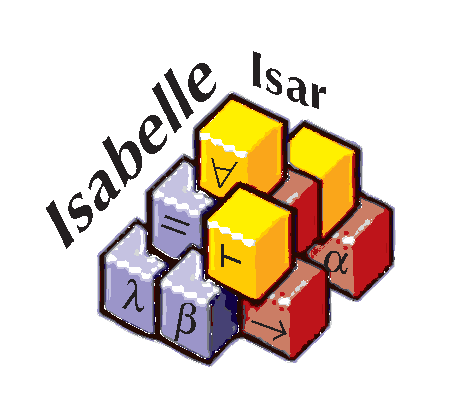
\includegraphics[scale=0.5]{isabelle_isar} \\[4ex] The Isabelle/Isar Reference Manual}
\author{\emph{Markus Wenzel} \\ TU M\"unchen}

\makeindex

\railterm{percent,ppercent,underscore,lbrace,rbrace,llbrace,rrbrace}
\railterm{ident,longident,symident,var,textvar,typefree,typevar,nat,string,verbatim,keyword}

\railalias{ident}{\railtoken{ident}}
\railalias{longident}{\railtoken{longident}}
\railalias{symident}{\railtoken{symident}}
\railalias{var}{\railtoken{var}}
\railalias{textvar}{\railtoken{textvar}}
\railalias{typefree}{\railtoken{typefree}}
\railalias{typevar}{\railtoken{typevar}}
\railalias{nat}{\railtoken{nat}}
\railalias{string}{\railtoken{string}}
\railalias{verbatim}{\railtoken{verbatim}}
\railalias{keyword}{\railtoken{keyword}}

\railalias{name}{\railqtoken{name}}
\railalias{nameref}{\railqtoken{nameref}}
\railalias{text}{\railqtoken{text}}
\railalias{type}{\railqtoken{type}}
\railalias{term}{\railqtoken{term}}
\railalias{prop}{\railqtoken{prop}}
\railalias{atom}{\railqtoken{atom}}

\newcommand{\drv}{\mathrel{\vdash}}
\newcommand{\edrv}{\mathop{\drv}\nolimits}
\newcommand{\Or}{\mathrel{\;|\;}}


\setcounter{secnumdepth}{2} \setcounter{tocdepth}{2}

\pagestyle{headings}
\sloppy
\binperiod     %%%treat . like a binary operator

\renewcommand{\phi}{\varphi}

%\includeonly{generic,refcard}


\begin{document}

\underscoreoff

\maketitle 

\begin{abstract}
  \emph{Intelligible semi-automated reasoning} (\emph{Isar}) is a generic
  approach to readable formal proof documents.  It sets out to bridge the
  semantic gap between any internal notions of proof based on primitive
  inferences and tactics, and an appropriate level of abstraction for
  user-level work.  The Isar formal proof language has been designed to
  satisfy quite contradictory requirements, being both ``declarative'' and
  immediately ``executable'', by virtue of the \emph{Isar/VM} interpreter.
  
  The current version of Isabelle offers Isar as an alternative proof language
  interface layer.  The Isabelle/Isar system provides an interpreter for the
  Isar formal proof language.  The input may consist either of proper document
  constructors, or improper auxiliary commands (for diagnostics, exploration
  etc.).  Proof texts consisting of proper elements only, admit a purely
  static reading, thus being intelligible later without requiring dynamic
  replay that is so typical for traditional proof scripts.  Any of the
  Isabelle/Isar commands may be executed in single-steps, so basically the
  interpreter has a proof text debugger already built-in.
  
  Employing the Isar instantiation of \emph{Proof~General}, a generic Emacs
  interface for interactive proof assistants, we arrive at a reasonable
  environment for \emph{live document editing}.  Thus proof texts may be
  developed incrementally by issuing proof commands, including forward and
  backward tracing of partial documents; intermediate states may be inspected
  by diagnostic commands.
  
  The Isar subsystem is tightly integrated into the Isabelle/Pure meta-logic
  implementation.  Theories, theorems, proof procedures etc.\ may be used
  interchangeably between classic Isabelle proof scripts and Isabelle/Isar
  documents.  Isar is as generic as Isabelle, able to support a wide range of
  object-logics.  Currently, the end-user working environment is most complete
  for Isabelle/HOL.
\end{abstract}

\pagenumbering{roman} \tableofcontents \clearfirst

%FIXME
% - HahnBanach paper
% - Freek Widijk's stuff

%FIXME
\nocite{Rudnicki:1992:MizarOverview}
\nocite{Harrison:1996:MizarHOL}
\nocite{Rudnicki:1992:MizarOverview}
\nocite{Trybulec:1993:MizarFeatures}
\nocite{Syme:1997:DECLARE}
\nocite{Syme:1998:thesis}
\nocite{Syme:1999:TPHOL}
\nocite{Zammit:1999:TPHOL}


\chapter{Introduction}

\section{Quick start}

Isar is already part of Isabelle (as of version Isabelle99, or later).  The
\texttt{isabelle} binary provides option \texttt{-I} to run the Isar
interaction loop at startup, rather than the plain ML top-level.  Thus the
quickest way to do anything with Isabelle/Isar is as follows:
\begin{ttbox}
isabelle -I HOL\medskip
\out{> Welcome to Isabelle/HOL (Isabelle99)}\medskip
theory Foo = Main:
constdefs foo :: nat  "foo == 1";
lemma "0 < foo" by (simp add: foo_def);
end
\end{ttbox}
Note that any Isabelle/Isar command may be retracted by \texttt{undo}.

Plain TTY-based interaction like this used to be quite feasible with
traditional tactic based theorem proving, but developing Isar documents
demands some better user-interface support.  \emph{Proof~General}\index{Proof
  General} of LFCS Edinburgh \cite{proofgeneral} offers a generic Emacs-based
environment for interactive theorem provers that does all the cut-and-paste
and forward-backward walk through the document in a very neat way.  Note that
in Isabelle/Isar, the current position within a partial proof document is more
informative than the actual proof state.  Thus Proof~General provides the
canonical working environment for Isabelle/Isar, both for getting acquainted
(e.g.\ by replaying existing Isar documents) and serious production work.

\medskip

The easiest way to use Proof~General is to make it the default Isabelle user
interface.  Just say something like this in your Isabelle settings file (cf.\ 
\cite{isabelle-sys}):
\begin{ttbox}
ISABELLE_INTERFACE=\$ISABELLE_HOME/contrib/ProofGeneral/isar/interface
PROOFGENERAL_OPTIONS=""
\end{ttbox}
You may have to change \texttt{\$ISABELLE_HOME/contrib/ProofGeneral} to the
actual installation directory of Proof~General.  From now on, the capital
\texttt{Isabelle} executable refers to the \texttt{ProofGeneral/isar}
interface.  Its usage is as follows:
\begin{ttbox}
Usage: interface [OPTIONS] [FILES ...]

  Options are:
    -l NAME      logic image name (default $ISABELLE_LOGIC=HOL)
    -p NAME      Emacs program name (default xemacs)
    -u BOOL      use .emacs file (default true)
    -w BOOL      use window system (default true)

  Starts Proof General for Isabelle/Isar with proof documents FILES
  (default Scratch.thy).

  PROOFGENERAL_OPTIONS=
\end{ttbox}
Apart from the command line, the defaults for these options may be overridden
via the \texttt{PROOFGENERAL_OPTIONS} setting as well.  For example, plain GNU
Emacs may be configured as follows:
\begin{ttbox}
PROOFGENERAL_OPTIONS="-p emacs"
\end{ttbox}

With the proper Isabelle interface setup, Isar documents may now be edited by
visiting appropriate theory files, e.g.\ 
\begin{ttbox}
Isabelle \({\langle}isabellehome{\rangle}\)/src/HOL/Isar_examples/BasicLogic.thy
\end{ttbox}
Users of XEmacs may note the tool bar for navigating forward and backward
through the text.  Consult the Proof~General documentation \cite{proofgeneral}
for further basic commands, such as \texttt{c-c return} or \texttt{c-c u}.

\medskip

Occasionally, a user's \texttt{.emacs} contains material that is incompatible
with the version of (X)Emacs that Proof~General prefers.  Then proper startup
may be still achieved by using the \texttt{-u false} option.\footnote{Also
  note that the Emacs lisp files
  \texttt{\$ISABELLE_HOME/etc/proofgeneral-settings.el} and
  \texttt{\$ISABELLE_HOME_USER/etc/proofgeneral-settings.el} are automatically
  loaded by Proof~General if invoked via the interface wrapper script.}


\section{How to write Isar proofs anyway?}

This is one of the key questions, of course.  Isar offers a rather different
approach to formal proof documents than plain old tactic scripts.  Experienced
users of existing interactive theorem proving systems may have to learn
thinking different in order to make effective use of Isabelle/Isar.  On the
other hand, Isabelle/Isar comes much closer to existing mathematical practice
of formal proof, so users with less experience in old-style tactical proving,
but a good understanding of mathematical proof might cope with Isar even
better.

Unfortunately, there is no tutorial on Isabelle/Isar available yet.  This
document really is a \emph{reference manual}.  Nevertheless, we will give some
discussions of the general principles underlying Isar in
chapter~\ref{ch:basics}, and provide some clues of how these may be put into
practice.  Some more background information on Isar is given in
\cite{Wenzel:1999:TPHOL}.  Furthermore, there are several examples distributed
with Isabelle (see directory \texttt{HOL/Isar_examples}).


%%% Local Variables: 
%%% mode: latex
%%% TeX-master: "isar-ref"
%%% End: 

\chapter{The Basics}

\section{Introduction}

This book is a tutorial on how to use the theorem prover Isabelle/HOL as a
specification and verification system. Isabelle is a generic system for
implementing logical formalisms, and Isabelle/HOL is the specialization
of Isabelle for HOL, which abbreviates Higher-Order Logic. We introduce
HOL step by step following the equation
\[ \mbox{HOL} = \mbox{Functional Programming} + \mbox{Logic}. \]
We do not assume that you are familiar with mathematical logic. 
However, we do assume that
you are used to logical and set theoretic notation, as covered
in a good discrete mathematics course~\cite{Rosen-DMA}, and
that you are familiar with the basic concepts of functional
programming~\cite{Bird-Haskell,Hudak-Haskell,paulson-ml2,Thompson-Haskell}.
Although this tutorial initially concentrates on functional programming, do
not be misled: HOL can express most mathematical concepts, and functional
programming is just one particularly simple and ubiquitous instance.

Isabelle~\cite{paulson-isa-book} is implemented in ML~\cite{SML}.  This has
influenced some of Isabelle/HOL's concrete syntax but is otherwise irrelevant
for us: this tutorial is based on
Isabelle/Isar~\cite{isabelle-isar-ref}, an extension of Isabelle which hides
the implementation language almost completely.  Thus the full name of the
system should be Isabelle/Isar/HOL, but that is a bit of a mouthful.

There are other implementations of HOL, in particular the one by Mike Gordon
\index{Gordon, Mike}%
\emph{et al.}, which is usually referred to as ``the HOL system''
\cite{mgordon-hol}. For us, HOL refers to the logical system, and sometimes
its incarnation Isabelle/HOL\@.

A tutorial is by definition incomplete.  Currently the tutorial only
introduces the rudiments of Isar's proof language. To fully exploit the power
of Isar, in particular the ability to write readable and structured proofs,
you need to consult the Isabelle/Isar Reference
Manual~\cite{isabelle-isar-ref} and Wenzel's PhD thesis~\cite{Wenzel-PhD}
which discusses many proof patterns. If you want to use Isabelle's ML level
directly (for example for writing your own proof procedures) see the Isabelle
Reference Manual~\cite{isabelle-ref}; for details relating to HOL see the
Isabelle/HOL manual~\cite{isabelle-HOL}. All manuals have a comprehensive
index.

\section{Theories}
\label{sec:Basic:Theories}

\index{theories|(}%
Working with Isabelle means creating theories. Roughly speaking, a
\textbf{theory} is a named collection of types, functions, and theorems,
much like a module in a programming language or a specification in a
specification language. In fact, theories in HOL can be either. The general
format of a theory \texttt{T} is
\begin{ttbox}
theory T
imports B\(@1\) \(\ldots\) B\(@n\)
begin
{\rmfamily\textit{declarations, definitions, and proofs}}
end
\end{ttbox}\cmmdx{theory}\cmmdx{imports}
where \texttt{B}$@1$ \dots\ \texttt{B}$@n$ are the names of existing
theories that \texttt{T} is based on and \textit{declarations,
    definitions, and proofs} represents the newly introduced concepts
(types, functions etc.) and proofs about them. The \texttt{B}$@i$ are the
direct \textbf{parent theories}\indexbold{parent theories} of~\texttt{T}\@.
Everything defined in the parent theories (and their parents, recursively) is
automatically visible. To avoid name clashes, identifiers can be
\textbf{qualified}\indexbold{identifiers!qualified}
by theory names as in \texttt{T.f} and~\texttt{B.f}. 
Each theory \texttt{T} must
reside in a \textbf{theory file}\index{theory files} named \texttt{T.thy}.

This tutorial is concerned with introducing you to the different linguistic
constructs that can fill the \textit{declarations, definitions, and
    proofs} above.  A complete grammar of the basic
constructs is found in the Isabelle/Isar Reference
Manual~\cite{isabelle-isar-ref}.

HOL's theory collection is available online at
\begin{center}\small
    \url{http://isabelle.in.tum.de/library/HOL/}
\end{center}
and is recommended browsing. Note that most of the theories 
are based on classical Isabelle without the Isar extension. This means that
they look slightly different than the theories in this tutorial, and that all
proofs are in separate ML files.

\begin{warn}
  HOL contains a theory \thydx{Main}, the union of all the basic
  predefined theories like arithmetic, lists, sets, etc.  
  Unless you know what you are doing, always include \isa{Main}
  as a direct or indirect parent of all your theories.
\end{warn}
There is also a growing Library~\cite{HOL-Library}\index{Library}
of useful theories that are not part of \isa{Main} but can be included
among the parents of a theory and will then be loaded automatically.%
\index{theories|)}


\section{Types, Terms and Formulae}
\label{sec:TypesTermsForms}

Embedded in a theory are the types, terms and formulae of HOL\@. HOL is a typed
logic whose type system resembles that of functional programming languages
like ML or Haskell. Thus there are
\index{types|(}
\begin{description}
\item[base types,] 
in particular \tydx{bool}, the type of truth values,
and \tydx{nat}, the type of natural numbers.
\item[type constructors,]\index{type constructors}
 in particular \tydx{list}, the type of
lists, and \tydx{set}, the type of sets. Type constructors are written
postfix, e.g.\ \isa{(nat)list} is the type of lists whose elements are
natural numbers. Parentheses around single arguments can be dropped (as in
\isa{nat list}), multiple arguments are separated by commas (as in
\isa{(bool,nat)ty}).
\item[function types,]\index{function types}
denoted by \isasymFun\indexbold{$IsaFun@\isasymFun}.
  In HOL \isasymFun\ represents \emph{total} functions only. As is customary,
  \isa{$\tau@1$ \isasymFun~$\tau@2$ \isasymFun~$\tau@3$} means
  \isa{$\tau@1$ \isasymFun~($\tau@2$ \isasymFun~$\tau@3$)}. Isabelle also
  supports the notation \isa{[$\tau@1,\dots,\tau@n$] \isasymFun~$\tau$}
  which abbreviates \isa{$\tau@1$ \isasymFun~$\cdots$ \isasymFun~$\tau@n$
    \isasymFun~$\tau$}.
\item[type variables,]\index{type variables}\index{variables!type}
  denoted by \ttindexboldpos{'a}{$Isatype}, \isa{'b} etc., just like in ML\@. They give rise
  to polymorphic types like \isa{'a \isasymFun~'a}, the type of the identity
  function.
\end{description}
\begin{warn}
  Types are extremely important because they prevent us from writing
  nonsense.  Isabelle insists that all terms and formulae must be well-typed
  and will print an error message if a type mismatch is encountered. To
  reduce the amount of explicit type information that needs to be provided by
  the user, Isabelle infers the type of all variables automatically (this is
  called \bfindex{type inference}) and keeps quiet about it. Occasionally
  this may lead to misunderstandings between you and the system. If anything
  strange happens, we recommend that you set the flag\index{flags}
  \isa{show_types}\index{*show_types (flag)}.  
  Isabelle will then display type information
  that is usually suppressed.  Simply type
\begin{ttbox}
ML "set show_types"
\end{ttbox}

\noindent
This can be reversed by \texttt{ML "reset show_types"}. Various other flags,
which we introduce as we go along, can be set and reset in the same manner.%
\index{flags!setting and resetting}
\end{warn}%
\index{types|)}


\index{terms|(}
\textbf{Terms} are formed as in functional programming by
applying functions to arguments. If \isa{f} is a function of type
\isa{$\tau@1$ \isasymFun~$\tau@2$} and \isa{t} is a term of type
$\tau@1$ then \isa{f~t} is a term of type $\tau@2$. HOL also supports
infix functions like \isa{+} and some basic constructs from functional
programming, such as conditional expressions:
\begin{description}
\item[\isa{if $b$ then $t@1$ else $t@2$}]\index{*if expressions}
Here $b$ is of type \isa{bool} and $t@1$ and $t@2$ are of the same type.
\item[\isa{let $x$ = $t$ in $u$}]\index{*let expressions}
is equivalent to $u$ where all free occurrences of $x$ have been replaced by
$t$. For example,
\isa{let x = 0 in x+x} is equivalent to \isa{0+0}. Multiple bindings are separated
by semicolons: \isa{let $x@1$ = $t@1$;\dots; $x@n$ = $t@n$ in $u$}.
\item[\isa{case $e$ of $c@1$ \isasymFun~$e@1$ |~\dots~| $c@n$ \isasymFun~$e@n$}]
\index{*case expressions}
evaluates to $e@i$ if $e$ is of the form $c@i$.
\end{description}

Terms may also contain
\isasymlambda-abstractions.\index{lambda@$\lambda$ expressions}
For example,
\isa{\isasymlambda{}x.~x+1} is the function that takes an argument \isa{x} and
returns \isa{x+1}. Instead of
\isa{\isasymlambda{}x.\isasymlambda{}y.\isasymlambda{}z.~$t$} we can write
\isa{\isasymlambda{}x~y~z.~$t$}.%
\index{terms|)}

\index{formulae|(}%
\textbf{Formulae} are terms of type \tydx{bool}.
There are the basic constants \cdx{True} and \cdx{False} and
the usual logical connectives (in decreasing order of priority):
\indexboldpos{\protect\isasymnot}{$HOL0not}, \indexboldpos{\protect\isasymand}{$HOL0and},
\indexboldpos{\protect\isasymor}{$HOL0or}, and \indexboldpos{\protect\isasymimp}{$HOL0imp},
all of which (except the unary \isasymnot) associate to the right. In
particular \isa{A \isasymimp~B \isasymimp~C} means \isa{A \isasymimp~(B
  \isasymimp~C)} and is thus logically equivalent to \isa{A \isasymand~B
  \isasymimp~C} (which is \isa{(A \isasymand~B) \isasymimp~C}).

Equality\index{equality} is available in the form of the infix function
\isa{=} of type \isa{'a \isasymFun~'a
  \isasymFun~bool}. Thus \isa{$t@1$ = $t@2$} is a formula provided $t@1$
and $t@2$ are terms of the same type. If $t@1$ and $t@2$ are of type
\isa{bool} then \isa{=} acts as \rmindex{if-and-only-if}.
The formula
\isa{$t@1$~\isasymnoteq~$t@2$} is merely an abbreviation for
\isa{\isasymnot($t@1$ = $t@2$)}.

Quantifiers\index{quantifiers} are written as
\isa{\isasymforall{}x.~$P$} and \isa{\isasymexists{}x.~$P$}. 
There is even
\isa{\isasymuniqex{}x.~$P$}, which
means that there exists exactly one \isa{x} that satisfies \isa{$P$}. 
Nested quantifications can be abbreviated:
\isa{\isasymforall{}x~y~z.~$P$} means
\isa{\isasymforall{}x.\isasymforall{}y.\isasymforall{}z.~$P$}.%
\index{formulae|)}

Despite type inference, it is sometimes necessary to attach explicit
\bfindex{type constraints} to a term.  The syntax is
\isa{$t$::$\tau$} as in \isa{x < (y::nat)}. Note that
\ttindexboldpos{::}{$Isatype} binds weakly and should therefore be enclosed
in parentheses.  For instance,
\isa{x < y::nat} is ill-typed because it is interpreted as
\isa{(x < y)::nat}.  Type constraints may be needed to disambiguate
expressions
involving overloaded functions such as~\isa{+}, 
\isa{*} and~\isa{<}.  Section~\ref{sec:overloading} 
discusses overloading, while Table~\ref{tab:overloading} presents the most
important overloaded function symbols.

In general, HOL's concrete \rmindex{syntax} tries to follow the conventions of
functional programming and mathematics.  Here are the main rules that you
should be familiar with to avoid certain syntactic traps:
\begin{itemize}
\item
Remember that \isa{f t u} means \isa{(f t) u} and not \isa{f(t u)}!
\item
Isabelle allows infix functions like \isa{+}. The prefix form of function
application binds more strongly than anything else and hence \isa{f~x + y}
means \isa{(f~x)~+~y} and not \isa{f(x+y)}.
\item Remember that in HOL if-and-only-if is expressed using equality.  But
  equality has a high priority, as befitting a relation, while if-and-only-if
  typically has the lowest priority.  Thus, \isa{\isasymnot~\isasymnot~P =
    P} means \isa{\isasymnot\isasymnot(P = P)} and not
  \isa{(\isasymnot\isasymnot P) = P}. When using \isa{=} to mean
  logical equivalence, enclose both operands in parentheses, as in \isa{(A
    \isasymand~B) = (B \isasymand~A)}.
\item
Constructs with an opening but without a closing delimiter bind very weakly
and should therefore be enclosed in parentheses if they appear in subterms, as
in \isa{(\isasymlambda{}x.~x) = f}.  This includes 
\isa{if},\index{*if expressions}
\isa{let},\index{*let expressions}
\isa{case},\index{*case expressions}
\isa{\isasymlambda}, and quantifiers.
\item
Never write \isa{\isasymlambda{}x.x} or \isa{\isasymforall{}x.x=x}
because \isa{x.x} is always taken as a single qualified identifier. Write
\isa{\isasymlambda{}x.~x} and \isa{\isasymforall{}x.~x=x} instead.
\item Identifiers\indexbold{identifiers} may contain the characters \isa{_} 
and~\isa{'}, except at the beginning.
\end{itemize}

For the sake of readability, we use the usual mathematical symbols throughout
the tutorial. Their \textsc{ascii}-equivalents are shown in table~\ref{tab:ascii} in
the appendix.

\begin{warn}
A particular
problem for novices can be the priority of operators. If you are unsure, use
additional parentheses. In those cases where Isabelle echoes your
input, you can see which parentheses are dropped --- they were superfluous. If
you are unsure how to interpret Isabelle's output because you don't know
where the (dropped) parentheses go, set the flag\index{flags}
\isa{show_brackets}\index{*show_brackets (flag)}:
\begin{ttbox}
ML "set show_brackets"; \(\dots\); ML "reset show_brackets";
\end{ttbox}
\end{warn}


\section{Variables}
\label{sec:variables}
\index{variables|(}

Isabelle distinguishes free and bound variables, as is customary. Bound
variables are automatically renamed to avoid clashes with free variables. In
addition, Isabelle has a third kind of variable, called a \textbf{schematic
  variable}\index{variables!schematic} or \textbf{unknown}\index{unknowns}, 
which must have a~\isa{?} as its first character.  
Logically, an unknown is a free variable. But it may be
instantiated by another term during the proof process. For example, the
mathematical theorem $x = x$ is represented in Isabelle as \isa{?x = ?x},
which means that Isabelle can instantiate it arbitrarily. This is in contrast
to ordinary variables, which remain fixed. The programming language Prolog
calls unknowns {\em logical\/} variables.

Most of the time you can and should ignore unknowns and work with ordinary
variables. Just don't be surprised that after you have finished the proof of
a theorem, Isabelle will turn your free variables into unknowns.  It
indicates that Isabelle will automatically instantiate those unknowns
suitably when the theorem is used in some other proof.
Note that for readability we often drop the \isa{?}s when displaying a theorem.
\begin{warn}
  For historical reasons, Isabelle accepts \isa{?} as an ASCII representation
  of the \(\exists\) symbol.  However, the \isa{?} character must then be followed
  by a space, as in \isa{?~x. f(x) = 0}.  Otherwise, \isa{?x} is
  interpreted as a schematic variable.  The preferred ASCII representation of
  the \(\exists\) symbol is \isa{EX}\@. 
\end{warn}%
\index{variables|)}

\section{Interaction and Interfaces}

Interaction with Isabelle can either occur at the shell level or through more
advanced interfaces. To keep the tutorial independent of the interface, we
have phrased the description of the interaction in a neutral language. For
example, the phrase ``to abandon a proof'' means to type \isacommand{oops} at the
shell level, which is explained the first time the phrase is used. Other
interfaces perform the same act by cursor movements and/or mouse clicks.
Although shell-based interaction is quite feasible for the kind of proof
scripts currently presented in this tutorial, the recommended interface for
Isabelle/Isar is the Emacs-based \bfindex{Proof
  General}~\cite{proofgeneral,Aspinall:TACAS:2000}.

Some interfaces (including the shell level) offer special fonts with
mathematical symbols. For those that do not, remember that \textsc{ascii}-equivalents
are shown in table~\ref{tab:ascii} in the appendix.

Finally, a word about semicolons.\indexbold{$Isar@\texttt{;}} 
Commands may but need not be terminated by semicolons.
At the shell level it is advisable to use semicolons to enforce that a command
is executed immediately; otherwise Isabelle may wait for the next keyword
before it knows that the command is complete.


\section{Getting Started}

Assuming you have installed Isabelle, you start it by typing \texttt{isabelle
  -I HOL} in a shell window.\footnote{Simply executing \texttt{isabelle -I}
  starts the default logic, which usually is already \texttt{HOL}.  This is
  controlled by the \texttt{ISABELLE_LOGIC} setting, see \emph{The Isabelle
    System Manual} for more details.} This presents you with Isabelle's most
basic \textsc{ascii} interface.  In addition you need to open an editor window to
create theory files.  While you are developing a theory, we recommend that you
type each command into the file first and then enter it into Isabelle by
copy-and-paste, thus ensuring that you have a complete record of your theory.
As mentioned above, Proof General offers a much superior interface.
If you have installed Proof General, you can start it by typing \texttt{Isabelle}.


\chapter{Syntax primitives}

The rather generic framework of Isabelle/Isar syntax emerges from three main
syntactic categories: \emph{commands} of the top-level Isar engine (covering
theory and proof elements), \emph{methods} for general goal refinements
(analogous to traditional ``tactics''), and \emph{attributes} for operations
on facts (within a certain context).  Here we give a reference of basic
syntactic entities underlying Isabelle/Isar syntax in a bottom-up manner.
Concrete theory and proof language elements will be introduced later on.

\medskip

In order to get started with writing well-formed Isabelle/Isar documents, the
most important aspect to be noted is the difference of \emph{inner} versus
\emph{outer} syntax.  Inner syntax is that of Isabelle types and terms of the
logic, while outer syntax is that of Isabelle/Isar theory sources (including
proofs).  As a general rule, inner syntax entities may occur only as
\emph{atomic entities} within outer syntax.  For example, the string
\texttt{"x + y"} and identifier \texttt{z} are legal term specifications
within a theory, while \texttt{x + y} is not.

\begin{warn}
  Old-style Isabelle theories used to fake parts of the inner syntax of types,
  with rather complicated rules when quotes may be omitted.  Despite the minor
  drawback of requiring quotes more often, the syntax of Isabelle/Isar is
  somewhat simpler and more robust in that respect.
\end{warn}

Printed theory documents usually omit quotes to gain readability (this is a
matter of {\LaTeX} macro setup, say via \verb,\isabellestyle,, see also
\cite{isabelle-sys}).  Experienced users of Isabelle/Isar may easily
reconstruct the lost technical information, while mere readers need not care
about quotes at all.

\medskip

Isabelle/Isar input may contain any number of input termination characters
``\texttt{;}'' (semicolon) to separate commands explicitly.  This is
particularly useful in interactive shell sessions to make clear where the
current command is intended to end.  Otherwise, the interpreter loop will
continue to issue a secondary prompt ``\verb,#,'' until an end-of-command is
clearly recognized from the input syntax, e.g.\ encounter of the next command
keyword.

Advanced interfaces such as Proof~General \cite{proofgeneral} do not require
explicit semicolons, the amount of input text is determined automatically by
inspecting the present content of the Emacs text buffer.  In the printed
presentation of Isabelle/Isar documents semicolons are omitted altogether for
readability.

\begin{warn}
  Proof~General requires certain syntax classification tables in order to
  achieve properly synchronized interaction with the Isabelle/Isar process.
  These tables need to be consistent with the Isabelle version and particular
  logic image to be used in a running session (common object-logics may well
  change the outer syntax).  The standard setup should work correctly with any
  of the ``official'' logic images derived from Isabelle/HOL (including HOLCF
  etc.).  Users of alternative logics may need to tell Proof~General
  explicitly, e.g.\ by giving an option \verb,-k ZF, (in conjunction with
  \verb,-l ZF, to specify the default logic image).
\end{warn}

\section{Lexical matters}\label{sec:lex-syntax}

The Isabelle/Isar outer syntax provides token classes as presented below; most
of these coincide with the inner lexical syntax as presented in
\cite{isabelle-ref}.

\indexoutertoken{ident}\indexoutertoken{longident}\indexoutertoken{symident}
\indexoutertoken{nat}\indexoutertoken{var}\indexoutertoken{typefree}
\indexoutertoken{typevar}\indexoutertoken{string}\indexoutertoken{altstring}
\indexoutertoken{verbatim}
\begin{matharray}{rcl}
  ident & = & letter\,quasiletter^* \\
  longident & = & ident (\verb,.,ident)^+ \\
  symident & = & sym^+ ~|~ \verb,\<,ident\verb,>, \\
  nat & = & digit^+ \\
  var & = & ident ~|~ \verb,?,ident ~|~ \verb,?,ident\verb,.,nat \\
  typefree & = & \verb,',ident \\
  typevar & = & typefree ~|~ \verb,?,typefree ~|~ \verb,?,typefree\verb,.,nat \\
  string & = & \verb,", ~\dots~ \verb,", \\
  altstring & = & \backquote ~\dots~ \backquote \\
  verbatim & = & \verb,{*, ~\dots~ \verb,*}, \\[1ex]

  letter & = & latin ~|~ \verb,\<,latin\verb,>, ~|~ \verb,\<,latin\,latin\verb,>, ~|~ greek ~|~ \\
         &   & \verb,\<^isub>, ~|~ \verb,\<^isup>, \\
  quasiletter & = & letter ~|~ digit ~|~ \verb,_, ~|~ \verb,', \\
  latin & = & \verb,a, ~|~ \dots ~|~ \verb,z, ~|~ \verb,A, ~|~ \dots ~|~ \verb,Z, \\
  digit & = & \verb,0, ~|~ \dots ~|~ \verb,9, \\
  sym & = & \verb,!, ~|~ \verb,#, ~|~ \verb,$, ~|~ \verb,%, ~|~ \verb,&, ~|~  %$
   \verb,*, ~|~ \verb,+, ~|~ \verb,-, ~|~ \verb,/, ~|~ \\
  & & \verb,<, ~|~ \verb,=, ~|~ \verb,>, ~|~ \verb,?, ~|~ \texttt{\at} ~|~
  \verb,^, ~|~ \verb,_, ~|~ \verb,|, ~|~ \verb,~, \\
greek & = & \verb,\<alpha>, ~|~ \verb,\<beta>, ~|~ \verb,\<gamma>, ~|~ \verb,\<delta>, ~| \\
      &   & \verb,\<epsilon>, ~|~ \verb,\<zeta>, ~|~ \verb,\<eta>, ~|~ \verb,\<theta>, ~| \\
      &   & \verb,\<iota>, ~|~ \verb,\<kappa>, ~|~ \verb,\<mu>, ~|~ \verb,\<nu>, ~| \\
      &   & \verb,\<xi>, ~|~ \verb,\<pi>, ~|~ \verb,\<rho>, ~|~ \verb,\<sigma>, ~| \\
      &   & \verb,\<tau>, ~|~ \verb,\<upsilon>, ~|~ \verb,\<phi>, ~|~ \verb,\<psi>, ~| \\
      &   & \verb,\<omega>, ~|~ \verb,\<Gamma>, ~|~ \verb,\<Delta>, ~|~ \verb,\<Theta>, ~| \\
      &   & \verb,\<Lambda>, ~|~ \verb,\<Xi>, ~|~ \verb,\<Pi>, ~|~ \verb,\<Sigma>, ~| \\
      &   & \verb,\<Upsilon>, ~|~ \verb,\<Phi>, ~|~ \verb,\<Psi>, ~|~ \verb,\<Omega>, \\
\end{matharray}

The syntax of $string$ admits any characters, including newlines; ``\verb|"|''
(double-quote) and ``\verb|\|'' (backslash) need to be escaped by a backslash.
Alternative strings according to $altstring$ are analogous, using single
back-quotes instead.  The body of $verbatim$ may consist of any text not
containing ``\verb|*}|''; this allows convenient inclusion of quotes without
further escapes.  The greek letters do \emph{not} include \verb,\<lambda>,,
which is already used differently in the meta-logic.

Common mathematical symbols such as $\forall$ are represented in Isabelle as
\verb,\<forall>,.  There are infinitely many legal symbols like this, although
proper presentation is left to front-end tools such as {\LaTeX} or
Proof~General with the X-Symbol package.  A list of standard Isabelle symbols
that work well with these tools is given in \cite[appendix~A]{isabelle-sys}.

Comments take the form \texttt{(*~\dots~*)} and may be nested, although
user-interface tools may prevent this.  Note that \texttt{(*~\dots~*)}
indicate source comments only, which are stripped after lexical analysis of
the input.  The Isar document syntax also provides formal comments that are
considered as part of the text (see \S\ref{sec:comments}).

\begin{warn}
  Proof~General does not handle nested comments properly; it is also unable to
  keep \verb,(*,\,/\,\verb,{*, and \verb,*),\,/\,\verb,*}, apart, despite
  their rather different meaning.  These are inherent problems of Emacs
  legacy.  Users should not be overly aggressive about nesting or alternating
  these delimiters.
\end{warn}


\section{Common syntax entities}

Subsequently, we introduce several basic syntactic entities, such as names,
terms, and theorem specifications, which have been factored out of the actual
Isar language elements to be described later.

Note that some of the basic syntactic entities introduced below (e.g.\
\railqtok{name}) act much like tokens rather than plain nonterminals (e.g.\
\railnonterm{sort}), especially for the sake of error messages.  E.g.\ syntax
elements like $\CONSTS$ referring to \railqtok{name} or \railqtok{type} would
really report a missing name or type rather than any of the constituent
primitive tokens such as \railtok{ident} or \railtok{string}.


\subsection{Names}

Entity \railqtok{name} usually refers to any name of types, constants,
theorems etc.\ that are to be \emph{declared} or \emph{defined} (so qualified
identifiers are excluded here).  Quoted strings provide an escape for
non-identifier names or those ruled out by outer syntax keywords (e.g.\
\verb|"let"|).  Already existing objects are usually referenced by
\railqtok{nameref}.

\indexoutertoken{name}\indexoutertoken{parname}\indexoutertoken{nameref}
\indexoutertoken{int}
\begin{rail}
  name: ident | symident | string | nat
  ;
  parname: '(' name ')'
  ;
  nameref: name | longident
  ;
  int: nat | '-' nat
  ;
\end{rail}


\subsection{Comments}\label{sec:comments}

Large chunks of plain \railqtok{text} are usually given \railtok{verbatim},
i.e.\ enclosed in \verb|{*|~\dots~\verb|*}|.  For convenience, any of the
smaller text units conforming to \railqtok{nameref} are admitted as well.  A
marginal \railnonterm{comment} is of the form \texttt{--} \railqtok{text}.
Any number of these may occur within Isabelle/Isar commands.

\indexoutertoken{text}\indexouternonterm{comment}
\begin{rail}
  text: verbatim | nameref
  ;
  comment: '--' text
  ;
\end{rail}


\subsection{Type classes, sorts and arities}

Classes are specified by plain names.  Sorts have a very simple inner syntax,
which is either a single class name $c$ or a list $\{c@1, \dots, c@n\}$
referring to the intersection of these classes.  The syntax of type arities is
given directly at the outer level.

\railalias{subseteq}{\isasymsubseteq}
\railterm{subseteq}

\indexouternonterm{sort}\indexouternonterm{arity}
\indexouternonterm{classdecl}
\begin{rail}
  classdecl: name (('<' | subseteq) (nameref + ','))?
  ;
  sort: nameref
  ;
  arity: ('(' (sort + ',') ')')? sort
  ;
\end{rail}


\subsection{Types and terms}\label{sec:types-terms}

The actual inner Isabelle syntax, that of types and terms of the logic, is far
too sophisticated in order to be modelled explicitly at the outer theory
level.  Basically, any such entity has to be quoted to turn it into a single
token (the parsing and type-checking is performed internally later).  For
convenience, a slightly more liberal convention is adopted: quotes may be
omitted for any type or term that is already atomic at the outer level.  For
example, one may just write \texttt{x} instead of \texttt{"x"}.  Note that
symbolic identifiers (e.g.\ \texttt{++} or $\forall$) are available as well,
provided these have not been superseded by commands or other keywords already
(e.g.\ \texttt{=} or \texttt{+}).

\indexoutertoken{type}\indexoutertoken{term}\indexoutertoken{prop}
\begin{rail}
  type: nameref | typefree | typevar
  ;
  term: nameref | var
  ;
  prop: term
  ;
\end{rail}

Positional instantiations are indicated by giving a sequence of terms, or the
placeholder ``$\_$'' (underscore), which means to skip a position.

\indexoutertoken{inst}\indexoutertoken{insts}
\begin{rail}
  inst: underscore | term
  ;
  insts: (inst *)
  ;
\end{rail}

Type declarations and definitions usually refer to \railnonterm{typespec} on
the left-hand side.  This models basic type constructor application at the
outer syntax level.  Note that only plain postfix notation is available here,
but no infixes.

\indexouternonterm{typespec}
\begin{rail}
  typespec: (() | typefree | '(' ( typefree + ',' ) ')') name
  ;
\end{rail}


\subsection{Mixfix annotations}

Mixfix annotations specify concrete \emph{inner} syntax of Isabelle types and
terms.  Some commands such as $\TYPES$ (see \S\ref{sec:types-pure}) admit
infixes only, while $\CONSTS$ (see \S\ref{sec:consts}) and
$\isarkeyword{syntax}$ (see \S\ref{sec:syn-trans}) support the full range of
general mixfixes and binders.

\indexouternonterm{infix}\indexouternonterm{mixfix}\indexouternonterm{structmixfix}
\begin{rail}
  infix: '(' ('infix' | 'infixl' | 'infixr') string? nat ')'
  ;
  mixfix: infix | '(' string prios? nat? ')' | '(' 'binder' string prios? nat ')'
  ;
  structmixfix: mixfix | '(' 'structure' ')'
  ;

  prios: '[' (nat + ',') ']'
  ;
\end{rail}

Here the \railtok{string} specifications refer to the actual mixfix template
(see also \cite{isabelle-ref}), which may include literal text, spacing,
blocks, and arguments (denoted by ``$_$''); the special symbol \verb,\<index>,
(printed as ``\i'') represents an index argument that specifies an implicit
structure reference (see also \S\ref{sec:locale}).  Infix and binder
declarations provide common abbreviations for particular mixfix declarations.
So in practice, mixfix templates mostly degenerate to literal text for
concrete syntax, such as ``\verb,++,'' for an infix symbol, or ``\verb,++,\i''
for an infix of an implicit structure.



\subsection{Proof methods}\label{sec:syn-meth}

Proof methods are either basic ones, or expressions composed of
methods via ``\texttt{,}'' (sequential composition), ``\texttt{|}''
(alternative choices), ``\texttt{?}'' (try), ``\texttt{+}'' (repeat at
least once), ``\texttt{[$n$]}'' (restriction to first $n$ sub-goals,
default $n = 1$).  In practice, proof methods are usually just a comma
separated list of \railqtok{nameref}~\railnonterm{args}
specifications.  Note that parentheses may be dropped for single
method specifications (with no arguments).

\indexouternonterm{method}
\begin{rail}
  method: (nameref | '(' methods ')') (() | '?' | '+' | '[' nat? ']')
  ;
  methods: (nameref args | method) + (',' | '|')
  ;
\end{rail}

Proper Isar proof methods do \emph{not} admit arbitrary goal
addressing, but refer either to the first sub-goal or all sub-goals
uniformly.  The goal restriction operator ``\texttt{[$n$]}'' evaluates
a method expression within a sandbox consisting of the first $n$
sub-goals (which need to exist).  For example,
$simp_all\mbox{\tt[}3\mbox{\tt]}$ simplifies the first three
sub-goals, while $(rule~foo, simp_all)\mbox{\tt[]}$ simplifies all new
goals that emerge from applying rule $foo$ to the originally first
one.

Improper methods, notably tactic emulations, offer a separate
low-level goal addressing scheme as explicit argument to the
individual tactic being involved.  Here $[!]$ refers to all goals, and
$[n-]$ to all goals starting from $n$,

\indexouternonterm{goalspec}
\begin{rail}
  goalspec: '[' (nat '-' nat | nat '-' | nat | '!' ) ']'
  ;
\end{rail}


\subsection{Attributes and theorems}\label{sec:syn-att}

Attributes (and proof methods, see \S\ref{sec:syn-meth}) have their own
``semi-inner'' syntax, in the sense that input conforming to
\railnonterm{args} below is parsed by the attribute a second time.  The
attribute argument specifications may be any sequence of atomic entities
(identifiers, strings etc.), or properly bracketed argument lists.  Below
\railqtok{atom} refers to any atomic entity, including any \railtok{keyword}
conforming to \railtok{symident}.

\indexoutertoken{atom}\indexouternonterm{args}\indexouternonterm{attributes}
\begin{rail}
  atom: nameref | typefree | typevar | var | nat | keyword
  ;
  arg: atom | '(' args ')' | '[' args ']'
  ;
  args: arg *
  ;
  attributes: '[' (nameref args * ',') ']'
  ;
\end{rail}

Theorem specifications come in several flavors: \railnonterm{axmdecl} and
\railnonterm{thmdecl} usually refer to axioms, assumptions or results of goal
statements, while \railnonterm{thmdef} collects lists of existing theorems.
Existing theorems are given by \railnonterm{thmref} and \railnonterm{thmrefs},
the former requires an actual singleton result.  There are three forms of
theorem references: (1) named facts $a$, (2) selections from named facts $a(i,
j - k)$, or (3) literal fact propositions using $altstring$ syntax
$\backquote\phi\backquote$, (see also method $fact$ in
\S\ref{sec:pure-meth-att}).

Any kind of theorem specification may include lists of attributes both on the
left and right hand sides; attributes are applied to any immediately preceding
fact.  If names are omitted, the theorems are not stored within the theorem
database of the theory or proof context, but any given attributes are applied
nonetheless.

\indexouternonterm{axmdecl}\indexouternonterm{thmdecl}
\indexouternonterm{thmdef}\indexouternonterm{thmref}
\indexouternonterm{thmrefs}\indexouternonterm{selection}
\begin{rail}
  axmdecl: name attributes? ':'
  ;
  thmdecl: thmbind ':'
  ;
  thmdef: thmbind '='
  ;
  thmref: (nameref selection? | altstring) attributes?
  ;
  thmrefs: thmref +
  ;

  thmbind: name attributes | name | attributes
  ;
  selection: '(' ((nat | nat '-' nat?) + ',') ')'
  ;
\end{rail}


\subsection{Term patterns and declarations}\label{sec:term-decls}

Wherever explicit propositions (or term fragments) occur in a proof text,
casual binding of schematic term variables may be given specified via patterns
of the form ``$\ISS{p@1\;\dots}{p@n}$''.  There are separate versions
available for \railqtok{term}s and \railqtok{prop}s.  The latter provides a
$\CONCLNAME$ part with patterns referring the (atomic) conclusion of a rule.

\indexouternonterm{termpat}\indexouternonterm{proppat}
\begin{rail}
  termpat: '(' ('is' term +) ')'
  ;
  proppat: '(' ('is' prop +) ')'
  ;
\end{rail}

Declarations of local variables $x :: \tau$ and logical propositions $a :
\phi$ represent different views on the same principle of introducing a local
scope.  In practice, one may usually omit the typing of $vars$ (due to
type-inference), and the naming of propositions (due to implicit references of
current facts).  In any case, Isar proof elements usually admit to introduce
multiple such items simultaneously.

\indexouternonterm{vars}\indexouternonterm{props}
\begin{rail}
  vars: (name+) ('::' type)?
  ;
  props: thmdecl? (prop proppat? +)
  ;
\end{rail}

The treatment of multiple declarations corresponds to the complementary focus
of $vars$ versus $props$: in ``$x@1~\dots~x@n :: \tau$'' the typing refers to
all variables, while in $a\colon \phi@1~\dots~\phi@n$ the naming refers to all
propositions collectively.  Isar language elements that refer to $vars$ or
$props$ typically admit separate typings or namings via another level of
iteration, with explicit $\AND$ separators; e.g.\ see $\FIXNAME$ and
$\ASSUMENAME$ in \S\ref{sec:proof-context}.


\subsection{Antiquotations}\label{sec:antiq}

\begin{matharray}{rcl}
  theory & : & \isarantiq \\
  thm & : & \isarantiq \\
  prop & : & \isarantiq \\
  term & : & \isarantiq \\
  const & : & \isarantiq \\
  abbrev & : & \isarantiq \\
  typeof & : & \isarantiq \\
  typ & : & \isarantiq \\
  thm_style & : & \isarantiq \\
  term_style & : & \isarantiq \\
  text & : & \isarantiq \\
  goals & : & \isarantiq \\
  subgoals & : & \isarantiq \\
  prf & : & \isarantiq \\
  full_prf & : & \isarantiq \\
  ML & : & \isarantiq \\
  ML_type & : & \isarantiq \\
  ML_struct & : & \isarantiq \\
\end{matharray}

The text body of formal comments (see also \S\ref{sec:comments}) may contain
antiquotations of logical entities, such as theorems, terms and types, which
are to be presented in the final output produced by the Isabelle document
preparation system (see also \S\ref{sec:document-prep}).

Thus embedding of
``\texttt{{\at}{\ttlbrace}term~[show_types]~"f(x)~=~a~+~x"{\ttrbrace}}''
within a text block would cause
\isa{(f{\isasymColon}'a~{\isasymRightarrow}~'a)~(x{\isasymColon}'a)~=~(a{\isasymColon}'a)~+~x}
to appear in the final {\LaTeX} document.  Also note that theorem
antiquotations may involve attributes as well.  For example,
\texttt{{\at}{\ttlbrace}thm~sym~[no_vars]{\ttrbrace}} would print the
statement where all schematic variables have been replaced by fixed ones,
which are easier to read.

\indexisarant{theory}\indexisarant{thm}\indexisarant{prop}\indexisarant{term}\indexisarant{const}
\indexisarant{abbrev}\indexisarant{typeof}\indexisarant{typ}\indexisarant{thm-style}
\indexisarant{term-style}\indexisarant{text}\indexisarant{goals}
\indexisarant{subgoals}\indexisarant{prf}\indexisarant{full-prf}\indexisarant{ML}
\indexisarant{ML-type}\indexisarant{ML-struct}

\begin{rail}
  atsign lbrace antiquotation rbrace
  ;

  antiquotation:
    'theory' options name |
    'thm' options thmrefs |
    'prop' options prop |
    'term' options term |
    'const' options term |
    'abbrev' options term |
    'typeof' options term |
    'typ' options type |
    'thm\_style' options name thmref |
    'term\_style' options name term |
    'text' options name |
    'goals' options |
    'subgoals' options |
    'prf' options thmrefs |
    'full\_prf' options thmrefs |
    'ML' options name |
    'ML\_type' options name |
    'ML\_struct' options name
  ;
  options: '[' (option * ',') ']'
  ;
  option: name | name '=' name
  ;
\end{rail}

Note that the syntax of antiquotations may \emph{not} include source comments
\texttt{(*~\dots~*)} or verbatim text \verb|{*|~\dots~\verb|*}|.

\begin{descr}
  
\item [$\at\{theory~A\}$] prints the name $A$, which is guaranteed to
  refer to a valid ancestor theory in the current context.

\item [$\at\{thm~\vec a\}$] prints theorems $\vec a$. Note that attribute
  specifications may be included as well (see also \S\ref{sec:syn-att}); the
  $no_vars$ operation (see \S\ref{sec:misc-meth-att}) would be particularly
  useful to suppress printing of schematic variables.

\item [$\at\{prop~\phi\}$] prints a well-typed proposition $\phi$.

\item [$\at\{term~t\}$] prints a well-typed term $t$.

\item [$\at\{const~c\}$] prints a well-defined constant $c$.
  
\item [$\at\{abbrev~c\,\vec x\}$] prints a constant abbreviation
  $c\,\vec x \equiv rhs$ as defined in the current context.

\item [$\at\{typeof~t\}$] prints the type of a well-typed term $t$.

\item [$\at\{typ~\tau\}$] prints a well-formed type $\tau$.
  
\item [$\at\{thm_style~s~a\}$] prints theorem $a$, previously applying a style
  $s$ to it (see below).
  
\item [$\at\{term_style~s~t\}$] prints a well-typed term $t$ after applying a
  style $s$ to it (see below).

\item [$\at\{text~s\}$] prints uninterpreted source text $s$.  This is
  particularly useful to print portions of text according to the Isabelle
  {\LaTeX} output style, without demanding well-formedness (e.g.\ small pieces
  of terms that should not be parsed or type-checked yet).

\item [$\at\{goals\}$] prints the current \emph{dynamic} goal state.  This is
  mainly for support of tactic-emulation scripts within Isar --- presentation
  of goal states does not conform to actual human-readable proof documents.
  Please do not include goal states into document output unless you really
  know what you are doing!
  
\item [$\at\{subgoals\}$] is similar to $goals$, but does not print the main
  goal.
  
\item [$\at\{prf~\vec a\}$] prints the (compact) proof terms corresponding to
  the theorems $\vec a$. Note that this requires proof terms to be switched on
  for the current object logic (see the ``Proof terms'' section of the
  Isabelle reference manual for information on how to do this).
  
\item [$\at\{full_prf~\vec a\}$] is like $\at\{prf~\vec a\}$, but displays the
  full proof terms, i.e.\ also displays information omitted in the compact
  proof term, which is denoted by ``$_$'' placeholders there.
  
\item [$\at\{ML~s\}$, $\at\{ML_type~s\}$, and $\at\{ML_struct~s\}$] check text
  $s$ as ML value, type, and structure, respectively.  If successful, the
  source is displayed verbatim.

\end{descr}

\medskip

The following standard styles for use with $thm_style$ and $term_style$ are
available:

\begin{descr}
  
\item [$lhs$] extracts the first argument of any application form with at
  least two arguments -- typically meta-level or object-level equality, or any
  other binary relation.
  
\item [$rhs$] is like $lhs$, but extracts the second argument.
  
\item [$concl$] extracts the conclusion $C$ from a nested meta-level
  implication $A@1 \Imp \cdots A@n \Imp C$.
  
\item [$prem1$, \dots, $prem9$] extract premise number $1$, \dots, $9$,
  respectively, from a nested meta-level implication $A@1 \Imp \cdots A@n \Imp
  C$.

\end{descr}

\medskip

The following options are available to tune the output.  Note that most of
these coincide with ML flags of the same names (see also \cite{isabelle-ref}).
\begin{descr}
\item[$show_types = bool$ and $show_sorts = bool$] control printing of
  explicit type and sort constraints.
\item[$show_structs = bool$] controls printing of implicit structures.
\item[$long_names = bool$] forces names of types and constants etc.\ to be
  printed in their fully qualified internal form.
\item[$short_names = bool$] forces names of types and constants etc.\ to be
  printed unqualified.  Note that internalizing the output again in the
  current context may well yield a different result.
\item[$unique_names = bool$] determines whether the printed version of
  qualified names should be made sufficiently long to avoid overlap with names
  declared further back.  Set to $false$ for more concise output.
\item[$eta_contract = bool$] prints terms in $\eta$-contracted form.
\item[$display = bool$] indicates if the text is to be output as multi-line
  ``display material'', rather than a small piece of text without line breaks
  (which is the default).
\item[$breaks = bool$] controls line breaks in non-display material.
\item[$quotes = bool$] indicates if the output should be enclosed in double
  quotes.
\item[$mode = name$] adds $name$ to the print mode to be used for presentation
  (see also \cite{isabelle-ref}).  Note that the standard setup for {\LaTeX}
  output is already present by default, including the modes ``$latex$'',
  ``$xsymbols$'', ``$symbols$''.
\item[$margin = nat$ and $indent = nat$] change the margin or indentation for
  pretty printing of display material.
\item[$source = bool$] prints the source text of the antiquotation arguments,
  rather than the actual value.  Note that this does not affect
  well-formedness checks of $thm$, $term$, etc. (only the $text$ antiquotation
  admits arbitrary output).
\item[$goals_limit = nat$] determines the maximum number of goals to be
  printed.
\item[$locale = name$] specifies an alternative context used for evaluating
  and printing the subsequent argument.
\end{descr}

For boolean flags, ``$name = true$'' may be abbreviated as ``$name$''.  All of
the above flags are disabled by default, unless changed from ML.

\medskip Note that antiquotations do not only spare the author from tedious
typing of logical entities, but also achieve some degree of
consistency-checking of informal explanations with formal developments:
well-formedness of terms and types with respect to the current theory or proof
context is ensured here.


\subsection{Tagged commands}\label{sec:tags}

Each Isabelle/Isar command may be decorated by presentation tags:

\indexouternonterm{tags}
\begin{rail}
  tags: ( tag * )
  ;
  tag: '\%' (ident | string)
\end{rail}

The tags $theory$, $proof$, $ML$ are already pre-declared for certain classes
of commands:

\medskip

\begin{tabular}{ll}
  $theory$ & theory begin and end \\
  $proof$ & all proof commands \\
  $ML$ & all commands involving ML code \\
\end{tabular}

\medskip The Isabelle document preparation system (see also
\cite{isabelle-sys}) allows tagged command regions to be presented
specifically, e.g.\ to fold proof texts, or drop parts of the text completely.

For example ``$\BYNAME~\%invisible~(auto)$'' would cause that piece of proof
to be treated as $invisible$ instead of $proof$ (the default), which may be
either show or hidden depending on the document setup.  In contrast,
``$\BYNAME~\%visible~(auto)$'' would force this text to be shown invariably.

Explicit tag specifications within a proof apply to all subsequent commands of
the same level of nesting.  For example,
``$\PROOFNAME~\%visible~\dots\QEDNAME$'' would force the whole sub-proof to be
typeset as $visible$ (unless some of its parts are tagged differently).

%%% Local Variables:
%%% mode: latex
%%% TeX-master: "isar-ref"
%%% End:

%
\begin{isabellebody}%
\def\isabellecontext{pure}%
%
\isadelimtheory
\isanewline
\isanewline
%
\endisadelimtheory
%
\isatagtheory
\isacommand{theory}\isamarkupfalse%
\ pure\isanewline
\isakeyword{imports}\ Pure\isanewline
\isakeyword{begin}%
\endisatagtheory
{\isafoldtheory}%
%
\isadelimtheory
%
\endisadelimtheory
%
\isamarkupchapter{Basic language elements \label{ch:pure-syntax}%
}
\isamarkuptrue%
%
\isamarkupsection{Other commands%
}
\isamarkuptrue%
%
\isamarkupsubsection{Diagnostics%
}
\isamarkuptrue%
%
\begin{isamarkuptext}%
\begin{matharray}{rcl}
    \indexdef{}{command}{pr}\hypertarget{command.pr}{\hyperlink{command.pr}{\mbox{\isa{\isacommand{pr}}}}}\isa{{\isachardoublequote}\isactrlsup {\isacharasterisk}{\isachardoublequote}} & : & \isarkeep{\cdot} \\
    \indexdef{}{command}{thm}\hypertarget{command.thm}{\hyperlink{command.thm}{\mbox{\isa{\isacommand{thm}}}}}\isa{{\isachardoublequote}\isactrlsup {\isacharasterisk}{\isachardoublequote}} & : & \isarkeep{theory~|~proof} \\
    \indexdef{}{command}{term}\hypertarget{command.term}{\hyperlink{command.term}{\mbox{\isa{\isacommand{term}}}}}\isa{{\isachardoublequote}\isactrlsup {\isacharasterisk}{\isachardoublequote}} & : & \isarkeep{theory~|~proof} \\
    \indexdef{}{command}{prop}\hypertarget{command.prop}{\hyperlink{command.prop}{\mbox{\isa{\isacommand{prop}}}}}\isa{{\isachardoublequote}\isactrlsup {\isacharasterisk}{\isachardoublequote}} & : & \isarkeep{theory~|~proof} \\
    \indexdef{}{command}{typ}\hypertarget{command.typ}{\hyperlink{command.typ}{\mbox{\isa{\isacommand{typ}}}}}\isa{{\isachardoublequote}\isactrlsup {\isacharasterisk}{\isachardoublequote}} & : & \isarkeep{theory~|~proof} \\
    \indexdef{}{command}{prf}\hypertarget{command.prf}{\hyperlink{command.prf}{\mbox{\isa{\isacommand{prf}}}}}\isa{{\isachardoublequote}\isactrlsup {\isacharasterisk}{\isachardoublequote}} & : & \isarkeep{theory~|~proof} \\
    \indexdef{}{command}{full\_prf}\hypertarget{command.full-prf}{\hyperlink{command.full-prf}{\mbox{\isa{\isacommand{full{\isacharunderscore}prf}}}}}\isa{{\isachardoublequote}\isactrlsup {\isacharasterisk}{\isachardoublequote}} & : & \isarkeep{theory~|~proof} \\
  \end{matharray}

  These diagnostic commands assist interactive development.  Note that
  \hyperlink{command.undo}{\mbox{\isa{\isacommand{undo}}}} does not apply here, the theory or proof
  configuration is not changed.

  \begin{rail}
    'pr' modes? nat? (',' nat)?
    ;
    'thm' modes? thmrefs
    ;
    'term' modes? term
    ;
    'prop' modes? prop
    ;
    'typ' modes? type
    ;
    'prf' modes? thmrefs?
    ;
    'full\_prf' modes? thmrefs?
    ;

    modes: '(' (name + ) ')'
    ;
  \end{rail}

  \begin{descr}

  \item [\hyperlink{command.pr}{\mbox{\isa{\isacommand{pr}}}}~\isa{{\isachardoublequote}goals{\isacharcomma}\ prems{\isachardoublequote}}] prints the current
  proof state (if present), including the proof context, current facts
  and goals.  The optional limit arguments affect the number of goals
  and premises to be displayed, which is initially 10 for both.
  Omitting limit values leaves the current setting unchanged.

  \item [\hyperlink{command.thm}{\mbox{\isa{\isacommand{thm}}}}~\isa{{\isachardoublequote}a\isactrlsub {\isadigit{1}}\ {\isasymdots}\ a\isactrlsub n{\isachardoublequote}}] retrieves
  theorems from the current theory or proof context.  Note that any
  attributes included in the theorem specifications are applied to a
  temporary context derived from the current theory or proof; the
  result is discarded, i.e.\ attributes involved in \isa{{\isachardoublequote}a\isactrlsub {\isadigit{1}}{\isacharcomma}\ {\isasymdots}{\isacharcomma}\ a\isactrlsub n{\isachardoublequote}} do not have any permanent effect.

  \item [\hyperlink{command.term}{\mbox{\isa{\isacommand{term}}}}~\isa{t} and \hyperlink{command.prop}{\mbox{\isa{\isacommand{prop}}}}~\isa{{\isasymphi}}]
  read, type-check and print terms or propositions according to the
  current theory or proof context; the inferred type of \isa{t} is
  output as well.  Note that these commands are also useful in
  inspecting the current environment of term abbreviations.

  \item [\hyperlink{command.typ}{\mbox{\isa{\isacommand{typ}}}}~\isa{{\isasymtau}}] reads and prints types of the
  meta-logic according to the current theory or proof context.

  \item [\hyperlink{command.prf}{\mbox{\isa{\isacommand{prf}}}}] displays the (compact) proof term of the
  current proof state (if present), or of the given theorems. Note
  that this requires proof terms to be switched on for the current
  object logic (see the ``Proof terms'' section of the Isabelle
  reference manual for information on how to do this).

  \item [\hyperlink{command.full-prf}{\mbox{\isa{\isacommand{full{\isacharunderscore}prf}}}}] is like \hyperlink{command.prf}{\mbox{\isa{\isacommand{prf}}}}, but displays
  the full proof term, i.e.\ also displays information omitted in the
  compact proof term, which is denoted by ``\isa{{\isacharunderscore}}'' placeholders
  there.

  \end{descr}

  All of the diagnostic commands above admit a list of \isa{modes}
  to be specified, which is appended to the current print mode (see
  also \cite{isabelle-ref}).  Thus the output behavior may be modified
  according particular print mode features.  For example, \hyperlink{command.pr}{\mbox{\isa{\isacommand{pr}}}}~\isa{{\isachardoublequote}{\isacharparenleft}latex\ xsymbols\ symbols{\isacharparenright}{\isachardoublequote}} would print the current
  proof state with mathematical symbols and special characters
  represented in {\LaTeX} source, according to the Isabelle style
  \cite{isabelle-sys}.

  Note that antiquotations (cf.\ \secref{sec:antiq}) provide a more
  systematic way to include formal items into the printed text
  document.%
\end{isamarkuptext}%
\isamarkuptrue%
%
\isamarkupsubsection{Inspecting the context%
}
\isamarkuptrue%
%
\begin{isamarkuptext}%
\begin{matharray}{rcl}
    \indexdef{}{command}{print\_commands}\hypertarget{command.print-commands}{\hyperlink{command.print-commands}{\mbox{\isa{\isacommand{print{\isacharunderscore}commands}}}}}\isa{{\isachardoublequote}\isactrlsup {\isacharasterisk}{\isachardoublequote}} & : & \isarkeep{\cdot} \\
    \indexdef{}{command}{print\_theory}\hypertarget{command.print-theory}{\hyperlink{command.print-theory}{\mbox{\isa{\isacommand{print{\isacharunderscore}theory}}}}}\isa{{\isachardoublequote}\isactrlsup {\isacharasterisk}{\isachardoublequote}} & : & \isarkeep{theory~|~proof} \\
    \indexdef{}{command}{print\_syntax}\hypertarget{command.print-syntax}{\hyperlink{command.print-syntax}{\mbox{\isa{\isacommand{print{\isacharunderscore}syntax}}}}}\isa{{\isachardoublequote}\isactrlsup {\isacharasterisk}{\isachardoublequote}} & : & \isarkeep{theory~|~proof} \\
    \indexdef{}{command}{print\_methods}\hypertarget{command.print-methods}{\hyperlink{command.print-methods}{\mbox{\isa{\isacommand{print{\isacharunderscore}methods}}}}}\isa{{\isachardoublequote}\isactrlsup {\isacharasterisk}{\isachardoublequote}} & : & \isarkeep{theory~|~proof} \\
    \indexdef{}{command}{print\_attributes}\hypertarget{command.print-attributes}{\hyperlink{command.print-attributes}{\mbox{\isa{\isacommand{print{\isacharunderscore}attributes}}}}}\isa{{\isachardoublequote}\isactrlsup {\isacharasterisk}{\isachardoublequote}} & : & \isarkeep{theory~|~proof} \\
    \indexdef{}{command}{print\_theorems}\hypertarget{command.print-theorems}{\hyperlink{command.print-theorems}{\mbox{\isa{\isacommand{print{\isacharunderscore}theorems}}}}}\isa{{\isachardoublequote}\isactrlsup {\isacharasterisk}{\isachardoublequote}} & : & \isarkeep{theory~|~proof} \\
    \indexdef{}{command}{find\_theorems}\hypertarget{command.find-theorems}{\hyperlink{command.find-theorems}{\mbox{\isa{\isacommand{find{\isacharunderscore}theorems}}}}}\isa{{\isachardoublequote}\isactrlsup {\isacharasterisk}{\isachardoublequote}} & : & \isarkeep{theory~|~proof} \\
    \indexdef{}{command}{thm\_deps}\hypertarget{command.thm-deps}{\hyperlink{command.thm-deps}{\mbox{\isa{\isacommand{thm{\isacharunderscore}deps}}}}}\isa{{\isachardoublequote}\isactrlsup {\isacharasterisk}{\isachardoublequote}} & : & \isarkeep{theory~|~proof} \\
    \indexdef{}{command}{print\_facts}\hypertarget{command.print-facts}{\hyperlink{command.print-facts}{\mbox{\isa{\isacommand{print{\isacharunderscore}facts}}}}}\isa{{\isachardoublequote}\isactrlsup {\isacharasterisk}{\isachardoublequote}} & : & \isarkeep{proof} \\
    \indexdef{}{command}{print\_binds}\hypertarget{command.print-binds}{\hyperlink{command.print-binds}{\mbox{\isa{\isacommand{print{\isacharunderscore}binds}}}}}\isa{{\isachardoublequote}\isactrlsup {\isacharasterisk}{\isachardoublequote}} & : & \isarkeep{proof} \\
  \end{matharray}

  \begin{rail}
    'print\_theory' ( '!'?)
    ;

    'find\_theorems' (('(' (nat)? ('with\_dups')? ')')?) (criterion *)
    ;
    criterion: ('-'?) ('name' ':' nameref | 'intro' | 'elim' | 'dest' |
      'simp' ':' term | term)
    ;
    'thm\_deps' thmrefs
    ;
  \end{rail}

  These commands print certain parts of the theory and proof context.
  Note that there are some further ones available, such as for the set
  of rules declared for simplifications.

  \begin{descr}
  
  \item [\hyperlink{command.print-commands}{\mbox{\isa{\isacommand{print{\isacharunderscore}commands}}}}] prints Isabelle's outer theory
  syntax, including keywords and command.
  
  \item [\hyperlink{command.print-theory}{\mbox{\isa{\isacommand{print{\isacharunderscore}theory}}}}] prints the main logical content of
  the theory context; the ``\isa{{\isachardoublequote}{\isacharbang}{\isachardoublequote}}'' option indicates extra
  verbosity.

  \item [\hyperlink{command.print-syntax}{\mbox{\isa{\isacommand{print{\isacharunderscore}syntax}}}}] prints the inner syntax of types
  and terms, depending on the current context.  The output can be very
  verbose, including grammar tables and syntax translation rules.  See
  \cite[\S7, \S8]{isabelle-ref} for further information on Isabelle's
  inner syntax.
  
  \item [\hyperlink{command.print-methods}{\mbox{\isa{\isacommand{print{\isacharunderscore}methods}}}}] prints all proof methods
  available in the current theory context.
  
  \item [\hyperlink{command.print-attributes}{\mbox{\isa{\isacommand{print{\isacharunderscore}attributes}}}}] prints all attributes
  available in the current theory context.
  
  \item [\hyperlink{command.print-theorems}{\mbox{\isa{\isacommand{print{\isacharunderscore}theorems}}}}] prints theorems resulting from
  the last command.
  
  \item [\hyperlink{command.find-theorems}{\mbox{\isa{\isacommand{find{\isacharunderscore}theorems}}}}~\isa{criteria}] retrieves facts
  from the theory or proof context matching all of given search
  criteria.  The criterion \isa{{\isachardoublequote}name{\isacharcolon}\ p{\isachardoublequote}} selects all theorems
  whose fully qualified name matches pattern \isa{p}, which may
  contain ``\isa{{\isachardoublequote}{\isacharasterisk}{\isachardoublequote}}'' wildcards.  The criteria \isa{intro},
  \isa{elim}, and \isa{dest} select theorems that match the
  current goal as introduction, elimination or destruction rules,
  respectively.  The criterion \isa{{\isachardoublequote}simp{\isacharcolon}\ t{\isachardoublequote}} selects all rewrite
  rules whose left-hand side matches the given term.  The criterion
  term \isa{t} selects all theorems that contain the pattern \isa{t} -- as usual, patterns may contain occurrences of the dummy
  ``\isa{{\isacharunderscore}}'', schematic variables, and type constraints.
  
  Criteria can be preceded by ``\isa{{\isachardoublequote}{\isacharminus}{\isachardoublequote}}'' to select theorems that
  do \emph{not} match. Note that giving the empty list of criteria
  yields \emph{all} currently known facts.  An optional limit for the
  number of printed facts may be given; the default is 40.  By
  default, duplicates are removed from the search result. Use
  \isa{with{\isacharunderscore}dups} to display duplicates.
  
  \item [\hyperlink{command.thm-deps}{\mbox{\isa{\isacommand{thm{\isacharunderscore}deps}}}}~\isa{{\isachardoublequote}a\isactrlsub {\isadigit{1}}\ {\isasymdots}\ a\isactrlsub n{\isachardoublequote}}]
  visualizes dependencies of facts, using Isabelle's graph browser
  tool (see also \cite{isabelle-sys}).
  
  \item [\hyperlink{command.print-facts}{\mbox{\isa{\isacommand{print{\isacharunderscore}facts}}}}] prints all local facts of the
  current context, both named and unnamed ones.
  
  \item [\hyperlink{command.print-binds}{\mbox{\isa{\isacommand{print{\isacharunderscore}binds}}}}] prints all term abbreviations
  present in the context.

  \end{descr}%
\end{isamarkuptext}%
\isamarkuptrue%
%
\isamarkupsubsection{History commands \label{sec:history}%
}
\isamarkuptrue%
%
\begin{isamarkuptext}%
\begin{matharray}{rcl}
    \indexdef{}{command}{undo}\hypertarget{command.undo}{\hyperlink{command.undo}{\mbox{\isa{\isacommand{undo}}}}}^{{ * }{ * }} & : & \isarkeep{\cdot} \\
    \indexdef{}{command}{redo}\hypertarget{command.redo}{\hyperlink{command.redo}{\mbox{\isa{\isacommand{redo}}}}}^{{ * }{ * }} & : & \isarkeep{\cdot} \\
    \indexdef{}{command}{kill}\hypertarget{command.kill}{\hyperlink{command.kill}{\mbox{\isa{\isacommand{kill}}}}}^{{ * }{ * }} & : & \isarkeep{\cdot} \\
  \end{matharray}

  The Isabelle/Isar top-level maintains a two-stage history, for
  theory and proof state transformation.  Basically, any command can
  be undone using \hyperlink{command.undo}{\mbox{\isa{\isacommand{undo}}}}, excluding mere diagnostic
  elements.  Its effect may be revoked via \hyperlink{command.redo}{\mbox{\isa{\isacommand{redo}}}}, unless
  the corresponding \hyperlink{command.undo}{\mbox{\isa{\isacommand{undo}}}} step has crossed the beginning
  of a proof or theory.  The \hyperlink{command.kill}{\mbox{\isa{\isacommand{kill}}}} command aborts the
  current history node altogether, discontinuing a proof or even the
  whole theory.  This operation is \emph{not} undo-able.

  \begin{warn}
    History commands should never be used with user interfaces such as
    Proof~General \cite{proofgeneral,Aspinall:TACAS:2000}, which takes
    care of stepping forth and back itself.  Interfering by manual
    \hyperlink{command.undo}{\mbox{\isa{\isacommand{undo}}}}, \hyperlink{command.redo}{\mbox{\isa{\isacommand{redo}}}}, or even \hyperlink{command.kill}{\mbox{\isa{\isacommand{kill}}}}
    commands would quickly result in utter confusion.
  \end{warn}%
\end{isamarkuptext}%
\isamarkuptrue%
%
\isamarkupsubsection{System operations%
}
\isamarkuptrue%
%
\begin{isamarkuptext}%
\begin{matharray}{rcl}
    \indexdef{}{command}{cd}\hypertarget{command.cd}{\hyperlink{command.cd}{\mbox{\isa{\isacommand{cd}}}}}\isa{{\isachardoublequote}\isactrlsup {\isacharasterisk}{\isachardoublequote}} & : & \isarkeep{\cdot} \\
    \indexdef{}{command}{pwd}\hypertarget{command.pwd}{\hyperlink{command.pwd}{\mbox{\isa{\isacommand{pwd}}}}}\isa{{\isachardoublequote}\isactrlsup {\isacharasterisk}{\isachardoublequote}} & : & \isarkeep{\cdot} \\
    \indexdef{}{command}{use\_thy}\hypertarget{command.use-thy}{\hyperlink{command.use-thy}{\mbox{\isa{\isacommand{use{\isacharunderscore}thy}}}}}\isa{{\isachardoublequote}\isactrlsup {\isacharasterisk}{\isachardoublequote}} & : & \isarkeep{\cdot} \\
  \end{matharray}

  \begin{rail}
    ('cd' | 'use\_thy' | 'update\_thy') name
    ;
  \end{rail}

  \begin{descr}

  \item [\hyperlink{command.cd}{\mbox{\isa{\isacommand{cd}}}}~\isa{path}] changes the current directory
  of the Isabelle process.

  \item [\hyperlink{command.pwd}{\mbox{\isa{\isacommand{pwd}}}}] prints the current working directory.

  \item [\hyperlink{command.use-thy}{\mbox{\isa{\isacommand{use{\isacharunderscore}thy}}}}~\isa{A}] preload theory \isa{A}.
  These system commands are scarcely used when working interactively,
  since loading of theories is done automatically as required.

  \end{descr}%
\end{isamarkuptext}%
\isamarkuptrue%
%
\isadelimtheory
%
\endisadelimtheory
%
\isatagtheory
\isacommand{end}\isamarkupfalse%
%
\endisatagtheory
{\isafoldtheory}%
%
\isadelimtheory
%
\endisadelimtheory
\isanewline
\end{isabellebody}%
%%% Local Variables:
%%% mode: latex
%%% TeX-master: "root"
%%% End:

\chapter{Generic tools and packages}\label{ch:gen-tools}

\section{Theory specification commands}

\subsection{Derived specifications}

\indexisarcmd{axiomatization}
\indexisarcmd{definition}\indexisaratt{defn}
\indexisarcmd{abbreviation}
\indexisarcmd{const-syntax}
\begin{matharray}{rcll}
  \isarcmd{axiomatization} & : & \isarkeep{local{\dsh}theory} & (axiomatic!)\\
  \isarcmd{definition} & : & \isarkeep{local{\dsh}theory} \\
  defn & : & \isaratt \\
  \isarcmd{abbreviation} & : & \isarkeep{local{\dsh}theory} \\
  \isarcmd{const_syntax} & : & \isarkeep{local{\dsh}theory} \\
\end{matharray}

These specification mechanisms provide a slightly more abstract view
than the underlying primitives of $\CONSTS$, $\DEFS$ (see
\S\ref{sec:consts}), and $\isarkeyword{axioms}$ (see
\S\ref{sec:axms-thms}).  In particular, type-inference is commonly
available, and result names need not be given.

\begin{rail}
  'axiomatization' locale? consts? ('where' specs)?
  ;
  'definition' locale? (constdecl? constdef +)
  ;
  'abbreviation' locale? mode? (constdecl? prop +)
  ;
  'const\_syntax' locale? mode? (nameref mixfix +)
  ;

  consts: ((name ('::' type)? structmixfix? | vars) + 'and')
  ;
  specs: (thmdecl? props + 'and')
  ;
\end{rail}

\begin{descr}
  
\item $\isarkeyword{axiomatization} ~ c@1 \dots c@n ~
  \isarkeyword{where} ~ A@1 \dots A@m$ introduces several constants
  simultaneously and states axiomatic properties for these.  The
  constants are marked as being specified once and for all, which
  prevents additional specifications being issued later on.
  
  Note that axiomatic specifications are only appropriate when
  declaring a new logical system.  Normal applications should only use
  definitional mechanisms!

\item $\isarkeyword{definition}~c~\isarkeyword{where}~eq$ produces an
  internal definition $c \equiv t$ according to the specification
  given as $eq$, which is then turned into a proven fact.  The given
  proposition may deviate from internal meta-level equality according
  to the rewrite rules declared as $defn$ by the object-logic.  This
  typically covers object-level equality $x = t$ and equivalence $A
  \leftrightarrow B$.  Users normally need not change the $defn$
  setup.
  
  Definitions may be presented with explicit arguments on the LHS, as
  well as additional conditions, e.g.\ $f\;x\;y = t$ instead of $f
  \equiv \lambda x\;y. t$ and $y \not= 0 \Imp g\;x\;y = u$ instead of
  an unguarded $g \equiv \lambda x\;y. u$.
  
  Multiple definitions are processed consecutively; no overloading is
  supported here.
  
\item $\isarkeyword{abbreviation}~c~\isarkeyword{where}~eq$ introduces
  a syntactic constant which is associated with a certain term
  according to the meta-level equality $eq$.
  
  Abbreviations participate in the usual type-inference process, but
  are expanded before the logic ever sees them.  Pretty printing of
  terms involves higher-order rewriting with rules stemming from
  reverted abbreviations.  This needs some care to avoid overlapping
  or looping syntactic replacements!
  
  The optional $mode$ specification restricts output to a particular
  print mode; using ``$input$'' here achieves the effect of one-way
  abbreviations.  The mode may also include an ``$output$'' qualifier
  that affects the concrete syntax declared for abbreviations, cf.\ 
  $\isarkeyword{syntax}$ in \S\ref{sec:syn-trans}.
  
\item $\isarkeyword{const_syntax}~c~mx$ associates mixfix syntax with
  an existing constant $c$.  This is a robust interface to the
  underlying $\isarkeyword{syntax}$ primitive (\S\ref{sec:syn-trans}).
  Type declaration and internal syntactic representation of given
  constants is retrieved from the context.
  
\end{descr}

Any of these specifications support an optional target locale context
(cf.\ \S\ref{sec:locale}).  In the latter case, constants being
introduced depend on certain fixed parameters of the locale context;
the constant name is qualified by the locale base name.  A syntactic
abbreviation takes care for convenient input and output of such terms,
making the parameters implicit and using the original short name.
Outside the locale context, the specified entities are available in
generalized form, with the parameters being open to explicit
instantiation.


\subsection{Locales and local contexts}\label{sec:locale}

Locales are named local contexts, consisting of a list of declaration elements
that are modeled after the Isar proof context commands (cf.\
\S\ref{sec:proof-context}).


\subsubsection{Localized commands}

Existing locales may be augmented later on by adding new facts.  Note that the
actual context definition may not be changed!  Several theory commands that
produce facts in some way are available in ``localized'' versions, referring
to a named locale instead of the global theory context.

\indexouternonterm{locale}
\begin{rail}
  locale: '(' 'in' name ')'
  ;
\end{rail}

Emerging facts of localized commands are stored in two versions, both in the
target locale and the theory (after export).  The latter view produces a
qualified binding, using the locale name as a name space prefix.

For example, ``$\LEMMAS~(\IN~loc)~a = \vec b$'' retrieves facts $\vec b$ from
the locale context of $loc$ and augments its body by an appropriate
``$\isarkeyword{notes}$'' element (see below).  The exported view of $a$,
after discharging the locale context, is stored as $loc{.}a$ within the global
theory.  A localized goal ``$\LEMMANAME~(\IN~loc)~a:~\phi$'' works similarly,
only that the fact emerges through the subsequent proof, which may refer to
the full infrastructure of the locale context (covering local parameters with
typing and concrete syntax, assumptions, definitions etc.).  Most notably,
fact declarations of the locale are active during the proof as well (e.g.\ 
local $simp$ rules).

As a general principle, results exported from a locale context acquire
additional premises according to the specification.  Usually this is only a
single predicate according to the standard ``closed'' view of locale
specifications.


\subsubsection{Locale specifications}

\indexisarcmd{locale}\indexisarcmd{print-locale}\indexisarcmd{print-locales}
\begin{matharray}{rcl}
  \isarcmd{locale} & : & \isartrans{theory}{local{\dsh}theory} \\
  \isarcmd{print_locale}^* & : & \isarkeep{theory~|~proof} \\
  \isarcmd{print_locales}^* & : & \isarkeep{theory~|~proof} \\
  intro_locales & : & \isarmeth \\
  unfold_locales & : & \isarmeth \\
\end{matharray}

\indexouternonterm{contextexpr}\indexouternonterm{contextelem}
\indexisarelem{fixes}\indexisarelem{constrains}\indexisarelem{assumes}
\indexisarelem{defines}\indexisarelem{notes}\indexisarelem{includes}

\begin{rail}
  'locale' ('(open)')? name ('=' localeexpr)?
  ;
  'print\_locale' '!'? localeexpr
  ;
  localeexpr: ((contextexpr '+' (contextelem+)) | contextexpr | (contextelem+))
  ;

  contextexpr: nameref | '(' contextexpr ')' |
  (contextexpr (name mixfix? +)) | (contextexpr + '+')
  ;
  contextelem: fixes | constrains | assumes | defines | notes | includes
  ;
  fixes: 'fixes' ((name ('::' type)? structmixfix? | vars) + 'and')
  ;
  constrains: 'constrains' (name '::' type + 'and')
  ;
  assumes: 'assumes' (thmdecl? props + 'and')
  ;
  defines: 'defines' (thmdecl? prop proppat? + 'and')
  ;
  notes: 'notes' (thmdef? thmrefs + 'and')
  ;
  includes: 'includes' contextexpr
  ;
\end{rail}

\begin{descr}
  
\item [$\LOCALE~loc~=~import~+~body$] defines a new locale $loc$ as a context
  consisting of a certain view of existing locales ($import$) plus some
  additional elements ($body$).  Both $import$ and $body$ are optional; the
  degenerate form $\LOCALE~loc$ defines an empty locale, which may still be
  useful to collect declarations of facts later on.  Type-inference on locale
  expressions automatically takes care of the most general typing that the
  combined context elements may acquire.

  The $import$ consists of a structured context expression, consisting of
  references to existing locales, renamed contexts, or merged contexts.
  Renaming uses positional notation: $c~\vec x$ means that (a prefix of) the
  fixed parameters of context $c$ are named according to $\vec x$; a
  ``\texttt{_}'' (underscore) \indexisarthm{_@\texttt{_}} means to skip that
  position.  Renaming by default deletes existing syntax.  Optionally,
  new syntax may by specified with a mixfix annotation.  Note that the
  special syntax declared with ``$(structure)$'' (see below) is
  neither deleted nor can it be changed.
  Merging proceeds from left-to-right, suppressing any duplicates stemming
  from different paths through the import hierarchy.

  The $body$ consists of basic context elements, further context expressions
  may be included as well.

  \begin{descr}

  \item [$\FIXES{~x::\tau~(mx)}$] declares a local parameter of type $\tau$
    and mixfix annotation $mx$ (both are optional).  The special syntax
    declaration ``$(structure)$'' means that $x$ may be referenced
    implicitly in this context.

  \item [$\CONSTRAINS{~x::\tau}$] introduces a type constraint $\tau$
    on the local parameter $x$.

  \item [$\ASSUMES{a}{\vec\phi}$] introduces local premises, similar to
    $\ASSUMENAME$ within a proof (cf.\ \S\ref{sec:proof-context}).

  \item [$\DEFINES{a}{x \equiv t}$] defines a previously declared parameter.
    This is close to $\DEFNAME$ within a proof (cf.\
    \S\ref{sec:proof-context}), but $\DEFINESNAME$ takes an equational
    proposition instead of variable-term pair.  The left-hand side of the
    equation may have additional arguments, e.g.\ ``$\DEFINES{}{f~\vec x
      \equiv t}$''.

  \item [$\NOTES{a}{\vec b}$] reconsiders facts within a local context.  Most
    notably, this may include arbitrary declarations in any attribute
    specifications included here, e.g.\ a local $simp$ rule.

  \item [$\INCLUDES{c}$] copies the specified context in a statically scoped
    manner.  Only available in the long goal format of \S\ref{sec:goals}.

    In contrast, the initial $import$ specification of a locale expression
    maintains a dynamic relation to the locales being referenced (benefiting
    from any later fact declarations in the obvious manner).
  \end{descr}
  
  Note that ``$\IS{p}$'' patterns given in the syntax of $\ASSUMESNAME$ and
  $\DEFINESNAME$ above are illegal in locale definitions.  In the long goal
  format of \S\ref{sec:goals}, term bindings may be included as expected,
  though.
  
  \medskip By default, locale specifications are ``closed up'' by turning the
  given text into a predicate definition $loc_axioms$ and deriving the
  original assumptions as local lemmas (modulo local definitions).  The
  predicate statement covers only the newly specified assumptions, omitting
  the content of included locale expressions.  The full cumulative view is
  only provided on export, involving another predicate $loc$ that refers to
  the complete specification text.
  
  In any case, the predicate arguments are those locale parameters that
  actually occur in the respective piece of text.  Also note that these
  predicates operate at the meta-level in theory, but the locale packages
  attempts to internalize statements according to the object-logic setup
  (e.g.\ replacing $\Forall$ by $\forall$, and $\Imp$ by $\imp$ in HOL; see
  also \S\ref{sec:object-logic}).  Separate introduction rules
  $loc_axioms.intro$ and $loc.intro$ are declared as well.
  
  The $(open)$ option of a locale specification prevents both the current
  $loc_axioms$ and cumulative $loc$ predicate constructions.  Predicates are
  also omitted for empty specification texts.

\item [$\isarkeyword{print_locale}~import~+~body$] prints the specified locale
  expression in a flattened form.  The notable special case
  $\isarkeyword{print_locale}~loc$ just prints the contents of the named
  locale, but keep in mind that type-inference will normalize type variables
  according to the usual alphabetical order.  The command omits
  $\isarkeyword{notes}$ elements by default.  Use
  $\isarkeyword{print_locale}!$ to get them included.

\item [$\isarkeyword{print_locales}$] prints the names of all locales of the
  current theory.

\item [$intro_locales$ and $unfold_locales$] repeatedly expand
  all introduction rules of locale predicates of the theory.  While
  $intro_locales$ only applies the $loc.intro$ introduction rules and
  therefore does not decend to assumptions, $unfold_locales$ is more
  aggressive and applies $loc_axioms.intro$ as well.  Both methods are
  aware of locale specifications entailed by the context, both from
  target and $\isarkeyword{includes}$ statements, and from
  interpretations (see below).  New goals that are entailed by the
  current context are discharged automatically.

\end{descr}


\subsubsection{Interpretation of locales}

Locale expressions (more precisely, \emph{context expressions}) may be
instantiated, and the instantiated facts added to the current context.
This requires a proof of the instantiated specification and is called
\emph{locale interpretation}.  Interpretation is possible in theories
and locales
(command $\isarcmd{interpretation}$) and also in proof contexts
($\isarcmd{interpret}$).

\indexisarcmd{interpretation}\indexisarcmd{interpret}
\indexisarcmd{print-interps}
\begin{matharray}{rcl}
  \isarcmd{interpretation} & : & \isartrans{theory}{proof(prove)} \\
  \isarcmd{interpret} & : & \isartrans{proof(state) ~|~ proof(chain)}{proof(prove)} \\
  \isarcmd{print_interps}^* & : &  \isarkeep{theory~|~proof} \\
\end{matharray}

\indexouternonterm{interp}

\railalias{printinterps}{print\_interps}
\railterm{printinterps}

\begin{rail}
  'interpretation' (interp | name ('<' | subseteq) contextexp)
  ;
  'interpret' interp
  ;
  printinterps '!'? name
  ;
  interp: thmdecl? contextexpr ('[' (inst+) ']')?
  ;
\end{rail}


\begin{descr}

\item [$\isarcmd{interpretation}~expr~insts$]

  The first form of $\isarcmd{interpretation}$ interprets $expr$
  in the theory.  The instantiation is given as a list of
  terms $insts$ and is positional.
  All parameters must receive an instantiation term --- with the
  exception of defined parameters.  These are, if omitted, derived
  from the defining equation and other instantiations.  Use ``\_'' to
  omit an instantiation term.  Free variables are automatically
  generalized.

  The command generates proof obligations for the instantiated
  specifications (assumes and defines elements).  Once these are
  discharged by the user, instantiated facts are added to the theory in
  a post-processing phase.

  The command is aware of interpretations already active in the
  theory.  No proof obligations are generated for those, neither is
  post-processing applied to their facts.  This avoids duplication of
  interpreted facts, in particular.  Note that, in the case of a
  locale with import, parts of the interpretation may already be
  active.  The command will only generate proof obligations and add
  facts for new parts.

  The context expression may be preceded by a name and/or attributes.
  These take effect in the post-processing of facts.  The name is used
  to prefix fact names, for example to avoid accidental hiding of
  other facts.  Attributes are applied after attributes of the
  interpreted facts.

  Adding facts to locales has the
  effect of adding interpreted facts to the theory for all active
  interpretations also.  That is, interpretations dynamically
  participate in any facts added to locales.

\item [$\isarcmd{interpretation}~name~\subseteq~expr$]

  This form of the command interprets $expr$ in the locale $name$.  It
  requires a proof that the specification of $name$ implies the
  specification of $expr$.  As in the localized version of the theorem
  command, the proof is in the context of $name$.  After the proof
  obligation has been dischared, the facts of $expr$
  become part of locale $name$ as \emph{derived} context elements and
  are available when the context $name$ is subsequently entered.
  Note that, like import, this is dynamic: facts added to a locale
  part of $expr$ after interpretation become also available in
  $name$.  Like facts
  of renamed context elements, facts obtained by interpretation may be
  accessed by prefixing with the parameter renaming (where the parameters
  are separated by `\_').

  Unlike interpretation in theories, instantiation is confined to the
  renaming of parameters, which may be specified as part of the context
  expression $expr$.  Using defined parameters in $name$ one may
  achieve an effect similar to instantiation, though.

  Only specification fragments of $expr$ that are not already part of
  $name$ (be it imported, derived or a derived fragment of the import)
  are considered by interpretation.  This enables circular
  interpretations.

  If interpretations of $name$ exist in the current theory, the
  command adds interpretations for $expr$ as well, with the same
  prefix and attributes, although only for fragments of $expr$ that
  are not interpreted in the theory already.

\item [$\isarcmd{interpret}~expr~insts$]
  interprets $expr$ in the proof context and is otherwise similar to
  interpretation in theories.  Free variables in instantiations are not
  generalized, however.

\item [$\isarcmd{print_interps}~loc$]
  prints the interpretations of a particular locale $loc$ that are
  active in the current context, either theory or proof context.  The
  exclamation point argument triggers printing of
  \emph{witness} theorems justifying interpretations.  These are
  normally omitted from the output.

  
\end{descr}

\begin{warn}
  Since attributes are applied to interpreted theorems, interpretation
  may modify the current simpset and claset.  Take this into
  account when choosing attributes for local theorems.
\end{warn}

\begin{warn}
  An interpretation in a theory may subsume previous interpretations.
  This happens if the same specification fragment is interpreted twice
  and the instantiation of the second interpretation is more general
  than the interpretation of the first.  A warning
  is issued, since it is likely that these could have been generalized
  in the first place.  The locale package does not attempt to remove
  subsumed interpretations.  This situation is normally harmless, but
  note that $blast$ gets confused by the presence of multiple axclass
  instances of a rule.
\end{warn}


\subsection{Type classes}

A special case of locales are type classes.
Type classes
consist of a locale with \emph{exactly one} type variable
and an corresponding axclass.

\indexisarcmd{instance}\indexisarcmd{class}\indexisarcmd{print-classes}
\begin{matharray}{rcl}
  \isarcmd{class} & : & \isartrans{theory}{local{\dsh}theory} \\
  \isarcmd{instance} & : & \isartrans{theory}{proof(prove)} \\
  \isarcmd{print_classes}^* & : & \isarkeep{theory~|~proof} \\
\end{matharray}

\begin{rail}
  'class' name '=' classexpr
  ;
  'instance' (instarity | instsubsort)
  ;
  'print\_classes'
  ;

  classexpr: ((superclassexpr '+' (contextelem+)) | superclassexpr | (contextelem+))
  ;
  instarity: (axmdecl)? (nameref '::' arity + 'and') (axmdecl prop +)?
  ;
  instsubsort: nameref ('<' | subseteq) sort
  ;
  superclassexpr: nameref | (nameref '+' superclassexpr)
  ;
\end{rail}

\begin{descr}

\item [$\CLASS~c = superclasses~+~body$] defines a new class $c$,
  inheriting from $superclasses$. Simultaneously, a locale
  named $c$ is introduced, inheriting from the locales
  corresponding to $superclasses$; also, an axclass
  named $c$, inheriting from the axclasses corresponding to
  $superclasses$. $\FIXESNAME$ in $body$ are lifted
  to the theory toplevel, constraining
  the free type variable to sort $c$ and stripping local syntax.
  $\ASSUMESNAME$ in $body$ are also lifted, 
  constraining
  the free type variable to sort $c$.

\item [$\INSTANCE~a: \vec{arity}~\vec{defs}$]
  sets up a goal stating type arities.  The proof would usually
  proceed by $intro_classes$, and then establish the characteristic theorems
  of the type classes involved.
  The $defs$, if given, must correspond to the class parameters
  involved in the $arities$ and are introduces in the theory
  before proof. Name and attributes given after the $\INSTANCE$
  command refer to \emph{all} definitions as a whole.
  After finishing the proof, the theory will be
  augmented by a type signature declaration corresponding to the
  resulting theorems.
  Note that this $\isarcmd{instance}$ command is different
  from primitive axclass $\isarcmd{instance}$ (see \ref{sec:axclass}).
  
\item [$\INSTANCE~c \subseteq \vec{c}$] sets up a
  goal stating 
  the interpretation of the locale corresponding to $c$
  in the merge of all locales corresponding to $\vec{c}$.
  After finishing the proof, it is automatically lifted to
  prove the additional class relation $c \subseteq \vec{c}$.

\item [$\isarkeyword{print_classes}$] prints the names of all classes
  in the current theory.

\end{descr}


\subsection{Axiomatic type classes}\label{sec:axclass}

\indexisarcmd{axclass}\indexisarmeth{intro-classes}
\begin{matharray}{rcl}
  \isarcmd{axclass} & : & \isartrans{theory}{theory} \\
  \isarcmd{instance} & : & \isartrans{theory}{proof(prove)} \\
  intro_classes & : & \isarmeth \\
\end{matharray}

Axiomatic type classes are provided by Isabelle/Pure as a \emph{definitional}
interface to type classes (cf.~\S\ref{sec:classes}).  Thus any object logic
may make use of this light-weight mechanism of abstract theories
\cite{Wenzel:1997:TPHOL}.  There is also a tutorial on using axiomatic type
classes in Isabelle \cite{isabelle-axclass} that is part of the standard
Isabelle documentation.

\begin{rail}
  'axclass' classdecl (axmdecl prop +)
  ;
  'instance' (nameref ('<' | subseteq) nameref | nameref '::' arity)
  ;
\end{rail}

\begin{descr}
  
\item [$\AXCLASS~c \subseteq \vec c~~axms$] defines an axiomatic type class as
  the intersection of existing classes, with additional axioms holding.  Class
  axioms may not contain more than one type variable.  The class axioms (with
  implicit sort constraints added) are bound to the given names.  Furthermore
  a class introduction rule is generated (being bound as
  $c_class{\dtt}intro$); this rule is employed by method $intro_classes$ to
  support instantiation proofs of this class.
  
  The ``axioms'' are stored as theorems according to the given name
  specifications, adding the class name $c$ as name space prefix; the same
  facts are also stored collectively as $c_class{\dtt}axioms$.
  
\item [$\INSTANCE~c@1 \subseteq c@2$ and $\INSTANCE~t :: (\vec s)s$] setup a
  goal stating a class relation or type arity.  The proof would usually
  proceed by $intro_classes$, and then establish the characteristic theorems
  of the type classes involved.  After finishing the proof, the theory will be
  augmented by a type signature declaration corresponding to the resulting
  theorem.

\item [$intro_classes$] repeatedly expands all class introduction rules of
  this theory.  Note that this method usually needs not be named explicitly,
  as it is already included in the default proof step (of $\PROOFNAME$ etc.).
  In particular, instantiation of trivial (syntactic) classes may be performed
  by a single ``$\DDOT$'' proof step.

\end{descr}



\section{Derived proof schemes}

\subsection{Generalized elimination}\label{sec:obtain}

\indexisarcmd{obtain}\indexisarcmd{guess}
\begin{matharray}{rcl}
  \isarcmd{obtain} & : & \isartrans{proof(state)}{proof(prove)} \\
  \isarcmd{guess}^* & : & \isartrans{proof(state)}{proof(prove)} \\
\end{matharray}

Generalized elimination means that additional elements with certain properties
may be introduced in the current context, by virtue of a locally proven
``soundness statement''.  Technically speaking, the $\OBTAINNAME$ language
element is like a declaration of $\FIXNAME$ and $\ASSUMENAME$ (see also see
\S\ref{sec:proof-context}), together with a soundness proof of its additional
claim.  According to the nature of existential reasoning, assumptions get
eliminated from any result exported from the context later, provided that the
corresponding parameters do \emph{not} occur in the conclusion.

\begin{rail}
  'obtain' parname? (vars + 'and') 'where' (props + 'and')
  ;
  'guess' (vars + 'and')
  ;
\end{rail}

$\OBTAINNAME$ is defined as a derived Isar command as follows, where $\vec b$
shall refer to (optional) facts indicated for forward chaining.
\begin{matharray}{l}
  \langle facts~\vec b\rangle \\
  \OBTAIN{\vec x}{a}{\vec \phi}~~\langle proof\rangle \equiv {} \\[1ex]
  \quad \HAVE{}{\All{thesis} (\All{\vec x} \vec\phi \Imp thesis) \Imp thesis} \\
  \quad \PROOF{succeed} \\
  \qquad \FIX{thesis} \\
  \qquad \ASSUME{that~[intro?]}{\All{\vec x} \vec\phi \Imp thesis} \\
  \qquad \THUS{}{thesis} \\
  \quad\qquad \APPLY{-} \\
  \quad\qquad \USING{\vec b}~~\langle proof\rangle \\
  \quad \QED{} \\
  \quad \FIX{\vec x}~\ASSUMENAME^\ast~a\colon~\vec\phi \\
\end{matharray}

Typically, the soundness proof is relatively straight-forward, often just by
canonical automated tools such as ``$\BY{simp}$'' or ``$\BY{blast}$''.
Accordingly, the ``$that$'' reduction above is declared as simplification and
introduction rule.

In a sense, $\OBTAINNAME$ represents at the level of Isar proofs what would be
meta-logical existential quantifiers and conjunctions.  This concept has a
broad range of useful applications, ranging from plain elimination (or
introduction) of object-level existential and conjunctions, to elimination
over results of symbolic evaluation of recursive definitions, for example.
Also note that $\OBTAINNAME$ without parameters acts much like $\HAVENAME$,
where the result is treated as a genuine assumption.

An alternative name to be used instead of ``$that$'' above may be
given in parentheses.

\medskip

The improper variant $\isarkeyword{guess}$ is similar to $\OBTAINNAME$, but
derives the obtained statement from the course of reasoning!  The proof starts
with a fixed goal $thesis$.  The subsequent proof may refine this to anything
of the form like $\All{\vec x} \vec\phi \Imp thesis$, but must not introduce
new subgoals.  The final goal state is then used as reduction rule for the
obtain scheme described above.  Obtained parameters $\vec x$ are marked as
internal by default, which prevents the proof context from being polluted by
ad-hoc variables.  The variable names and type constraints given as arguments
for $\isarkeyword{guess}$ specify a prefix of obtained parameters explicitly
in the text.

It is important to note that the facts introduced by $\OBTAINNAME$ and
$\isarkeyword{guess}$ may not be polymorphic: any type-variables occurring
here are fixed in the present context!


\subsection{Calculational reasoning}\label{sec:calculation}

\indexisarcmd{also}\indexisarcmd{finally}
\indexisarcmd{moreover}\indexisarcmd{ultimately}
\indexisarcmd{print-trans-rules}
\indexisaratt{trans}\indexisaratt{sym}\indexisaratt{symmetric}
\begin{matharray}{rcl}
  \isarcmd{also} & : & \isartrans{proof(state)}{proof(state)} \\
  \isarcmd{finally} & : & \isartrans{proof(state)}{proof(chain)} \\
  \isarcmd{moreover} & : & \isartrans{proof(state)}{proof(state)} \\
  \isarcmd{ultimately} & : & \isartrans{proof(state)}{proof(chain)} \\
  \isarcmd{print_trans_rules}^* & : & \isarkeep{theory~|~proof} \\
  trans & : & \isaratt \\
  sym & : & \isaratt \\
  symmetric & : & \isaratt \\
\end{matharray}

Calculational proof is forward reasoning with implicit application of
transitivity rules (such those of $=$, $\leq$, $<$).  Isabelle/Isar maintains
an auxiliary register $calculation$\indexisarthm{calculation} for accumulating
results obtained by transitivity composed with the current result.  Command
$\ALSO$ updates $calculation$ involving $this$, while $\FINALLY$ exhibits the
final $calculation$ by forward chaining towards the next goal statement.  Both
commands require valid current facts, i.e.\ may occur only after commands that
produce theorems such as $\ASSUMENAME$, $\NOTENAME$, or some finished proof of
$\HAVENAME$, $\SHOWNAME$ etc.  The $\MOREOVER$ and $\ULTIMATELY$ commands are
similar to $\ALSO$ and $\FINALLY$, but only collect further results in
$calculation$ without applying any rules yet.

Also note that the implicit term abbreviation ``$\dots$'' has its canonical
application with calculational proofs.  It refers to the argument of the
preceding statement. (The argument of a curried infix expression happens to be
its right-hand side.)

Isabelle/Isar calculations are implicitly subject to block structure in the
sense that new threads of calculational reasoning are commenced for any new
block (as opened by a local goal, for example).  This means that, apart from
being able to nest calculations, there is no separate \emph{begin-calculation}
command required.

\medskip

The Isar calculation proof commands may be defined as follows:\footnote{We
  suppress internal bookkeeping such as proper handling of block-structure.}
\begin{matharray}{rcl}
  \ALSO@0 & \equiv & \NOTE{calculation}{this} \\
  \ALSO@{n+1} & \equiv & \NOTE{calculation}{trans~[OF~calculation~this]} \\[0.5ex]
  \FINALLY & \equiv & \ALSO~\FROM{calculation} \\
  \MOREOVER & \equiv & \NOTE{calculation}{calculation~this} \\
  \ULTIMATELY & \equiv & \MOREOVER~\FROM{calculation} \\
\end{matharray}

\begin{rail}
  ('also' | 'finally') ('(' thmrefs ')')?
  ;
  'trans' (() | 'add' | 'del')
  ;
\end{rail}

\begin{descr}

\item [$\ALSO~(\vec a)$] maintains the auxiliary $calculation$ register as
  follows.  The first occurrence of $\ALSO$ in some calculational thread
  initializes $calculation$ by $this$. Any subsequent $\ALSO$ on the same
  level of block-structure updates $calculation$ by some transitivity rule
  applied to $calculation$ and $this$ (in that order).  Transitivity rules are
  picked from the current context, unless alternative rules are given as
  explicit arguments.

\item [$\FINALLY~(\vec a)$] maintaining $calculation$ in the same way as
  $\ALSO$, and concludes the current calculational thread.  The final result
  is exhibited as fact for forward chaining towards the next goal. Basically,
  $\FINALLY$ just abbreviates $\ALSO~\FROM{calculation}$.  Note that
  ``$\FINALLY~\SHOW{}{\Var{thesis}}~\DOT$'' and
  ``$\FINALLY~\HAVE{}{\phi}~\DOT$'' are typical idioms for concluding
  calculational proofs.

\item [$\MOREOVER$ and $\ULTIMATELY$] are analogous to $\ALSO$ and $\FINALLY$,
  but collect results only, without applying rules.

\item [$\isarkeyword{print_trans_rules}$] prints the list of transitivity
  rules (for calculational commands $\ALSO$ and $\FINALLY$) and symmetry rules
  (for the $symmetric$ operation and single step elimination patters) of the
  current context.

\item [$trans$] declares theorems as transitivity rules.

\item [$sym$] declares symmetry rules.

\item [$symmetric$] resolves a theorem with some rule declared as $sym$ in the
  current context.  For example, ``$\ASSUME{[symmetric]}{x = y}$'' produces a
  swapped fact derived from that assumption.

  In structured proof texts it is often more appropriate to use an explicit
  single-step elimination proof, such as ``$\ASSUME{}{x = y}~\HENCE{}{y =
    x}~\DDOT$''.  The very same rules known to $symmetric$ are declared as
  $elim?$ as well.

\end{descr}


\section{Proof tools}

\subsection{Miscellaneous methods and attributes}\label{sec:misc-meth-att}

\indexisarmeth{unfold}\indexisarmeth{fold}\indexisarmeth{insert}
\indexisarmeth{erule}\indexisarmeth{drule}\indexisarmeth{frule}
\indexisarmeth{fail}\indexisarmeth{succeed}
\begin{matharray}{rcl}
  unfold & : & \isarmeth \\
  fold & : & \isarmeth \\
  insert & : & \isarmeth \\[0.5ex]
  erule^* & : & \isarmeth \\
  drule^* & : & \isarmeth \\
  frule^* & : & \isarmeth \\
  succeed & : & \isarmeth \\
  fail & : & \isarmeth \\
\end{matharray}

\begin{rail}
  ('fold' | 'unfold' | 'insert') thmrefs
  ;
  ('erule' | 'drule' | 'frule') ('('nat')')? thmrefs
  ;
\end{rail}

\begin{descr}
  
\item [$unfold~\vec a$ and $fold~\vec a$] expand (or fold back again)
  the given definitions throughout all goals; any chained facts
  provided are inserted into the goal and subject to rewriting as
  well.

\item [$insert~\vec a$] inserts theorems as facts into all goals of the proof
  state.  Note that current facts indicated for forward chaining are ignored.

\item [$erule~\vec a$, $drule~\vec a$, and $frule~\vec a$] are similar to the
  basic $rule$ method (see \S\ref{sec:pure-meth-att}), but apply rules by
  elim-resolution, destruct-resolution, and forward-resolution, respectively
  \cite{isabelle-ref}.  The optional natural number argument (default $0$)
  specifies additional assumption steps to be performed here.

  Note that these methods are improper ones, mainly serving for
  experimentation and tactic script emulation.  Different modes of basic rule
  application are usually expressed in Isar at the proof language level,
  rather than via implicit proof state manipulations.  For example, a proper
  single-step elimination would be done using the plain $rule$ method, with
  forward chaining of current facts.

\item [$succeed$] yields a single (unchanged) result; it is the identity of
  the ``\texttt{,}'' method combinator (cf.\ \S\ref{sec:syn-meth}).

\item [$fail$] yields an empty result sequence; it is the identity of the
  ``\texttt{|}'' method combinator (cf.\ \S\ref{sec:syn-meth}).

\end{descr}

\indexisaratt{tagged}\indexisaratt{untagged}
\indexisaratt{THEN}\indexisaratt{COMP}
\indexisaratt{unfolded}\indexisaratt{folded}
\indexisaratt{standard}\indexisarattof{Pure}{elim-format}
\indexisaratt{no-vars}
\begin{matharray}{rcl}
  tagged & : & \isaratt \\
  untagged & : & \isaratt \\[0.5ex]
  THEN & : & \isaratt \\
  COMP & : & \isaratt \\[0.5ex]
  unfolded & : & \isaratt \\
  folded & : & \isaratt \\[0.5ex]
  elim_format & : & \isaratt \\
  standard^* & : & \isaratt \\
  no_vars^* & : & \isaratt \\
\end{matharray}

\begin{rail}
  'tagged' (nameref+)
  ;
  'untagged' name
  ;
  ('THEN' | 'COMP') ('[' nat ']')? thmref
  ;
  ('unfolded' | 'folded') thmrefs
  ;
\end{rail}

\begin{descr}

\item [$tagged~name~args$ and $untagged~name$] add and remove $tags$ of some
  theorem.  Tags may be any list of strings that serve as comment for some
  tools (e.g.\ $\LEMMANAME$ causes the tag ``$lemma$'' to be added to the
  result).  The first string is considered the tag name, the rest its
  arguments.  Note that untag removes any tags of the same name.

\item [$THEN~a$ and $COMP~a$] compose rules by resolution.  $THEN$ resolves
  with the first premise of $a$ (an alternative position may be also
  specified); the $COMP$ version skips the automatic lifting process that is
  normally intended (cf.\ \texttt{RS} and \texttt{COMP} in
  \cite[\S5]{isabelle-ref}).
  
\item [$unfolded~\vec a$ and $folded~\vec a$] expand and fold back
  again the given definitions throughout a rule.

\item [$elim_format$] turns a destruction rule into elimination rule format,
  by resolving with the rule $\PROP A \Imp (\PROP A \Imp \PROP B) \Imp \PROP
  B$.
  
  Note that the Classical Reasoner (\S\ref{sec:classical}) provides its own
  version of this operation.

\item [$standard$] puts a theorem into the standard form of object-rules at
  the outermost theory level.  Note that this operation violates the local
  proof context (including active locales).

\item [$no_vars$] replaces schematic variables by free ones; this is mainly
  for tuning output of pretty printed theorems.

\end{descr}


\subsection{Further tactic emulations}\label{sec:tactics}

The following improper proof methods emulate traditional tactics.  These admit
direct access to the goal state, which is normally considered harmful!  In
particular, this may involve both numbered goal addressing (default 1), and
dynamic instantiation within the scope of some subgoal.

\begin{warn}
  Dynamic instantiations refer to universally quantified parameters of
  a subgoal (the dynamic context) rather than fixed variables and term
  abbreviations of a (static) Isar context.
\end{warn}

Tactic emulation methods, unlike their ML counterparts, admit
simultaneous instantiation from both dynamic and static contexts.  If
names occur in both contexts goal parameters hide locally fixed
variables.  Likewise, schematic variables refer to term abbreviations,
if present in the static context.  Otherwise the schematic variable is
interpreted as a schematic variable and left to be solved by unification
with certain parts of the subgoal.

Note that the tactic emulation proof methods in Isabelle/Isar are consistently
named $foo_tac$.  Note also that variable names occurring on left hand sides
of instantiations must be preceded by a question mark if they coincide with
a keyword or contain dots.
This is consistent with the attribute $where$ (see \S\ref{sec:pure-meth-att}).

\indexisarmeth{rule-tac}\indexisarmeth{erule-tac}
\indexisarmeth{drule-tac}\indexisarmeth{frule-tac}
\indexisarmeth{cut-tac}\indexisarmeth{thin-tac}
\indexisarmeth{subgoal-tac}\indexisarmeth{rename-tac}
\indexisarmeth{rotate-tac}\indexisarmeth{tactic}
\begin{matharray}{rcl}
  rule_tac^* & : & \isarmeth \\
  erule_tac^* & : & \isarmeth \\
  drule_tac^* & : & \isarmeth \\
  frule_tac^* & : & \isarmeth \\
  cut_tac^* & : & \isarmeth \\
  thin_tac^* & : & \isarmeth \\
  subgoal_tac^* & : & \isarmeth \\
  rename_tac^* & : & \isarmeth \\
  rotate_tac^* & : & \isarmeth \\
  tactic^* & : & \isarmeth \\
\end{matharray}

\railalias{ruletac}{rule\_tac}
\railterm{ruletac}

\railalias{eruletac}{erule\_tac}
\railterm{eruletac}

\railalias{druletac}{drule\_tac}
\railterm{druletac}

\railalias{fruletac}{frule\_tac}
\railterm{fruletac}

\railalias{cuttac}{cut\_tac}
\railterm{cuttac}

\railalias{thintac}{thin\_tac}
\railterm{thintac}

\railalias{subgoaltac}{subgoal\_tac}
\railterm{subgoaltac}

\railalias{renametac}{rename\_tac}
\railterm{renametac}

\railalias{rotatetac}{rotate\_tac}
\railterm{rotatetac}

\begin{rail}
  ( ruletac | eruletac | druletac | fruletac | cuttac | thintac ) goalspec?
  ( insts thmref | thmrefs )
  ;
  subgoaltac goalspec? (prop +)
  ;
  renametac goalspec? (name +)
  ;
  rotatetac goalspec? int?
  ;
  'tactic' text
  ;

  insts: ((name '=' term) + 'and') 'in'
  ;
\end{rail}

\begin{descr}

\item [$rule_tac$ etc.] do resolution of rules with explicit instantiation.
  This works the same way as the ML tactics \texttt{res_inst_tac} etc. (see
  \cite[\S3]{isabelle-ref}).

  Multiple rules may be only given if there is no instantiation; then
  $rule_tac$ is the same as \texttt{resolve_tac} in ML (see
  \cite[\S3]{isabelle-ref}).

\item [$cut_tac$] inserts facts into the proof state as assumption of a
  subgoal, see also \texttt{cut_facts_tac} in \cite[\S3]{isabelle-ref}.  Note
  that the scope of schematic variables is spread over the main goal
  statement.  Instantiations may be given as well, see also ML tactic
  \texttt{cut_inst_tac} in \cite[\S3]{isabelle-ref}.

\item [$thin_tac~\phi$] deletes the specified assumption from a subgoal; note
  that $\phi$ may contain schematic variables.  See also \texttt{thin_tac} in
  \cite[\S3]{isabelle-ref}.

\item [$subgoal_tac~\phi$] adds $\phi$ as an assumption to a subgoal.  See
  also \texttt{subgoal_tac} and \texttt{subgoals_tac} in
  \cite[\S3]{isabelle-ref}.

\item [$rename_tac~\vec x$] renames parameters of a goal according to the list
  $\vec x$, which refers to the \emph{suffix} of variables.

\item [$rotate_tac~n$] rotates the assumptions of a goal by $n$ positions:
  from right to left if $n$ is positive, and from left to right if $n$ is
  negative; the default value is $1$.  See also \texttt{rotate_tac} in
  \cite[\S3]{isabelle-ref}.

\item [$tactic~text$] produces a proof method from any ML text of type
  \texttt{tactic}.  Apart from the usual ML environment and the current
  implicit theory context, the ML code may refer to the following locally
  bound values:

{\footnotesize\begin{verbatim}
val ctxt  : Proof.context
val facts : thm list
val thm   : string -> thm
val thms  : string -> thm list
\end{verbatim}}
  Here \texttt{ctxt} refers to the current proof context, \texttt{facts}
  indicates any current facts for forward-chaining, and
  \texttt{thm}~/~\texttt{thms} retrieve named facts (including global
  theorems) from the context.
\end{descr}


\subsection{The Simplifier}\label{sec:simplifier}

\subsubsection{Simplification methods}

\indexisarmeth{simp}\indexisarmeth{simp-all}
\begin{matharray}{rcl}
  simp & : & \isarmeth \\
  simp_all & : & \isarmeth \\
\end{matharray}

\indexouternonterm{simpmod}
\begin{rail}
  ('simp' | 'simp\_all') ('!' ?) opt? (simpmod *)
  ;

  opt: '(' ('no\_asm' | 'no\_asm\_simp' | 'no\_asm\_use' | 'asm\_lr' | 'depth\_limit' ':' nat) ')'
  ;
  simpmod: ('add' | 'del' | 'only' | 'cong' (() | 'add' | 'del') |
    'split' (() | 'add' | 'del')) ':' thmrefs
  ;
\end{rail}

\begin{descr}

\item [$simp$] invokes Isabelle's simplifier, after declaring additional rules
  according to the arguments given.  Note that the \railtterm{only} modifier
  first removes all other rewrite rules, congruences, and looper tactics
  (including splits), and then behaves like \railtterm{add}.

  \medskip The \railtterm{cong} modifiers add or delete Simplifier congruence
  rules (see also \cite{isabelle-ref}), the default is to add.

  \medskip The \railtterm{split} modifiers add or delete rules for the
  Splitter (see also \cite{isabelle-ref}), the default is to add.  This works
  only if the Simplifier method has been properly setup to include the
  Splitter (all major object logics such HOL, HOLCF, FOL, ZF do this already).

\item [$simp_all$] is similar to $simp$, but acts on all goals (backwards from
  the last to the first one).

\end{descr}

By default the Simplifier methods take local assumptions fully into account,
using equational assumptions in the subsequent normalization process, or
simplifying assumptions themselves (cf.\ \texttt{asm_full_simp_tac} in
\cite[\S10]{isabelle-ref}).  In structured proofs this is usually quite well
behaved in practice: just the local premises of the actual goal are involved,
additional facts may be inserted via explicit forward-chaining (using $\THEN$,
$\FROMNAME$ etc.).  The full context of assumptions is only included if the
``$!$'' (bang) argument is given, which should be used with some care, though.

Additional Simplifier options may be specified to tune the behavior further
(mostly for unstructured scripts with many accidental local facts):
``$(no_asm)$'' means assumptions are ignored completely (cf.\ 
\texttt{simp_tac}), ``$(no_asm_simp)$'' means assumptions are used in the
simplification of the conclusion but are not themselves simplified (cf.\ 
\texttt{asm_simp_tac}), and ``$(no_asm_use)$'' means assumptions are
simplified but are not used in the simplification of each other or the
conclusion (cf.\ \texttt{full_simp_tac}).  For compatibility reasons, there is
also an option ``$(asm_lr)$'', which means that an assumption is only used for
simplifying assumptions which are to the right of it (cf.\ 
\texttt{asm_lr_simp_tac}).  Giving an option ``$(depth_limit: n)$'' limits the
number of recursive invocations of the simplifier during conditional
rewriting.

\medskip

The Splitter package is usually configured to work as part of the Simplifier.
The effect of repeatedly applying \texttt{split_tac} can be simulated by
``$(simp~only\colon~split\colon~\vec a)$''.  There is also a separate $split$
method available for single-step case splitting.


\subsubsection{Declaring rules}

\indexisarcmd{print-simpset}
\indexisaratt{simp}\indexisaratt{split}\indexisaratt{cong}
\begin{matharray}{rcl}
  \isarcmd{print_simpset}^* & : & \isarkeep{theory~|~proof} \\
  simp & : & \isaratt \\
  cong & : & \isaratt \\
  split & : & \isaratt \\
\end{matharray}

\begin{rail}
  ('simp' | 'cong' | 'split') (() | 'add' | 'del')
  ;
\end{rail}

\begin{descr}

\item [$\isarcmd{print_simpset}$] prints the collection of rules declared to
  the Simplifier, which is also known as ``simpset'' internally
  \cite{isabelle-ref}.  This is a diagnostic command; $undo$ does not apply.

\item [$simp$] declares simplification rules.

\item [$cong$] declares congruence rules.

\item [$split$] declares case split rules.

\end{descr}


\subsubsection{Forward simplification}

\indexisaratt{simplified}
\begin{matharray}{rcl}
  simplified & : & \isaratt \\
\end{matharray}

\begin{rail}
  'simplified' opt? thmrefs?
  ;

  opt: '(' (noasm | noasmsimp | noasmuse) ')'
  ;
\end{rail}

\begin{descr}
  
\item [$simplified~\vec a$] causes a theorem to be simplified, either by
  exactly the specified rules $\vec a$, or the implicit Simplifier context if
  no arguments are given.  The result is fully simplified by default,
  including assumptions and conclusion; the options $no_asm$ etc.\ tune the
  Simplifier in the same way as the for the $simp$ method.

  Note that forward simplification restricts the simplifier to its most basic
  operation of term rewriting; solver and looper tactics \cite{isabelle-ref}
  are \emph{not} involved here.  The $simplified$ attribute should be only
  rarely required under normal circumstances.

\end{descr}


\subsubsection{Low-level equational reasoning}

\indexisarmeth{subst}\indexisarmeth{hypsubst}\indexisarmeth{split}
\begin{matharray}{rcl}
  subst^* & : & \isarmeth \\
  hypsubst^* & : & \isarmeth \\
  split^* & : & \isarmeth \\
\end{matharray}

\begin{rail}
  'subst' ('(' 'asm' ')')? ('(' (nat+) ')')? thmref
  ;
  'split' ('(' 'asm' ')')? thmrefs
  ;
\end{rail}

These methods provide low-level facilities for equational reasoning that are
intended for specialized applications only.  Normally, single step
calculations would be performed in a structured text (see also
\S\ref{sec:calculation}), while the Simplifier methods provide the canonical
way for automated normalization (see \S\ref{sec:simplifier}).

\begin{descr}

\item [$subst~eq$] performs a single substitution step using rule $eq$, which
  may be either a meta or object equality.

\item [$subst~(asm)~eq$] substitutes in an assumption.

\item [$subst~(i \dots j)~eq$] performs several substitutions in the
conclusion. The numbers $i$ to $j$ indicate the positions to substitute at.
Positions are ordered from the top of the term tree moving down from left to
right. For example, in $(a+b)+(c+d)$ there are three positions where
commutativity of $+$ is applicable: 1 refers to the whole term, 2 to $a+b$
and 3 to $c+d$. If the positions in the list $(i \dots j)$ are
non-overlapping (e.g. $(2~3)$ in $(a+b)+(c+d)$) you may assume all
substitutions are performed simultaneously. Otherwise the behaviour of
$subst$ is not specified.

\item [$subst~(asm)~(i \dots j)~eq$] performs the substitutions in the
assumptions. Positions $1 \dots i@1$ refer
to assumption 1, positions $i@1+1 \dots i@2$ to assumption 2, and so on.

\item [$hypsubst$] performs substitution using some assumption; this only
  works for equations of the form $x = t$ where $x$ is a free or bound
  variable.

\item [$split~\vec a$] performs single-step case splitting using rules $thms$.
  By default, splitting is performed in the conclusion of a goal; the $asm$
  option indicates to operate on assumptions instead.
  
  Note that the $simp$ method already involves repeated application of split
  rules as declared in the current context.
\end{descr}


\subsection{The Classical Reasoner}\label{sec:classical}

\subsubsection{Basic methods}

\indexisarmeth{rule}\indexisarmeth{default}\indexisarmeth{contradiction}
\indexisarmeth{intro}\indexisarmeth{elim}
\begin{matharray}{rcl}
  rule & : & \isarmeth \\
  contradiction & : & \isarmeth \\
  intro & : & \isarmeth \\
  elim & : & \isarmeth \\
\end{matharray}

\begin{rail}
  ('rule' | 'intro' | 'elim') thmrefs?
  ;
\end{rail}

\begin{descr}

\item [$rule$] as offered by the classical reasoner is a refinement over the
  primitive one (see \S\ref{sec:pure-meth-att}).  Both versions essentially
  work the same, but the classical version observes the classical rule context
  in addition to that of Isabelle/Pure.

  Common object logics (HOL, ZF, etc.) declare a rich collection of classical
  rules (even if these would qualify as intuitionistic ones), but only few
  declarations to the rule context of Isabelle/Pure
  (\S\ref{sec:pure-meth-att}).

\item [$contradiction$] solves some goal by contradiction, deriving any result
  from both $\lnot A$ and $A$.  Chained facts, which are guaranteed to
  participate, may appear in either order.

\item [$intro$ and $elim$] repeatedly refine some goal by intro- or
  elim-resolution, after having inserted any chained facts.  Exactly the rules
  given as arguments are taken into account; this allows fine-tuned
  decomposition of a proof problem, in contrast to common automated tools.

\end{descr}


\subsubsection{Automated methods}

\indexisarmeth{blast}\indexisarmeth{fast}\indexisarmeth{slow}
\indexisarmeth{best}\indexisarmeth{safe}\indexisarmeth{clarify}
\begin{matharray}{rcl}
  blast & : & \isarmeth \\
  fast & : & \isarmeth \\
  slow & : & \isarmeth \\
  best & : & \isarmeth \\
  safe & : & \isarmeth \\
  clarify & : & \isarmeth \\
\end{matharray}

\indexouternonterm{clamod}
\begin{rail}
  'blast' ('!' ?) nat? (clamod *)
  ;
  ('fast' | 'slow' | 'best' | 'safe' | 'clarify') ('!' ?) (clamod *)
  ;

  clamod: (('intro' | 'elim' | 'dest') ('!' | () | '?') | 'del') ':' thmrefs
  ;
\end{rail}

\begin{descr}
\item [$blast$] refers to the classical tableau prover (see \texttt{blast_tac}
  in \cite[\S11]{isabelle-ref}).  The optional argument specifies a
  user-supplied search bound (default 20).
\item [$fast$, $slow$, $best$, $safe$, and $clarify$] refer to the generic
  classical reasoner.  See \texttt{fast_tac}, \texttt{slow_tac},
  \texttt{best_tac}, \texttt{safe_tac}, and \texttt{clarify_tac} in
  \cite[\S11]{isabelle-ref} for more information.
\end{descr}

Any of the above methods support additional modifiers of the context of
classical rules.  Their semantics is analogous to the attributes given before.
Facts provided by forward chaining are inserted into the goal before
commencing proof search.  The ``!''~argument causes the full context of
assumptions to be included as well.


\subsubsection{Combined automated methods}\label{sec:clasimp}

\indexisarmeth{auto}\indexisarmeth{force}\indexisarmeth{clarsimp}
\indexisarmeth{fastsimp}\indexisarmeth{slowsimp}\indexisarmeth{bestsimp}
\begin{matharray}{rcl}
  auto & : & \isarmeth \\
  force & : & \isarmeth \\
  clarsimp & : & \isarmeth \\
  fastsimp & : & \isarmeth \\
  slowsimp & : & \isarmeth \\
  bestsimp & : & \isarmeth \\
\end{matharray}

\indexouternonterm{clasimpmod}
\begin{rail}
  'auto' '!'? (nat nat)? (clasimpmod *)
  ;
  ('force' | 'clarsimp' | 'fastsimp' | 'slowsimp' | 'bestsimp') '!'? (clasimpmod *)
  ;

  clasimpmod: ('simp' (() | 'add' | 'del' | 'only') |
    ('cong' | 'split') (() | 'add' | 'del') |
    'iff' (((() | 'add') '?'?) | 'del') |
    (('intro' | 'elim' | 'dest') ('!' | () | '?') | 'del')) ':' thmrefs
\end{rail}

\begin{descr}
\item [$auto$, $force$, $clarsimp$, $fastsimp$, $slowsimp$, and $bestsimp$]
  provide access to Isabelle's combined simplification and classical reasoning
  tactics.  These correspond to \texttt{auto_tac}, \texttt{force_tac},
  \texttt{clarsimp_tac}, and Classical Reasoner tactics with the Simplifier
  added as wrapper, see \cite[\S11]{isabelle-ref} for more information.  The
  modifier arguments correspond to those given in \S\ref{sec:simplifier} and
  \S\ref{sec:classical}.  Just note that the ones related to the Simplifier
  are prefixed by \railtterm{simp} here.

  Facts provided by forward chaining are inserted into the goal before doing
  the search.  The ``!''~argument causes the full context of assumptions to be
  included as well.
\end{descr}


\subsubsection{Declaring rules}

\indexisarcmd{print-claset}
\indexisaratt{intro}\indexisaratt{elim}\indexisaratt{dest}
\indexisaratt{iff}\indexisaratt{rule}
\begin{matharray}{rcl}
  \isarcmd{print_claset}^* & : & \isarkeep{theory~|~proof} \\
  intro & : & \isaratt \\
  elim & : & \isaratt \\
  dest & : & \isaratt \\
  rule & : & \isaratt \\
  iff & : & \isaratt \\
\end{matharray}

\begin{rail}
  ('intro' | 'elim' | 'dest') ('!' | () | '?') nat?
  ;
  'rule' 'del'
  ;
  'iff' (((() | 'add') '?'?) | 'del')
  ;
\end{rail}

\begin{descr}

\item [$\isarcmd{print_claset}$] prints the collection of rules declared to
  the Classical Reasoner, which is also known as ``simpset'' internally
  \cite{isabelle-ref}.  This is a diagnostic command; $undo$ does not apply.
  
\item [$intro$, $elim$, and $dest$] declare introduction, elimination, and
  destruction rules, respectively.  By default, rules are considered as
  \emph{unsafe} (i.e.\ not applied blindly without backtracking), while a
  single ``!'' classifies as \emph{safe}.  Rule declarations marked by ``?''
  coincide with those of Isabelle/Pure, cf.\ \S\ref{sec:pure-meth-att} (i.e.\ 
  are only applied in single steps of the $rule$ method).  The optional
  natural number specifies an explicit weight argument, which is ignored by
  automated tools, but determines the search order of single rule steps.

\item [$rule~del$] deletes introduction, elimination, or destruction rules from
  the context.

\item [$iff$] declares logical equivalences to the Simplifier and the
  Classical reasoner at the same time.  Non-conditional rules result in a
  ``safe'' introduction and elimination pair; conditional ones are considered
  ``unsafe''.  Rules with negative conclusion are automatically inverted
  (using $\lnot$ elimination internally).

  The ``?'' version of $iff$ declares rules to the Isabelle/Pure context only,
  and omits the Simplifier declaration.

\end{descr}


\subsubsection{Classical operations}

\indexisaratt{swapped}

\begin{matharray}{rcl}
  swapped & : & \isaratt \\
\end{matharray}

\begin{descr}

\item [$swapped$] turns an introduction rule into an elimination, by resolving
  with the classical swap principle $(\lnot B \Imp A) \Imp (\lnot A \Imp B)$.

\end{descr}


\subsection{Proof by cases and induction}\label{sec:cases-induct}

\subsubsection{Rule contexts}

\indexisarcmd{case}\indexisarcmd{print-cases}
\indexisaratt{case-names}\indexisaratt{case-conclusion}
\indexisaratt{params}\indexisaratt{consumes}
\begin{matharray}{rcl}
  \isarcmd{case} & : & \isartrans{proof(state)}{proof(state)} \\
  \isarcmd{print_cases}^* & : & \isarkeep{proof} \\
  case_names & : & \isaratt \\
  case_conclusion & : & \isaratt \\
  params & : & \isaratt \\
  consumes & : & \isaratt \\
\end{matharray}

The puristic way to build up Isar proof contexts is by explicit language
elements like $\FIXNAME$, $\ASSUMENAME$, $\LET$ (see
\S\ref{sec:proof-context}).  This is adequate for plain natural deduction, but
easily becomes unwieldy in concrete verification tasks, which typically
involve big induction rules with several cases.

The $\CASENAME$ command provides a shorthand to refer to a local context
symbolically: certain proof methods provide an environment of named ``cases''
of the form $c\colon \vec x, \vec \phi$; the effect of ``$\CASE{c}$'' is then
equivalent to ``$\FIX{\vec x}~\ASSUME{c}{\vec\phi}$''.  Term bindings may be
covered as well, notably $\Var{case}$ for the main conclusion.

By default, the ``terminology'' $\vec x$ of a case value is marked as hidden,
i.e.\ there is no way to refer to such parameters in the subsequent proof
text.  After all, original rule parameters stem from somewhere outside of the
current proof text.  By using the explicit form ``$\CASE{(c~\vec y)}$''
instead, the proof author is able to chose local names that fit nicely into
the current context.

\medskip

It is important to note that proper use of $\CASENAME$ does not provide means
to peek at the current goal state, which is not directly observable in Isar!
Nonetheless, goal refinement commands do provide named cases $goal@i$ for each
subgoal $i = 1, \dots, n$ of the resulting goal state.  Using this feature
requires great care, because some bits of the internal tactical machinery
intrude the proof text.  In particular, parameter names stemming from the
left-over of automated reasoning tools are usually quite unpredictable.

Under normal circumstances, the text of cases emerge from standard elimination
or induction rules, which in turn are derived from previous theory
specifications in a canonical way (say from $\isarkeyword{inductive}$
definitions).

\medskip Proper cases are only available if both the proof method and the
rules involved support this.  By using appropriate attributes, case names,
conclusions, and parameters may be also declared by hand.  Thus variant
versions of rules that have been derived manually become ready to use in
advanced case analysis later.

\begin{rail}
  'case' (caseref | '(' caseref ((name | underscore) +) ')')
  ;
  caseref: nameref attributes?
  ;

  'case\_names' (name +)
  ;
  'case\_conclusion' name (name *)
  ;
  'params' ((name *) + 'and')
  ;
  'consumes' nat?
  ;
\end{rail}

\begin{descr}
  
\item [$\CASE{(c~\vec x)}$] invokes a named local context $c\colon \vec x,
  \vec \phi$, as provided by an appropriate proof method (such as $cases$ and
  $induct$).  The command ``$\CASE{(c~\vec x)}$'' abbreviates ``$\FIX{\vec
    x}~\ASSUME{c}{\vec\phi}$''.

\item [$\isarkeyword{print_cases}$] prints all local contexts of the current
  state, using Isar proof language notation.  This is a diagnostic command;
  $undo$ does not apply.
  
\item [$case_names~\vec c$] declares names for the local contexts of premises
  of a theorem; $\vec c$ refers to the \emph{suffix} of the list of premises.
  
\item [$case_conclusion~c~\vec d$] declares names for the conclusions of a
  named premise $c$; here $\vec d$ refers to the prefix of arguments of a
  logical formula built by nesting a binary connective (e.g.\ $\lor$).
  
  Note that proof methods such as $induct$ and $coinduct$ already provide a
  default name for the conclusion as a whole.  The need to name subformulas
  only arises with cases that split into several sub-cases, as in common
  co-induction rules.

\item [$params~\vec p@1 \dots \vec p@n$] renames the innermost parameters of
  premises $1, \dots, n$ of some theorem.  An empty list of names may be given
  to skip positions, leaving the present parameters unchanged.
  
  Note that the default usage of case rules does \emph{not} directly expose
  parameters to the proof context.
  
\item [$consumes~n$] declares the number of ``major premises'' of a rule,
  i.e.\ the number of facts to be consumed when it is applied by an
  appropriate proof method.  The default value of $consumes$ is $n = 1$, which
  is appropriate for the usual kind of cases and induction rules for inductive
  sets (cf.\ \S\ref{sec:hol-inductive}).  Rules without any $consumes$
  declaration given are treated as if $consumes~0$ had been specified.
  
  Note that explicit $consumes$ declarations are only rarely needed; this is
  already taken care of automatically by the higher-level $cases$, $induct$,
  and $coinduct$ declarations.

\end{descr}


\subsubsection{Proof methods}

\indexisarmeth{cases}\indexisarmeth{induct}\indexisarmeth{coinduct}
\begin{matharray}{rcl}
  cases & : & \isarmeth \\
  induct & : & \isarmeth \\
  coinduct & : & \isarmeth \\
\end{matharray}

The $cases$, $induct$, and $coinduct$ methods provide a uniform interface to
common proof techniques over datatypes, inductive sets, recursive functions
etc.  The corresponding rules may be specified and instantiated in a casual
manner.  Furthermore, these methods provide named local contexts that may be
invoked via the $\CASENAME$ proof command within the subsequent proof text.
This accommodates compact proof texts even when reasoning about large
specifications.

The $induct$ method also provides some additional infrastructure in order to
be applicable to structure statements (either using explicit meta-level
connectives, or including facts and parameters separately).  This avoids
cumbersome encoding of ``strengthened'' inductive statements within the
object-logic.

\begin{rail}
  'cases' open? (insts * 'and') rule?
  ;
  'induct' open? (definsts * 'and') \\ fixing? taking? rule?
  ;
  'coinduct' open? insts taking rule?
  ;

  open: '(' 'open' ')'
  ;
  rule: ('type' | 'set') ':' (nameref +) | 'rule' ':' (thmref +)
  ;
  definst: name ('==' | equiv) term | inst
  ;
  definsts: ( definst *)
  ;
  fixing: 'fixing' ':' ((term *) 'and' +)
  ;
  taking: 'taking' ':' insts
  ;
\end{rail}

\begin{descr}

\item [$cases~insts~R$] applies method $rule$ with an appropriate case
  distinction theorem, instantiated to the subjects $insts$.  Symbolic case
  names are bound according to the rule's local contexts.

  The rule is determined as follows, according to the facts and arguments
  passed to the $cases$ method:
  \begin{matharray}{llll}
    \Text{facts}    &       & \Text{arguments} & \Text{rule} \\\hline
                    & cases &           & \Text{classical case split} \\
                    & cases & t         & \Text{datatype exhaustion (type of $t$)} \\
    \edrv a \in A   & cases & \dots     & \Text{inductive set elimination (of $A$)} \\
    \dots           & cases & \dots ~ R & \Text{explicit rule $R$} \\
  \end{matharray}

  Several instantiations may be given, referring to the \emph{suffix} of
  premises of the case rule; within each premise, the \emph{prefix} of
  variables is instantiated.  In most situations, only a single term needs to
  be specified; this refers to the first variable of the last premise (it is
  usually the same for all cases).

  The ``$(open)$'' option causes the parameters of the new local contexts to
  be exposed to the current proof context.  Thus local variables stemming from
  distant parts of the theory development may be introduced in an implicit
  manner, which can be quite confusing to the reader.  Furthermore, this
  option may cause unwanted hiding of existing local variables, resulting in
  less robust proof texts.

\item [$induct~insts~R$] is analogous to the $cases$ method, but refers to
  induction rules, which are determined as follows:
  \begin{matharray}{llll}
    \Text{facts}    &        & \Text{arguments} & \Text{rule} \\\hline
                    & induct & P ~ x ~ \dots & \Text{datatype induction (type of $x$)} \\
    \edrv x \in A   & induct & \dots         & \Text{set induction (of $A$)} \\
    \dots           & induct & \dots ~ R     & \Text{explicit rule $R$} \\
  \end{matharray}
  
  Several instantiations may be given, each referring to some part of
  a mutual inductive definition or datatype --- only related partial
  induction rules may be used together, though.  Any of the lists of
  terms $P, x, \dots$ refers to the \emph{suffix} of variables present
  in the induction rule.  This enables the writer to specify only
  induction variables, or both predicates and variables, for example.
  
  Instantiations may be definitional: equations $x \equiv t$ introduce local
  definitions, which are inserted into the claim and discharged after applying
  the induction rule.  Equalities reappear in the inductive cases, but have
  been transformed according to the induction principle being involved here.
  In order to achieve practically useful induction hypotheses, some variables
  occurring in $t$ need to be fixed (see below).
  
  The optional ``$fixing\colon \vec x$'' specification generalizes variables
  $\vec x$ of the original goal before applying induction.  Thus induction
  hypotheses may become sufficiently general to get the proof through.
  Together with definitional instantiations, one may effectively perform
  induction over expressions of a certain structure.
  
  The optional ``$taking\colon \vec t$'' specification provides additional
  instantiations of a prefix of pending variables in the rule.  Such schematic
  induction rules rarely occur in practice, though.

  The ``$(open)$'' option works the same way as for $cases$.

\item [$coinduct~inst~R$] is analogous to the $induct$ method, but refers to
  coinduction rules, which are determined as follows:
  \begin{matharray}{llll}
    \Text{goal}     &          & \Text{arguments} & \Text{rule} \\\hline
                    & coinduct & x ~ \dots        & \Text{type coinduction (type of $x$)} \\
    x \in A         & coinduct & \dots            & \Text{set coinduction (of $A$)} \\
    \dots           & coinduct & \dots ~ R        & \Text{explicit rule $R$} \\
  \end{matharray}
  
  Coinduction is the dual of induction.  Induction essentially eliminates $x
  \in A$ towards a generic result $P ~ x$, while coinduction introduces $x \in
  A$ starting with $x \in B$, for a suitable ``bisimulation'' $B$.  The cases
  of a coinduct rule are typically named after the sets being covered, while
  the conclusions consist of several alternatives being named after the
  individual destructor patterns.
  
  The given instantiation refers to the \emph{prefix} of variables occurring
  in the rule's conclusion.  An additional ``$taking: \vec t$'' specification
  may be required in order to specify the bisimulation to be used in the
  coinduction step.

  The ``$(open)$'' option works the same way as for $cases$.

\end{descr}

Above methods produce named local contexts, as determined by the instantiated
rule as given in the text.  Beyond that, the $induct$ and $coinduct$ methods
guess further instantiations from the goal specification itself.  Any
persisting unresolved schematic variables of the resulting rule will render
the the corresponding case invalid.  The term binding
$\Var{case}$\indexisarvar{case} for the conclusion will be provided with each
case, provided that term is fully specified.

The $\isarkeyword{print_cases}$ command prints all named cases present in the
current proof state.

\medskip

Despite the additional infrastructure, both $cases$ and $coinduct$ merely
apply a certain rule, after instantiation, while conforming due to the usual
way of monotonic natural deduction: the context of a structured statement
$\All{\vec x} \vec\phi \Imp \dots$ reappears unchanged after the case split.

The $induct$ method is significantly different in this respect: the meta-level
structure is passed through the ``recursive'' course involved in the
induction.  Thus the original statement is basically replaced by separate
copies, corresponding to the induction hypotheses and conclusion; the original
goal context is no longer available.  Thus local assumptions, fixed parameters
and definitions effectively participate in the inductive rephrasing of the
original statement.

In induction proofs, local assumptions introduced by cases are split into two
different kinds: $hyps$ stemming from the rule and $prems$ from the goal
statement.  This is reflected in the extracted cases accordingly, so invoking
``$\isarcmd{case}~c$'' will provide separate facts $c\mathord.hyps$ and
$c\mathord.prems$, as well as fact $c$ to hold the all-inclusive list.

\medskip

Facts presented to either method are consumed according to the number of
``major premises'' of the rule involved, which is usually $0$ for plain cases
and induction rules of datatypes etc.\ and $1$ for rules of inductive sets and
the like.  The remaining facts are inserted into the goal verbatim before the
actual $cases$, $induct$, or $coinduct$ rule is applied.


\subsubsection{Declaring rules}

\indexisarcmd{print-induct-rules}\indexisaratt{cases}\indexisaratt{induct}\indexisaratt{coinduct}
\begin{matharray}{rcl}
  \isarcmd{print_induct_rules}^* & : & \isarkeep{theory~|~proof} \\
  cases & : & \isaratt \\
  induct & : & \isaratt \\
  coinduct & : & \isaratt \\
\end{matharray}

\begin{rail}
  'cases' spec
  ;
  'induct' spec
  ;
  'coinduct' spec
  ;

  spec: ('type' | 'set') ':' nameref
  ;
\end{rail}

\begin{descr}

\item [$\isarkeyword{print_induct_rules}$] prints cases and induct rules for
  sets and types of the current context.
  
\item [$cases$, $induct$, and $coinduct$] (as attributes) augment the
  corresponding context of rules for reasoning about (co)inductive sets and
  types, using the corresponding methods of the same name.  Certain
  definitional packages of object-logics usually declare emerging cases and
  induction rules as expected, so users rarely need to intervene.
  
  Manual rule declarations usually refer to the $case_names$ and $params$
  attributes to adjust names of cases and parameters of a rule; the $consumes$
  declaration is taken care of automatically: $consumes~0$ is specified for
  ``type'' rules and $consumes~1$ for ``set'' rules.

\end{descr}

%%% Local Variables:
%%% mode: latex
%%% TeX-master: "isar-ref"
%%% End:


\chapter{Isabelle/HOL Tools and Packages}\label{ch:hol-tools}

\section{Primitive types}

\indexisarcmd{typedecl}\indexisarcmd{typedef}
\begin{matharray}{rcl}
  \isarcmd{typedecl} & : & \isartrans{theory}{theory} \\
  \isarcmd{typedef} & : & \isartrans{theory}{proof(prove)} \\
\end{matharray}

\begin{rail}
  'typedecl' typespec infix? comment?
  ;
  'typedef' parname? typespec infix? \\ '=' term comment?
  ;
\end{rail}

\begin{descr}
\item [$\isarkeyword{typedecl}~(\vec\alpha)t$] is similar to the original
  $\isarkeyword{typedecl}$ of Isabelle/Pure (see \S\ref{sec:types-pure}), but
  also declares type arity $t :: (term, \dots, term) term$, making $t$ an
  actual HOL type constructor.
\item [$\isarkeyword{typedef}~(\vec\alpha)t = A$] sets up a goal stating
  non-emptiness of the set $A$.  After finishing the proof, the theory will be
  augmented by a Gordon/HOL-style type definition.  See \cite{isabelle-HOL}
  for more information.  Note that user-level theories usually do not directly
  refer to the HOL $\isarkeyword{typedef}$ primitive, but use more advanced
  packages such as $\isarkeyword{record}$ (see \S\ref{sec:record}) and
  $\isarkeyword{datatype}$ (see \S\ref{sec:datatype}).
\end{descr}


\section{Records}\label{sec:record}

%FIXME record_split method
\indexisarcmd{record}
\begin{matharray}{rcl}
  \isarcmd{record} & : & \isartrans{theory}{theory} \\
\end{matharray}

\begin{rail}
  'record' typespec '=' (type '+')? (field +)
  ;

  field: name '::' type comment?
  ;
\end{rail}

\begin{descr}
\item [$\isarkeyword{record}~(\vec\alpha)t = \tau + \vec c :: \vec\sigma$]
  defines extensible record type $(\vec\alpha)t$, derived from the optional
  parent record $\tau$ by adding new field components $\vec c :: \vec\sigma$.
  See \cite{isabelle-HOL,NaraschewskiW-TPHOLs98} for more information only
  simply-typed extensible records.
\end{descr}


\section{Datatypes}\label{sec:datatype}

\indexisarcmd{datatype}\indexisarcmd{rep-datatype}
\begin{matharray}{rcl}
  \isarcmd{datatype} & : & \isartrans{theory}{theory} \\
  \isarcmd{rep_datatype} & : & \isartrans{theory}{theory} \\
\end{matharray}

\railalias{repdatatype}{rep\_datatype}
\railterm{repdatatype}

\begin{rail}
  'datatype' (parname? typespec infix? \\ '=' (constructor + '|') + 'and')
  ;
  repdatatype (name * ) \\ 'distinct' thmrefs 'inject' thmrefs 'induction' thmrefs
  ;

  constructor: name (type * ) mixfix? comment?
  ;
\end{rail}

\begin{descr}
\item [$\isarkeyword{datatype}$] defines inductive datatypes in HOL.
\item [$\isarkeyword{rep_datatype}$] represents existing types as inductive
  ones, generating the standard infrastructure of derived concepts (primitive
  recursion etc.).
\end{descr}

See \cite{isabelle-HOL} for more details on datatypes.  Note that the theory
syntax above has been slightly simplified over the old version, usually
requiring more quotes and less parentheses.


\section{Recursive functions}

\indexisarcmd{primrec}\indexisarcmd{recdef}
\begin{matharray}{rcl}
  \isarcmd{primrec} & : & \isartrans{theory}{theory} \\
  \isarcmd{recdef} & : & \isartrans{theory}{theory} \\
%FIXME
%  \isarcmd{defer_recdef} & : & \isartrans{theory}{theory} \\
\end{matharray}

\begin{rail}
  'primrec' parname? (thmdecl? prop comment? + )
  ;
  'recdef' name term (term comment? +) \\ ('congs' thmrefs)? ('simpset' name)?
  ;
\end{rail}

\begin{descr}
\item [$\isarkeyword{primrec}$] defines primitive recursive functions over
  datatypes.
\item [$\isarkeyword{recdef}$] defines general well-founded recursive
  functions (using the TFL package).
\end{descr}

See \cite{isabelle-HOL} for more information on both mechanisms.


\section{(Co)Inductive sets}

\indexisarcmd{inductive}\indexisarcmd{coinductive}\indexisarcmd{inductive-cases}
\begin{matharray}{rcl}
  \isarcmd{inductive} & : & \isartrans{theory}{theory} \\
  \isarcmd{coinductive} & : & \isartrans{theory}{theory} \\
  \isarcmd{inductive_cases} & : & \isartrans{theory}{theory} \\
\end{matharray}

\railalias{condefs}{con\_defs}
\railalias{indcases}{inductive\_cases}
\railterm{condefs,indcases}

\begin{rail}
  ('inductive' | 'coinductive') (term comment? +) \\
    'intrs' attributes? (thmdecl? prop comment? +) \\
    'monos' thmrefs comment? \\ condefs thmrefs comment?
  ;
  indcases thmdef? nameref ':' \\ (prop +) comment?
  ;
\end{rail}

\begin{descr}
\item [$\isarkeyword{inductive}$ and $\isarkeyword{coinductive}$] define
  (co)inductive sets from the given introduction rules.
\item [$\isarkeyword{inductive_cases}$] creates simplified instances of
  elimination rules of (co)inductive sets.
\end{descr}

See \cite{isabelle-HOL} for more information.  Note that
$\isarkeyword{inductive_cases}$ corresponds to the \texttt{mk_cases} ML
function.


\section{Proof by induction}

\indexisarmeth{induct}
\begin{matharray}{rcl}
  induct & : & \isarmeth \\
\end{matharray}

The $induct$ method provides a uniform interface to induction over datatypes,
inductive sets, recursive functions etc.  Basically, it is just an interface
to the $rule$ method applied to appropriate instances of the corresponding
induction rules.

\begin{rail}
  'induct' (inst * 'and') kind?
  ;

  inst: term term?
  ;
  kind: ('type' | 'set' | 'function' | 'rule') ':' nameref
  ;
\end{rail}

\begin{descr}
\item [$induct~insts~kind$] abbreviates method $rule~R$, where $R$ is the
  induction rule specified by $kind$ and instantiated by $insts$.  The rule is
  either that of some type, set, or recursive function (defined via TFL), or
  given explicitly.
  
  The instantiation basically consists of a list of $P$ $x$ (induction
  predicate and variable) specifications, where $P$ is optional.  If $kind$ is
  omitted, the default is to pick a datatype induction rule according to the
  type of some induction variable, which may not be omitted that case.
\end{descr}


\section{Arithmetic}

\indexisarmeth{arith}
\begin{matharray}{rcl}
  arith & : & \isarmeth \\
\end{matharray}

The $arith$ method decides linear arithmetic problems (on types $nat$, $int$,
$real$).  Note that a simpler (but faster) version of arithmetic reasoning is
already performed by the Simplifier.


%%% Local Variables: 
%%% mode: latex
%%% TeX-master: "isar-ref"
%%% End: 


\appendix

\chapter{Isabelle/Isar Quick Reference}\label{ap:refcard}

\section{Proof commands}

\subsection{Primitives and basic syntax}

\begin{tabular}{ll}
  $\FIX{\vec x}$ & augment context by $\All {\vec x} \Box$ \\
  $\ASSUME{a}{\vec\phi}$ & augment context by $\vec\phi \Imp \Box$ \\
  $\THEN$ & indicate forward chaining of facts \\
  $\HAVE{a}{\phi}$ & prove local result \\
  $\SHOW{a}{\phi}$ & prove local result, establishing some goal \\
  $\USING{\vec a}$ & indicate use of additional facts \\
  $\PROOF{m@1}~\dots~\QED{m@2}$ & apply proof methods \\
  $\BG~\dots~\EN$ & declare explicit blocks \\
  $\NEXT$ & switch implicit blocks \\
  $\NOTE{a}{\vec b}$ & reconsider facts \\
  $\LET{p = t}$ & \Text{abbreviate terms by higher-order matching} \\
\end{tabular}

\begin{matharray}{rcl}
  theory{\dsh}stmt & = & \THEOREM{name}{prop} ~proof \\
  & \Or & \LEMMA{name}{prop}~proof \\
  & \Or & \TYPES~\dots \Or \CONSTS~\dots \Or \DEFS~\dots \Or \dots \\[1ex]
  proof & = & prfx^*~\PROOF{method}~stmt^*~\QED{method} \\[1ex]
  prfx & = & \APPLY{method} \\
  & \Or & \USING{name^+} \\
  stmt & = & \BG~stmt^*~\EN \\
  & \Or & \NEXT \\
  & \Or & \NOTE{name}{name^+} \\
  & \Or & \LET{term = term} \\[0.5ex]
  & \Or & \FIX{var^+} \\
  & \Or & \ASSUME{name}{prop^+}\\
  & \Or & \THEN~goal{\dsh}stmt \\
  & \Or & goal \\
  goal & = & \HAVE{name}{prop}~proof \\
  & \Or & \SHOW{name}{prop}~proof \\
\end{matharray}


\subsection{Abbreviations and synonyms}

\begin{matharray}{rcl}
  \BYY{m@1}{m@2} & \equiv & \PROOF{m@1}~\QED{m@2} \\
  \DDOT & \equiv & \BY{rule} \\
  \DOT & \equiv & \BY{this} \\
  \HENCENAME & \equiv & \THEN~\HAVENAME \\
  \THUSNAME & \equiv & \THEN~\SHOWNAME \\
  \FROM{\vec a} & \equiv & \NOTE{this}{\vec a}~\THEN \\
  \WITH{\vec a} & \equiv & \FROM{\vec a~\AND~this} \\[1ex]
  \FROM{this} & \equiv & \THEN \\
  \FROM{this}~\HAVENAME & \equiv & \HENCENAME \\
  \FROM{this}~\SHOWNAME & \equiv & \THUSNAME \\
\end{matharray}


\subsection{Derived elements}

\begin{matharray}{rcl}
  \ALSO@0 & \approx & \NOTE{calculation}{this} \\
  \ALSO@{n+1} & \approx & \NOTE{calculation}{trans~[OF~calculation~this]} \\
  \FINALLY & \approx & \ALSO~\FROM{calculation} \\[0.5ex]
  \MOREOVER & \approx & \NOTE{calculation}{calculation~this} \\
  \ULTIMATELY & \approx & \MOREOVER~\FROM{calculation} \\[0.5ex]
  \PRESUME{a}{\vec\phi} & \approx & \ASSUME{a}{\vec\phi} \\
%  & & \Text{(permissive assumption)} \\
  \DEF{a}{x \equiv t} & \approx & \FIX{x}~\ASSUME{a}{x \equiv t} \\
%  & & \Text{(definitional assumption)} \\
  \OBTAIN{\vec x}{a}{\vec\phi} & \approx & \dots~\FIX{\vec x}~\ASSUME{a}{\vec\phi} \\
%  & & \Text{(generalized existence)} \\
  \CASE{c} & \approx & \FIX{\vec x}~\ASSUME{c}{\vec\phi} \\
%  & & \Text{(named context)} \\[0.5ex]
  \SORRY & \approx & \BY{cheating} \\
\end{matharray}


\subsection{Diagnostic commands}

\begin{matharray}{ll}
  \isarkeyword{pr} & \Text{print current state} \\
  \isarkeyword{thm}~\vec a & \Text{print theorems} \\
  \isarkeyword{term}~t & \Text{print term} \\
  \isarkeyword{prop}~\phi & \Text{print meta-level proposition} \\
  \isarkeyword{typ}~\tau & \Text{print meta-level type} \\
\end{matharray}


\section{Proof methods}

\begin{tabular}{ll}
  \multicolumn{2}{l}{\textbf{Single steps (forward-chaining facts)}} \\[0.5ex]
  $assumption$ & apply some assumption \\
  $this$ & apply current facts \\
  $rule~\vec a$ & apply some rule  \\
  $rule$ & apply standard rule (default for $\PROOFNAME$) \\
  $contradiction$ & apply $\neg{}$ elimination rule (any order) \\
  $cases~t$ & case analysis (provides cases) \\
  $induct~\vec x$ & proof by induction (provides cases) \\[2ex]

  \multicolumn{2}{l}{\textbf{Repeated steps (inserting facts)}} \\[0.5ex]
  $-$ & \Text{no rules} \\
  $intro~\vec a$ & \Text{introduction rules} \\
  $intro_classes$ & \Text{class introduction rules} \\
  $elim~\vec a$ & \Text{elimination rules} \\
  $unfold~\vec a$ & \Text{definitions} \\[2ex]

  \multicolumn{2}{l}{\textbf{Automated proof tools (inserting facts, or even prems!)}} \\[0.5ex]
  $rules$ & \Text{intuitionistic proof search} \\
  $simp$, $simp_all$ & Simplifier (+ Splitter) \\
  $blast$, $fast$ & Classical Reasoner \\
  $auto$, $force$ & Simplifier + Classical Reasoner \\
  $arith$ & Arithmetic procedure \\
\end{tabular}


\section{Attributes}

\begin{tabular}{ll}
  \multicolumn{2}{l}{\textbf{Operations}} \\[0.5ex]
  $OF~\vec a$ & rule applied to facts (skipping ``$_$'') \\
  $of~\vec t$ & rule applied to terms (skipping ``$_$'') \\
  $symmetric$ & resolution with symmetry rule \\
  $THEN~b$ & resolution with another rule \\
  $rule_format$ & result put into standard rule format \\
  $elim_format$ & destruct rule turned into elimination rule format \\[1ex]

  \multicolumn{2}{l}{\textbf{Declarations}} \\[0.5ex]
  $simp$ & Simplifier rule \\
  $intro$, $elim$, $dest$ & Pure or Classical Reasoner rule \\
  $iff$ & Simplifier + Classical Reasoner rule \\
  $split$ & case split rule \\
  $trans$ & transitivity rule \\
  $sym$ & symmetry rule \\
\end{tabular}


\section{Emulating tactic scripts}

\subsection{Commands}

\begin{tabular}{ll}
  $\APPLY{m}$ & apply proof method at initial position \\
  $\isarkeyword{apply_end}~(m)$ & apply proof method near terminal position \\
  $\isarkeyword{done}$ & complete proof \\
  $\isarkeyword{defer}~n$ & move subgoal to end \\
  $\isarkeyword{prefer}~n$ & move subgoal to beginning \\
  $\isarkeyword{back}$ & backtrack last command \\
  $\isarkeyword{declare}$ & declare rules in current theory \\
\end{tabular}

\subsection{Methods}

\begin{tabular}{ll}
  $rule_tac~insts$ & resolution (with instantiation) \\
  $erule_tac~insts$ & elim-resolution (with instantiation) \\
  $drule_tac~insts$ & destruct-resolution (with instantiation) \\
  $frule_tac~insts$ & forward-resolution (with instantiation) \\
  $cut_tac~insts$ & insert facts (with instantiation) \\
  $thin_tac~\phi$ & delete assumptions \\
  $subgoal_tac~\phi$ & new claims \\
  $rename_tac~\vec x$ & rename suffix of goal parameters \\
  $rotate_tac~n$ & rotate assumptions of goal \\
  $tactic~text$ & arbitrary ML tactic \\
  $case_tac~t$ & exhaustion (datatypes) \\
  $induct_tac~\vec x$ & induction (datatypes) \\
  $ind_cases~t$ & exhaustion + simplification (inductive sets) \\
\end{tabular}


%%% Local Variables:
%%% mode: latex
%%% TeX-master: "isar-ref"
%%% End:


\begingroup
  \bibliographystyle{plain} \small\raggedright\frenchspacing
  \bibliography{../manual}
\endgroup


%% $Id$

\documentclass[12pt,a4paper,fleqn]{report}
\usepackage{latexsym,graphicx,../iman,../extra,../proof,../rail,../railsetup,../isar,../pdfsetup}

\title{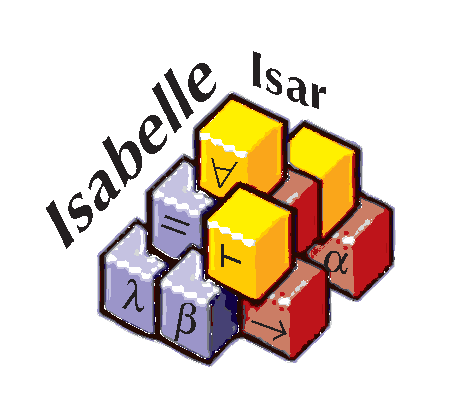
\includegraphics[scale=0.5]{isabelle_isar} \\[4ex] The Isabelle/Isar Reference Manual}
\author{\emph{Markus Wenzel} \\ TU M\"unchen}

\makeindex

\railterm{percent,ppercent,underscore,lbrace,rbrace,llbrace,rrbrace}
\railterm{ident,longident,symident,var,textvar,typefree,typevar,nat,string,verbatim,keyword}

\railalias{ident}{\railtoken{ident}}
\railalias{longident}{\railtoken{longident}}
\railalias{symident}{\railtoken{symident}}
\railalias{var}{\railtoken{var}}
\railalias{textvar}{\railtoken{textvar}}
\railalias{typefree}{\railtoken{typefree}}
\railalias{typevar}{\railtoken{typevar}}
\railalias{nat}{\railtoken{nat}}
\railalias{string}{\railtoken{string}}
\railalias{verbatim}{\railtoken{verbatim}}
\railalias{keyword}{\railtoken{keyword}}

\railalias{name}{\railqtoken{name}}
\railalias{nameref}{\railqtoken{nameref}}
\railalias{text}{\railqtoken{text}}
\railalias{type}{\railqtoken{type}}
\railalias{term}{\railqtoken{term}}
\railalias{prop}{\railqtoken{prop}}
\railalias{atom}{\railqtoken{atom}}

\newcommand{\drv}{\mathrel{\vdash}}
\newcommand{\edrv}{\mathop{\drv}\nolimits}
\newcommand{\Or}{\mathrel{\;|\;}}


\setcounter{secnumdepth}{2} \setcounter{tocdepth}{2}

\pagestyle{headings}
\sloppy
\binperiod     %%%treat . like a binary operator

\renewcommand{\phi}{\varphi}

%\includeonly{generic,refcard}


\begin{document}

\underscoreoff

\maketitle 

\begin{abstract}
  \emph{Intelligible semi-automated reasoning} (\emph{Isar}) is a generic
  approach to readable formal proof documents.  It sets out to bridge the
  semantic gap between any internal notions of proof based on primitive
  inferences and tactics, and an appropriate level of abstraction for
  user-level work.  The Isar formal proof language has been designed to
  satisfy quite contradictory requirements, being both ``declarative'' and
  immediately ``executable'', by virtue of the \emph{Isar/VM} interpreter.
  
  The current version of Isabelle offers Isar as an alternative proof language
  interface layer.  The Isabelle/Isar system provides an interpreter for the
  Isar formal proof language.  The input may consist either of proper document
  constructors, or improper auxiliary commands (for diagnostics, exploration
  etc.).  Proof texts consisting of proper elements only, admit a purely
  static reading, thus being intelligible later without requiring dynamic
  replay that is so typical for traditional proof scripts.  Any of the
  Isabelle/Isar commands may be executed in single-steps, so basically the
  interpreter has a proof text debugger already built-in.
  
  Employing the Isar instantiation of \emph{Proof~General}, a generic Emacs
  interface for interactive proof assistants, we arrive at a reasonable
  environment for \emph{live document editing}.  Thus proof texts may be
  developed incrementally by issuing proof commands, including forward and
  backward tracing of partial documents; intermediate states may be inspected
  by diagnostic commands.
  
  The Isar subsystem is tightly integrated into the Isabelle/Pure meta-logic
  implementation.  Theories, theorems, proof procedures etc.\ may be used
  interchangeably between classic Isabelle proof scripts and Isabelle/Isar
  documents.  Isar is as generic as Isabelle, able to support a wide range of
  object-logics.  Currently, the end-user working environment is most complete
  for Isabelle/HOL.
\end{abstract}

\pagenumbering{roman} \tableofcontents \clearfirst

%FIXME
% - HahnBanach paper
% - Freek Widijk's stuff

%FIXME
\nocite{Rudnicki:1992:MizarOverview}
\nocite{Harrison:1996:MizarHOL}
\nocite{Rudnicki:1992:MizarOverview}
\nocite{Trybulec:1993:MizarFeatures}
\nocite{Syme:1997:DECLARE}
\nocite{Syme:1998:thesis}
\nocite{Syme:1999:TPHOL}
\nocite{Zammit:1999:TPHOL}


\chapter{Introduction}

\section{Quick start}

Isar is already part of Isabelle (as of version Isabelle99, or later).  The
\texttt{isabelle} binary provides option \texttt{-I} to run the Isar
interaction loop at startup, rather than the plain ML top-level.  Thus the
quickest way to do anything with Isabelle/Isar is as follows:
\begin{ttbox}
isabelle -I HOL\medskip
\out{> Welcome to Isabelle/HOL (Isabelle99)}\medskip
theory Foo = Main:
constdefs foo :: nat  "foo == 1";
lemma "0 < foo" by (simp add: foo_def);
end
\end{ttbox}
Note that any Isabelle/Isar command may be retracted by \texttt{undo}.

Plain TTY-based interaction like this used to be quite feasible with
traditional tactic based theorem proving, but developing Isar documents
demands some better user-interface support.  \emph{Proof~General}\index{Proof
  General} of LFCS Edinburgh \cite{proofgeneral} offers a generic Emacs-based
environment for interactive theorem provers that does all the cut-and-paste
and forward-backward walk through the document in a very neat way.  Note that
in Isabelle/Isar, the current position within a partial proof document is more
informative than the actual proof state.  Thus Proof~General provides the
canonical working environment for Isabelle/Isar, both for getting acquainted
(e.g.\ by replaying existing Isar documents) and serious production work.

\medskip

The easiest way to use Proof~General is to make it the default Isabelle user
interface.  Just say something like this in your Isabelle settings file (cf.\ 
\cite{isabelle-sys}):
\begin{ttbox}
ISABELLE_INTERFACE=\$ISABELLE_HOME/contrib/ProofGeneral/isar/interface
PROOFGENERAL_OPTIONS=""
\end{ttbox}
You may have to change \texttt{\$ISABELLE_HOME/contrib/ProofGeneral} to the
actual installation directory of Proof~General.  From now on, the capital
\texttt{Isabelle} executable refers to the \texttt{ProofGeneral/isar}
interface.  Its usage is as follows:
\begin{ttbox}
Usage: interface [OPTIONS] [FILES ...]

  Options are:
    -l NAME      logic image name (default $ISABELLE_LOGIC=HOL)
    -p NAME      Emacs program name (default xemacs)
    -u BOOL      use .emacs file (default true)
    -w BOOL      use window system (default true)

  Starts Proof General for Isabelle/Isar with proof documents FILES
  (default Scratch.thy).

  PROOFGENERAL_OPTIONS=
\end{ttbox}
Apart from the command line, the defaults for these options may be overridden
via the \texttt{PROOFGENERAL_OPTIONS} setting as well.  For example, plain GNU
Emacs may be configured as follows:
\begin{ttbox}
PROOFGENERAL_OPTIONS="-p emacs"
\end{ttbox}

With the proper Isabelle interface setup, Isar documents may now be edited by
visiting appropriate theory files, e.g.\ 
\begin{ttbox}
Isabelle \({\langle}isabellehome{\rangle}\)/src/HOL/Isar_examples/BasicLogic.thy
\end{ttbox}
Users of XEmacs may note the tool bar for navigating forward and backward
through the text.  Consult the Proof~General documentation \cite{proofgeneral}
for further basic commands, such as \texttt{c-c return} or \texttt{c-c u}.

\medskip

Occasionally, a user's \texttt{.emacs} contains material that is incompatible
with the version of (X)Emacs that Proof~General prefers.  Then proper startup
may be still achieved by using the \texttt{-u false} option.\footnote{Also
  note that the Emacs lisp files
  \texttt{\$ISABELLE_HOME/etc/proofgeneral-settings.el} and
  \texttt{\$ISABELLE_HOME_USER/etc/proofgeneral-settings.el} are automatically
  loaded by Proof~General if invoked via the interface wrapper script.}


\section{How to write Isar proofs anyway?}

This is one of the key questions, of course.  Isar offers a rather different
approach to formal proof documents than plain old tactic scripts.  Experienced
users of existing interactive theorem proving systems may have to learn
thinking different in order to make effective use of Isabelle/Isar.  On the
other hand, Isabelle/Isar comes much closer to existing mathematical practice
of formal proof, so users with less experience in old-style tactical proving,
but a good understanding of mathematical proof might cope with Isar even
better.

Unfortunately, there is no tutorial on Isabelle/Isar available yet.  This
document really is a \emph{reference manual}.  Nevertheless, we will give some
discussions of the general principles underlying Isar in
chapter~\ref{ch:basics}, and provide some clues of how these may be put into
practice.  Some more background information on Isar is given in
\cite{Wenzel:1999:TPHOL}.  Furthermore, there are several examples distributed
with Isabelle (see directory \texttt{HOL/Isar_examples}).


%%% Local Variables: 
%%% mode: latex
%%% TeX-master: "isar-ref"
%%% End: 

\chapter{The Basics}

\section{Introduction}

This book is a tutorial on how to use the theorem prover Isabelle/HOL as a
specification and verification system. Isabelle is a generic system for
implementing logical formalisms, and Isabelle/HOL is the specialization
of Isabelle for HOL, which abbreviates Higher-Order Logic. We introduce
HOL step by step following the equation
\[ \mbox{HOL} = \mbox{Functional Programming} + \mbox{Logic}. \]
We do not assume that you are familiar with mathematical logic. 
However, we do assume that
you are used to logical and set theoretic notation, as covered
in a good discrete mathematics course~\cite{Rosen-DMA}, and
that you are familiar with the basic concepts of functional
programming~\cite{Bird-Haskell,Hudak-Haskell,paulson-ml2,Thompson-Haskell}.
Although this tutorial initially concentrates on functional programming, do
not be misled: HOL can express most mathematical concepts, and functional
programming is just one particularly simple and ubiquitous instance.

Isabelle~\cite{paulson-isa-book} is implemented in ML~\cite{SML}.  This has
influenced some of Isabelle/HOL's concrete syntax but is otherwise irrelevant
for us: this tutorial is based on
Isabelle/Isar~\cite{isabelle-isar-ref}, an extension of Isabelle which hides
the implementation language almost completely.  Thus the full name of the
system should be Isabelle/Isar/HOL, but that is a bit of a mouthful.

There are other implementations of HOL, in particular the one by Mike Gordon
\index{Gordon, Mike}%
\emph{et al.}, which is usually referred to as ``the HOL system''
\cite{mgordon-hol}. For us, HOL refers to the logical system, and sometimes
its incarnation Isabelle/HOL\@.

A tutorial is by definition incomplete.  Currently the tutorial only
introduces the rudiments of Isar's proof language. To fully exploit the power
of Isar, in particular the ability to write readable and structured proofs,
you need to consult the Isabelle/Isar Reference
Manual~\cite{isabelle-isar-ref} and Wenzel's PhD thesis~\cite{Wenzel-PhD}
which discusses many proof patterns. If you want to use Isabelle's ML level
directly (for example for writing your own proof procedures) see the Isabelle
Reference Manual~\cite{isabelle-ref}; for details relating to HOL see the
Isabelle/HOL manual~\cite{isabelle-HOL}. All manuals have a comprehensive
index.

\section{Theories}
\label{sec:Basic:Theories}

\index{theories|(}%
Working with Isabelle means creating theories. Roughly speaking, a
\textbf{theory} is a named collection of types, functions, and theorems,
much like a module in a programming language or a specification in a
specification language. In fact, theories in HOL can be either. The general
format of a theory \texttt{T} is
\begin{ttbox}
theory T
imports B\(@1\) \(\ldots\) B\(@n\)
begin
{\rmfamily\textit{declarations, definitions, and proofs}}
end
\end{ttbox}\cmmdx{theory}\cmmdx{imports}
where \texttt{B}$@1$ \dots\ \texttt{B}$@n$ are the names of existing
theories that \texttt{T} is based on and \textit{declarations,
    definitions, and proofs} represents the newly introduced concepts
(types, functions etc.) and proofs about them. The \texttt{B}$@i$ are the
direct \textbf{parent theories}\indexbold{parent theories} of~\texttt{T}\@.
Everything defined in the parent theories (and their parents, recursively) is
automatically visible. To avoid name clashes, identifiers can be
\textbf{qualified}\indexbold{identifiers!qualified}
by theory names as in \texttt{T.f} and~\texttt{B.f}. 
Each theory \texttt{T} must
reside in a \textbf{theory file}\index{theory files} named \texttt{T.thy}.

This tutorial is concerned with introducing you to the different linguistic
constructs that can fill the \textit{declarations, definitions, and
    proofs} above.  A complete grammar of the basic
constructs is found in the Isabelle/Isar Reference
Manual~\cite{isabelle-isar-ref}.

HOL's theory collection is available online at
\begin{center}\small
    \url{http://isabelle.in.tum.de/library/HOL/}
\end{center}
and is recommended browsing. Note that most of the theories 
are based on classical Isabelle without the Isar extension. This means that
they look slightly different than the theories in this tutorial, and that all
proofs are in separate ML files.

\begin{warn}
  HOL contains a theory \thydx{Main}, the union of all the basic
  predefined theories like arithmetic, lists, sets, etc.  
  Unless you know what you are doing, always include \isa{Main}
  as a direct or indirect parent of all your theories.
\end{warn}
There is also a growing Library~\cite{HOL-Library}\index{Library}
of useful theories that are not part of \isa{Main} but can be included
among the parents of a theory and will then be loaded automatically.%
\index{theories|)}


\section{Types, Terms and Formulae}
\label{sec:TypesTermsForms}

Embedded in a theory are the types, terms and formulae of HOL\@. HOL is a typed
logic whose type system resembles that of functional programming languages
like ML or Haskell. Thus there are
\index{types|(}
\begin{description}
\item[base types,] 
in particular \tydx{bool}, the type of truth values,
and \tydx{nat}, the type of natural numbers.
\item[type constructors,]\index{type constructors}
 in particular \tydx{list}, the type of
lists, and \tydx{set}, the type of sets. Type constructors are written
postfix, e.g.\ \isa{(nat)list} is the type of lists whose elements are
natural numbers. Parentheses around single arguments can be dropped (as in
\isa{nat list}), multiple arguments are separated by commas (as in
\isa{(bool,nat)ty}).
\item[function types,]\index{function types}
denoted by \isasymFun\indexbold{$IsaFun@\isasymFun}.
  In HOL \isasymFun\ represents \emph{total} functions only. As is customary,
  \isa{$\tau@1$ \isasymFun~$\tau@2$ \isasymFun~$\tau@3$} means
  \isa{$\tau@1$ \isasymFun~($\tau@2$ \isasymFun~$\tau@3$)}. Isabelle also
  supports the notation \isa{[$\tau@1,\dots,\tau@n$] \isasymFun~$\tau$}
  which abbreviates \isa{$\tau@1$ \isasymFun~$\cdots$ \isasymFun~$\tau@n$
    \isasymFun~$\tau$}.
\item[type variables,]\index{type variables}\index{variables!type}
  denoted by \ttindexboldpos{'a}{$Isatype}, \isa{'b} etc., just like in ML\@. They give rise
  to polymorphic types like \isa{'a \isasymFun~'a}, the type of the identity
  function.
\end{description}
\begin{warn}
  Types are extremely important because they prevent us from writing
  nonsense.  Isabelle insists that all terms and formulae must be well-typed
  and will print an error message if a type mismatch is encountered. To
  reduce the amount of explicit type information that needs to be provided by
  the user, Isabelle infers the type of all variables automatically (this is
  called \bfindex{type inference}) and keeps quiet about it. Occasionally
  this may lead to misunderstandings between you and the system. If anything
  strange happens, we recommend that you set the flag\index{flags}
  \isa{show_types}\index{*show_types (flag)}.  
  Isabelle will then display type information
  that is usually suppressed.  Simply type
\begin{ttbox}
ML "set show_types"
\end{ttbox}

\noindent
This can be reversed by \texttt{ML "reset show_types"}. Various other flags,
which we introduce as we go along, can be set and reset in the same manner.%
\index{flags!setting and resetting}
\end{warn}%
\index{types|)}


\index{terms|(}
\textbf{Terms} are formed as in functional programming by
applying functions to arguments. If \isa{f} is a function of type
\isa{$\tau@1$ \isasymFun~$\tau@2$} and \isa{t} is a term of type
$\tau@1$ then \isa{f~t} is a term of type $\tau@2$. HOL also supports
infix functions like \isa{+} and some basic constructs from functional
programming, such as conditional expressions:
\begin{description}
\item[\isa{if $b$ then $t@1$ else $t@2$}]\index{*if expressions}
Here $b$ is of type \isa{bool} and $t@1$ and $t@2$ are of the same type.
\item[\isa{let $x$ = $t$ in $u$}]\index{*let expressions}
is equivalent to $u$ where all free occurrences of $x$ have been replaced by
$t$. For example,
\isa{let x = 0 in x+x} is equivalent to \isa{0+0}. Multiple bindings are separated
by semicolons: \isa{let $x@1$ = $t@1$;\dots; $x@n$ = $t@n$ in $u$}.
\item[\isa{case $e$ of $c@1$ \isasymFun~$e@1$ |~\dots~| $c@n$ \isasymFun~$e@n$}]
\index{*case expressions}
evaluates to $e@i$ if $e$ is of the form $c@i$.
\end{description}

Terms may also contain
\isasymlambda-abstractions.\index{lambda@$\lambda$ expressions}
For example,
\isa{\isasymlambda{}x.~x+1} is the function that takes an argument \isa{x} and
returns \isa{x+1}. Instead of
\isa{\isasymlambda{}x.\isasymlambda{}y.\isasymlambda{}z.~$t$} we can write
\isa{\isasymlambda{}x~y~z.~$t$}.%
\index{terms|)}

\index{formulae|(}%
\textbf{Formulae} are terms of type \tydx{bool}.
There are the basic constants \cdx{True} and \cdx{False} and
the usual logical connectives (in decreasing order of priority):
\indexboldpos{\protect\isasymnot}{$HOL0not}, \indexboldpos{\protect\isasymand}{$HOL0and},
\indexboldpos{\protect\isasymor}{$HOL0or}, and \indexboldpos{\protect\isasymimp}{$HOL0imp},
all of which (except the unary \isasymnot) associate to the right. In
particular \isa{A \isasymimp~B \isasymimp~C} means \isa{A \isasymimp~(B
  \isasymimp~C)} and is thus logically equivalent to \isa{A \isasymand~B
  \isasymimp~C} (which is \isa{(A \isasymand~B) \isasymimp~C}).

Equality\index{equality} is available in the form of the infix function
\isa{=} of type \isa{'a \isasymFun~'a
  \isasymFun~bool}. Thus \isa{$t@1$ = $t@2$} is a formula provided $t@1$
and $t@2$ are terms of the same type. If $t@1$ and $t@2$ are of type
\isa{bool} then \isa{=} acts as \rmindex{if-and-only-if}.
The formula
\isa{$t@1$~\isasymnoteq~$t@2$} is merely an abbreviation for
\isa{\isasymnot($t@1$ = $t@2$)}.

Quantifiers\index{quantifiers} are written as
\isa{\isasymforall{}x.~$P$} and \isa{\isasymexists{}x.~$P$}. 
There is even
\isa{\isasymuniqex{}x.~$P$}, which
means that there exists exactly one \isa{x} that satisfies \isa{$P$}. 
Nested quantifications can be abbreviated:
\isa{\isasymforall{}x~y~z.~$P$} means
\isa{\isasymforall{}x.\isasymforall{}y.\isasymforall{}z.~$P$}.%
\index{formulae|)}

Despite type inference, it is sometimes necessary to attach explicit
\bfindex{type constraints} to a term.  The syntax is
\isa{$t$::$\tau$} as in \isa{x < (y::nat)}. Note that
\ttindexboldpos{::}{$Isatype} binds weakly and should therefore be enclosed
in parentheses.  For instance,
\isa{x < y::nat} is ill-typed because it is interpreted as
\isa{(x < y)::nat}.  Type constraints may be needed to disambiguate
expressions
involving overloaded functions such as~\isa{+}, 
\isa{*} and~\isa{<}.  Section~\ref{sec:overloading} 
discusses overloading, while Table~\ref{tab:overloading} presents the most
important overloaded function symbols.

In general, HOL's concrete \rmindex{syntax} tries to follow the conventions of
functional programming and mathematics.  Here are the main rules that you
should be familiar with to avoid certain syntactic traps:
\begin{itemize}
\item
Remember that \isa{f t u} means \isa{(f t) u} and not \isa{f(t u)}!
\item
Isabelle allows infix functions like \isa{+}. The prefix form of function
application binds more strongly than anything else and hence \isa{f~x + y}
means \isa{(f~x)~+~y} and not \isa{f(x+y)}.
\item Remember that in HOL if-and-only-if is expressed using equality.  But
  equality has a high priority, as befitting a relation, while if-and-only-if
  typically has the lowest priority.  Thus, \isa{\isasymnot~\isasymnot~P =
    P} means \isa{\isasymnot\isasymnot(P = P)} and not
  \isa{(\isasymnot\isasymnot P) = P}. When using \isa{=} to mean
  logical equivalence, enclose both operands in parentheses, as in \isa{(A
    \isasymand~B) = (B \isasymand~A)}.
\item
Constructs with an opening but without a closing delimiter bind very weakly
and should therefore be enclosed in parentheses if they appear in subterms, as
in \isa{(\isasymlambda{}x.~x) = f}.  This includes 
\isa{if},\index{*if expressions}
\isa{let},\index{*let expressions}
\isa{case},\index{*case expressions}
\isa{\isasymlambda}, and quantifiers.
\item
Never write \isa{\isasymlambda{}x.x} or \isa{\isasymforall{}x.x=x}
because \isa{x.x} is always taken as a single qualified identifier. Write
\isa{\isasymlambda{}x.~x} and \isa{\isasymforall{}x.~x=x} instead.
\item Identifiers\indexbold{identifiers} may contain the characters \isa{_} 
and~\isa{'}, except at the beginning.
\end{itemize}

For the sake of readability, we use the usual mathematical symbols throughout
the tutorial. Their \textsc{ascii}-equivalents are shown in table~\ref{tab:ascii} in
the appendix.

\begin{warn}
A particular
problem for novices can be the priority of operators. If you are unsure, use
additional parentheses. In those cases where Isabelle echoes your
input, you can see which parentheses are dropped --- they were superfluous. If
you are unsure how to interpret Isabelle's output because you don't know
where the (dropped) parentheses go, set the flag\index{flags}
\isa{show_brackets}\index{*show_brackets (flag)}:
\begin{ttbox}
ML "set show_brackets"; \(\dots\); ML "reset show_brackets";
\end{ttbox}
\end{warn}


\section{Variables}
\label{sec:variables}
\index{variables|(}

Isabelle distinguishes free and bound variables, as is customary. Bound
variables are automatically renamed to avoid clashes with free variables. In
addition, Isabelle has a third kind of variable, called a \textbf{schematic
  variable}\index{variables!schematic} or \textbf{unknown}\index{unknowns}, 
which must have a~\isa{?} as its first character.  
Logically, an unknown is a free variable. But it may be
instantiated by another term during the proof process. For example, the
mathematical theorem $x = x$ is represented in Isabelle as \isa{?x = ?x},
which means that Isabelle can instantiate it arbitrarily. This is in contrast
to ordinary variables, which remain fixed. The programming language Prolog
calls unknowns {\em logical\/} variables.

Most of the time you can and should ignore unknowns and work with ordinary
variables. Just don't be surprised that after you have finished the proof of
a theorem, Isabelle will turn your free variables into unknowns.  It
indicates that Isabelle will automatically instantiate those unknowns
suitably when the theorem is used in some other proof.
Note that for readability we often drop the \isa{?}s when displaying a theorem.
\begin{warn}
  For historical reasons, Isabelle accepts \isa{?} as an ASCII representation
  of the \(\exists\) symbol.  However, the \isa{?} character must then be followed
  by a space, as in \isa{?~x. f(x) = 0}.  Otherwise, \isa{?x} is
  interpreted as a schematic variable.  The preferred ASCII representation of
  the \(\exists\) symbol is \isa{EX}\@. 
\end{warn}%
\index{variables|)}

\section{Interaction and Interfaces}

Interaction with Isabelle can either occur at the shell level or through more
advanced interfaces. To keep the tutorial independent of the interface, we
have phrased the description of the interaction in a neutral language. For
example, the phrase ``to abandon a proof'' means to type \isacommand{oops} at the
shell level, which is explained the first time the phrase is used. Other
interfaces perform the same act by cursor movements and/or mouse clicks.
Although shell-based interaction is quite feasible for the kind of proof
scripts currently presented in this tutorial, the recommended interface for
Isabelle/Isar is the Emacs-based \bfindex{Proof
  General}~\cite{proofgeneral,Aspinall:TACAS:2000}.

Some interfaces (including the shell level) offer special fonts with
mathematical symbols. For those that do not, remember that \textsc{ascii}-equivalents
are shown in table~\ref{tab:ascii} in the appendix.

Finally, a word about semicolons.\indexbold{$Isar@\texttt{;}} 
Commands may but need not be terminated by semicolons.
At the shell level it is advisable to use semicolons to enforce that a command
is executed immediately; otherwise Isabelle may wait for the next keyword
before it knows that the command is complete.


\section{Getting Started}

Assuming you have installed Isabelle, you start it by typing \texttt{isabelle
  -I HOL} in a shell window.\footnote{Simply executing \texttt{isabelle -I}
  starts the default logic, which usually is already \texttt{HOL}.  This is
  controlled by the \texttt{ISABELLE_LOGIC} setting, see \emph{The Isabelle
    System Manual} for more details.} This presents you with Isabelle's most
basic \textsc{ascii} interface.  In addition you need to open an editor window to
create theory files.  While you are developing a theory, we recommend that you
type each command into the file first and then enter it into Isabelle by
copy-and-paste, thus ensuring that you have a complete record of your theory.
As mentioned above, Proof General offers a much superior interface.
If you have installed Proof General, you can start it by typing \texttt{Isabelle}.


\chapter{Syntax primitives}

The rather generic framework of Isabelle/Isar syntax emerges from three main
syntactic categories: \emph{commands} of the top-level Isar engine (covering
theory and proof elements), \emph{methods} for general goal refinements
(analogous to traditional ``tactics''), and \emph{attributes} for operations
on facts (within a certain context).  Here we give a reference of basic
syntactic entities underlying Isabelle/Isar syntax in a bottom-up manner.
Concrete theory and proof language elements will be introduced later on.

\medskip

In order to get started with writing well-formed Isabelle/Isar documents, the
most important aspect to be noted is the difference of \emph{inner} versus
\emph{outer} syntax.  Inner syntax is that of Isabelle types and terms of the
logic, while outer syntax is that of Isabelle/Isar theory sources (including
proofs).  As a general rule, inner syntax entities may occur only as
\emph{atomic entities} within outer syntax.  For example, the string
\texttt{"x + y"} and identifier \texttt{z} are legal term specifications
within a theory, while \texttt{x + y} is not.

\begin{warn}
  Old-style Isabelle theories used to fake parts of the inner syntax of types,
  with rather complicated rules when quotes may be omitted.  Despite the minor
  drawback of requiring quotes more often, the syntax of Isabelle/Isar is
  somewhat simpler and more robust in that respect.
\end{warn}

Printed theory documents usually omit quotes to gain readability (this is a
matter of {\LaTeX} macro setup, say via \verb,\isabellestyle,, see also
\cite{isabelle-sys}).  Experienced users of Isabelle/Isar may easily
reconstruct the lost technical information, while mere readers need not care
about quotes at all.

\medskip

Isabelle/Isar input may contain any number of input termination characters
``\texttt{;}'' (semicolon) to separate commands explicitly.  This is
particularly useful in interactive shell sessions to make clear where the
current command is intended to end.  Otherwise, the interpreter loop will
continue to issue a secondary prompt ``\verb,#,'' until an end-of-command is
clearly recognized from the input syntax, e.g.\ encounter of the next command
keyword.

Advanced interfaces such as Proof~General \cite{proofgeneral} do not require
explicit semicolons, the amount of input text is determined automatically by
inspecting the present content of the Emacs text buffer.  In the printed
presentation of Isabelle/Isar documents semicolons are omitted altogether for
readability.

\begin{warn}
  Proof~General requires certain syntax classification tables in order to
  achieve properly synchronized interaction with the Isabelle/Isar process.
  These tables need to be consistent with the Isabelle version and particular
  logic image to be used in a running session (common object-logics may well
  change the outer syntax).  The standard setup should work correctly with any
  of the ``official'' logic images derived from Isabelle/HOL (including HOLCF
  etc.).  Users of alternative logics may need to tell Proof~General
  explicitly, e.g.\ by giving an option \verb,-k ZF, (in conjunction with
  \verb,-l ZF, to specify the default logic image).
\end{warn}

\section{Lexical matters}\label{sec:lex-syntax}

The Isabelle/Isar outer syntax provides token classes as presented below; most
of these coincide with the inner lexical syntax as presented in
\cite{isabelle-ref}.

\indexoutertoken{ident}\indexoutertoken{longident}\indexoutertoken{symident}
\indexoutertoken{nat}\indexoutertoken{var}\indexoutertoken{typefree}
\indexoutertoken{typevar}\indexoutertoken{string}\indexoutertoken{altstring}
\indexoutertoken{verbatim}
\begin{matharray}{rcl}
  ident & = & letter\,quasiletter^* \\
  longident & = & ident (\verb,.,ident)^+ \\
  symident & = & sym^+ ~|~ \verb,\<,ident\verb,>, \\
  nat & = & digit^+ \\
  var & = & ident ~|~ \verb,?,ident ~|~ \verb,?,ident\verb,.,nat \\
  typefree & = & \verb,',ident \\
  typevar & = & typefree ~|~ \verb,?,typefree ~|~ \verb,?,typefree\verb,.,nat \\
  string & = & \verb,", ~\dots~ \verb,", \\
  altstring & = & \backquote ~\dots~ \backquote \\
  verbatim & = & \verb,{*, ~\dots~ \verb,*}, \\[1ex]

  letter & = & latin ~|~ \verb,\<,latin\verb,>, ~|~ \verb,\<,latin\,latin\verb,>, ~|~ greek ~|~ \\
         &   & \verb,\<^isub>, ~|~ \verb,\<^isup>, \\
  quasiletter & = & letter ~|~ digit ~|~ \verb,_, ~|~ \verb,', \\
  latin & = & \verb,a, ~|~ \dots ~|~ \verb,z, ~|~ \verb,A, ~|~ \dots ~|~ \verb,Z, \\
  digit & = & \verb,0, ~|~ \dots ~|~ \verb,9, \\
  sym & = & \verb,!, ~|~ \verb,#, ~|~ \verb,$, ~|~ \verb,%, ~|~ \verb,&, ~|~  %$
   \verb,*, ~|~ \verb,+, ~|~ \verb,-, ~|~ \verb,/, ~|~ \\
  & & \verb,<, ~|~ \verb,=, ~|~ \verb,>, ~|~ \verb,?, ~|~ \texttt{\at} ~|~
  \verb,^, ~|~ \verb,_, ~|~ \verb,|, ~|~ \verb,~, \\
greek & = & \verb,\<alpha>, ~|~ \verb,\<beta>, ~|~ \verb,\<gamma>, ~|~ \verb,\<delta>, ~| \\
      &   & \verb,\<epsilon>, ~|~ \verb,\<zeta>, ~|~ \verb,\<eta>, ~|~ \verb,\<theta>, ~| \\
      &   & \verb,\<iota>, ~|~ \verb,\<kappa>, ~|~ \verb,\<mu>, ~|~ \verb,\<nu>, ~| \\
      &   & \verb,\<xi>, ~|~ \verb,\<pi>, ~|~ \verb,\<rho>, ~|~ \verb,\<sigma>, ~| \\
      &   & \verb,\<tau>, ~|~ \verb,\<upsilon>, ~|~ \verb,\<phi>, ~|~ \verb,\<psi>, ~| \\
      &   & \verb,\<omega>, ~|~ \verb,\<Gamma>, ~|~ \verb,\<Delta>, ~|~ \verb,\<Theta>, ~| \\
      &   & \verb,\<Lambda>, ~|~ \verb,\<Xi>, ~|~ \verb,\<Pi>, ~|~ \verb,\<Sigma>, ~| \\
      &   & \verb,\<Upsilon>, ~|~ \verb,\<Phi>, ~|~ \verb,\<Psi>, ~|~ \verb,\<Omega>, \\
\end{matharray}

The syntax of $string$ admits any characters, including newlines; ``\verb|"|''
(double-quote) and ``\verb|\|'' (backslash) need to be escaped by a backslash.
Alternative strings according to $altstring$ are analogous, using single
back-quotes instead.  The body of $verbatim$ may consist of any text not
containing ``\verb|*}|''; this allows convenient inclusion of quotes without
further escapes.  The greek letters do \emph{not} include \verb,\<lambda>,,
which is already used differently in the meta-logic.

Common mathematical symbols such as $\forall$ are represented in Isabelle as
\verb,\<forall>,.  There are infinitely many legal symbols like this, although
proper presentation is left to front-end tools such as {\LaTeX} or
Proof~General with the X-Symbol package.  A list of standard Isabelle symbols
that work well with these tools is given in \cite[appendix~A]{isabelle-sys}.

Comments take the form \texttt{(*~\dots~*)} and may be nested, although
user-interface tools may prevent this.  Note that \texttt{(*~\dots~*)}
indicate source comments only, which are stripped after lexical analysis of
the input.  The Isar document syntax also provides formal comments that are
considered as part of the text (see \S\ref{sec:comments}).

\begin{warn}
  Proof~General does not handle nested comments properly; it is also unable to
  keep \verb,(*,\,/\,\verb,{*, and \verb,*),\,/\,\verb,*}, apart, despite
  their rather different meaning.  These are inherent problems of Emacs
  legacy.  Users should not be overly aggressive about nesting or alternating
  these delimiters.
\end{warn}


\section{Common syntax entities}

Subsequently, we introduce several basic syntactic entities, such as names,
terms, and theorem specifications, which have been factored out of the actual
Isar language elements to be described later.

Note that some of the basic syntactic entities introduced below (e.g.\
\railqtok{name}) act much like tokens rather than plain nonterminals (e.g.\
\railnonterm{sort}), especially for the sake of error messages.  E.g.\ syntax
elements like $\CONSTS$ referring to \railqtok{name} or \railqtok{type} would
really report a missing name or type rather than any of the constituent
primitive tokens such as \railtok{ident} or \railtok{string}.


\subsection{Names}

Entity \railqtok{name} usually refers to any name of types, constants,
theorems etc.\ that are to be \emph{declared} or \emph{defined} (so qualified
identifiers are excluded here).  Quoted strings provide an escape for
non-identifier names or those ruled out by outer syntax keywords (e.g.\
\verb|"let"|).  Already existing objects are usually referenced by
\railqtok{nameref}.

\indexoutertoken{name}\indexoutertoken{parname}\indexoutertoken{nameref}
\indexoutertoken{int}
\begin{rail}
  name: ident | symident | string | nat
  ;
  parname: '(' name ')'
  ;
  nameref: name | longident
  ;
  int: nat | '-' nat
  ;
\end{rail}


\subsection{Comments}\label{sec:comments}

Large chunks of plain \railqtok{text} are usually given \railtok{verbatim},
i.e.\ enclosed in \verb|{*|~\dots~\verb|*}|.  For convenience, any of the
smaller text units conforming to \railqtok{nameref} are admitted as well.  A
marginal \railnonterm{comment} is of the form \texttt{--} \railqtok{text}.
Any number of these may occur within Isabelle/Isar commands.

\indexoutertoken{text}\indexouternonterm{comment}
\begin{rail}
  text: verbatim | nameref
  ;
  comment: '--' text
  ;
\end{rail}


\subsection{Type classes, sorts and arities}

Classes are specified by plain names.  Sorts have a very simple inner syntax,
which is either a single class name $c$ or a list $\{c@1, \dots, c@n\}$
referring to the intersection of these classes.  The syntax of type arities is
given directly at the outer level.

\railalias{subseteq}{\isasymsubseteq}
\railterm{subseteq}

\indexouternonterm{sort}\indexouternonterm{arity}
\indexouternonterm{classdecl}
\begin{rail}
  classdecl: name (('<' | subseteq) (nameref + ','))?
  ;
  sort: nameref
  ;
  arity: ('(' (sort + ',') ')')? sort
  ;
\end{rail}


\subsection{Types and terms}\label{sec:types-terms}

The actual inner Isabelle syntax, that of types and terms of the logic, is far
too sophisticated in order to be modelled explicitly at the outer theory
level.  Basically, any such entity has to be quoted to turn it into a single
token (the parsing and type-checking is performed internally later).  For
convenience, a slightly more liberal convention is adopted: quotes may be
omitted for any type or term that is already atomic at the outer level.  For
example, one may just write \texttt{x} instead of \texttt{"x"}.  Note that
symbolic identifiers (e.g.\ \texttt{++} or $\forall$) are available as well,
provided these have not been superseded by commands or other keywords already
(e.g.\ \texttt{=} or \texttt{+}).

\indexoutertoken{type}\indexoutertoken{term}\indexoutertoken{prop}
\begin{rail}
  type: nameref | typefree | typevar
  ;
  term: nameref | var
  ;
  prop: term
  ;
\end{rail}

Positional instantiations are indicated by giving a sequence of terms, or the
placeholder ``$\_$'' (underscore), which means to skip a position.

\indexoutertoken{inst}\indexoutertoken{insts}
\begin{rail}
  inst: underscore | term
  ;
  insts: (inst *)
  ;
\end{rail}

Type declarations and definitions usually refer to \railnonterm{typespec} on
the left-hand side.  This models basic type constructor application at the
outer syntax level.  Note that only plain postfix notation is available here,
but no infixes.

\indexouternonterm{typespec}
\begin{rail}
  typespec: (() | typefree | '(' ( typefree + ',' ) ')') name
  ;
\end{rail}


\subsection{Mixfix annotations}

Mixfix annotations specify concrete \emph{inner} syntax of Isabelle types and
terms.  Some commands such as $\TYPES$ (see \S\ref{sec:types-pure}) admit
infixes only, while $\CONSTS$ (see \S\ref{sec:consts}) and
$\isarkeyword{syntax}$ (see \S\ref{sec:syn-trans}) support the full range of
general mixfixes and binders.

\indexouternonterm{infix}\indexouternonterm{mixfix}\indexouternonterm{structmixfix}
\begin{rail}
  infix: '(' ('infix' | 'infixl' | 'infixr') string? nat ')'
  ;
  mixfix: infix | '(' string prios? nat? ')' | '(' 'binder' string prios? nat ')'
  ;
  structmixfix: mixfix | '(' 'structure' ')'
  ;

  prios: '[' (nat + ',') ']'
  ;
\end{rail}

Here the \railtok{string} specifications refer to the actual mixfix template
(see also \cite{isabelle-ref}), which may include literal text, spacing,
blocks, and arguments (denoted by ``$_$''); the special symbol \verb,\<index>,
(printed as ``\i'') represents an index argument that specifies an implicit
structure reference (see also \S\ref{sec:locale}).  Infix and binder
declarations provide common abbreviations for particular mixfix declarations.
So in practice, mixfix templates mostly degenerate to literal text for
concrete syntax, such as ``\verb,++,'' for an infix symbol, or ``\verb,++,\i''
for an infix of an implicit structure.



\subsection{Proof methods}\label{sec:syn-meth}

Proof methods are either basic ones, or expressions composed of
methods via ``\texttt{,}'' (sequential composition), ``\texttt{|}''
(alternative choices), ``\texttt{?}'' (try), ``\texttt{+}'' (repeat at
least once), ``\texttt{[$n$]}'' (restriction to first $n$ sub-goals,
default $n = 1$).  In practice, proof methods are usually just a comma
separated list of \railqtok{nameref}~\railnonterm{args}
specifications.  Note that parentheses may be dropped for single
method specifications (with no arguments).

\indexouternonterm{method}
\begin{rail}
  method: (nameref | '(' methods ')') (() | '?' | '+' | '[' nat? ']')
  ;
  methods: (nameref args | method) + (',' | '|')
  ;
\end{rail}

Proper Isar proof methods do \emph{not} admit arbitrary goal
addressing, but refer either to the first sub-goal or all sub-goals
uniformly.  The goal restriction operator ``\texttt{[$n$]}'' evaluates
a method expression within a sandbox consisting of the first $n$
sub-goals (which need to exist).  For example,
$simp_all\mbox{\tt[}3\mbox{\tt]}$ simplifies the first three
sub-goals, while $(rule~foo, simp_all)\mbox{\tt[]}$ simplifies all new
goals that emerge from applying rule $foo$ to the originally first
one.

Improper methods, notably tactic emulations, offer a separate
low-level goal addressing scheme as explicit argument to the
individual tactic being involved.  Here $[!]$ refers to all goals, and
$[n-]$ to all goals starting from $n$,

\indexouternonterm{goalspec}
\begin{rail}
  goalspec: '[' (nat '-' nat | nat '-' | nat | '!' ) ']'
  ;
\end{rail}


\subsection{Attributes and theorems}\label{sec:syn-att}

Attributes (and proof methods, see \S\ref{sec:syn-meth}) have their own
``semi-inner'' syntax, in the sense that input conforming to
\railnonterm{args} below is parsed by the attribute a second time.  The
attribute argument specifications may be any sequence of atomic entities
(identifiers, strings etc.), or properly bracketed argument lists.  Below
\railqtok{atom} refers to any atomic entity, including any \railtok{keyword}
conforming to \railtok{symident}.

\indexoutertoken{atom}\indexouternonterm{args}\indexouternonterm{attributes}
\begin{rail}
  atom: nameref | typefree | typevar | var | nat | keyword
  ;
  arg: atom | '(' args ')' | '[' args ']'
  ;
  args: arg *
  ;
  attributes: '[' (nameref args * ',') ']'
  ;
\end{rail}

Theorem specifications come in several flavors: \railnonterm{axmdecl} and
\railnonterm{thmdecl} usually refer to axioms, assumptions or results of goal
statements, while \railnonterm{thmdef} collects lists of existing theorems.
Existing theorems are given by \railnonterm{thmref} and \railnonterm{thmrefs},
the former requires an actual singleton result.  There are three forms of
theorem references: (1) named facts $a$, (2) selections from named facts $a(i,
j - k)$, or (3) literal fact propositions using $altstring$ syntax
$\backquote\phi\backquote$, (see also method $fact$ in
\S\ref{sec:pure-meth-att}).

Any kind of theorem specification may include lists of attributes both on the
left and right hand sides; attributes are applied to any immediately preceding
fact.  If names are omitted, the theorems are not stored within the theorem
database of the theory or proof context, but any given attributes are applied
nonetheless.

\indexouternonterm{axmdecl}\indexouternonterm{thmdecl}
\indexouternonterm{thmdef}\indexouternonterm{thmref}
\indexouternonterm{thmrefs}\indexouternonterm{selection}
\begin{rail}
  axmdecl: name attributes? ':'
  ;
  thmdecl: thmbind ':'
  ;
  thmdef: thmbind '='
  ;
  thmref: (nameref selection? | altstring) attributes?
  ;
  thmrefs: thmref +
  ;

  thmbind: name attributes | name | attributes
  ;
  selection: '(' ((nat | nat '-' nat?) + ',') ')'
  ;
\end{rail}


\subsection{Term patterns and declarations}\label{sec:term-decls}

Wherever explicit propositions (or term fragments) occur in a proof text,
casual binding of schematic term variables may be given specified via patterns
of the form ``$\ISS{p@1\;\dots}{p@n}$''.  There are separate versions
available for \railqtok{term}s and \railqtok{prop}s.  The latter provides a
$\CONCLNAME$ part with patterns referring the (atomic) conclusion of a rule.

\indexouternonterm{termpat}\indexouternonterm{proppat}
\begin{rail}
  termpat: '(' ('is' term +) ')'
  ;
  proppat: '(' ('is' prop +) ')'
  ;
\end{rail}

Declarations of local variables $x :: \tau$ and logical propositions $a :
\phi$ represent different views on the same principle of introducing a local
scope.  In practice, one may usually omit the typing of $vars$ (due to
type-inference), and the naming of propositions (due to implicit references of
current facts).  In any case, Isar proof elements usually admit to introduce
multiple such items simultaneously.

\indexouternonterm{vars}\indexouternonterm{props}
\begin{rail}
  vars: (name+) ('::' type)?
  ;
  props: thmdecl? (prop proppat? +)
  ;
\end{rail}

The treatment of multiple declarations corresponds to the complementary focus
of $vars$ versus $props$: in ``$x@1~\dots~x@n :: \tau$'' the typing refers to
all variables, while in $a\colon \phi@1~\dots~\phi@n$ the naming refers to all
propositions collectively.  Isar language elements that refer to $vars$ or
$props$ typically admit separate typings or namings via another level of
iteration, with explicit $\AND$ separators; e.g.\ see $\FIXNAME$ and
$\ASSUMENAME$ in \S\ref{sec:proof-context}.


\subsection{Antiquotations}\label{sec:antiq}

\begin{matharray}{rcl}
  theory & : & \isarantiq \\
  thm & : & \isarantiq \\
  prop & : & \isarantiq \\
  term & : & \isarantiq \\
  const & : & \isarantiq \\
  abbrev & : & \isarantiq \\
  typeof & : & \isarantiq \\
  typ & : & \isarantiq \\
  thm_style & : & \isarantiq \\
  term_style & : & \isarantiq \\
  text & : & \isarantiq \\
  goals & : & \isarantiq \\
  subgoals & : & \isarantiq \\
  prf & : & \isarantiq \\
  full_prf & : & \isarantiq \\
  ML & : & \isarantiq \\
  ML_type & : & \isarantiq \\
  ML_struct & : & \isarantiq \\
\end{matharray}

The text body of formal comments (see also \S\ref{sec:comments}) may contain
antiquotations of logical entities, such as theorems, terms and types, which
are to be presented in the final output produced by the Isabelle document
preparation system (see also \S\ref{sec:document-prep}).

Thus embedding of
``\texttt{{\at}{\ttlbrace}term~[show_types]~"f(x)~=~a~+~x"{\ttrbrace}}''
within a text block would cause
\isa{(f{\isasymColon}'a~{\isasymRightarrow}~'a)~(x{\isasymColon}'a)~=~(a{\isasymColon}'a)~+~x}
to appear in the final {\LaTeX} document.  Also note that theorem
antiquotations may involve attributes as well.  For example,
\texttt{{\at}{\ttlbrace}thm~sym~[no_vars]{\ttrbrace}} would print the
statement where all schematic variables have been replaced by fixed ones,
which are easier to read.

\indexisarant{theory}\indexisarant{thm}\indexisarant{prop}\indexisarant{term}\indexisarant{const}
\indexisarant{abbrev}\indexisarant{typeof}\indexisarant{typ}\indexisarant{thm-style}
\indexisarant{term-style}\indexisarant{text}\indexisarant{goals}
\indexisarant{subgoals}\indexisarant{prf}\indexisarant{full-prf}\indexisarant{ML}
\indexisarant{ML-type}\indexisarant{ML-struct}

\begin{rail}
  atsign lbrace antiquotation rbrace
  ;

  antiquotation:
    'theory' options name |
    'thm' options thmrefs |
    'prop' options prop |
    'term' options term |
    'const' options term |
    'abbrev' options term |
    'typeof' options term |
    'typ' options type |
    'thm\_style' options name thmref |
    'term\_style' options name term |
    'text' options name |
    'goals' options |
    'subgoals' options |
    'prf' options thmrefs |
    'full\_prf' options thmrefs |
    'ML' options name |
    'ML\_type' options name |
    'ML\_struct' options name
  ;
  options: '[' (option * ',') ']'
  ;
  option: name | name '=' name
  ;
\end{rail}

Note that the syntax of antiquotations may \emph{not} include source comments
\texttt{(*~\dots~*)} or verbatim text \verb|{*|~\dots~\verb|*}|.

\begin{descr}
  
\item [$\at\{theory~A\}$] prints the name $A$, which is guaranteed to
  refer to a valid ancestor theory in the current context.

\item [$\at\{thm~\vec a\}$] prints theorems $\vec a$. Note that attribute
  specifications may be included as well (see also \S\ref{sec:syn-att}); the
  $no_vars$ operation (see \S\ref{sec:misc-meth-att}) would be particularly
  useful to suppress printing of schematic variables.

\item [$\at\{prop~\phi\}$] prints a well-typed proposition $\phi$.

\item [$\at\{term~t\}$] prints a well-typed term $t$.

\item [$\at\{const~c\}$] prints a well-defined constant $c$.
  
\item [$\at\{abbrev~c\,\vec x\}$] prints a constant abbreviation
  $c\,\vec x \equiv rhs$ as defined in the current context.

\item [$\at\{typeof~t\}$] prints the type of a well-typed term $t$.

\item [$\at\{typ~\tau\}$] prints a well-formed type $\tau$.
  
\item [$\at\{thm_style~s~a\}$] prints theorem $a$, previously applying a style
  $s$ to it (see below).
  
\item [$\at\{term_style~s~t\}$] prints a well-typed term $t$ after applying a
  style $s$ to it (see below).

\item [$\at\{text~s\}$] prints uninterpreted source text $s$.  This is
  particularly useful to print portions of text according to the Isabelle
  {\LaTeX} output style, without demanding well-formedness (e.g.\ small pieces
  of terms that should not be parsed or type-checked yet).

\item [$\at\{goals\}$] prints the current \emph{dynamic} goal state.  This is
  mainly for support of tactic-emulation scripts within Isar --- presentation
  of goal states does not conform to actual human-readable proof documents.
  Please do not include goal states into document output unless you really
  know what you are doing!
  
\item [$\at\{subgoals\}$] is similar to $goals$, but does not print the main
  goal.
  
\item [$\at\{prf~\vec a\}$] prints the (compact) proof terms corresponding to
  the theorems $\vec a$. Note that this requires proof terms to be switched on
  for the current object logic (see the ``Proof terms'' section of the
  Isabelle reference manual for information on how to do this).
  
\item [$\at\{full_prf~\vec a\}$] is like $\at\{prf~\vec a\}$, but displays the
  full proof terms, i.e.\ also displays information omitted in the compact
  proof term, which is denoted by ``$_$'' placeholders there.
  
\item [$\at\{ML~s\}$, $\at\{ML_type~s\}$, and $\at\{ML_struct~s\}$] check text
  $s$ as ML value, type, and structure, respectively.  If successful, the
  source is displayed verbatim.

\end{descr}

\medskip

The following standard styles for use with $thm_style$ and $term_style$ are
available:

\begin{descr}
  
\item [$lhs$] extracts the first argument of any application form with at
  least two arguments -- typically meta-level or object-level equality, or any
  other binary relation.
  
\item [$rhs$] is like $lhs$, but extracts the second argument.
  
\item [$concl$] extracts the conclusion $C$ from a nested meta-level
  implication $A@1 \Imp \cdots A@n \Imp C$.
  
\item [$prem1$, \dots, $prem9$] extract premise number $1$, \dots, $9$,
  respectively, from a nested meta-level implication $A@1 \Imp \cdots A@n \Imp
  C$.

\end{descr}

\medskip

The following options are available to tune the output.  Note that most of
these coincide with ML flags of the same names (see also \cite{isabelle-ref}).
\begin{descr}
\item[$show_types = bool$ and $show_sorts = bool$] control printing of
  explicit type and sort constraints.
\item[$show_structs = bool$] controls printing of implicit structures.
\item[$long_names = bool$] forces names of types and constants etc.\ to be
  printed in their fully qualified internal form.
\item[$short_names = bool$] forces names of types and constants etc.\ to be
  printed unqualified.  Note that internalizing the output again in the
  current context may well yield a different result.
\item[$unique_names = bool$] determines whether the printed version of
  qualified names should be made sufficiently long to avoid overlap with names
  declared further back.  Set to $false$ for more concise output.
\item[$eta_contract = bool$] prints terms in $\eta$-contracted form.
\item[$display = bool$] indicates if the text is to be output as multi-line
  ``display material'', rather than a small piece of text without line breaks
  (which is the default).
\item[$breaks = bool$] controls line breaks in non-display material.
\item[$quotes = bool$] indicates if the output should be enclosed in double
  quotes.
\item[$mode = name$] adds $name$ to the print mode to be used for presentation
  (see also \cite{isabelle-ref}).  Note that the standard setup for {\LaTeX}
  output is already present by default, including the modes ``$latex$'',
  ``$xsymbols$'', ``$symbols$''.
\item[$margin = nat$ and $indent = nat$] change the margin or indentation for
  pretty printing of display material.
\item[$source = bool$] prints the source text of the antiquotation arguments,
  rather than the actual value.  Note that this does not affect
  well-formedness checks of $thm$, $term$, etc. (only the $text$ antiquotation
  admits arbitrary output).
\item[$goals_limit = nat$] determines the maximum number of goals to be
  printed.
\item[$locale = name$] specifies an alternative context used for evaluating
  and printing the subsequent argument.
\end{descr}

For boolean flags, ``$name = true$'' may be abbreviated as ``$name$''.  All of
the above flags are disabled by default, unless changed from ML.

\medskip Note that antiquotations do not only spare the author from tedious
typing of logical entities, but also achieve some degree of
consistency-checking of informal explanations with formal developments:
well-formedness of terms and types with respect to the current theory or proof
context is ensured here.


\subsection{Tagged commands}\label{sec:tags}

Each Isabelle/Isar command may be decorated by presentation tags:

\indexouternonterm{tags}
\begin{rail}
  tags: ( tag * )
  ;
  tag: '\%' (ident | string)
\end{rail}

The tags $theory$, $proof$, $ML$ are already pre-declared for certain classes
of commands:

\medskip

\begin{tabular}{ll}
  $theory$ & theory begin and end \\
  $proof$ & all proof commands \\
  $ML$ & all commands involving ML code \\
\end{tabular}

\medskip The Isabelle document preparation system (see also
\cite{isabelle-sys}) allows tagged command regions to be presented
specifically, e.g.\ to fold proof texts, or drop parts of the text completely.

For example ``$\BYNAME~\%invisible~(auto)$'' would cause that piece of proof
to be treated as $invisible$ instead of $proof$ (the default), which may be
either show or hidden depending on the document setup.  In contrast,
``$\BYNAME~\%visible~(auto)$'' would force this text to be shown invariably.

Explicit tag specifications within a proof apply to all subsequent commands of
the same level of nesting.  For example,
``$\PROOFNAME~\%visible~\dots\QEDNAME$'' would force the whole sub-proof to be
typeset as $visible$ (unless some of its parts are tagged differently).

%%% Local Variables:
%%% mode: latex
%%% TeX-master: "isar-ref"
%%% End:

%
\begin{isabellebody}%
\def\isabellecontext{pure}%
%
\isadelimtheory
\isanewline
\isanewline
%
\endisadelimtheory
%
\isatagtheory
\isacommand{theory}\isamarkupfalse%
\ pure\isanewline
\isakeyword{imports}\ Pure\isanewline
\isakeyword{begin}%
\endisatagtheory
{\isafoldtheory}%
%
\isadelimtheory
%
\endisadelimtheory
%
\isamarkupchapter{Basic language elements \label{ch:pure-syntax}%
}
\isamarkuptrue%
%
\isamarkupsection{Other commands%
}
\isamarkuptrue%
%
\isamarkupsubsection{Diagnostics%
}
\isamarkuptrue%
%
\begin{isamarkuptext}%
\begin{matharray}{rcl}
    \indexdef{}{command}{pr}\hypertarget{command.pr}{\hyperlink{command.pr}{\mbox{\isa{\isacommand{pr}}}}}\isa{{\isachardoublequote}\isactrlsup {\isacharasterisk}{\isachardoublequote}} & : & \isarkeep{\cdot} \\
    \indexdef{}{command}{thm}\hypertarget{command.thm}{\hyperlink{command.thm}{\mbox{\isa{\isacommand{thm}}}}}\isa{{\isachardoublequote}\isactrlsup {\isacharasterisk}{\isachardoublequote}} & : & \isarkeep{theory~|~proof} \\
    \indexdef{}{command}{term}\hypertarget{command.term}{\hyperlink{command.term}{\mbox{\isa{\isacommand{term}}}}}\isa{{\isachardoublequote}\isactrlsup {\isacharasterisk}{\isachardoublequote}} & : & \isarkeep{theory~|~proof} \\
    \indexdef{}{command}{prop}\hypertarget{command.prop}{\hyperlink{command.prop}{\mbox{\isa{\isacommand{prop}}}}}\isa{{\isachardoublequote}\isactrlsup {\isacharasterisk}{\isachardoublequote}} & : & \isarkeep{theory~|~proof} \\
    \indexdef{}{command}{typ}\hypertarget{command.typ}{\hyperlink{command.typ}{\mbox{\isa{\isacommand{typ}}}}}\isa{{\isachardoublequote}\isactrlsup {\isacharasterisk}{\isachardoublequote}} & : & \isarkeep{theory~|~proof} \\
    \indexdef{}{command}{prf}\hypertarget{command.prf}{\hyperlink{command.prf}{\mbox{\isa{\isacommand{prf}}}}}\isa{{\isachardoublequote}\isactrlsup {\isacharasterisk}{\isachardoublequote}} & : & \isarkeep{theory~|~proof} \\
    \indexdef{}{command}{full\_prf}\hypertarget{command.full-prf}{\hyperlink{command.full-prf}{\mbox{\isa{\isacommand{full{\isacharunderscore}prf}}}}}\isa{{\isachardoublequote}\isactrlsup {\isacharasterisk}{\isachardoublequote}} & : & \isarkeep{theory~|~proof} \\
  \end{matharray}

  These diagnostic commands assist interactive development.  Note that
  \hyperlink{command.undo}{\mbox{\isa{\isacommand{undo}}}} does not apply here, the theory or proof
  configuration is not changed.

  \begin{rail}
    'pr' modes? nat? (',' nat)?
    ;
    'thm' modes? thmrefs
    ;
    'term' modes? term
    ;
    'prop' modes? prop
    ;
    'typ' modes? type
    ;
    'prf' modes? thmrefs?
    ;
    'full\_prf' modes? thmrefs?
    ;

    modes: '(' (name + ) ')'
    ;
  \end{rail}

  \begin{descr}

  \item [\hyperlink{command.pr}{\mbox{\isa{\isacommand{pr}}}}~\isa{{\isachardoublequote}goals{\isacharcomma}\ prems{\isachardoublequote}}] prints the current
  proof state (if present), including the proof context, current facts
  and goals.  The optional limit arguments affect the number of goals
  and premises to be displayed, which is initially 10 for both.
  Omitting limit values leaves the current setting unchanged.

  \item [\hyperlink{command.thm}{\mbox{\isa{\isacommand{thm}}}}~\isa{{\isachardoublequote}a\isactrlsub {\isadigit{1}}\ {\isasymdots}\ a\isactrlsub n{\isachardoublequote}}] retrieves
  theorems from the current theory or proof context.  Note that any
  attributes included in the theorem specifications are applied to a
  temporary context derived from the current theory or proof; the
  result is discarded, i.e.\ attributes involved in \isa{{\isachardoublequote}a\isactrlsub {\isadigit{1}}{\isacharcomma}\ {\isasymdots}{\isacharcomma}\ a\isactrlsub n{\isachardoublequote}} do not have any permanent effect.

  \item [\hyperlink{command.term}{\mbox{\isa{\isacommand{term}}}}~\isa{t} and \hyperlink{command.prop}{\mbox{\isa{\isacommand{prop}}}}~\isa{{\isasymphi}}]
  read, type-check and print terms or propositions according to the
  current theory or proof context; the inferred type of \isa{t} is
  output as well.  Note that these commands are also useful in
  inspecting the current environment of term abbreviations.

  \item [\hyperlink{command.typ}{\mbox{\isa{\isacommand{typ}}}}~\isa{{\isasymtau}}] reads and prints types of the
  meta-logic according to the current theory or proof context.

  \item [\hyperlink{command.prf}{\mbox{\isa{\isacommand{prf}}}}] displays the (compact) proof term of the
  current proof state (if present), or of the given theorems. Note
  that this requires proof terms to be switched on for the current
  object logic (see the ``Proof terms'' section of the Isabelle
  reference manual for information on how to do this).

  \item [\hyperlink{command.full-prf}{\mbox{\isa{\isacommand{full{\isacharunderscore}prf}}}}] is like \hyperlink{command.prf}{\mbox{\isa{\isacommand{prf}}}}, but displays
  the full proof term, i.e.\ also displays information omitted in the
  compact proof term, which is denoted by ``\isa{{\isacharunderscore}}'' placeholders
  there.

  \end{descr}

  All of the diagnostic commands above admit a list of \isa{modes}
  to be specified, which is appended to the current print mode (see
  also \cite{isabelle-ref}).  Thus the output behavior may be modified
  according particular print mode features.  For example, \hyperlink{command.pr}{\mbox{\isa{\isacommand{pr}}}}~\isa{{\isachardoublequote}{\isacharparenleft}latex\ xsymbols\ symbols{\isacharparenright}{\isachardoublequote}} would print the current
  proof state with mathematical symbols and special characters
  represented in {\LaTeX} source, according to the Isabelle style
  \cite{isabelle-sys}.

  Note that antiquotations (cf.\ \secref{sec:antiq}) provide a more
  systematic way to include formal items into the printed text
  document.%
\end{isamarkuptext}%
\isamarkuptrue%
%
\isamarkupsubsection{Inspecting the context%
}
\isamarkuptrue%
%
\begin{isamarkuptext}%
\begin{matharray}{rcl}
    \indexdef{}{command}{print\_commands}\hypertarget{command.print-commands}{\hyperlink{command.print-commands}{\mbox{\isa{\isacommand{print{\isacharunderscore}commands}}}}}\isa{{\isachardoublequote}\isactrlsup {\isacharasterisk}{\isachardoublequote}} & : & \isarkeep{\cdot} \\
    \indexdef{}{command}{print\_theory}\hypertarget{command.print-theory}{\hyperlink{command.print-theory}{\mbox{\isa{\isacommand{print{\isacharunderscore}theory}}}}}\isa{{\isachardoublequote}\isactrlsup {\isacharasterisk}{\isachardoublequote}} & : & \isarkeep{theory~|~proof} \\
    \indexdef{}{command}{print\_syntax}\hypertarget{command.print-syntax}{\hyperlink{command.print-syntax}{\mbox{\isa{\isacommand{print{\isacharunderscore}syntax}}}}}\isa{{\isachardoublequote}\isactrlsup {\isacharasterisk}{\isachardoublequote}} & : & \isarkeep{theory~|~proof} \\
    \indexdef{}{command}{print\_methods}\hypertarget{command.print-methods}{\hyperlink{command.print-methods}{\mbox{\isa{\isacommand{print{\isacharunderscore}methods}}}}}\isa{{\isachardoublequote}\isactrlsup {\isacharasterisk}{\isachardoublequote}} & : & \isarkeep{theory~|~proof} \\
    \indexdef{}{command}{print\_attributes}\hypertarget{command.print-attributes}{\hyperlink{command.print-attributes}{\mbox{\isa{\isacommand{print{\isacharunderscore}attributes}}}}}\isa{{\isachardoublequote}\isactrlsup {\isacharasterisk}{\isachardoublequote}} & : & \isarkeep{theory~|~proof} \\
    \indexdef{}{command}{print\_theorems}\hypertarget{command.print-theorems}{\hyperlink{command.print-theorems}{\mbox{\isa{\isacommand{print{\isacharunderscore}theorems}}}}}\isa{{\isachardoublequote}\isactrlsup {\isacharasterisk}{\isachardoublequote}} & : & \isarkeep{theory~|~proof} \\
    \indexdef{}{command}{find\_theorems}\hypertarget{command.find-theorems}{\hyperlink{command.find-theorems}{\mbox{\isa{\isacommand{find{\isacharunderscore}theorems}}}}}\isa{{\isachardoublequote}\isactrlsup {\isacharasterisk}{\isachardoublequote}} & : & \isarkeep{theory~|~proof} \\
    \indexdef{}{command}{thm\_deps}\hypertarget{command.thm-deps}{\hyperlink{command.thm-deps}{\mbox{\isa{\isacommand{thm{\isacharunderscore}deps}}}}}\isa{{\isachardoublequote}\isactrlsup {\isacharasterisk}{\isachardoublequote}} & : & \isarkeep{theory~|~proof} \\
    \indexdef{}{command}{print\_facts}\hypertarget{command.print-facts}{\hyperlink{command.print-facts}{\mbox{\isa{\isacommand{print{\isacharunderscore}facts}}}}}\isa{{\isachardoublequote}\isactrlsup {\isacharasterisk}{\isachardoublequote}} & : & \isarkeep{proof} \\
    \indexdef{}{command}{print\_binds}\hypertarget{command.print-binds}{\hyperlink{command.print-binds}{\mbox{\isa{\isacommand{print{\isacharunderscore}binds}}}}}\isa{{\isachardoublequote}\isactrlsup {\isacharasterisk}{\isachardoublequote}} & : & \isarkeep{proof} \\
  \end{matharray}

  \begin{rail}
    'print\_theory' ( '!'?)
    ;

    'find\_theorems' (('(' (nat)? ('with\_dups')? ')')?) (criterion *)
    ;
    criterion: ('-'?) ('name' ':' nameref | 'intro' | 'elim' | 'dest' |
      'simp' ':' term | term)
    ;
    'thm\_deps' thmrefs
    ;
  \end{rail}

  These commands print certain parts of the theory and proof context.
  Note that there are some further ones available, such as for the set
  of rules declared for simplifications.

  \begin{descr}
  
  \item [\hyperlink{command.print-commands}{\mbox{\isa{\isacommand{print{\isacharunderscore}commands}}}}] prints Isabelle's outer theory
  syntax, including keywords and command.
  
  \item [\hyperlink{command.print-theory}{\mbox{\isa{\isacommand{print{\isacharunderscore}theory}}}}] prints the main logical content of
  the theory context; the ``\isa{{\isachardoublequote}{\isacharbang}{\isachardoublequote}}'' option indicates extra
  verbosity.

  \item [\hyperlink{command.print-syntax}{\mbox{\isa{\isacommand{print{\isacharunderscore}syntax}}}}] prints the inner syntax of types
  and terms, depending on the current context.  The output can be very
  verbose, including grammar tables and syntax translation rules.  See
  \cite[\S7, \S8]{isabelle-ref} for further information on Isabelle's
  inner syntax.
  
  \item [\hyperlink{command.print-methods}{\mbox{\isa{\isacommand{print{\isacharunderscore}methods}}}}] prints all proof methods
  available in the current theory context.
  
  \item [\hyperlink{command.print-attributes}{\mbox{\isa{\isacommand{print{\isacharunderscore}attributes}}}}] prints all attributes
  available in the current theory context.
  
  \item [\hyperlink{command.print-theorems}{\mbox{\isa{\isacommand{print{\isacharunderscore}theorems}}}}] prints theorems resulting from
  the last command.
  
  \item [\hyperlink{command.find-theorems}{\mbox{\isa{\isacommand{find{\isacharunderscore}theorems}}}}~\isa{criteria}] retrieves facts
  from the theory or proof context matching all of given search
  criteria.  The criterion \isa{{\isachardoublequote}name{\isacharcolon}\ p{\isachardoublequote}} selects all theorems
  whose fully qualified name matches pattern \isa{p}, which may
  contain ``\isa{{\isachardoublequote}{\isacharasterisk}{\isachardoublequote}}'' wildcards.  The criteria \isa{intro},
  \isa{elim}, and \isa{dest} select theorems that match the
  current goal as introduction, elimination or destruction rules,
  respectively.  The criterion \isa{{\isachardoublequote}simp{\isacharcolon}\ t{\isachardoublequote}} selects all rewrite
  rules whose left-hand side matches the given term.  The criterion
  term \isa{t} selects all theorems that contain the pattern \isa{t} -- as usual, patterns may contain occurrences of the dummy
  ``\isa{{\isacharunderscore}}'', schematic variables, and type constraints.
  
  Criteria can be preceded by ``\isa{{\isachardoublequote}{\isacharminus}{\isachardoublequote}}'' to select theorems that
  do \emph{not} match. Note that giving the empty list of criteria
  yields \emph{all} currently known facts.  An optional limit for the
  number of printed facts may be given; the default is 40.  By
  default, duplicates are removed from the search result. Use
  \isa{with{\isacharunderscore}dups} to display duplicates.
  
  \item [\hyperlink{command.thm-deps}{\mbox{\isa{\isacommand{thm{\isacharunderscore}deps}}}}~\isa{{\isachardoublequote}a\isactrlsub {\isadigit{1}}\ {\isasymdots}\ a\isactrlsub n{\isachardoublequote}}]
  visualizes dependencies of facts, using Isabelle's graph browser
  tool (see also \cite{isabelle-sys}).
  
  \item [\hyperlink{command.print-facts}{\mbox{\isa{\isacommand{print{\isacharunderscore}facts}}}}] prints all local facts of the
  current context, both named and unnamed ones.
  
  \item [\hyperlink{command.print-binds}{\mbox{\isa{\isacommand{print{\isacharunderscore}binds}}}}] prints all term abbreviations
  present in the context.

  \end{descr}%
\end{isamarkuptext}%
\isamarkuptrue%
%
\isamarkupsubsection{History commands \label{sec:history}%
}
\isamarkuptrue%
%
\begin{isamarkuptext}%
\begin{matharray}{rcl}
    \indexdef{}{command}{undo}\hypertarget{command.undo}{\hyperlink{command.undo}{\mbox{\isa{\isacommand{undo}}}}}^{{ * }{ * }} & : & \isarkeep{\cdot} \\
    \indexdef{}{command}{redo}\hypertarget{command.redo}{\hyperlink{command.redo}{\mbox{\isa{\isacommand{redo}}}}}^{{ * }{ * }} & : & \isarkeep{\cdot} \\
    \indexdef{}{command}{kill}\hypertarget{command.kill}{\hyperlink{command.kill}{\mbox{\isa{\isacommand{kill}}}}}^{{ * }{ * }} & : & \isarkeep{\cdot} \\
  \end{matharray}

  The Isabelle/Isar top-level maintains a two-stage history, for
  theory and proof state transformation.  Basically, any command can
  be undone using \hyperlink{command.undo}{\mbox{\isa{\isacommand{undo}}}}, excluding mere diagnostic
  elements.  Its effect may be revoked via \hyperlink{command.redo}{\mbox{\isa{\isacommand{redo}}}}, unless
  the corresponding \hyperlink{command.undo}{\mbox{\isa{\isacommand{undo}}}} step has crossed the beginning
  of a proof or theory.  The \hyperlink{command.kill}{\mbox{\isa{\isacommand{kill}}}} command aborts the
  current history node altogether, discontinuing a proof or even the
  whole theory.  This operation is \emph{not} undo-able.

  \begin{warn}
    History commands should never be used with user interfaces such as
    Proof~General \cite{proofgeneral,Aspinall:TACAS:2000}, which takes
    care of stepping forth and back itself.  Interfering by manual
    \hyperlink{command.undo}{\mbox{\isa{\isacommand{undo}}}}, \hyperlink{command.redo}{\mbox{\isa{\isacommand{redo}}}}, or even \hyperlink{command.kill}{\mbox{\isa{\isacommand{kill}}}}
    commands would quickly result in utter confusion.
  \end{warn}%
\end{isamarkuptext}%
\isamarkuptrue%
%
\isamarkupsubsection{System operations%
}
\isamarkuptrue%
%
\begin{isamarkuptext}%
\begin{matharray}{rcl}
    \indexdef{}{command}{cd}\hypertarget{command.cd}{\hyperlink{command.cd}{\mbox{\isa{\isacommand{cd}}}}}\isa{{\isachardoublequote}\isactrlsup {\isacharasterisk}{\isachardoublequote}} & : & \isarkeep{\cdot} \\
    \indexdef{}{command}{pwd}\hypertarget{command.pwd}{\hyperlink{command.pwd}{\mbox{\isa{\isacommand{pwd}}}}}\isa{{\isachardoublequote}\isactrlsup {\isacharasterisk}{\isachardoublequote}} & : & \isarkeep{\cdot} \\
    \indexdef{}{command}{use\_thy}\hypertarget{command.use-thy}{\hyperlink{command.use-thy}{\mbox{\isa{\isacommand{use{\isacharunderscore}thy}}}}}\isa{{\isachardoublequote}\isactrlsup {\isacharasterisk}{\isachardoublequote}} & : & \isarkeep{\cdot} \\
  \end{matharray}

  \begin{rail}
    ('cd' | 'use\_thy' | 'update\_thy') name
    ;
  \end{rail}

  \begin{descr}

  \item [\hyperlink{command.cd}{\mbox{\isa{\isacommand{cd}}}}~\isa{path}] changes the current directory
  of the Isabelle process.

  \item [\hyperlink{command.pwd}{\mbox{\isa{\isacommand{pwd}}}}] prints the current working directory.

  \item [\hyperlink{command.use-thy}{\mbox{\isa{\isacommand{use{\isacharunderscore}thy}}}}~\isa{A}] preload theory \isa{A}.
  These system commands are scarcely used when working interactively,
  since loading of theories is done automatically as required.

  \end{descr}%
\end{isamarkuptext}%
\isamarkuptrue%
%
\isadelimtheory
%
\endisadelimtheory
%
\isatagtheory
\isacommand{end}\isamarkupfalse%
%
\endisatagtheory
{\isafoldtheory}%
%
\isadelimtheory
%
\endisadelimtheory
\isanewline
\end{isabellebody}%
%%% Local Variables:
%%% mode: latex
%%% TeX-master: "root"
%%% End:

\chapter{Generic tools and packages}\label{ch:gen-tools}

\section{Theory specification commands}

\subsection{Derived specifications}

\indexisarcmd{axiomatization}
\indexisarcmd{definition}\indexisaratt{defn}
\indexisarcmd{abbreviation}
\indexisarcmd{const-syntax}
\begin{matharray}{rcll}
  \isarcmd{axiomatization} & : & \isarkeep{local{\dsh}theory} & (axiomatic!)\\
  \isarcmd{definition} & : & \isarkeep{local{\dsh}theory} \\
  defn & : & \isaratt \\
  \isarcmd{abbreviation} & : & \isarkeep{local{\dsh}theory} \\
  \isarcmd{const_syntax} & : & \isarkeep{local{\dsh}theory} \\
\end{matharray}

These specification mechanisms provide a slightly more abstract view
than the underlying primitives of $\CONSTS$, $\DEFS$ (see
\S\ref{sec:consts}), and $\isarkeyword{axioms}$ (see
\S\ref{sec:axms-thms}).  In particular, type-inference is commonly
available, and result names need not be given.

\begin{rail}
  'axiomatization' locale? consts? ('where' specs)?
  ;
  'definition' locale? (constdecl? constdef +)
  ;
  'abbreviation' locale? mode? (constdecl? prop +)
  ;
  'const\_syntax' locale? mode? (nameref mixfix +)
  ;

  consts: ((name ('::' type)? structmixfix? | vars) + 'and')
  ;
  specs: (thmdecl? props + 'and')
  ;
\end{rail}

\begin{descr}
  
\item $\isarkeyword{axiomatization} ~ c@1 \dots c@n ~
  \isarkeyword{where} ~ A@1 \dots A@m$ introduces several constants
  simultaneously and states axiomatic properties for these.  The
  constants are marked as being specified once and for all, which
  prevents additional specifications being issued later on.
  
  Note that axiomatic specifications are only appropriate when
  declaring a new logical system.  Normal applications should only use
  definitional mechanisms!

\item $\isarkeyword{definition}~c~\isarkeyword{where}~eq$ produces an
  internal definition $c \equiv t$ according to the specification
  given as $eq$, which is then turned into a proven fact.  The given
  proposition may deviate from internal meta-level equality according
  to the rewrite rules declared as $defn$ by the object-logic.  This
  typically covers object-level equality $x = t$ and equivalence $A
  \leftrightarrow B$.  Users normally need not change the $defn$
  setup.
  
  Definitions may be presented with explicit arguments on the LHS, as
  well as additional conditions, e.g.\ $f\;x\;y = t$ instead of $f
  \equiv \lambda x\;y. t$ and $y \not= 0 \Imp g\;x\;y = u$ instead of
  an unguarded $g \equiv \lambda x\;y. u$.
  
  Multiple definitions are processed consecutively; no overloading is
  supported here.
  
\item $\isarkeyword{abbreviation}~c~\isarkeyword{where}~eq$ introduces
  a syntactic constant which is associated with a certain term
  according to the meta-level equality $eq$.
  
  Abbreviations participate in the usual type-inference process, but
  are expanded before the logic ever sees them.  Pretty printing of
  terms involves higher-order rewriting with rules stemming from
  reverted abbreviations.  This needs some care to avoid overlapping
  or looping syntactic replacements!
  
  The optional $mode$ specification restricts output to a particular
  print mode; using ``$input$'' here achieves the effect of one-way
  abbreviations.  The mode may also include an ``$output$'' qualifier
  that affects the concrete syntax declared for abbreviations, cf.\ 
  $\isarkeyword{syntax}$ in \S\ref{sec:syn-trans}.
  
\item $\isarkeyword{const_syntax}~c~mx$ associates mixfix syntax with
  an existing constant $c$.  This is a robust interface to the
  underlying $\isarkeyword{syntax}$ primitive (\S\ref{sec:syn-trans}).
  Type declaration and internal syntactic representation of given
  constants is retrieved from the context.
  
\end{descr}

Any of these specifications support an optional target locale context
(cf.\ \S\ref{sec:locale}).  In the latter case, constants being
introduced depend on certain fixed parameters of the locale context;
the constant name is qualified by the locale base name.  A syntactic
abbreviation takes care for convenient input and output of such terms,
making the parameters implicit and using the original short name.
Outside the locale context, the specified entities are available in
generalized form, with the parameters being open to explicit
instantiation.


\subsection{Locales and local contexts}\label{sec:locale}

Locales are named local contexts, consisting of a list of declaration elements
that are modeled after the Isar proof context commands (cf.\
\S\ref{sec:proof-context}).


\subsubsection{Localized commands}

Existing locales may be augmented later on by adding new facts.  Note that the
actual context definition may not be changed!  Several theory commands that
produce facts in some way are available in ``localized'' versions, referring
to a named locale instead of the global theory context.

\indexouternonterm{locale}
\begin{rail}
  locale: '(' 'in' name ')'
  ;
\end{rail}

Emerging facts of localized commands are stored in two versions, both in the
target locale and the theory (after export).  The latter view produces a
qualified binding, using the locale name as a name space prefix.

For example, ``$\LEMMAS~(\IN~loc)~a = \vec b$'' retrieves facts $\vec b$ from
the locale context of $loc$ and augments its body by an appropriate
``$\isarkeyword{notes}$'' element (see below).  The exported view of $a$,
after discharging the locale context, is stored as $loc{.}a$ within the global
theory.  A localized goal ``$\LEMMANAME~(\IN~loc)~a:~\phi$'' works similarly,
only that the fact emerges through the subsequent proof, which may refer to
the full infrastructure of the locale context (covering local parameters with
typing and concrete syntax, assumptions, definitions etc.).  Most notably,
fact declarations of the locale are active during the proof as well (e.g.\ 
local $simp$ rules).

As a general principle, results exported from a locale context acquire
additional premises according to the specification.  Usually this is only a
single predicate according to the standard ``closed'' view of locale
specifications.


\subsubsection{Locale specifications}

\indexisarcmd{locale}\indexisarcmd{print-locale}\indexisarcmd{print-locales}
\begin{matharray}{rcl}
  \isarcmd{locale} & : & \isartrans{theory}{local{\dsh}theory} \\
  \isarcmd{print_locale}^* & : & \isarkeep{theory~|~proof} \\
  \isarcmd{print_locales}^* & : & \isarkeep{theory~|~proof} \\
  intro_locales & : & \isarmeth \\
  unfold_locales & : & \isarmeth \\
\end{matharray}

\indexouternonterm{contextexpr}\indexouternonterm{contextelem}
\indexisarelem{fixes}\indexisarelem{constrains}\indexisarelem{assumes}
\indexisarelem{defines}\indexisarelem{notes}\indexisarelem{includes}

\begin{rail}
  'locale' ('(open)')? name ('=' localeexpr)?
  ;
  'print\_locale' '!'? localeexpr
  ;
  localeexpr: ((contextexpr '+' (contextelem+)) | contextexpr | (contextelem+))
  ;

  contextexpr: nameref | '(' contextexpr ')' |
  (contextexpr (name mixfix? +)) | (contextexpr + '+')
  ;
  contextelem: fixes | constrains | assumes | defines | notes | includes
  ;
  fixes: 'fixes' ((name ('::' type)? structmixfix? | vars) + 'and')
  ;
  constrains: 'constrains' (name '::' type + 'and')
  ;
  assumes: 'assumes' (thmdecl? props + 'and')
  ;
  defines: 'defines' (thmdecl? prop proppat? + 'and')
  ;
  notes: 'notes' (thmdef? thmrefs + 'and')
  ;
  includes: 'includes' contextexpr
  ;
\end{rail}

\begin{descr}
  
\item [$\LOCALE~loc~=~import~+~body$] defines a new locale $loc$ as a context
  consisting of a certain view of existing locales ($import$) plus some
  additional elements ($body$).  Both $import$ and $body$ are optional; the
  degenerate form $\LOCALE~loc$ defines an empty locale, which may still be
  useful to collect declarations of facts later on.  Type-inference on locale
  expressions automatically takes care of the most general typing that the
  combined context elements may acquire.

  The $import$ consists of a structured context expression, consisting of
  references to existing locales, renamed contexts, or merged contexts.
  Renaming uses positional notation: $c~\vec x$ means that (a prefix of) the
  fixed parameters of context $c$ are named according to $\vec x$; a
  ``\texttt{_}'' (underscore) \indexisarthm{_@\texttt{_}} means to skip that
  position.  Renaming by default deletes existing syntax.  Optionally,
  new syntax may by specified with a mixfix annotation.  Note that the
  special syntax declared with ``$(structure)$'' (see below) is
  neither deleted nor can it be changed.
  Merging proceeds from left-to-right, suppressing any duplicates stemming
  from different paths through the import hierarchy.

  The $body$ consists of basic context elements, further context expressions
  may be included as well.

  \begin{descr}

  \item [$\FIXES{~x::\tau~(mx)}$] declares a local parameter of type $\tau$
    and mixfix annotation $mx$ (both are optional).  The special syntax
    declaration ``$(structure)$'' means that $x$ may be referenced
    implicitly in this context.

  \item [$\CONSTRAINS{~x::\tau}$] introduces a type constraint $\tau$
    on the local parameter $x$.

  \item [$\ASSUMES{a}{\vec\phi}$] introduces local premises, similar to
    $\ASSUMENAME$ within a proof (cf.\ \S\ref{sec:proof-context}).

  \item [$\DEFINES{a}{x \equiv t}$] defines a previously declared parameter.
    This is close to $\DEFNAME$ within a proof (cf.\
    \S\ref{sec:proof-context}), but $\DEFINESNAME$ takes an equational
    proposition instead of variable-term pair.  The left-hand side of the
    equation may have additional arguments, e.g.\ ``$\DEFINES{}{f~\vec x
      \equiv t}$''.

  \item [$\NOTES{a}{\vec b}$] reconsiders facts within a local context.  Most
    notably, this may include arbitrary declarations in any attribute
    specifications included here, e.g.\ a local $simp$ rule.

  \item [$\INCLUDES{c}$] copies the specified context in a statically scoped
    manner.  Only available in the long goal format of \S\ref{sec:goals}.

    In contrast, the initial $import$ specification of a locale expression
    maintains a dynamic relation to the locales being referenced (benefiting
    from any later fact declarations in the obvious manner).
  \end{descr}
  
  Note that ``$\IS{p}$'' patterns given in the syntax of $\ASSUMESNAME$ and
  $\DEFINESNAME$ above are illegal in locale definitions.  In the long goal
  format of \S\ref{sec:goals}, term bindings may be included as expected,
  though.
  
  \medskip By default, locale specifications are ``closed up'' by turning the
  given text into a predicate definition $loc_axioms$ and deriving the
  original assumptions as local lemmas (modulo local definitions).  The
  predicate statement covers only the newly specified assumptions, omitting
  the content of included locale expressions.  The full cumulative view is
  only provided on export, involving another predicate $loc$ that refers to
  the complete specification text.
  
  In any case, the predicate arguments are those locale parameters that
  actually occur in the respective piece of text.  Also note that these
  predicates operate at the meta-level in theory, but the locale packages
  attempts to internalize statements according to the object-logic setup
  (e.g.\ replacing $\Forall$ by $\forall$, and $\Imp$ by $\imp$ in HOL; see
  also \S\ref{sec:object-logic}).  Separate introduction rules
  $loc_axioms.intro$ and $loc.intro$ are declared as well.
  
  The $(open)$ option of a locale specification prevents both the current
  $loc_axioms$ and cumulative $loc$ predicate constructions.  Predicates are
  also omitted for empty specification texts.

\item [$\isarkeyword{print_locale}~import~+~body$] prints the specified locale
  expression in a flattened form.  The notable special case
  $\isarkeyword{print_locale}~loc$ just prints the contents of the named
  locale, but keep in mind that type-inference will normalize type variables
  according to the usual alphabetical order.  The command omits
  $\isarkeyword{notes}$ elements by default.  Use
  $\isarkeyword{print_locale}!$ to get them included.

\item [$\isarkeyword{print_locales}$] prints the names of all locales of the
  current theory.

\item [$intro_locales$ and $unfold_locales$] repeatedly expand
  all introduction rules of locale predicates of the theory.  While
  $intro_locales$ only applies the $loc.intro$ introduction rules and
  therefore does not decend to assumptions, $unfold_locales$ is more
  aggressive and applies $loc_axioms.intro$ as well.  Both methods are
  aware of locale specifications entailed by the context, both from
  target and $\isarkeyword{includes}$ statements, and from
  interpretations (see below).  New goals that are entailed by the
  current context are discharged automatically.

\end{descr}


\subsubsection{Interpretation of locales}

Locale expressions (more precisely, \emph{context expressions}) may be
instantiated, and the instantiated facts added to the current context.
This requires a proof of the instantiated specification and is called
\emph{locale interpretation}.  Interpretation is possible in theories
and locales
(command $\isarcmd{interpretation}$) and also in proof contexts
($\isarcmd{interpret}$).

\indexisarcmd{interpretation}\indexisarcmd{interpret}
\indexisarcmd{print-interps}
\begin{matharray}{rcl}
  \isarcmd{interpretation} & : & \isartrans{theory}{proof(prove)} \\
  \isarcmd{interpret} & : & \isartrans{proof(state) ~|~ proof(chain)}{proof(prove)} \\
  \isarcmd{print_interps}^* & : &  \isarkeep{theory~|~proof} \\
\end{matharray}

\indexouternonterm{interp}

\railalias{printinterps}{print\_interps}
\railterm{printinterps}

\begin{rail}
  'interpretation' (interp | name ('<' | subseteq) contextexp)
  ;
  'interpret' interp
  ;
  printinterps '!'? name
  ;
  interp: thmdecl? contextexpr ('[' (inst+) ']')?
  ;
\end{rail}


\begin{descr}

\item [$\isarcmd{interpretation}~expr~insts$]

  The first form of $\isarcmd{interpretation}$ interprets $expr$
  in the theory.  The instantiation is given as a list of
  terms $insts$ and is positional.
  All parameters must receive an instantiation term --- with the
  exception of defined parameters.  These are, if omitted, derived
  from the defining equation and other instantiations.  Use ``\_'' to
  omit an instantiation term.  Free variables are automatically
  generalized.

  The command generates proof obligations for the instantiated
  specifications (assumes and defines elements).  Once these are
  discharged by the user, instantiated facts are added to the theory in
  a post-processing phase.

  The command is aware of interpretations already active in the
  theory.  No proof obligations are generated for those, neither is
  post-processing applied to their facts.  This avoids duplication of
  interpreted facts, in particular.  Note that, in the case of a
  locale with import, parts of the interpretation may already be
  active.  The command will only generate proof obligations and add
  facts for new parts.

  The context expression may be preceded by a name and/or attributes.
  These take effect in the post-processing of facts.  The name is used
  to prefix fact names, for example to avoid accidental hiding of
  other facts.  Attributes are applied after attributes of the
  interpreted facts.

  Adding facts to locales has the
  effect of adding interpreted facts to the theory for all active
  interpretations also.  That is, interpretations dynamically
  participate in any facts added to locales.

\item [$\isarcmd{interpretation}~name~\subseteq~expr$]

  This form of the command interprets $expr$ in the locale $name$.  It
  requires a proof that the specification of $name$ implies the
  specification of $expr$.  As in the localized version of the theorem
  command, the proof is in the context of $name$.  After the proof
  obligation has been dischared, the facts of $expr$
  become part of locale $name$ as \emph{derived} context elements and
  are available when the context $name$ is subsequently entered.
  Note that, like import, this is dynamic: facts added to a locale
  part of $expr$ after interpretation become also available in
  $name$.  Like facts
  of renamed context elements, facts obtained by interpretation may be
  accessed by prefixing with the parameter renaming (where the parameters
  are separated by `\_').

  Unlike interpretation in theories, instantiation is confined to the
  renaming of parameters, which may be specified as part of the context
  expression $expr$.  Using defined parameters in $name$ one may
  achieve an effect similar to instantiation, though.

  Only specification fragments of $expr$ that are not already part of
  $name$ (be it imported, derived or a derived fragment of the import)
  are considered by interpretation.  This enables circular
  interpretations.

  If interpretations of $name$ exist in the current theory, the
  command adds interpretations for $expr$ as well, with the same
  prefix and attributes, although only for fragments of $expr$ that
  are not interpreted in the theory already.

\item [$\isarcmd{interpret}~expr~insts$]
  interprets $expr$ in the proof context and is otherwise similar to
  interpretation in theories.  Free variables in instantiations are not
  generalized, however.

\item [$\isarcmd{print_interps}~loc$]
  prints the interpretations of a particular locale $loc$ that are
  active in the current context, either theory or proof context.  The
  exclamation point argument triggers printing of
  \emph{witness} theorems justifying interpretations.  These are
  normally omitted from the output.

  
\end{descr}

\begin{warn}
  Since attributes are applied to interpreted theorems, interpretation
  may modify the current simpset and claset.  Take this into
  account when choosing attributes for local theorems.
\end{warn}

\begin{warn}
  An interpretation in a theory may subsume previous interpretations.
  This happens if the same specification fragment is interpreted twice
  and the instantiation of the second interpretation is more general
  than the interpretation of the first.  A warning
  is issued, since it is likely that these could have been generalized
  in the first place.  The locale package does not attempt to remove
  subsumed interpretations.  This situation is normally harmless, but
  note that $blast$ gets confused by the presence of multiple axclass
  instances of a rule.
\end{warn}


\subsection{Type classes}

A special case of locales are type classes.
Type classes
consist of a locale with \emph{exactly one} type variable
and an corresponding axclass.

\indexisarcmd{instance}\indexisarcmd{class}\indexisarcmd{print-classes}
\begin{matharray}{rcl}
  \isarcmd{class} & : & \isartrans{theory}{local{\dsh}theory} \\
  \isarcmd{instance} & : & \isartrans{theory}{proof(prove)} \\
  \isarcmd{print_classes}^* & : & \isarkeep{theory~|~proof} \\
\end{matharray}

\begin{rail}
  'class' name '=' classexpr
  ;
  'instance' (instarity | instsubsort)
  ;
  'print\_classes'
  ;

  classexpr: ((superclassexpr '+' (contextelem+)) | superclassexpr | (contextelem+))
  ;
  instarity: (axmdecl)? (nameref '::' arity + 'and') (axmdecl prop +)?
  ;
  instsubsort: nameref ('<' | subseteq) sort
  ;
  superclassexpr: nameref | (nameref '+' superclassexpr)
  ;
\end{rail}

\begin{descr}

\item [$\CLASS~c = superclasses~+~body$] defines a new class $c$,
  inheriting from $superclasses$. Simultaneously, a locale
  named $c$ is introduced, inheriting from the locales
  corresponding to $superclasses$; also, an axclass
  named $c$, inheriting from the axclasses corresponding to
  $superclasses$. $\FIXESNAME$ in $body$ are lifted
  to the theory toplevel, constraining
  the free type variable to sort $c$ and stripping local syntax.
  $\ASSUMESNAME$ in $body$ are also lifted, 
  constraining
  the free type variable to sort $c$.

\item [$\INSTANCE~a: \vec{arity}~\vec{defs}$]
  sets up a goal stating type arities.  The proof would usually
  proceed by $intro_classes$, and then establish the characteristic theorems
  of the type classes involved.
  The $defs$, if given, must correspond to the class parameters
  involved in the $arities$ and are introduces in the theory
  before proof. Name and attributes given after the $\INSTANCE$
  command refer to \emph{all} definitions as a whole.
  After finishing the proof, the theory will be
  augmented by a type signature declaration corresponding to the
  resulting theorems.
  Note that this $\isarcmd{instance}$ command is different
  from primitive axclass $\isarcmd{instance}$ (see \ref{sec:axclass}).
  
\item [$\INSTANCE~c \subseteq \vec{c}$] sets up a
  goal stating 
  the interpretation of the locale corresponding to $c$
  in the merge of all locales corresponding to $\vec{c}$.
  After finishing the proof, it is automatically lifted to
  prove the additional class relation $c \subseteq \vec{c}$.

\item [$\isarkeyword{print_classes}$] prints the names of all classes
  in the current theory.

\end{descr}


\subsection{Axiomatic type classes}\label{sec:axclass}

\indexisarcmd{axclass}\indexisarmeth{intro-classes}
\begin{matharray}{rcl}
  \isarcmd{axclass} & : & \isartrans{theory}{theory} \\
  \isarcmd{instance} & : & \isartrans{theory}{proof(prove)} \\
  intro_classes & : & \isarmeth \\
\end{matharray}

Axiomatic type classes are provided by Isabelle/Pure as a \emph{definitional}
interface to type classes (cf.~\S\ref{sec:classes}).  Thus any object logic
may make use of this light-weight mechanism of abstract theories
\cite{Wenzel:1997:TPHOL}.  There is also a tutorial on using axiomatic type
classes in Isabelle \cite{isabelle-axclass} that is part of the standard
Isabelle documentation.

\begin{rail}
  'axclass' classdecl (axmdecl prop +)
  ;
  'instance' (nameref ('<' | subseteq) nameref | nameref '::' arity)
  ;
\end{rail}

\begin{descr}
  
\item [$\AXCLASS~c \subseteq \vec c~~axms$] defines an axiomatic type class as
  the intersection of existing classes, with additional axioms holding.  Class
  axioms may not contain more than one type variable.  The class axioms (with
  implicit sort constraints added) are bound to the given names.  Furthermore
  a class introduction rule is generated (being bound as
  $c_class{\dtt}intro$); this rule is employed by method $intro_classes$ to
  support instantiation proofs of this class.
  
  The ``axioms'' are stored as theorems according to the given name
  specifications, adding the class name $c$ as name space prefix; the same
  facts are also stored collectively as $c_class{\dtt}axioms$.
  
\item [$\INSTANCE~c@1 \subseteq c@2$ and $\INSTANCE~t :: (\vec s)s$] setup a
  goal stating a class relation or type arity.  The proof would usually
  proceed by $intro_classes$, and then establish the characteristic theorems
  of the type classes involved.  After finishing the proof, the theory will be
  augmented by a type signature declaration corresponding to the resulting
  theorem.

\item [$intro_classes$] repeatedly expands all class introduction rules of
  this theory.  Note that this method usually needs not be named explicitly,
  as it is already included in the default proof step (of $\PROOFNAME$ etc.).
  In particular, instantiation of trivial (syntactic) classes may be performed
  by a single ``$\DDOT$'' proof step.

\end{descr}



\section{Derived proof schemes}

\subsection{Generalized elimination}\label{sec:obtain}

\indexisarcmd{obtain}\indexisarcmd{guess}
\begin{matharray}{rcl}
  \isarcmd{obtain} & : & \isartrans{proof(state)}{proof(prove)} \\
  \isarcmd{guess}^* & : & \isartrans{proof(state)}{proof(prove)} \\
\end{matharray}

Generalized elimination means that additional elements with certain properties
may be introduced in the current context, by virtue of a locally proven
``soundness statement''.  Technically speaking, the $\OBTAINNAME$ language
element is like a declaration of $\FIXNAME$ and $\ASSUMENAME$ (see also see
\S\ref{sec:proof-context}), together with a soundness proof of its additional
claim.  According to the nature of existential reasoning, assumptions get
eliminated from any result exported from the context later, provided that the
corresponding parameters do \emph{not} occur in the conclusion.

\begin{rail}
  'obtain' parname? (vars + 'and') 'where' (props + 'and')
  ;
  'guess' (vars + 'and')
  ;
\end{rail}

$\OBTAINNAME$ is defined as a derived Isar command as follows, where $\vec b$
shall refer to (optional) facts indicated for forward chaining.
\begin{matharray}{l}
  \langle facts~\vec b\rangle \\
  \OBTAIN{\vec x}{a}{\vec \phi}~~\langle proof\rangle \equiv {} \\[1ex]
  \quad \HAVE{}{\All{thesis} (\All{\vec x} \vec\phi \Imp thesis) \Imp thesis} \\
  \quad \PROOF{succeed} \\
  \qquad \FIX{thesis} \\
  \qquad \ASSUME{that~[intro?]}{\All{\vec x} \vec\phi \Imp thesis} \\
  \qquad \THUS{}{thesis} \\
  \quad\qquad \APPLY{-} \\
  \quad\qquad \USING{\vec b}~~\langle proof\rangle \\
  \quad \QED{} \\
  \quad \FIX{\vec x}~\ASSUMENAME^\ast~a\colon~\vec\phi \\
\end{matharray}

Typically, the soundness proof is relatively straight-forward, often just by
canonical automated tools such as ``$\BY{simp}$'' or ``$\BY{blast}$''.
Accordingly, the ``$that$'' reduction above is declared as simplification and
introduction rule.

In a sense, $\OBTAINNAME$ represents at the level of Isar proofs what would be
meta-logical existential quantifiers and conjunctions.  This concept has a
broad range of useful applications, ranging from plain elimination (or
introduction) of object-level existential and conjunctions, to elimination
over results of symbolic evaluation of recursive definitions, for example.
Also note that $\OBTAINNAME$ without parameters acts much like $\HAVENAME$,
where the result is treated as a genuine assumption.

An alternative name to be used instead of ``$that$'' above may be
given in parentheses.

\medskip

The improper variant $\isarkeyword{guess}$ is similar to $\OBTAINNAME$, but
derives the obtained statement from the course of reasoning!  The proof starts
with a fixed goal $thesis$.  The subsequent proof may refine this to anything
of the form like $\All{\vec x} \vec\phi \Imp thesis$, but must not introduce
new subgoals.  The final goal state is then used as reduction rule for the
obtain scheme described above.  Obtained parameters $\vec x$ are marked as
internal by default, which prevents the proof context from being polluted by
ad-hoc variables.  The variable names and type constraints given as arguments
for $\isarkeyword{guess}$ specify a prefix of obtained parameters explicitly
in the text.

It is important to note that the facts introduced by $\OBTAINNAME$ and
$\isarkeyword{guess}$ may not be polymorphic: any type-variables occurring
here are fixed in the present context!


\subsection{Calculational reasoning}\label{sec:calculation}

\indexisarcmd{also}\indexisarcmd{finally}
\indexisarcmd{moreover}\indexisarcmd{ultimately}
\indexisarcmd{print-trans-rules}
\indexisaratt{trans}\indexisaratt{sym}\indexisaratt{symmetric}
\begin{matharray}{rcl}
  \isarcmd{also} & : & \isartrans{proof(state)}{proof(state)} \\
  \isarcmd{finally} & : & \isartrans{proof(state)}{proof(chain)} \\
  \isarcmd{moreover} & : & \isartrans{proof(state)}{proof(state)} \\
  \isarcmd{ultimately} & : & \isartrans{proof(state)}{proof(chain)} \\
  \isarcmd{print_trans_rules}^* & : & \isarkeep{theory~|~proof} \\
  trans & : & \isaratt \\
  sym & : & \isaratt \\
  symmetric & : & \isaratt \\
\end{matharray}

Calculational proof is forward reasoning with implicit application of
transitivity rules (such those of $=$, $\leq$, $<$).  Isabelle/Isar maintains
an auxiliary register $calculation$\indexisarthm{calculation} for accumulating
results obtained by transitivity composed with the current result.  Command
$\ALSO$ updates $calculation$ involving $this$, while $\FINALLY$ exhibits the
final $calculation$ by forward chaining towards the next goal statement.  Both
commands require valid current facts, i.e.\ may occur only after commands that
produce theorems such as $\ASSUMENAME$, $\NOTENAME$, or some finished proof of
$\HAVENAME$, $\SHOWNAME$ etc.  The $\MOREOVER$ and $\ULTIMATELY$ commands are
similar to $\ALSO$ and $\FINALLY$, but only collect further results in
$calculation$ without applying any rules yet.

Also note that the implicit term abbreviation ``$\dots$'' has its canonical
application with calculational proofs.  It refers to the argument of the
preceding statement. (The argument of a curried infix expression happens to be
its right-hand side.)

Isabelle/Isar calculations are implicitly subject to block structure in the
sense that new threads of calculational reasoning are commenced for any new
block (as opened by a local goal, for example).  This means that, apart from
being able to nest calculations, there is no separate \emph{begin-calculation}
command required.

\medskip

The Isar calculation proof commands may be defined as follows:\footnote{We
  suppress internal bookkeeping such as proper handling of block-structure.}
\begin{matharray}{rcl}
  \ALSO@0 & \equiv & \NOTE{calculation}{this} \\
  \ALSO@{n+1} & \equiv & \NOTE{calculation}{trans~[OF~calculation~this]} \\[0.5ex]
  \FINALLY & \equiv & \ALSO~\FROM{calculation} \\
  \MOREOVER & \equiv & \NOTE{calculation}{calculation~this} \\
  \ULTIMATELY & \equiv & \MOREOVER~\FROM{calculation} \\
\end{matharray}

\begin{rail}
  ('also' | 'finally') ('(' thmrefs ')')?
  ;
  'trans' (() | 'add' | 'del')
  ;
\end{rail}

\begin{descr}

\item [$\ALSO~(\vec a)$] maintains the auxiliary $calculation$ register as
  follows.  The first occurrence of $\ALSO$ in some calculational thread
  initializes $calculation$ by $this$. Any subsequent $\ALSO$ on the same
  level of block-structure updates $calculation$ by some transitivity rule
  applied to $calculation$ and $this$ (in that order).  Transitivity rules are
  picked from the current context, unless alternative rules are given as
  explicit arguments.

\item [$\FINALLY~(\vec a)$] maintaining $calculation$ in the same way as
  $\ALSO$, and concludes the current calculational thread.  The final result
  is exhibited as fact for forward chaining towards the next goal. Basically,
  $\FINALLY$ just abbreviates $\ALSO~\FROM{calculation}$.  Note that
  ``$\FINALLY~\SHOW{}{\Var{thesis}}~\DOT$'' and
  ``$\FINALLY~\HAVE{}{\phi}~\DOT$'' are typical idioms for concluding
  calculational proofs.

\item [$\MOREOVER$ and $\ULTIMATELY$] are analogous to $\ALSO$ and $\FINALLY$,
  but collect results only, without applying rules.

\item [$\isarkeyword{print_trans_rules}$] prints the list of transitivity
  rules (for calculational commands $\ALSO$ and $\FINALLY$) and symmetry rules
  (for the $symmetric$ operation and single step elimination patters) of the
  current context.

\item [$trans$] declares theorems as transitivity rules.

\item [$sym$] declares symmetry rules.

\item [$symmetric$] resolves a theorem with some rule declared as $sym$ in the
  current context.  For example, ``$\ASSUME{[symmetric]}{x = y}$'' produces a
  swapped fact derived from that assumption.

  In structured proof texts it is often more appropriate to use an explicit
  single-step elimination proof, such as ``$\ASSUME{}{x = y}~\HENCE{}{y =
    x}~\DDOT$''.  The very same rules known to $symmetric$ are declared as
  $elim?$ as well.

\end{descr}


\section{Proof tools}

\subsection{Miscellaneous methods and attributes}\label{sec:misc-meth-att}

\indexisarmeth{unfold}\indexisarmeth{fold}\indexisarmeth{insert}
\indexisarmeth{erule}\indexisarmeth{drule}\indexisarmeth{frule}
\indexisarmeth{fail}\indexisarmeth{succeed}
\begin{matharray}{rcl}
  unfold & : & \isarmeth \\
  fold & : & \isarmeth \\
  insert & : & \isarmeth \\[0.5ex]
  erule^* & : & \isarmeth \\
  drule^* & : & \isarmeth \\
  frule^* & : & \isarmeth \\
  succeed & : & \isarmeth \\
  fail & : & \isarmeth \\
\end{matharray}

\begin{rail}
  ('fold' | 'unfold' | 'insert') thmrefs
  ;
  ('erule' | 'drule' | 'frule') ('('nat')')? thmrefs
  ;
\end{rail}

\begin{descr}
  
\item [$unfold~\vec a$ and $fold~\vec a$] expand (or fold back again)
  the given definitions throughout all goals; any chained facts
  provided are inserted into the goal and subject to rewriting as
  well.

\item [$insert~\vec a$] inserts theorems as facts into all goals of the proof
  state.  Note that current facts indicated for forward chaining are ignored.

\item [$erule~\vec a$, $drule~\vec a$, and $frule~\vec a$] are similar to the
  basic $rule$ method (see \S\ref{sec:pure-meth-att}), but apply rules by
  elim-resolution, destruct-resolution, and forward-resolution, respectively
  \cite{isabelle-ref}.  The optional natural number argument (default $0$)
  specifies additional assumption steps to be performed here.

  Note that these methods are improper ones, mainly serving for
  experimentation and tactic script emulation.  Different modes of basic rule
  application are usually expressed in Isar at the proof language level,
  rather than via implicit proof state manipulations.  For example, a proper
  single-step elimination would be done using the plain $rule$ method, with
  forward chaining of current facts.

\item [$succeed$] yields a single (unchanged) result; it is the identity of
  the ``\texttt{,}'' method combinator (cf.\ \S\ref{sec:syn-meth}).

\item [$fail$] yields an empty result sequence; it is the identity of the
  ``\texttt{|}'' method combinator (cf.\ \S\ref{sec:syn-meth}).

\end{descr}

\indexisaratt{tagged}\indexisaratt{untagged}
\indexisaratt{THEN}\indexisaratt{COMP}
\indexisaratt{unfolded}\indexisaratt{folded}
\indexisaratt{standard}\indexisarattof{Pure}{elim-format}
\indexisaratt{no-vars}
\begin{matharray}{rcl}
  tagged & : & \isaratt \\
  untagged & : & \isaratt \\[0.5ex]
  THEN & : & \isaratt \\
  COMP & : & \isaratt \\[0.5ex]
  unfolded & : & \isaratt \\
  folded & : & \isaratt \\[0.5ex]
  elim_format & : & \isaratt \\
  standard^* & : & \isaratt \\
  no_vars^* & : & \isaratt \\
\end{matharray}

\begin{rail}
  'tagged' (nameref+)
  ;
  'untagged' name
  ;
  ('THEN' | 'COMP') ('[' nat ']')? thmref
  ;
  ('unfolded' | 'folded') thmrefs
  ;
\end{rail}

\begin{descr}

\item [$tagged~name~args$ and $untagged~name$] add and remove $tags$ of some
  theorem.  Tags may be any list of strings that serve as comment for some
  tools (e.g.\ $\LEMMANAME$ causes the tag ``$lemma$'' to be added to the
  result).  The first string is considered the tag name, the rest its
  arguments.  Note that untag removes any tags of the same name.

\item [$THEN~a$ and $COMP~a$] compose rules by resolution.  $THEN$ resolves
  with the first premise of $a$ (an alternative position may be also
  specified); the $COMP$ version skips the automatic lifting process that is
  normally intended (cf.\ \texttt{RS} and \texttt{COMP} in
  \cite[\S5]{isabelle-ref}).
  
\item [$unfolded~\vec a$ and $folded~\vec a$] expand and fold back
  again the given definitions throughout a rule.

\item [$elim_format$] turns a destruction rule into elimination rule format,
  by resolving with the rule $\PROP A \Imp (\PROP A \Imp \PROP B) \Imp \PROP
  B$.
  
  Note that the Classical Reasoner (\S\ref{sec:classical}) provides its own
  version of this operation.

\item [$standard$] puts a theorem into the standard form of object-rules at
  the outermost theory level.  Note that this operation violates the local
  proof context (including active locales).

\item [$no_vars$] replaces schematic variables by free ones; this is mainly
  for tuning output of pretty printed theorems.

\end{descr}


\subsection{Further tactic emulations}\label{sec:tactics}

The following improper proof methods emulate traditional tactics.  These admit
direct access to the goal state, which is normally considered harmful!  In
particular, this may involve both numbered goal addressing (default 1), and
dynamic instantiation within the scope of some subgoal.

\begin{warn}
  Dynamic instantiations refer to universally quantified parameters of
  a subgoal (the dynamic context) rather than fixed variables and term
  abbreviations of a (static) Isar context.
\end{warn}

Tactic emulation methods, unlike their ML counterparts, admit
simultaneous instantiation from both dynamic and static contexts.  If
names occur in both contexts goal parameters hide locally fixed
variables.  Likewise, schematic variables refer to term abbreviations,
if present in the static context.  Otherwise the schematic variable is
interpreted as a schematic variable and left to be solved by unification
with certain parts of the subgoal.

Note that the tactic emulation proof methods in Isabelle/Isar are consistently
named $foo_tac$.  Note also that variable names occurring on left hand sides
of instantiations must be preceded by a question mark if they coincide with
a keyword or contain dots.
This is consistent with the attribute $where$ (see \S\ref{sec:pure-meth-att}).

\indexisarmeth{rule-tac}\indexisarmeth{erule-tac}
\indexisarmeth{drule-tac}\indexisarmeth{frule-tac}
\indexisarmeth{cut-tac}\indexisarmeth{thin-tac}
\indexisarmeth{subgoal-tac}\indexisarmeth{rename-tac}
\indexisarmeth{rotate-tac}\indexisarmeth{tactic}
\begin{matharray}{rcl}
  rule_tac^* & : & \isarmeth \\
  erule_tac^* & : & \isarmeth \\
  drule_tac^* & : & \isarmeth \\
  frule_tac^* & : & \isarmeth \\
  cut_tac^* & : & \isarmeth \\
  thin_tac^* & : & \isarmeth \\
  subgoal_tac^* & : & \isarmeth \\
  rename_tac^* & : & \isarmeth \\
  rotate_tac^* & : & \isarmeth \\
  tactic^* & : & \isarmeth \\
\end{matharray}

\railalias{ruletac}{rule\_tac}
\railterm{ruletac}

\railalias{eruletac}{erule\_tac}
\railterm{eruletac}

\railalias{druletac}{drule\_tac}
\railterm{druletac}

\railalias{fruletac}{frule\_tac}
\railterm{fruletac}

\railalias{cuttac}{cut\_tac}
\railterm{cuttac}

\railalias{thintac}{thin\_tac}
\railterm{thintac}

\railalias{subgoaltac}{subgoal\_tac}
\railterm{subgoaltac}

\railalias{renametac}{rename\_tac}
\railterm{renametac}

\railalias{rotatetac}{rotate\_tac}
\railterm{rotatetac}

\begin{rail}
  ( ruletac | eruletac | druletac | fruletac | cuttac | thintac ) goalspec?
  ( insts thmref | thmrefs )
  ;
  subgoaltac goalspec? (prop +)
  ;
  renametac goalspec? (name +)
  ;
  rotatetac goalspec? int?
  ;
  'tactic' text
  ;

  insts: ((name '=' term) + 'and') 'in'
  ;
\end{rail}

\begin{descr}

\item [$rule_tac$ etc.] do resolution of rules with explicit instantiation.
  This works the same way as the ML tactics \texttt{res_inst_tac} etc. (see
  \cite[\S3]{isabelle-ref}).

  Multiple rules may be only given if there is no instantiation; then
  $rule_tac$ is the same as \texttt{resolve_tac} in ML (see
  \cite[\S3]{isabelle-ref}).

\item [$cut_tac$] inserts facts into the proof state as assumption of a
  subgoal, see also \texttt{cut_facts_tac} in \cite[\S3]{isabelle-ref}.  Note
  that the scope of schematic variables is spread over the main goal
  statement.  Instantiations may be given as well, see also ML tactic
  \texttt{cut_inst_tac} in \cite[\S3]{isabelle-ref}.

\item [$thin_tac~\phi$] deletes the specified assumption from a subgoal; note
  that $\phi$ may contain schematic variables.  See also \texttt{thin_tac} in
  \cite[\S3]{isabelle-ref}.

\item [$subgoal_tac~\phi$] adds $\phi$ as an assumption to a subgoal.  See
  also \texttt{subgoal_tac} and \texttt{subgoals_tac} in
  \cite[\S3]{isabelle-ref}.

\item [$rename_tac~\vec x$] renames parameters of a goal according to the list
  $\vec x$, which refers to the \emph{suffix} of variables.

\item [$rotate_tac~n$] rotates the assumptions of a goal by $n$ positions:
  from right to left if $n$ is positive, and from left to right if $n$ is
  negative; the default value is $1$.  See also \texttt{rotate_tac} in
  \cite[\S3]{isabelle-ref}.

\item [$tactic~text$] produces a proof method from any ML text of type
  \texttt{tactic}.  Apart from the usual ML environment and the current
  implicit theory context, the ML code may refer to the following locally
  bound values:

{\footnotesize\begin{verbatim}
val ctxt  : Proof.context
val facts : thm list
val thm   : string -> thm
val thms  : string -> thm list
\end{verbatim}}
  Here \texttt{ctxt} refers to the current proof context, \texttt{facts}
  indicates any current facts for forward-chaining, and
  \texttt{thm}~/~\texttt{thms} retrieve named facts (including global
  theorems) from the context.
\end{descr}


\subsection{The Simplifier}\label{sec:simplifier}

\subsubsection{Simplification methods}

\indexisarmeth{simp}\indexisarmeth{simp-all}
\begin{matharray}{rcl}
  simp & : & \isarmeth \\
  simp_all & : & \isarmeth \\
\end{matharray}

\indexouternonterm{simpmod}
\begin{rail}
  ('simp' | 'simp\_all') ('!' ?) opt? (simpmod *)
  ;

  opt: '(' ('no\_asm' | 'no\_asm\_simp' | 'no\_asm\_use' | 'asm\_lr' | 'depth\_limit' ':' nat) ')'
  ;
  simpmod: ('add' | 'del' | 'only' | 'cong' (() | 'add' | 'del') |
    'split' (() | 'add' | 'del')) ':' thmrefs
  ;
\end{rail}

\begin{descr}

\item [$simp$] invokes Isabelle's simplifier, after declaring additional rules
  according to the arguments given.  Note that the \railtterm{only} modifier
  first removes all other rewrite rules, congruences, and looper tactics
  (including splits), and then behaves like \railtterm{add}.

  \medskip The \railtterm{cong} modifiers add or delete Simplifier congruence
  rules (see also \cite{isabelle-ref}), the default is to add.

  \medskip The \railtterm{split} modifiers add or delete rules for the
  Splitter (see also \cite{isabelle-ref}), the default is to add.  This works
  only if the Simplifier method has been properly setup to include the
  Splitter (all major object logics such HOL, HOLCF, FOL, ZF do this already).

\item [$simp_all$] is similar to $simp$, but acts on all goals (backwards from
  the last to the first one).

\end{descr}

By default the Simplifier methods take local assumptions fully into account,
using equational assumptions in the subsequent normalization process, or
simplifying assumptions themselves (cf.\ \texttt{asm_full_simp_tac} in
\cite[\S10]{isabelle-ref}).  In structured proofs this is usually quite well
behaved in practice: just the local premises of the actual goal are involved,
additional facts may be inserted via explicit forward-chaining (using $\THEN$,
$\FROMNAME$ etc.).  The full context of assumptions is only included if the
``$!$'' (bang) argument is given, which should be used with some care, though.

Additional Simplifier options may be specified to tune the behavior further
(mostly for unstructured scripts with many accidental local facts):
``$(no_asm)$'' means assumptions are ignored completely (cf.\ 
\texttt{simp_tac}), ``$(no_asm_simp)$'' means assumptions are used in the
simplification of the conclusion but are not themselves simplified (cf.\ 
\texttt{asm_simp_tac}), and ``$(no_asm_use)$'' means assumptions are
simplified but are not used in the simplification of each other or the
conclusion (cf.\ \texttt{full_simp_tac}).  For compatibility reasons, there is
also an option ``$(asm_lr)$'', which means that an assumption is only used for
simplifying assumptions which are to the right of it (cf.\ 
\texttt{asm_lr_simp_tac}).  Giving an option ``$(depth_limit: n)$'' limits the
number of recursive invocations of the simplifier during conditional
rewriting.

\medskip

The Splitter package is usually configured to work as part of the Simplifier.
The effect of repeatedly applying \texttt{split_tac} can be simulated by
``$(simp~only\colon~split\colon~\vec a)$''.  There is also a separate $split$
method available for single-step case splitting.


\subsubsection{Declaring rules}

\indexisarcmd{print-simpset}
\indexisaratt{simp}\indexisaratt{split}\indexisaratt{cong}
\begin{matharray}{rcl}
  \isarcmd{print_simpset}^* & : & \isarkeep{theory~|~proof} \\
  simp & : & \isaratt \\
  cong & : & \isaratt \\
  split & : & \isaratt \\
\end{matharray}

\begin{rail}
  ('simp' | 'cong' | 'split') (() | 'add' | 'del')
  ;
\end{rail}

\begin{descr}

\item [$\isarcmd{print_simpset}$] prints the collection of rules declared to
  the Simplifier, which is also known as ``simpset'' internally
  \cite{isabelle-ref}.  This is a diagnostic command; $undo$ does not apply.

\item [$simp$] declares simplification rules.

\item [$cong$] declares congruence rules.

\item [$split$] declares case split rules.

\end{descr}


\subsubsection{Forward simplification}

\indexisaratt{simplified}
\begin{matharray}{rcl}
  simplified & : & \isaratt \\
\end{matharray}

\begin{rail}
  'simplified' opt? thmrefs?
  ;

  opt: '(' (noasm | noasmsimp | noasmuse) ')'
  ;
\end{rail}

\begin{descr}
  
\item [$simplified~\vec a$] causes a theorem to be simplified, either by
  exactly the specified rules $\vec a$, or the implicit Simplifier context if
  no arguments are given.  The result is fully simplified by default,
  including assumptions and conclusion; the options $no_asm$ etc.\ tune the
  Simplifier in the same way as the for the $simp$ method.

  Note that forward simplification restricts the simplifier to its most basic
  operation of term rewriting; solver and looper tactics \cite{isabelle-ref}
  are \emph{not} involved here.  The $simplified$ attribute should be only
  rarely required under normal circumstances.

\end{descr}


\subsubsection{Low-level equational reasoning}

\indexisarmeth{subst}\indexisarmeth{hypsubst}\indexisarmeth{split}
\begin{matharray}{rcl}
  subst^* & : & \isarmeth \\
  hypsubst^* & : & \isarmeth \\
  split^* & : & \isarmeth \\
\end{matharray}

\begin{rail}
  'subst' ('(' 'asm' ')')? ('(' (nat+) ')')? thmref
  ;
  'split' ('(' 'asm' ')')? thmrefs
  ;
\end{rail}

These methods provide low-level facilities for equational reasoning that are
intended for specialized applications only.  Normally, single step
calculations would be performed in a structured text (see also
\S\ref{sec:calculation}), while the Simplifier methods provide the canonical
way for automated normalization (see \S\ref{sec:simplifier}).

\begin{descr}

\item [$subst~eq$] performs a single substitution step using rule $eq$, which
  may be either a meta or object equality.

\item [$subst~(asm)~eq$] substitutes in an assumption.

\item [$subst~(i \dots j)~eq$] performs several substitutions in the
conclusion. The numbers $i$ to $j$ indicate the positions to substitute at.
Positions are ordered from the top of the term tree moving down from left to
right. For example, in $(a+b)+(c+d)$ there are three positions where
commutativity of $+$ is applicable: 1 refers to the whole term, 2 to $a+b$
and 3 to $c+d$. If the positions in the list $(i \dots j)$ are
non-overlapping (e.g. $(2~3)$ in $(a+b)+(c+d)$) you may assume all
substitutions are performed simultaneously. Otherwise the behaviour of
$subst$ is not specified.

\item [$subst~(asm)~(i \dots j)~eq$] performs the substitutions in the
assumptions. Positions $1 \dots i@1$ refer
to assumption 1, positions $i@1+1 \dots i@2$ to assumption 2, and so on.

\item [$hypsubst$] performs substitution using some assumption; this only
  works for equations of the form $x = t$ where $x$ is a free or bound
  variable.

\item [$split~\vec a$] performs single-step case splitting using rules $thms$.
  By default, splitting is performed in the conclusion of a goal; the $asm$
  option indicates to operate on assumptions instead.
  
  Note that the $simp$ method already involves repeated application of split
  rules as declared in the current context.
\end{descr}


\subsection{The Classical Reasoner}\label{sec:classical}

\subsubsection{Basic methods}

\indexisarmeth{rule}\indexisarmeth{default}\indexisarmeth{contradiction}
\indexisarmeth{intro}\indexisarmeth{elim}
\begin{matharray}{rcl}
  rule & : & \isarmeth \\
  contradiction & : & \isarmeth \\
  intro & : & \isarmeth \\
  elim & : & \isarmeth \\
\end{matharray}

\begin{rail}
  ('rule' | 'intro' | 'elim') thmrefs?
  ;
\end{rail}

\begin{descr}

\item [$rule$] as offered by the classical reasoner is a refinement over the
  primitive one (see \S\ref{sec:pure-meth-att}).  Both versions essentially
  work the same, but the classical version observes the classical rule context
  in addition to that of Isabelle/Pure.

  Common object logics (HOL, ZF, etc.) declare a rich collection of classical
  rules (even if these would qualify as intuitionistic ones), but only few
  declarations to the rule context of Isabelle/Pure
  (\S\ref{sec:pure-meth-att}).

\item [$contradiction$] solves some goal by contradiction, deriving any result
  from both $\lnot A$ and $A$.  Chained facts, which are guaranteed to
  participate, may appear in either order.

\item [$intro$ and $elim$] repeatedly refine some goal by intro- or
  elim-resolution, after having inserted any chained facts.  Exactly the rules
  given as arguments are taken into account; this allows fine-tuned
  decomposition of a proof problem, in contrast to common automated tools.

\end{descr}


\subsubsection{Automated methods}

\indexisarmeth{blast}\indexisarmeth{fast}\indexisarmeth{slow}
\indexisarmeth{best}\indexisarmeth{safe}\indexisarmeth{clarify}
\begin{matharray}{rcl}
  blast & : & \isarmeth \\
  fast & : & \isarmeth \\
  slow & : & \isarmeth \\
  best & : & \isarmeth \\
  safe & : & \isarmeth \\
  clarify & : & \isarmeth \\
\end{matharray}

\indexouternonterm{clamod}
\begin{rail}
  'blast' ('!' ?) nat? (clamod *)
  ;
  ('fast' | 'slow' | 'best' | 'safe' | 'clarify') ('!' ?) (clamod *)
  ;

  clamod: (('intro' | 'elim' | 'dest') ('!' | () | '?') | 'del') ':' thmrefs
  ;
\end{rail}

\begin{descr}
\item [$blast$] refers to the classical tableau prover (see \texttt{blast_tac}
  in \cite[\S11]{isabelle-ref}).  The optional argument specifies a
  user-supplied search bound (default 20).
\item [$fast$, $slow$, $best$, $safe$, and $clarify$] refer to the generic
  classical reasoner.  See \texttt{fast_tac}, \texttt{slow_tac},
  \texttt{best_tac}, \texttt{safe_tac}, and \texttt{clarify_tac} in
  \cite[\S11]{isabelle-ref} for more information.
\end{descr}

Any of the above methods support additional modifiers of the context of
classical rules.  Their semantics is analogous to the attributes given before.
Facts provided by forward chaining are inserted into the goal before
commencing proof search.  The ``!''~argument causes the full context of
assumptions to be included as well.


\subsubsection{Combined automated methods}\label{sec:clasimp}

\indexisarmeth{auto}\indexisarmeth{force}\indexisarmeth{clarsimp}
\indexisarmeth{fastsimp}\indexisarmeth{slowsimp}\indexisarmeth{bestsimp}
\begin{matharray}{rcl}
  auto & : & \isarmeth \\
  force & : & \isarmeth \\
  clarsimp & : & \isarmeth \\
  fastsimp & : & \isarmeth \\
  slowsimp & : & \isarmeth \\
  bestsimp & : & \isarmeth \\
\end{matharray}

\indexouternonterm{clasimpmod}
\begin{rail}
  'auto' '!'? (nat nat)? (clasimpmod *)
  ;
  ('force' | 'clarsimp' | 'fastsimp' | 'slowsimp' | 'bestsimp') '!'? (clasimpmod *)
  ;

  clasimpmod: ('simp' (() | 'add' | 'del' | 'only') |
    ('cong' | 'split') (() | 'add' | 'del') |
    'iff' (((() | 'add') '?'?) | 'del') |
    (('intro' | 'elim' | 'dest') ('!' | () | '?') | 'del')) ':' thmrefs
\end{rail}

\begin{descr}
\item [$auto$, $force$, $clarsimp$, $fastsimp$, $slowsimp$, and $bestsimp$]
  provide access to Isabelle's combined simplification and classical reasoning
  tactics.  These correspond to \texttt{auto_tac}, \texttt{force_tac},
  \texttt{clarsimp_tac}, and Classical Reasoner tactics with the Simplifier
  added as wrapper, see \cite[\S11]{isabelle-ref} for more information.  The
  modifier arguments correspond to those given in \S\ref{sec:simplifier} and
  \S\ref{sec:classical}.  Just note that the ones related to the Simplifier
  are prefixed by \railtterm{simp} here.

  Facts provided by forward chaining are inserted into the goal before doing
  the search.  The ``!''~argument causes the full context of assumptions to be
  included as well.
\end{descr}


\subsubsection{Declaring rules}

\indexisarcmd{print-claset}
\indexisaratt{intro}\indexisaratt{elim}\indexisaratt{dest}
\indexisaratt{iff}\indexisaratt{rule}
\begin{matharray}{rcl}
  \isarcmd{print_claset}^* & : & \isarkeep{theory~|~proof} \\
  intro & : & \isaratt \\
  elim & : & \isaratt \\
  dest & : & \isaratt \\
  rule & : & \isaratt \\
  iff & : & \isaratt \\
\end{matharray}

\begin{rail}
  ('intro' | 'elim' | 'dest') ('!' | () | '?') nat?
  ;
  'rule' 'del'
  ;
  'iff' (((() | 'add') '?'?) | 'del')
  ;
\end{rail}

\begin{descr}

\item [$\isarcmd{print_claset}$] prints the collection of rules declared to
  the Classical Reasoner, which is also known as ``simpset'' internally
  \cite{isabelle-ref}.  This is a diagnostic command; $undo$ does not apply.
  
\item [$intro$, $elim$, and $dest$] declare introduction, elimination, and
  destruction rules, respectively.  By default, rules are considered as
  \emph{unsafe} (i.e.\ not applied blindly without backtracking), while a
  single ``!'' classifies as \emph{safe}.  Rule declarations marked by ``?''
  coincide with those of Isabelle/Pure, cf.\ \S\ref{sec:pure-meth-att} (i.e.\ 
  are only applied in single steps of the $rule$ method).  The optional
  natural number specifies an explicit weight argument, which is ignored by
  automated tools, but determines the search order of single rule steps.

\item [$rule~del$] deletes introduction, elimination, or destruction rules from
  the context.

\item [$iff$] declares logical equivalences to the Simplifier and the
  Classical reasoner at the same time.  Non-conditional rules result in a
  ``safe'' introduction and elimination pair; conditional ones are considered
  ``unsafe''.  Rules with negative conclusion are automatically inverted
  (using $\lnot$ elimination internally).

  The ``?'' version of $iff$ declares rules to the Isabelle/Pure context only,
  and omits the Simplifier declaration.

\end{descr}


\subsubsection{Classical operations}

\indexisaratt{swapped}

\begin{matharray}{rcl}
  swapped & : & \isaratt \\
\end{matharray}

\begin{descr}

\item [$swapped$] turns an introduction rule into an elimination, by resolving
  with the classical swap principle $(\lnot B \Imp A) \Imp (\lnot A \Imp B)$.

\end{descr}


\subsection{Proof by cases and induction}\label{sec:cases-induct}

\subsubsection{Rule contexts}

\indexisarcmd{case}\indexisarcmd{print-cases}
\indexisaratt{case-names}\indexisaratt{case-conclusion}
\indexisaratt{params}\indexisaratt{consumes}
\begin{matharray}{rcl}
  \isarcmd{case} & : & \isartrans{proof(state)}{proof(state)} \\
  \isarcmd{print_cases}^* & : & \isarkeep{proof} \\
  case_names & : & \isaratt \\
  case_conclusion & : & \isaratt \\
  params & : & \isaratt \\
  consumes & : & \isaratt \\
\end{matharray}

The puristic way to build up Isar proof contexts is by explicit language
elements like $\FIXNAME$, $\ASSUMENAME$, $\LET$ (see
\S\ref{sec:proof-context}).  This is adequate for plain natural deduction, but
easily becomes unwieldy in concrete verification tasks, which typically
involve big induction rules with several cases.

The $\CASENAME$ command provides a shorthand to refer to a local context
symbolically: certain proof methods provide an environment of named ``cases''
of the form $c\colon \vec x, \vec \phi$; the effect of ``$\CASE{c}$'' is then
equivalent to ``$\FIX{\vec x}~\ASSUME{c}{\vec\phi}$''.  Term bindings may be
covered as well, notably $\Var{case}$ for the main conclusion.

By default, the ``terminology'' $\vec x$ of a case value is marked as hidden,
i.e.\ there is no way to refer to such parameters in the subsequent proof
text.  After all, original rule parameters stem from somewhere outside of the
current proof text.  By using the explicit form ``$\CASE{(c~\vec y)}$''
instead, the proof author is able to chose local names that fit nicely into
the current context.

\medskip

It is important to note that proper use of $\CASENAME$ does not provide means
to peek at the current goal state, which is not directly observable in Isar!
Nonetheless, goal refinement commands do provide named cases $goal@i$ for each
subgoal $i = 1, \dots, n$ of the resulting goal state.  Using this feature
requires great care, because some bits of the internal tactical machinery
intrude the proof text.  In particular, parameter names stemming from the
left-over of automated reasoning tools are usually quite unpredictable.

Under normal circumstances, the text of cases emerge from standard elimination
or induction rules, which in turn are derived from previous theory
specifications in a canonical way (say from $\isarkeyword{inductive}$
definitions).

\medskip Proper cases are only available if both the proof method and the
rules involved support this.  By using appropriate attributes, case names,
conclusions, and parameters may be also declared by hand.  Thus variant
versions of rules that have been derived manually become ready to use in
advanced case analysis later.

\begin{rail}
  'case' (caseref | '(' caseref ((name | underscore) +) ')')
  ;
  caseref: nameref attributes?
  ;

  'case\_names' (name +)
  ;
  'case\_conclusion' name (name *)
  ;
  'params' ((name *) + 'and')
  ;
  'consumes' nat?
  ;
\end{rail}

\begin{descr}
  
\item [$\CASE{(c~\vec x)}$] invokes a named local context $c\colon \vec x,
  \vec \phi$, as provided by an appropriate proof method (such as $cases$ and
  $induct$).  The command ``$\CASE{(c~\vec x)}$'' abbreviates ``$\FIX{\vec
    x}~\ASSUME{c}{\vec\phi}$''.

\item [$\isarkeyword{print_cases}$] prints all local contexts of the current
  state, using Isar proof language notation.  This is a diagnostic command;
  $undo$ does not apply.
  
\item [$case_names~\vec c$] declares names for the local contexts of premises
  of a theorem; $\vec c$ refers to the \emph{suffix} of the list of premises.
  
\item [$case_conclusion~c~\vec d$] declares names for the conclusions of a
  named premise $c$; here $\vec d$ refers to the prefix of arguments of a
  logical formula built by nesting a binary connective (e.g.\ $\lor$).
  
  Note that proof methods such as $induct$ and $coinduct$ already provide a
  default name for the conclusion as a whole.  The need to name subformulas
  only arises with cases that split into several sub-cases, as in common
  co-induction rules.

\item [$params~\vec p@1 \dots \vec p@n$] renames the innermost parameters of
  premises $1, \dots, n$ of some theorem.  An empty list of names may be given
  to skip positions, leaving the present parameters unchanged.
  
  Note that the default usage of case rules does \emph{not} directly expose
  parameters to the proof context.
  
\item [$consumes~n$] declares the number of ``major premises'' of a rule,
  i.e.\ the number of facts to be consumed when it is applied by an
  appropriate proof method.  The default value of $consumes$ is $n = 1$, which
  is appropriate for the usual kind of cases and induction rules for inductive
  sets (cf.\ \S\ref{sec:hol-inductive}).  Rules without any $consumes$
  declaration given are treated as if $consumes~0$ had been specified.
  
  Note that explicit $consumes$ declarations are only rarely needed; this is
  already taken care of automatically by the higher-level $cases$, $induct$,
  and $coinduct$ declarations.

\end{descr}


\subsubsection{Proof methods}

\indexisarmeth{cases}\indexisarmeth{induct}\indexisarmeth{coinduct}
\begin{matharray}{rcl}
  cases & : & \isarmeth \\
  induct & : & \isarmeth \\
  coinduct & : & \isarmeth \\
\end{matharray}

The $cases$, $induct$, and $coinduct$ methods provide a uniform interface to
common proof techniques over datatypes, inductive sets, recursive functions
etc.  The corresponding rules may be specified and instantiated in a casual
manner.  Furthermore, these methods provide named local contexts that may be
invoked via the $\CASENAME$ proof command within the subsequent proof text.
This accommodates compact proof texts even when reasoning about large
specifications.

The $induct$ method also provides some additional infrastructure in order to
be applicable to structure statements (either using explicit meta-level
connectives, or including facts and parameters separately).  This avoids
cumbersome encoding of ``strengthened'' inductive statements within the
object-logic.

\begin{rail}
  'cases' open? (insts * 'and') rule?
  ;
  'induct' open? (definsts * 'and') \\ fixing? taking? rule?
  ;
  'coinduct' open? insts taking rule?
  ;

  open: '(' 'open' ')'
  ;
  rule: ('type' | 'set') ':' (nameref +) | 'rule' ':' (thmref +)
  ;
  definst: name ('==' | equiv) term | inst
  ;
  definsts: ( definst *)
  ;
  fixing: 'fixing' ':' ((term *) 'and' +)
  ;
  taking: 'taking' ':' insts
  ;
\end{rail}

\begin{descr}

\item [$cases~insts~R$] applies method $rule$ with an appropriate case
  distinction theorem, instantiated to the subjects $insts$.  Symbolic case
  names are bound according to the rule's local contexts.

  The rule is determined as follows, according to the facts and arguments
  passed to the $cases$ method:
  \begin{matharray}{llll}
    \Text{facts}    &       & \Text{arguments} & \Text{rule} \\\hline
                    & cases &           & \Text{classical case split} \\
                    & cases & t         & \Text{datatype exhaustion (type of $t$)} \\
    \edrv a \in A   & cases & \dots     & \Text{inductive set elimination (of $A$)} \\
    \dots           & cases & \dots ~ R & \Text{explicit rule $R$} \\
  \end{matharray}

  Several instantiations may be given, referring to the \emph{suffix} of
  premises of the case rule; within each premise, the \emph{prefix} of
  variables is instantiated.  In most situations, only a single term needs to
  be specified; this refers to the first variable of the last premise (it is
  usually the same for all cases).

  The ``$(open)$'' option causes the parameters of the new local contexts to
  be exposed to the current proof context.  Thus local variables stemming from
  distant parts of the theory development may be introduced in an implicit
  manner, which can be quite confusing to the reader.  Furthermore, this
  option may cause unwanted hiding of existing local variables, resulting in
  less robust proof texts.

\item [$induct~insts~R$] is analogous to the $cases$ method, but refers to
  induction rules, which are determined as follows:
  \begin{matharray}{llll}
    \Text{facts}    &        & \Text{arguments} & \Text{rule} \\\hline
                    & induct & P ~ x ~ \dots & \Text{datatype induction (type of $x$)} \\
    \edrv x \in A   & induct & \dots         & \Text{set induction (of $A$)} \\
    \dots           & induct & \dots ~ R     & \Text{explicit rule $R$} \\
  \end{matharray}
  
  Several instantiations may be given, each referring to some part of
  a mutual inductive definition or datatype --- only related partial
  induction rules may be used together, though.  Any of the lists of
  terms $P, x, \dots$ refers to the \emph{suffix} of variables present
  in the induction rule.  This enables the writer to specify only
  induction variables, or both predicates and variables, for example.
  
  Instantiations may be definitional: equations $x \equiv t$ introduce local
  definitions, which are inserted into the claim and discharged after applying
  the induction rule.  Equalities reappear in the inductive cases, but have
  been transformed according to the induction principle being involved here.
  In order to achieve practically useful induction hypotheses, some variables
  occurring in $t$ need to be fixed (see below).
  
  The optional ``$fixing\colon \vec x$'' specification generalizes variables
  $\vec x$ of the original goal before applying induction.  Thus induction
  hypotheses may become sufficiently general to get the proof through.
  Together with definitional instantiations, one may effectively perform
  induction over expressions of a certain structure.
  
  The optional ``$taking\colon \vec t$'' specification provides additional
  instantiations of a prefix of pending variables in the rule.  Such schematic
  induction rules rarely occur in practice, though.

  The ``$(open)$'' option works the same way as for $cases$.

\item [$coinduct~inst~R$] is analogous to the $induct$ method, but refers to
  coinduction rules, which are determined as follows:
  \begin{matharray}{llll}
    \Text{goal}     &          & \Text{arguments} & \Text{rule} \\\hline
                    & coinduct & x ~ \dots        & \Text{type coinduction (type of $x$)} \\
    x \in A         & coinduct & \dots            & \Text{set coinduction (of $A$)} \\
    \dots           & coinduct & \dots ~ R        & \Text{explicit rule $R$} \\
  \end{matharray}
  
  Coinduction is the dual of induction.  Induction essentially eliminates $x
  \in A$ towards a generic result $P ~ x$, while coinduction introduces $x \in
  A$ starting with $x \in B$, for a suitable ``bisimulation'' $B$.  The cases
  of a coinduct rule are typically named after the sets being covered, while
  the conclusions consist of several alternatives being named after the
  individual destructor patterns.
  
  The given instantiation refers to the \emph{prefix} of variables occurring
  in the rule's conclusion.  An additional ``$taking: \vec t$'' specification
  may be required in order to specify the bisimulation to be used in the
  coinduction step.

  The ``$(open)$'' option works the same way as for $cases$.

\end{descr}

Above methods produce named local contexts, as determined by the instantiated
rule as given in the text.  Beyond that, the $induct$ and $coinduct$ methods
guess further instantiations from the goal specification itself.  Any
persisting unresolved schematic variables of the resulting rule will render
the the corresponding case invalid.  The term binding
$\Var{case}$\indexisarvar{case} for the conclusion will be provided with each
case, provided that term is fully specified.

The $\isarkeyword{print_cases}$ command prints all named cases present in the
current proof state.

\medskip

Despite the additional infrastructure, both $cases$ and $coinduct$ merely
apply a certain rule, after instantiation, while conforming due to the usual
way of monotonic natural deduction: the context of a structured statement
$\All{\vec x} \vec\phi \Imp \dots$ reappears unchanged after the case split.

The $induct$ method is significantly different in this respect: the meta-level
structure is passed through the ``recursive'' course involved in the
induction.  Thus the original statement is basically replaced by separate
copies, corresponding to the induction hypotheses and conclusion; the original
goal context is no longer available.  Thus local assumptions, fixed parameters
and definitions effectively participate in the inductive rephrasing of the
original statement.

In induction proofs, local assumptions introduced by cases are split into two
different kinds: $hyps$ stemming from the rule and $prems$ from the goal
statement.  This is reflected in the extracted cases accordingly, so invoking
``$\isarcmd{case}~c$'' will provide separate facts $c\mathord.hyps$ and
$c\mathord.prems$, as well as fact $c$ to hold the all-inclusive list.

\medskip

Facts presented to either method are consumed according to the number of
``major premises'' of the rule involved, which is usually $0$ for plain cases
and induction rules of datatypes etc.\ and $1$ for rules of inductive sets and
the like.  The remaining facts are inserted into the goal verbatim before the
actual $cases$, $induct$, or $coinduct$ rule is applied.


\subsubsection{Declaring rules}

\indexisarcmd{print-induct-rules}\indexisaratt{cases}\indexisaratt{induct}\indexisaratt{coinduct}
\begin{matharray}{rcl}
  \isarcmd{print_induct_rules}^* & : & \isarkeep{theory~|~proof} \\
  cases & : & \isaratt \\
  induct & : & \isaratt \\
  coinduct & : & \isaratt \\
\end{matharray}

\begin{rail}
  'cases' spec
  ;
  'induct' spec
  ;
  'coinduct' spec
  ;

  spec: ('type' | 'set') ':' nameref
  ;
\end{rail}

\begin{descr}

\item [$\isarkeyword{print_induct_rules}$] prints cases and induct rules for
  sets and types of the current context.
  
\item [$cases$, $induct$, and $coinduct$] (as attributes) augment the
  corresponding context of rules for reasoning about (co)inductive sets and
  types, using the corresponding methods of the same name.  Certain
  definitional packages of object-logics usually declare emerging cases and
  induction rules as expected, so users rarely need to intervene.
  
  Manual rule declarations usually refer to the $case_names$ and $params$
  attributes to adjust names of cases and parameters of a rule; the $consumes$
  declaration is taken care of automatically: $consumes~0$ is specified for
  ``type'' rules and $consumes~1$ for ``set'' rules.

\end{descr}

%%% Local Variables:
%%% mode: latex
%%% TeX-master: "isar-ref"
%%% End:


\chapter{Isabelle/HOL Tools and Packages}\label{ch:hol-tools}

\section{Primitive types}

\indexisarcmd{typedecl}\indexisarcmd{typedef}
\begin{matharray}{rcl}
  \isarcmd{typedecl} & : & \isartrans{theory}{theory} \\
  \isarcmd{typedef} & : & \isartrans{theory}{proof(prove)} \\
\end{matharray}

\begin{rail}
  'typedecl' typespec infix? comment?
  ;
  'typedef' parname? typespec infix? \\ '=' term comment?
  ;
\end{rail}

\begin{descr}
\item [$\isarkeyword{typedecl}~(\vec\alpha)t$] is similar to the original
  $\isarkeyword{typedecl}$ of Isabelle/Pure (see \S\ref{sec:types-pure}), but
  also declares type arity $t :: (term, \dots, term) term$, making $t$ an
  actual HOL type constructor.
\item [$\isarkeyword{typedef}~(\vec\alpha)t = A$] sets up a goal stating
  non-emptiness of the set $A$.  After finishing the proof, the theory will be
  augmented by a Gordon/HOL-style type definition.  See \cite{isabelle-HOL}
  for more information.  Note that user-level theories usually do not directly
  refer to the HOL $\isarkeyword{typedef}$ primitive, but use more advanced
  packages such as $\isarkeyword{record}$ (see \S\ref{sec:record}) and
  $\isarkeyword{datatype}$ (see \S\ref{sec:datatype}).
\end{descr}


\section{Records}\label{sec:record}

%FIXME record_split method
\indexisarcmd{record}
\begin{matharray}{rcl}
  \isarcmd{record} & : & \isartrans{theory}{theory} \\
\end{matharray}

\begin{rail}
  'record' typespec '=' (type '+')? (field +)
  ;

  field: name '::' type comment?
  ;
\end{rail}

\begin{descr}
\item [$\isarkeyword{record}~(\vec\alpha)t = \tau + \vec c :: \vec\sigma$]
  defines extensible record type $(\vec\alpha)t$, derived from the optional
  parent record $\tau$ by adding new field components $\vec c :: \vec\sigma$.
  See \cite{isabelle-HOL,NaraschewskiW-TPHOLs98} for more information only
  simply-typed extensible records.
\end{descr}


\section{Datatypes}\label{sec:datatype}

\indexisarcmd{datatype}\indexisarcmd{rep-datatype}
\begin{matharray}{rcl}
  \isarcmd{datatype} & : & \isartrans{theory}{theory} \\
  \isarcmd{rep_datatype} & : & \isartrans{theory}{theory} \\
\end{matharray}

\railalias{repdatatype}{rep\_datatype}
\railterm{repdatatype}

\begin{rail}
  'datatype' (parname? typespec infix? \\ '=' (constructor + '|') + 'and')
  ;
  repdatatype (name * ) \\ 'distinct' thmrefs 'inject' thmrefs 'induction' thmrefs
  ;

  constructor: name (type * ) mixfix? comment?
  ;
\end{rail}

\begin{descr}
\item [$\isarkeyword{datatype}$] defines inductive datatypes in HOL.
\item [$\isarkeyword{rep_datatype}$] represents existing types as inductive
  ones, generating the standard infrastructure of derived concepts (primitive
  recursion etc.).
\end{descr}

See \cite{isabelle-HOL} for more details on datatypes.  Note that the theory
syntax above has been slightly simplified over the old version, usually
requiring more quotes and less parentheses.


\section{Recursive functions}

\indexisarcmd{primrec}\indexisarcmd{recdef}
\begin{matharray}{rcl}
  \isarcmd{primrec} & : & \isartrans{theory}{theory} \\
  \isarcmd{recdef} & : & \isartrans{theory}{theory} \\
%FIXME
%  \isarcmd{defer_recdef} & : & \isartrans{theory}{theory} \\
\end{matharray}

\begin{rail}
  'primrec' parname? (thmdecl? prop comment? + )
  ;
  'recdef' name term (term comment? +) \\ ('congs' thmrefs)? ('simpset' name)?
  ;
\end{rail}

\begin{descr}
\item [$\isarkeyword{primrec}$] defines primitive recursive functions over
  datatypes.
\item [$\isarkeyword{recdef}$] defines general well-founded recursive
  functions (using the TFL package).
\end{descr}

See \cite{isabelle-HOL} for more information on both mechanisms.


\section{(Co)Inductive sets}

\indexisarcmd{inductive}\indexisarcmd{coinductive}\indexisarcmd{inductive-cases}
\begin{matharray}{rcl}
  \isarcmd{inductive} & : & \isartrans{theory}{theory} \\
  \isarcmd{coinductive} & : & \isartrans{theory}{theory} \\
  \isarcmd{inductive_cases} & : & \isartrans{theory}{theory} \\
\end{matharray}

\railalias{condefs}{con\_defs}
\railalias{indcases}{inductive\_cases}
\railterm{condefs,indcases}

\begin{rail}
  ('inductive' | 'coinductive') (term comment? +) \\
    'intrs' attributes? (thmdecl? prop comment? +) \\
    'monos' thmrefs comment? \\ condefs thmrefs comment?
  ;
  indcases thmdef? nameref ':' \\ (prop +) comment?
  ;
\end{rail}

\begin{descr}
\item [$\isarkeyword{inductive}$ and $\isarkeyword{coinductive}$] define
  (co)inductive sets from the given introduction rules.
\item [$\isarkeyword{inductive_cases}$] creates simplified instances of
  elimination rules of (co)inductive sets.
\end{descr}

See \cite{isabelle-HOL} for more information.  Note that
$\isarkeyword{inductive_cases}$ corresponds to the \texttt{mk_cases} ML
function.


\section{Proof by induction}

\indexisarmeth{induct}
\begin{matharray}{rcl}
  induct & : & \isarmeth \\
\end{matharray}

The $induct$ method provides a uniform interface to induction over datatypes,
inductive sets, recursive functions etc.  Basically, it is just an interface
to the $rule$ method applied to appropriate instances of the corresponding
induction rules.

\begin{rail}
  'induct' (inst * 'and') kind?
  ;

  inst: term term?
  ;
  kind: ('type' | 'set' | 'function' | 'rule') ':' nameref
  ;
\end{rail}

\begin{descr}
\item [$induct~insts~kind$] abbreviates method $rule~R$, where $R$ is the
  induction rule specified by $kind$ and instantiated by $insts$.  The rule is
  either that of some type, set, or recursive function (defined via TFL), or
  given explicitly.
  
  The instantiation basically consists of a list of $P$ $x$ (induction
  predicate and variable) specifications, where $P$ is optional.  If $kind$ is
  omitted, the default is to pick a datatype induction rule according to the
  type of some induction variable, which may not be omitted that case.
\end{descr}


\section{Arithmetic}

\indexisarmeth{arith}
\begin{matharray}{rcl}
  arith & : & \isarmeth \\
\end{matharray}

The $arith$ method decides linear arithmetic problems (on types $nat$, $int$,
$real$).  Note that a simpler (but faster) version of arithmetic reasoning is
already performed by the Simplifier.


%%% Local Variables: 
%%% mode: latex
%%% TeX-master: "isar-ref"
%%% End: 


\appendix

\chapter{Isabelle/Isar Quick Reference}\label{ap:refcard}

\section{Proof commands}

\subsection{Primitives and basic syntax}

\begin{tabular}{ll}
  $\FIX{\vec x}$ & augment context by $\All {\vec x} \Box$ \\
  $\ASSUME{a}{\vec\phi}$ & augment context by $\vec\phi \Imp \Box$ \\
  $\THEN$ & indicate forward chaining of facts \\
  $\HAVE{a}{\phi}$ & prove local result \\
  $\SHOW{a}{\phi}$ & prove local result, establishing some goal \\
  $\USING{\vec a}$ & indicate use of additional facts \\
  $\PROOF{m@1}~\dots~\QED{m@2}$ & apply proof methods \\
  $\BG~\dots~\EN$ & declare explicit blocks \\
  $\NEXT$ & switch implicit blocks \\
  $\NOTE{a}{\vec b}$ & reconsider facts \\
  $\LET{p = t}$ & \Text{abbreviate terms by higher-order matching} \\
\end{tabular}

\begin{matharray}{rcl}
  theory{\dsh}stmt & = & \THEOREM{name}{prop} ~proof \\
  & \Or & \LEMMA{name}{prop}~proof \\
  & \Or & \TYPES~\dots \Or \CONSTS~\dots \Or \DEFS~\dots \Or \dots \\[1ex]
  proof & = & prfx^*~\PROOF{method}~stmt^*~\QED{method} \\[1ex]
  prfx & = & \APPLY{method} \\
  & \Or & \USING{name^+} \\
  stmt & = & \BG~stmt^*~\EN \\
  & \Or & \NEXT \\
  & \Or & \NOTE{name}{name^+} \\
  & \Or & \LET{term = term} \\[0.5ex]
  & \Or & \FIX{var^+} \\
  & \Or & \ASSUME{name}{prop^+}\\
  & \Or & \THEN~goal{\dsh}stmt \\
  & \Or & goal \\
  goal & = & \HAVE{name}{prop}~proof \\
  & \Or & \SHOW{name}{prop}~proof \\
\end{matharray}


\subsection{Abbreviations and synonyms}

\begin{matharray}{rcl}
  \BYY{m@1}{m@2} & \equiv & \PROOF{m@1}~\QED{m@2} \\
  \DDOT & \equiv & \BY{rule} \\
  \DOT & \equiv & \BY{this} \\
  \HENCENAME & \equiv & \THEN~\HAVENAME \\
  \THUSNAME & \equiv & \THEN~\SHOWNAME \\
  \FROM{\vec a} & \equiv & \NOTE{this}{\vec a}~\THEN \\
  \WITH{\vec a} & \equiv & \FROM{\vec a~\AND~this} \\[1ex]
  \FROM{this} & \equiv & \THEN \\
  \FROM{this}~\HAVENAME & \equiv & \HENCENAME \\
  \FROM{this}~\SHOWNAME & \equiv & \THUSNAME \\
\end{matharray}


\subsection{Derived elements}

\begin{matharray}{rcl}
  \ALSO@0 & \approx & \NOTE{calculation}{this} \\
  \ALSO@{n+1} & \approx & \NOTE{calculation}{trans~[OF~calculation~this]} \\
  \FINALLY & \approx & \ALSO~\FROM{calculation} \\[0.5ex]
  \MOREOVER & \approx & \NOTE{calculation}{calculation~this} \\
  \ULTIMATELY & \approx & \MOREOVER~\FROM{calculation} \\[0.5ex]
  \PRESUME{a}{\vec\phi} & \approx & \ASSUME{a}{\vec\phi} \\
%  & & \Text{(permissive assumption)} \\
  \DEF{a}{x \equiv t} & \approx & \FIX{x}~\ASSUME{a}{x \equiv t} \\
%  & & \Text{(definitional assumption)} \\
  \OBTAIN{\vec x}{a}{\vec\phi} & \approx & \dots~\FIX{\vec x}~\ASSUME{a}{\vec\phi} \\
%  & & \Text{(generalized existence)} \\
  \CASE{c} & \approx & \FIX{\vec x}~\ASSUME{c}{\vec\phi} \\
%  & & \Text{(named context)} \\[0.5ex]
  \SORRY & \approx & \BY{cheating} \\
\end{matharray}


\subsection{Diagnostic commands}

\begin{matharray}{ll}
  \isarkeyword{pr} & \Text{print current state} \\
  \isarkeyword{thm}~\vec a & \Text{print theorems} \\
  \isarkeyword{term}~t & \Text{print term} \\
  \isarkeyword{prop}~\phi & \Text{print meta-level proposition} \\
  \isarkeyword{typ}~\tau & \Text{print meta-level type} \\
\end{matharray}


\section{Proof methods}

\begin{tabular}{ll}
  \multicolumn{2}{l}{\textbf{Single steps (forward-chaining facts)}} \\[0.5ex]
  $assumption$ & apply some assumption \\
  $this$ & apply current facts \\
  $rule~\vec a$ & apply some rule  \\
  $rule$ & apply standard rule (default for $\PROOFNAME$) \\
  $contradiction$ & apply $\neg{}$ elimination rule (any order) \\
  $cases~t$ & case analysis (provides cases) \\
  $induct~\vec x$ & proof by induction (provides cases) \\[2ex]

  \multicolumn{2}{l}{\textbf{Repeated steps (inserting facts)}} \\[0.5ex]
  $-$ & \Text{no rules} \\
  $intro~\vec a$ & \Text{introduction rules} \\
  $intro_classes$ & \Text{class introduction rules} \\
  $elim~\vec a$ & \Text{elimination rules} \\
  $unfold~\vec a$ & \Text{definitions} \\[2ex]

  \multicolumn{2}{l}{\textbf{Automated proof tools (inserting facts, or even prems!)}} \\[0.5ex]
  $rules$ & \Text{intuitionistic proof search} \\
  $simp$, $simp_all$ & Simplifier (+ Splitter) \\
  $blast$, $fast$ & Classical Reasoner \\
  $auto$, $force$ & Simplifier + Classical Reasoner \\
  $arith$ & Arithmetic procedure \\
\end{tabular}


\section{Attributes}

\begin{tabular}{ll}
  \multicolumn{2}{l}{\textbf{Operations}} \\[0.5ex]
  $OF~\vec a$ & rule applied to facts (skipping ``$_$'') \\
  $of~\vec t$ & rule applied to terms (skipping ``$_$'') \\
  $symmetric$ & resolution with symmetry rule \\
  $THEN~b$ & resolution with another rule \\
  $rule_format$ & result put into standard rule format \\
  $elim_format$ & destruct rule turned into elimination rule format \\[1ex]

  \multicolumn{2}{l}{\textbf{Declarations}} \\[0.5ex]
  $simp$ & Simplifier rule \\
  $intro$, $elim$, $dest$ & Pure or Classical Reasoner rule \\
  $iff$ & Simplifier + Classical Reasoner rule \\
  $split$ & case split rule \\
  $trans$ & transitivity rule \\
  $sym$ & symmetry rule \\
\end{tabular}


\section{Emulating tactic scripts}

\subsection{Commands}

\begin{tabular}{ll}
  $\APPLY{m}$ & apply proof method at initial position \\
  $\isarkeyword{apply_end}~(m)$ & apply proof method near terminal position \\
  $\isarkeyword{done}$ & complete proof \\
  $\isarkeyword{defer}~n$ & move subgoal to end \\
  $\isarkeyword{prefer}~n$ & move subgoal to beginning \\
  $\isarkeyword{back}$ & backtrack last command \\
  $\isarkeyword{declare}$ & declare rules in current theory \\
\end{tabular}

\subsection{Methods}

\begin{tabular}{ll}
  $rule_tac~insts$ & resolution (with instantiation) \\
  $erule_tac~insts$ & elim-resolution (with instantiation) \\
  $drule_tac~insts$ & destruct-resolution (with instantiation) \\
  $frule_tac~insts$ & forward-resolution (with instantiation) \\
  $cut_tac~insts$ & insert facts (with instantiation) \\
  $thin_tac~\phi$ & delete assumptions \\
  $subgoal_tac~\phi$ & new claims \\
  $rename_tac~\vec x$ & rename suffix of goal parameters \\
  $rotate_tac~n$ & rotate assumptions of goal \\
  $tactic~text$ & arbitrary ML tactic \\
  $case_tac~t$ & exhaustion (datatypes) \\
  $induct_tac~\vec x$ & induction (datatypes) \\
  $ind_cases~t$ & exhaustion + simplification (inductive sets) \\
\end{tabular}


%%% Local Variables:
%%% mode: latex
%%% TeX-master: "isar-ref"
%%% End:


\begingroup
  \bibliographystyle{plain} \small\raggedright\frenchspacing
  \bibliography{../manual}
\endgroup


%% $Id$

\documentclass[12pt,a4paper,fleqn]{report}
\usepackage{latexsym,graphicx,../iman,../extra,../proof,../rail,../railsetup,../isar,../pdfsetup}

\title{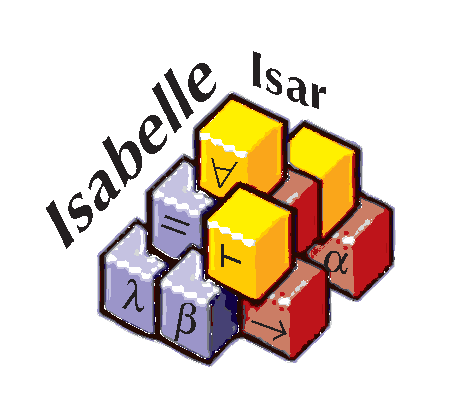
\includegraphics[scale=0.5]{isabelle_isar} \\[4ex] The Isabelle/Isar Reference Manual}
\author{\emph{Markus Wenzel} \\ TU M\"unchen}

\makeindex

\railterm{percent,ppercent,underscore,lbrace,rbrace,llbrace,rrbrace}
\railterm{ident,longident,symident,var,textvar,typefree,typevar,nat,string,verbatim,keyword}

\railalias{ident}{\railtoken{ident}}
\railalias{longident}{\railtoken{longident}}
\railalias{symident}{\railtoken{symident}}
\railalias{var}{\railtoken{var}}
\railalias{textvar}{\railtoken{textvar}}
\railalias{typefree}{\railtoken{typefree}}
\railalias{typevar}{\railtoken{typevar}}
\railalias{nat}{\railtoken{nat}}
\railalias{string}{\railtoken{string}}
\railalias{verbatim}{\railtoken{verbatim}}
\railalias{keyword}{\railtoken{keyword}}

\railalias{name}{\railqtoken{name}}
\railalias{nameref}{\railqtoken{nameref}}
\railalias{text}{\railqtoken{text}}
\railalias{type}{\railqtoken{type}}
\railalias{term}{\railqtoken{term}}
\railalias{prop}{\railqtoken{prop}}
\railalias{atom}{\railqtoken{atom}}

\newcommand{\drv}{\mathrel{\vdash}}
\newcommand{\edrv}{\mathop{\drv}\nolimits}
\newcommand{\Or}{\mathrel{\;|\;}}


\setcounter{secnumdepth}{2} \setcounter{tocdepth}{2}

\pagestyle{headings}
\sloppy
\binperiod     %%%treat . like a binary operator

\renewcommand{\phi}{\varphi}

%\includeonly{generic,refcard}


\begin{document}

\underscoreoff

\maketitle 

\begin{abstract}
  \emph{Intelligible semi-automated reasoning} (\emph{Isar}) is a generic
  approach to readable formal proof documents.  It sets out to bridge the
  semantic gap between any internal notions of proof based on primitive
  inferences and tactics, and an appropriate level of abstraction for
  user-level work.  The Isar formal proof language has been designed to
  satisfy quite contradictory requirements, being both ``declarative'' and
  immediately ``executable'', by virtue of the \emph{Isar/VM} interpreter.
  
  The current version of Isabelle offers Isar as an alternative proof language
  interface layer.  The Isabelle/Isar system provides an interpreter for the
  Isar formal proof language.  The input may consist either of proper document
  constructors, or improper auxiliary commands (for diagnostics, exploration
  etc.).  Proof texts consisting of proper elements only, admit a purely
  static reading, thus being intelligible later without requiring dynamic
  replay that is so typical for traditional proof scripts.  Any of the
  Isabelle/Isar commands may be executed in single-steps, so basically the
  interpreter has a proof text debugger already built-in.
  
  Employing the Isar instantiation of \emph{Proof~General}, a generic Emacs
  interface for interactive proof assistants, we arrive at a reasonable
  environment for \emph{live document editing}.  Thus proof texts may be
  developed incrementally by issuing proof commands, including forward and
  backward tracing of partial documents; intermediate states may be inspected
  by diagnostic commands.
  
  The Isar subsystem is tightly integrated into the Isabelle/Pure meta-logic
  implementation.  Theories, theorems, proof procedures etc.\ may be used
  interchangeably between classic Isabelle proof scripts and Isabelle/Isar
  documents.  Isar is as generic as Isabelle, able to support a wide range of
  object-logics.  Currently, the end-user working environment is most complete
  for Isabelle/HOL.
\end{abstract}

\pagenumbering{roman} \tableofcontents \clearfirst

%FIXME
% - HahnBanach paper
% - Freek Widijk's stuff

%FIXME
\nocite{Rudnicki:1992:MizarOverview}
\nocite{Harrison:1996:MizarHOL}
\nocite{Rudnicki:1992:MizarOverview}
\nocite{Trybulec:1993:MizarFeatures}
\nocite{Syme:1997:DECLARE}
\nocite{Syme:1998:thesis}
\nocite{Syme:1999:TPHOL}
\nocite{Zammit:1999:TPHOL}

\include{intro}
\include{basics}
\include{syntax}
\include{pure}
\include{generic}
\include{hol}

\appendix
\include{refcard}

\begingroup
  \bibliographystyle{plain} \small\raggedright\frenchspacing
  \bibliography{../manual}
\endgroup

\input{isar-ref.ind}

\end{document}


\end{document}


\end{document}


\end{document}
